  \documentclass[12pt,a4paper]{book}
\usepackage[a4paper, top=2.5cm, bottom=2.5cm, left=2.5cm, right=2.5cm, headheight=15pt, headsep=0.5cm]{geometry}
\usepackage{graphicx}
\usepackage{newlfont}
\usepackage{color}
\usepackage{amsmath}
\usepackage{amssymb}
\usepackage{changepage}
\usepackage{fancyhdr}
\usepackage{titlesec}
\usepackage{tikz}
\usepackage{url}      
\usepackage{cancel}   
\usepackage[colorlinks=true, linkcolor=blue, citecolor=green, urlcolor=cyan]{hyperref}     
\usepackage{cleveref}    
\usepackage{bookmark}
\usepackage{multicol}
\usepackage{multirow}
\usepackage{pgfplots}
\usepgfplotslibrary{colormaps}
\usepackage{caption}
\usepackage{subcaption}
\usepackage[justification=centering]{caption}
\usepackage{tensor}
\usepackage{braket}
\usepackage{tabularx}


\newcommand{\Title}{Dissipation of primordial Gravitational Waves and CMB spectral distortions}
\newcommand{\Author}{Luca Morelli}

\newcommand{\defeq}{\stackrel{\text{def}}{=} }
\newcommand{\versor}[1]{\mathbf{\hat{#1}}}

\pgfplotsset{compat=1.18}
\tikzset{>=stealth}
\pagestyle{fancy}
\fancyhead[LE]{\textbf{\nouppercase{\leftmark}}}
\fancyhead[RE]{}
\fancyhead[RO]{\emph{\nouppercase{\rightmark}}}
\fancyhead[LO]{}
\fancyfoot[LE,RO]{\thepage}
\fancypagestyle{plain}{
  \fancyhf{} % clear all header and footer fields
  \fancyfoot[LE,RO]{\thepage} % set page number on left (even) and right (odd)
  \renewcommand{\headrulewidth}{0pt} % optional: remove the header rule line
}
\fancypagestyle{blank}{
  \fancyhf{} % clear all header and footer fields
  \fancyfoot[LE,RO]{\thepage} % set page number on left (even) and right (odd)
  \renewcommand{\headrulewidth}{0pt} % optional: remove the header rule line
}



\cfoot{}
\setlength{\headwidth}{\textwidth}
\usetikzlibrary{arrows.meta, decorations.pathmorphing, positioning, decorations.markings}
% Redefining part display style
\titleformat{\part}[display] 
{\normalfont\Huge\bfseries\centering} 
{\thepart} 
{20pt} 
{\Huge}



\begin{document}
\tikzset{->-/.style={decoration={markings, mark=at position #1 with {\arrow[scale=1.5]{>}}}, postaction={decorate}}}
\frontmatter 
\begin{titlepage}
    \newgeometry{top=1.25cm, bottom=1.25cm, left=2cm, right=2cm}
    \begin{center}
        
\includegraphics[width=65mm]{Logo Unibo.png}
        \vspace{7mm}
        
        {{\bf Department of Physics and Astronomy “A. Righi”\\\vspace{4mm}
        Second cycle degree \\\vspace{7mm}
        \large Physics}}
        \end{center}
        \vspace{23mm}
        \begin{center}
        {\LARGE{\bf \Title}}\\
        \end{center}
        \vspace{50mm} \par \noindent
        \begin{minipage}[t]{0.47\textwidth}
        {\large{\bf Supervisor: \vspace{2mm}\\
        Prof. Roberto Balbinot}\\\\
        \bf Co-Supervisor:
        \vspace{2mm}\\
        Dott. Fabio Finelli\\
        Dott. Matteo Tagliazucchi
        \\}
        \end{minipage}
        %
        \hfill
        %
        \begin{minipage}[t]{0.47\textwidth}\raggedleft 
        {\large{\bf Defended by:
        \vspace{2mm}\\
        \Author   }}
        \end{minipage}
        \vspace{30mm}
        \begin{center}
        \rule[0.5cm]{15.8cm}{0.6mm}
        Graduation Session \\
        Academic Year 2024/2025 
        \end{center}
    \end{titlepage}
\null\thispagestyle{empty}
\newpage
\vspace*{10pt}
\begin{center}
	\large\textbf{Abstract}\normalsize
\end{center}
\vspace*{10pt}
\addcontentsline{toc}{section}{Abstract}
\markboth{Abstract}{Abstract}
\begin{adjustwidth}{1cm}{1cm}

\end{adjustwidth}
\section*{Notations and conventions}
\markboth{}{Notations and conventions}
\addcontentsline{toc}{section}{Notations and conventions}
\vspace*{\fill}
\textbf{Units:} This thesis mainly uses \emph{natural units} $c=\hbar=1$. Only when explicitly stated the the S.I. units are restored.\\  
\textbf{Indexes:} Greek indices $\mu,\nu,\rho,\dots$ denote spacetime components (0--3) of 4-vectors. Latin indices $i,j,k,\dots$ denote purely spatial components (1--3). The \emph{Einstein convention}, for which repeated indexes are summed over, is used. \\
\textbf{Metric:} The signature convention we chose is mostly plus $(-,+,+,+)$. In the Friedmann Robertson Walker metric $a$ is the \emph{scale factor}, $t$ the \emph{cosmic time} and $\tau$ the \emph{conformal time}. We always assume that we live in a \emph{flat universe} ($k=0$).\\
\textbf{Vectors:} the position 4-vector $x^\mu=(x^0,\mathbf x)$ is sometimes represented just by $x$, which should not be confused with the dimensionless frequency. 3-vectors are bold ($\mathbf v$) when the latin index is not written, 3-versos are bold with the upper hat symbol $\versor n$. The dot product $\mathbf{a\cdot b}$ is the euclidean product. \\
\textbf{Total derivatives:} Total derivatives w.r.t cosmic time $t$ are denoted by $\tfrac d{dt}$ or by a dot $\dot f(t)$, while $\tfrac d{d\tau}$ or a prime stands for total derivative w.r.t conformal time. Sometimes the prime is used for derivatives of function of a single variable, in this case the dependence is always indicated $f'(x)$.\\
\textbf{Partial and covariant derivatives:} Partial derivatives are denoted by $\partial_\mu\phi$ or by a comma $\phi_{,\mu}$, while covariant derivatives by the nabla symbol $\nabla_\mu\phi$ or by a semicolon $\phi_{;\mu}$. Bold nabla $\boldsymbol\nabla$ is instead used to denote the 3-dimensional rotor, divergence or Laplacian.
\textbf{Fourier transforms:} Fourier transformed functions are always denoted by a tilde $\tilde f(\mathbf k)$. The measure in momentum space, in our convention, is always divided by a factor $(2\pi)^3$.  \\
\textbf{Power spectra:} we use the convention for which $P_\delta(k)$ is the power spectrum of the generic perturbation $\delta$, while $\mathcal P_\delta(k)=k^3/(2\pi^2) P_\delta(k)$ is the dimensionless power spectrum.  
\tableofcontents

\mainmatter
\setlength{\parskip}{.5em} % Increase paragraph spacing
%\part{The homogeneous universe}
\chapter{The Friedmann Robertson Walker Universe}
Cosmology is based upon two basic symmetry principles:
\begin{itemize}
    \item \textbf{the Copernican Principle}, or that all the observers are on equal footing;
    \item \textbf{the Cosmological Principle}, which states that the universe, at the largest scales, is homogeneous and isotropic.
\end{itemize}
These principles may not seem consistent with physical reality: clearly the core of a star is very different from empty space or even from the interior of planets, but in order to describe the dynamics of the whole universe we need to make some simplifying assumptions. Observations, for example of the distribution of galaxies or of the cosmic microwave background radiation, show that at large scales, on average, the universe looks the same in all directions. The Copernican Principle then implies that all observers should see an isotropic universe, thus we can claim that all points of the universe should also look the same. Again we should stress that these are just assumptions that, at some large scale, we think can become adequate to approximate the description of space, allowing us to reduce significantly the degrees of freedom that we have to study.
\section{The geometry of the universe}
We now have to translate the proprieties of isotropy and homogeneity to the language of General Relativity, namely differential geometry and manifolds.\\ Notice that the two above principles refer only to the universe, or better, to space at a fixed time, therefore it is space which is really isotropic and homogeneous, while time has no particular symmetries.\\
Hence, we will assume that space is \textbf{maximally symmetric}, which means that it possesses the maximum number of independent Killing vectors. In fact, homogeneity guarantees 3 Killing vectors, associated to the 3 possible space translations, while isotropy guarantees other 3 Killing vectors, associated to the 3 rotations around a point, and the maximum number of independent Killing vectors for a 3D manifold is indeed 6 (this is proven in Appendix \ref{app:MaxSymm}).
In the next sections we will study first how to describe a spacetime with the above proprieties, then we will work out the dynamics that the Einstein field equations give to it.
\subsection{The Friedmann Robertson Walker metric}
We will now proceed constructing charts (coordinates) that are the more convenient to describe the assumed geometry. The main goal of this section is to find the most general form of the metric of an isotropic and homogeneous universe.

To start, consider a space-like hypersurface $\Sigma$ (a volume in this case), which is a slice of the spacetime manifold, corresponding to space (the universe) at a fixed time. On this hypersurface we choose one chart with coordinates $x^\mu=(0,x^1,x^2,x^3)$.\\ For each point $P\in\Sigma$ we pick a vector $\vec n$ that is orthogonal to $\Sigma$ (it should be orthogonal to each vector of the tangent space, in $P$, of the submanifold defined by $\Sigma$) such that those are normalized to $-1$ (since they are orthogonal to a space-like hypersurface).\\ In each point $P$ the following Cauchy problem defines a unique geodesic for which $\vec n$ is the tangent vector,
\begin{equation}\label{Chaucy problem}
    \begin{cases}
        \big(\nabla_{\vec n}\vec n\big)^\mu=\frac{d^2x^\mu}{dt^2}+\Gamma_{\nu\lambda}^{\mu}\frac{dx^\nu}{dt}\frac{dx^\lambda}{dt}=0,\\\frac{dx^\mu}{dt}\big|_{P}=n^\mu\big|_P,\\x^\mu(0)=x^\mu\big|_P.
    \end{cases}
\end{equation}
We can extend our initial chart, in a neighborhood of $\Sigma$, assigning to each point $Q$ the coordinates $x^\mu=(t,x^1,x^2,x^3)$, where $t$ is the value in $Q$ of the geodesic parameter and $(0,x^1,x^2,x^3)$ are the coordinates of the point $P$, from which the geodesic starts. These coordinates will eventually fail once some geodesics, from our construction, will meet and intersect.

We now want to describe the metric of our spacetime manifold using one of these charts. To do so we will take the chart induced basis of each tangent space $(\partial_t,\partial_1,\partial_2,\partial_3)$ and then label them:
\begin{equation*}
    \partial_t=\vec n,\qquad \partial_i= \vec Y_{(i)},
\end{equation*}
where $\partial_t$ is by construction the normal vector field we have defined, since $\vec n$ is tangent to each geodesic by \eqref{Chaucy problem} and then is parallel transported along them.\\
Using this basis, the first component of the metric reads, by our initial construction and because scalar products of parallel transported vectors is preserved by metric connection,
\begin{equation*}
    g_{tt}=g(\partial_t,\partial_t)=n^\mu n_\mu=-1.\label{gen gtt}
\end{equation*} 
On $\Sigma$, from our construction hypothesis $\vec{n}\perp\Sigma $, the time-spacial mixed components read 
\begin{equation*}
    g_{ti}=g(\partial_t,\partial_i)=n_\mu Y^\mu_{(i)}=0.\label{gen gti}
\end{equation*} 
We can prove that this holds also outside $\Sigma$ by evaluating its covariant derivative along one of the geodesics we constructed
\begin{align*}
    n^\nu\nabla_\nu\Big(n_\mu Y_{(i)}^\mu\Big)&=n^\nu n_\mu \nabla_\nu Y_{(i)}^\mu+\cancel{Y_{(i)}^\mu n^\nu  \nabla_\nu n_\mu}\\
    &=Y^\nu_{(i)}n_\mu\nabla_\nu n^\mu\\
    &=\frac{1}{2}\Big(Y^\nu_{(i)}n_\mu\nabla_\nu n^\mu+Y^\nu_{(i)}n_\mu\nabla_\nu\big(g^{\mu\lambda}n_{\lambda}\big)\Big)\\
    &=\frac{1}{2}\Big(Y^\nu_{(i)}n_\mu\nabla_\nu n^\mu+\cancel{Y^\nu_{(i)}n_\mu\nabla_\nu\big(g^{\mu\lambda}\big)n_{\lambda}}+Y^\nu_{(i)}n_\mu g^{\mu\lambda}\nabla_\nu n_{\lambda}\Big)\\
    &=\frac{1}{2}\big(Y^\nu_{(i)}n_\mu\nabla_\nu n^\mu+Y^\nu_{(i)}n^\lambda\nabla_\nu n_{\lambda}\big)\\
    &=\frac{1}{2}Y^\nu_{(i)}\nabla_\nu\big(n^\lambda n_\lambda\big)=0,
\end{align*}
in which we used (in order): the geodesic equation $n^\nu  \nabla_\nu(n_\mu )=0$, that coordinates vectors commute, so that $[\vec n,\vec Y_{(i)}]^\mu=n^\nu \nabla_\nu( Y_{(i)}^\mu)-Y^\nu_{(i)}\nabla_\nu(n^\mu)=0$\footnote{The Christoffel symbols cancel out, due to symmetric connection, leaving only partial derivatives.}, the metric connection condition $\nabla g=0$, and last that, being $n^\mu n_\mu=-1$, its derivative vanishes.\\
Summing up the above results, we can write the metric as
\begin{equation*}
    ds^2=-dt^2+g_{ij}dx^i dx^j.
\end{equation*}
In this expression the absence of the mixed terms $dt\ dx^i$ reflects that there exist a family of hypersurfaces, defined by $t=$ const, that are all orthogonal to the vector field $\vec n$. These represent the evolved universe at different times.\\
At this stage, the spatial components of the metric can depend on all the coordinates of the chart we have introduced. If we consider how time evolution could affect the spatial terms we can deduce that all the components $g_{ij}$ should scale in the same way, a different scaling would have been against the assumption of isotropy. We will write explicitly the time dependence as
\begin{equation*}
    ds^2=-dt^2+a^2(t)g_{ij}dx^i dx^j.
\end{equation*} 
Let's now take into account that each space hypersurface is a maximally symmetric submanifold. 
As showed in Appendix \ref{app:MaxSymm}, maximally symmetric manifolds have the peculiar propriety that, due to their high number of symmetries, the Riemann tensor reduces (in 3 dimensions) to 
\begin{equation*}
    ^{(3)}R_{ijkl}=\frac{^{(3)}R}{6}(g_{ik}g_{jl}-g_{il}g_{jk}),
\end{equation*}
in which the $^{(3)}$ is used to signal that these are tensors referred to the submanifold $\Sigma$ and $^{(3)}R$ is their Ricci scalar. The Ricci tensor thus reads:
\begin{equation}\label{maxsymRicci}
    ^{(3)}R_{ij}=\frac{^{(3)}R}{6}(3g_{ij}-g^{lk}g_{il}g_{jk})=\frac{^{(3)}R}{3}g_{ij}.
\end{equation}
With this relation we can further to determine the metric without using the Einstein field equations yet.
To simplify the metric, we can note that, being maximally symmetric, each space submanifold will also have spherical symmetry. This allows us to write the metric in spherical coordinates as
\begin{equation*}
    ds^2=-dt^2+a(t)^2\big[e^{2\beta(r)}dr^2+e^{2\gamma(r)}r^2(d\theta^2+\sin^2\theta\ d\phi^2)\big],
\end{equation*}  
where $\beta(r),\ \gamma(r)$ are some unknown functions that depend only on the radial coordinate due to spherical symmetry. Note that we exploited the exponential in order to preserve the signature. Lastly, the angular part, $d\Omega^2= d\theta^2+\sin\theta\ d\phi^2$, must scales with an overall factor $e^{2\gamma}$, in order to maintain sphere to be perfectly round.\\
We can simplify this metric even more by scaling the radial coordinate
\begin{equation*}
    r\rightarrow e^{-\gamma(r)}r,\qquad dr\rightarrow \bigg(1-r\frac{d\gamma}{dr}\bigg)e^{-\gamma(r)}dr,
\end{equation*}
in this way the metric becomes
\begin{equation*}
    ds^2=-dt^2+a^2(t)\bigg[\bigg(1-r\frac{d\gamma}{dr}\bigg)^{2}e^{2(\beta(r)-\gamma(r))}dr^2+r^2(d\theta^2+\sin^2\theta\ d\phi^2)\bigg].
\end{equation*}
Since $g_{rr}$ must always be non-negative, we can define a function $\alpha(r)$, such that $e^{2\alpha}=\big(1-r\frac{d\gamma}{dr}\big)^{2}e^{2(\beta(r)-\gamma(r))}$, so that the metric reads
\begin{equation*}
    ds^2=-dt^2+a^2(t)\big[e^{2\alpha(r)}dr^2+r^2(d\theta^2+\sin^2\theta\ d\phi^2)\big].
\end{equation*}
Now, we can evaluate the Christoffel symbols of the metric restricted to the universe submanifold (because with this construction the time component has no dynamics):
\begin{align}\label{eq:RWL3Christoffel}
    ^{(3)}\Gamma_{rr}^r&=\frac{d\alpha}{dr},\qquad^{(3)}\Gamma_{r\theta}^\theta=\frac{1}{r},\qquad^{(3)}\Gamma_{\theta\theta}^r=-re^{-2\alpha},\qquad^{(3)}\Gamma_{rr}^r=\frac{\cos\theta}{\sin\theta},\nonumber\\
    ^{(3)}\Gamma_{r\phi}^\phi&=\frac{1}{r},\qquad^{(3)}\Gamma_{\phi\phi}^r=-re^{-2\alpha}\sin^2\theta,\qquad^{(3)}\Gamma_{\phi\phi}^\theta=-\sin\theta\cos\theta,
\end{align}
all the others are zero or deducible from the symmetries of the above.\\ We then obtain the non-vanishing components of the Riemann tensor are:
\begin{align}\label{eq:RWL3Riemann}
    ^{(3)}R^r_{\theta r\theta}&=re^{-2\alpha}\frac{d\alpha}{dr},\nonumber\\
    ^{(3)}R^r_{\phi r\phi}&=re^{-2\alpha}\sin^2\theta\frac{d\alpha}{dr},\nonumber\\
    ^{(3)}R^\theta_{\phi \theta\phi}&=(1-e^{-2\alpha})\sin^2\theta.
\end{align}
Lastly, we can get the Ricci tensor:
\begin{equation}\label{eq:RWL3Ricci}
    ^{(3)}R_{rr}=\frac{2}{r}\frac{d\alpha}{dr},\qquad ^{(3)}R_{\theta\theta}=e^{-2\alpha}\bigg[r\frac{d\alpha}{dr}-1\bigg]+1,\qquad ^{(3)}R_{\phi\phi}=\sin^2\theta R_{\theta\theta}.
\end{equation}
Combining the expression for the Ricci tensor \eqref{maxsymRicci} and the one above \eqref{eq:RWL3Ricci}, we end up with two differential equations that can be solved to determine the metric
\begin{align*}
    ^{(3)}R_{rr}&=\frac{^{(3)}R}{3}g_{tt}\quad\Rightarrow\quad\boxed{\frac{2}{r}\frac{d\alpha}{dr}=\frac{^{(3)}R}{3}e^{2\alpha}}\\ ^{(3)}R_{ij}&=\frac{^{(3)}R}{3}g_{ij}\quad\Rightarrow\quad \boxed{e^{-2\alpha}\bigg[r\frac{d\alpha}{dr}-1\bigg]+1=\frac{^{(3)}R}{3}r^2}.
\end{align*}
Since we have two equations for one unknown, substituting the first equation into the second one, we can obtain an initial condition for the former
\begin{equation*}
    \frac{d\alpha}{dr}=\frac{^{(3)}R}{6}re^{2\alpha},\qquad\qquad e^{-2\alpha}\bigg[\frac{^{(3)}R}{6}r^2e^{2\alpha}-1\bigg]+1=\frac{^{(3)}R}{3}r^2.
\end{equation*}
To solve this differential equation we start by defining $k\defeq^{(3)}R/6$, and then we integrate
\begin{align*}
    \int e^{-2\alpha}\ d\alpha=\int kr\ dr\quad \Rightarrow\quad e^{-2\alpha}=-kr^2+C,
\end{align*}
then, to determine $C$ we plug this solution into the initial condition
\begin{align*}
    2kr^2&=e^{-2\alpha}\bigg[kr^2e^{2\alpha}-1\bigg]+1=kr^2-e^{-2\alpha}+1\\
       &=kr^2+kr^2-C+1=2kr^2-C+1,\quad \Rightarrow\quad \boxed{C=1}.
\end{align*}    
In this way we have obtained the \textbf{Friedmann Robertson Walker metric} (FRW metric)
\begin{equation}\label{eq:RWMetric}
    ds^2=-dt^2+a^2(t)\bigg[\frac{dr^2}{1-kr^2}+r^2(d\theta^2+\sin^2\theta\ d\phi^2)\bigg],
\end{equation}
notice that to obtain this metric we never used the Einstein field equation but only geometrical proprieties of spacetime, deduced from the cosmological principle, therefore this metric is totally generic once we assume such principle.\\
The coordinates $(t,r,\theta,\phi)$ are called \textbf{comoving coordinates}, since these precise choice makes manifest the isotropy and homogeneity of the universe, that wouldn't be manifest in a moving reference frame with respect to the universe content.
Two parameters appear in this metric:
$a(t)$, the \textbf{cosmic scale factor}, which measure how distances, since it multiplies the spatial part of the metric, change with time, and
$k$, the \textbf{curvature constant}, that is proportional to the Ricci scalar of each universe submanifold and thus measures the curvature of space.\\
These parameters can be rescaled as follows, without affecting the metric \eqref{eq:RWMetric},
\begin{equation*}
    r\rightarrow\lambda r,\qquad a\rightarrow\lambda^{-1} a,\qquad k\rightarrow\lambda^{-2} k,
\end{equation*}
this allows to give dimensions of a length arbitrarily to $r$ or to $a$.

We will now give some interpretation to the curvature constant that appears in the Friedmann Robertson Walker metric \eqref{eq:RWMetric}. First, it is useful to use the scale invariance of the metric to reduce the possible values of this parameter so that it is just its sign to determine the curvature. Rescaling as follows 
\begin{equation*}
    r\rightarrow\sqrt{|k|}r,\qquad a\rightarrow\frac{a}{\sqrt{|k|}},\qquad k\rightarrow\frac{k}{|k|},
\end{equation*}  
$k$ can now only assume the following values $\{-1,0,+1\}$. \\
Let's now discuss the geometry associated to each value of $k$, we will focus just on the spatial metric $d\sigma^2=\frac{dr^2}{1-kr^2}+r^2(d\theta^2+\sin^2\theta\ d\phi^2)$.
\begin{itemize}
    \item \textbf{Flat universe}, for $k=0$, the metric reduces to usual metric of $\mathbb{R}^3$ in spherical coordinates $$d\sigma^2= dr^2+r^2(d\theta^2+\sin^2\theta\ d\phi^2)$$ which correspond to a flat universe.
    \item \textbf{Closed universe}, for $k=+1$, the metric can be reduced to a more familiar one introducing $$d\chi=\frac{dr}{\sqrt{1-r^2}}\quad\Rightarrow\quad r=\sin\chi,$$$$d\sigma^2=d\chi^2+\sin^2\chi(d\theta^2+\sin^2\theta\ d\phi^2),$$which makes manifest that the radial coordinate is bounded\footnote{This behavior is signaled by the fact that in the previous chart the metric was singular for $r=1$.} ($r\in[0,+1]$) and the metric is the one of a $3$-dimensional sphere.
    \item \textbf{Open universe}, for $k=-1$, the metric can be better understood by introducing$$d\chi=\frac{dr}{\sqrt{1+r^2}}\quad\Rightarrow\quad r=\sinh\chi,$$$$d\sigma^2=d\chi^2+\sinh^2\chi(d\theta^2+\sin^2\theta\ d\phi^2),$$ which shows that $r$ is not bounded, and the metric takes the form of the one of a $3$-dimensional hyperboloid.
\end{itemize}
The value of $k$ will be determined by the energy content of the universe, through the Einstein field equations.

Since in the following sections we will need the metric connection and the Ricci tensor, we are going just to calculate them now.\\
The Christoffel symbols of the Robertson Walker metric \eqref{eq:RWMetric} are
\begin{align}
    &\Gamma^0_{11}=\frac{a\dot{a}}{1-kr^2}, \quad&\Gamma^1_{11}=\frac{kr}{1-kr^2},\nonumber\\&\Gamma^0_{22}=a\dot{a}r^2, \quad&\Gamma^0_{33}=a\dot{a}r^2\sin^2\theta,\nonumber\\&\Gamma^1_{01}=\Gamma^2_{02}=\Gamma^3_{03}=\frac{\dot{a}}{a}, \quad &\Gamma^1_{22}=-r(1-kr^2),\nonumber\\&\Gamma^1_{33}=-r(1-kr^2)\sin^2\theta, \quad &\Gamma^2_{12}=\Gamma^3_{13}=\frac{1}{r},\nonumber\\&\Gamma^2_{33}=-\sin\theta\cos\theta, \quad &\Gamma^2_{23}=\cot\theta,\label{eq:RWChristoffel}
\end{align}
the ones that are not listed are zero or obtainable from the symmetry of the connection.\\
From the above Christoffel symbols, the non-zero components of the Ricci tensor are
\begin{align}
    R_{00}&=-3\frac{\ddot a}{a},\nonumber\\
    R_{11}&=\frac{a\ddot{a}-2\dot a+2k}{1-kr^2},\nonumber\\
    R_{22}&=r^2(a\ddot{a}-2\dot a+2k),\nonumber\\
    R_{33}&=r^2(a\ddot{a}-2\dot a+2k)\sin^2\theta.\label{eq:RWRicci}
\end{align}
\subsection{Dynamical effects in the Robertson Walker universe}
With the Robertson Walker metric \eqref{eq:RWMetric} in our hand it is time to study the consequences of having allowed spacetime to have a dynamics. In this section we will work with an arbitrary cosmic factor, however we will also use as reference our universe in which we observe an expansion described by an increasing $a(t)$. Keep in mind that, from now on, we will use the convention that at $t=t_\text{today}$ the cosmic scale factor is unitary.
\subsubsection{Hubble Law}
Let's start by evaluating the distance between two points: FRW metric gives 
$$d(t)=a(t)\int_{r_1}^{r_2}\frac{dr}{\sqrt{1-kr^2}}.$$
Notice that the above implies that distances can now change overtime: in the case of our universe they increase resulting in the expansion of the universe. This suggests that the comoving coordinates are not really physical, since they represent fixed points that appear to be moving. We thus define the \textbf{physical coordinates} by multiplying the comoving ones by the cosmic scale factor, this allows to describe a non-zero physical velocity for an object at fixed comoving coordinates
$$\mathbf{x}_\text{phy}\defeq a(t)\mathbf{x} \quad\Rightarrow\quad \mathbf{v}_\text{phy}\defeq\dot{\mathbf{x}}_\text{phy}=\frac{\dot a}{a} \mathbf{x}+a(t)\mathbf{v}.$$
This is exactly what Hubble in 1929 \cite{1929PNAS...15..168H} observed by studying the motion of far galaxies: a linear relation between observed velocities and the distance between us and these galaxies. The factor of proportionality is nowadays measured to be $(\dot a/a)(t_0)=H_0\approx70$ km s$^{-1}$ Mpc$^{-1}$ and it is called \textbf{Hubble parameter}, this tells us that for each Megaparsec of distance an object appears to be moving with a physical velocity of $70$ km/s, due to the expansion of the universe. Indeed, by assuming a negligible peculiar velocity of the observed galaxy (typically hundreds of km/s) the physical velocity reads
\begin{equation}
    \label{eq:Hubble_Law}
    \mathbf{v}_\text{phy}=H_0\mathbf{x}
\end{equation}
which is called the \textbf{Hubble law}. Note that there is no obstacle for the physical velocity of a far enough object to exceed the speed of light: however this does not contradict special relativity since this is an effect that arises in our reference frame which is only locally inertial. For two objects at the same arbitrary distance from us, their relative velocity will always be less than the speed of light.
\subsubsection{Cosmological redshift}
All our observations, from astronomical objects, come in the form of light or, more recently, gravitational waves. This means that the notion of physical distances and velocities could not be enough to describe all the effects that could affect our observations. Knowing how the motion on \emph{null geodesics} occurs is also needed. The FRW metric gives $$dt=\pm a(t)\frac{dr}{\sqrt{1-kr^2}}$$ that allows for the comoving distance between two objects to be related to the time needed by light to travel from one to the other. Now, suppose that a far object emits a periodic pulse of light each $\delta t_{\text{em}}$ seconds and let's allow for an arbitrary time between consecutive observations $\delta t_{\text{obs}}$ on the Earth. The above relation allows us to find the latter from the former.
\begin{figure}
    \centering
    \begin{tikzpicture}[>=Stealth]
  % Axes
  \draw[->,thick] (0,0) -- (4,0) node[below right] {$r$};
  \draw[->,thick] (0,-0.5) -- (0,4) node[left] {$t$};

  % Grey dashed vertical line on the right
  \draw[gray, thick, dashed] (3,0) node[below, black] {$r_1$} -- (3,4);

  \foreach \i in {0,...,3} {
        \draw[yellow, ultra thick] (0,1+\i*0.85) -- (3,0.5+\i*0.7);
  }
  \draw[yellow, ultra thick] (1,4) -- (3,0.5+4*0.7);

  % 5 points on the left vertical axis
  \foreach \i in {0,...,3} {
    \fill (0,1+\i*0.85) circle (2pt);
  }

  \foreach \i in {0,...,4} {
    \fill (3,0.5+\i*0.7) circle (2pt);
  }

  
  % Labels for the points
  \node[right] at (0,1) {$t_1$};
  \node[left] at (3,0.5) {$t_0$};
  \foreach \i in {0,...,2} {
    % Double arrows for delta t_obs
    \draw[<->] (-0.25,1+\i*0.85) -- (-0.25,\i*0.85+1.85);
    \node[left] at (-0.3,1.425+\i*0.85) {$\delta t_\text{obs}$};
  }
  \foreach \i in {0,...,3} {
    % Double arrows for delta t_em
    \draw[<->] (3.25,.5+\i*0.7) -- (3.25,\i*0.7+1.2);
    \node[right] at (3.3,0.85+\i*0.7) {$\delta t_\text{em}$};
  }
\end{tikzpicture}
\caption{Graphical depiction of the emission and observation of light pulses in FRW spacetime. Time intervals are not in scale.\label{fig:redshift}}
\end{figure}
Indeed, if at some time $t_0$ a first signal is emitted and then received by us at some time $t_1$, so that\footnote{We used the $-$ sign since the motion occurs from the galaxy to us at the center of the reference frame.}
$$\int_{t_1}^{t_0}\frac{dt}{a(t)}=\int_{0}^{r_1}\frac{dr}{\sqrt{1-kr^2}},$$ then a second pulse of light would be emitted at $t_0+\delta t_{\text{em}}$ and received at $t_1+\delta t_{\text{obs}}$ (Fig. \ref{fig:redshift}), hence giving $$\int_{t_1+\delta t_{\text{obs}}}^{t_0+\delta t_{\text{em}}}\frac{dt}{a(t)}=\int_{0}^{r_1}\frac{dr}{\sqrt{1-kr^2}}.$$
Note that in both the above expressions the right-hand side is time independent and determined only by the comoving coordinates of the emitting and receiving objects. Equating the above and by splitting the second integral, we get
\begin{align*}
    \int^{t_1}_{t_0}\frac{dt}{a(t)}=\int^{t_1+\delta t_{\text{em}}}_{t_0+\delta t_{\text{obs}}}\frac{dt}{a(t)}=\int_{t_0+\delta t_{\text{em}}}^{t_0}\frac{dt}{a(t)}+\int^{t_1}_{t_0}\frac{dt}{a(t)}+\int^{t_1+\delta t_{\text{obs}}}_{t_1}\frac{dt}{a(t)}
\end{align*}
that, by assuming $\delta t_{\text{em}}$ and $\delta t_{\text{obs}}$ to be small (so that the remaining integral can be approximated by the integrand times $\delta t$) we find:
\begin{equation}
    \label{eq:delta_t1/delta_t2}
    \frac{\delta t_{\text{em}}}{\delta t_{\text{obs}}}=\frac{a(t_{\text{em}})}{a(t_{\text{obs}})}.
\end{equation}
This means that, as the universe expands, $a(t)$ increases and the elapsed time between consecutive observations becomes greater than the time between emissions.

This may seem a less important effect, however, when considering the wave nature of light, what we call \textbf{redshift} arises and becomes an essential tool for our observations. Consider $\delta t$ as the period related to a specific wave of light (or a gravitational wave since both move on null geodesics), this time is proportional to its wavelength ($\lambda= c\delta t$): ultimately this means that the effect described above results in a difference between the emitted wavelength and the observed one.\\Redshift of far objects is measured by the \textbf{redshift parameter} as
\begin{equation}
    \label{eq:redshift}
    z\defeq\frac{\lambda_{\text{obs}}-\lambda_{\text{em}}}{\lambda_{\text{em}}}=\frac{1-a(t_{\text{em}})}{a(t_\text{em})}\quad\Rightarrow\quad 1+z=\frac{1}{a(t_{\text{em}})},
\end{equation}
where we used that $\lambda(t)\propto a(t)$ and the convention $a(t_\text{obs})=1$. This shows that as the universe expands the light that comes from far objects is shifted, in its spectrum, towards red wavelengths. Further they are, more time for light is needed to reach us and $t_\text{em}$ gets pushed away from today increasing the observed redshift. This connection allows us referring to time in terms of redshifts: today corresponds to $z=0$, $z=1$ corresponds to when the universe was half its current size and as $z$ increases we go back in time.

Lastly, let us mention how redshift is measured. This is accomplished by studying the spectrum of observed galaxies: for each object we can predict its absorption lines (by knowing its chemical composition) that for far objects appear all \emph{"redshifted"} in the same way. By comparison with the spectrum of the same gasses on the Earth we obtain $z$. 
\section{The Friedmann equations}
We now want to determine the dynamics of the parameters appearing in the Robertson Walker \eqref{eq:RWMetric} metric knowing the energy content of the universe. The connection between the metric and the energy is given by the \emph{Einstein field equations}
\begin{equation}\label{eq:EFE}
    R_{\mu\nu}-\frac{1}{2}Rg_{\mu\nu}=8\pi GT_{\mu\nu},
\end{equation}
where it appears the energy-momentum tensor $T^{\mu\nu}$.
\subsection{Cosmic fluids}
The simplest model for the content of the universe is a \emph{perfect fluid} of energy and matter. A perfect fluid, in general, is described by an energy-momentum tensor given by
\begin{equation}\label{eq:PerfectFluidEMTensor}
    T^{\mu\nu}=(\rho+p)U^\mu U^\nu+pg^{\mu\nu},
\end{equation}
where $\rho$ is the energy density of the fluid, $p$ the pressure and $U^\mu$ the $4$-velocity of a particle of the fluid.\\When we described the coordinates appearing in the Robertson Walker metric, we anticipated that those were comoving coordinates with respect to the content of the universe (so that in that reference frame the metric would be manifestly isotropic and homogeneous). In the reference frame associated to those coordinates, the fluid is at rest, thus its energy-momentum tensor takes the form
\begin{equation}
    U^\mu=(1,0,0,0),\quad\Rightarrow\quad
    T_{\mu\nu}=\begin{pmatrix}
        \rho&0&0&0\\
        0&&&\\
        0&&g_{ij}p&\\
        0&&&
    \end{pmatrix},
    \quad T^\mu\phantom{} _\nu=\text{diag}(-\rho,p,p,p)\label{eq:EMTensorCosmicFluid}
\end{equation}
Even before plugging everything in the Einstein equations, we can study the energy conservation of this fluid, which reads
\begin{align}\label{eq:ConservationEnergy}
    0&=\nabla_\mu T^\mu\phantom{} _0\nonumber\\&=\partial_\mu T^\mu\phantom{} _0+\Gamma^\mu_{\mu\lambda}T^\lambda\phantom{} _0-\Gamma^\lambda_{\mu0}T^\mu\phantom{} _\lambda\nonumber\\
    &=\partial_0 T^0\phantom{} _0+\Gamma^\mu_{\mu0}T^0\phantom{} _0-\Gamma^\lambda_{\mu0}T^\mu\phantom{} _\lambda\nonumber\\
    &=-\dot\rho-3\frac{\dot a}{a}\rho-3\frac{\dot a}{a}p\nonumber\\
    &=-\dot\rho-3\frac{\dot a}{a}(\rho+p),
\end{align}
in which we used that $T^\mu\phantom{}_\nu$ is diagonal, and the Christoffel symbols \eqref{eq:RWChristoffel}.

From now, we assume that the fluid follows some simple equation of state, as
\begin{equation}\label{eq:EquationState}
    p=\omega\rho,\qquad\omega=\text{constant}.
\end{equation}
Inserting this into the conservation of energy equation \eqref{eq:ConservationEnergy} we find
\begin{equation*}
    \frac{\dot\rho}{\rho}=-3(1+\omega)\frac{\dot a }{a},
\end{equation*}
that can be solved to obtain how the energy density of the fluid scales as the universe expands:
\begin{align*}
    \int \frac{d\rho}{\rho}=-3(1+\omega)\int \frac{da}{a} \quad\Rightarrow\quad \boxed{\rho=\rho_0a^{-3(1+\omega)}}.
\end{align*}

To better grasp the physics of our construction let's study the evolution of some simple cases of fluids.
\begin{itemize}
    \item \textbf{Dust}: this kind of fluid is defined as a set of collisionless, non-relativistic particles, that therefore will have zero pressure:$$p_d=\omega_d\rho_d=0,\quad\Rightarrow\quad \omega_d=0\quad\Rightarrow\quad\rho_d=\frac{E}{V}=\rho_{0}a^{-3}.$$ We can appreciate how, for dust, the energy density scales with the volume ($V \propto  a^3$), keeping constant the total energy. This sort of fluid can be used to model groups of stars and galaxies, for which the pressure is negligible, compared to the energy density.
    \item \textbf{Radiation}: in this case we want to describe massless particles or ultra-relativistic ones, which can be approximated to be massless. We can obtain an equation of state for this fluid by first observing that the $T^{\mu\nu}$ is traceless for E-M fields $$T^\mu\phantom{}_\mu=F^{\mu\lambda}F_{\mu\lambda}-\frac{1}{4}g^\mu\phantom{}_\mu F^{\lambda\sigma}F_{\lambda\sigma}=0,$$ at the same time the \eqref{eq:EMTensorCosmicFluid} gives that $$T^\mu\phantom{}_\mu=-\rho+3P,\quad\Rightarrow\quad P_r=\frac{1}{3}\rho_r,$$ which implies $\omega_r=\frac{1}{3}$. Therefore, the energy density of radiation scales as$$\rho_r=\rho_0a^{-4},$$ that means that for radiation the total energy is not conserved. We interpret this as the fact that, while the universe expands, radiation gets redshifted.
    \item \textbf{Vacuum or dark energy}: this last type of cosmic fluid is quite a strange one, the equation of state for this fluid is $$p_v=-\rho_v,\quad \Rightarrow\quad \omega_v=-1.$$ This means that the energy density, as well as the pressure, as the universe expands, remains constant. Sometimes this is not considered a content of the universe, and it is referred as the \emph{cosmological constant} $\Lambda$: $$\rho_v=\frac{\Lambda}{8\pi G}.$$
\end{itemize}
Initially, it was thought that the universe could be described just but dust and radiation: a radiation dominated universe that then transitioned into a matter dominated. This was supported by the fact that $\rho_r\propto a^{-4}$ decrease faster than $\rho_d\propto a^{-3}$, as the universe expands.\\ Nowadays, we know that the expansion of the universe is accelerating, and this led to the introduction of the dark energy, to account for this behavior.
\subsection{Firedmann equations}
Now that we characterized the main types of fluids that we can use to model the content of the universe, we can proceed to derive the equations governing the time evolution of the universe.

First we want to simplify a bit Einstein equations \eqref{eq:EFE}: from the trace of both sides of the equation we get
\begin{equation*}
    R-\frac{4}{2}R=8\pi GT\quad\Rightarrow\quad R=-8\pi GT,
\end{equation*}
where $T=T^\mu\phantom{}_\mu$, plugging this result in the field equations \eqref{eq:EFE}, we can remove the Ricci scalar:\begin{equation*}
    R_{\mu\nu}=8\pi G\bigg(T_{\mu\nu}-\frac{1}{2}Tg_{\mu\nu}\bigg).
\end{equation*}
From the Ricci tensor components of the Robertson Walker metric \eqref{eq:RWRicci} and the energy momentum tensor \eqref{eq:EMTensorCosmicFluid} we can obtain two equations:
\begin{itemize}
    \item the $\mu\nu=00$ component leads to
    \begin{align*}
        -3\frac{\ddot a}{a}&=8\pi G\bigg[-\rho-\frac{1}{2}(-\rho+3p)\bigg]\\&=4\pi G(\rho+3p);
    \end{align*}
    \item the $\mu\nu=ij$ components lead to
    \begin{align*}
        \frac{a\ddot a+2\dot a^2+2k}{a^2}g_{ij}&=8\pi G\bigg[pg_{ij}-\frac{1}{2}g_{ij}(-\rho+3p)\bigg]\\&=4\pi G(\rho-p)g_{ij}.
    \end{align*}
\end{itemize}
Substituting the former into the latter we find
\begin{align}
   -\frac{4}{3}\pi G(\rho+3p) +\frac{2\dot a^2+2k}{a^2}&=4\pi G(\rho-p)\nonumber\\\frac{2\dot a^2+2k}{a^2}&=4\pi G\frac{4}{3}\rho\nonumber
\end{align}
\begin{equation}
    \boxed{\bigg(\frac{\dot a }{a}\bigg)^2=\frac{8\pi G}{3}\rho-\frac{k}{a^2}}\label{eq:Friedmann1},
\end{equation}
which is the \textbf{first Friedmann equation}, while from the $00$ component alone we get the \textbf{second Friedmann equation}
\begin{equation}
    \label{eq:Friedmann2}\boxed{\frac{\ddot a}{a}=-\frac{4\pi G}{3}(\rho+3p)}.
\end{equation}
The first, which is the one that is usually referred as the Friedmann equation, will determine the time evolution of the scale factor $a(t)$. To solve it, it is enough to know the dependence $\rho(a)$, that we previously discussed.
\subsection{Universe geometry and its density}
Usually, the first Friedmann equation \eqref{eq:Friedmann1} is expressed in terms of some cosmological parameters:
\begin{itemize}
    \item the \textbf{Hubble parameter}, $H=\frac{\dot a}{a}$, which measure the rate of expansion,
    \item the \textbf{critical density}, $\rho_{\text{crit}}=\frac{3H^2}{8\pi G}$
    \item the \textbf{density parameter}, $\Omega=\frac{8\pi G}{3H^2}\rho=\frac{\rho}{\rho_{\text{crit}}}$.
\end{itemize}
In this way \eqref{eq:Friedmann1} explicitly relates the matter content of the universe with its geometry (flat. open or closed). Indeed, inserting the above parameters in \eqref{eq:Friedmann1} it reads
\begin{equation}
    \boxed{\Omega-1=\frac{k}{H^2a^2}},
\end{equation}
from which we can distinguish 3 distinct cases:
\begin{itemize}
    \item $\rho<\rho_{\text{crit}}\quad\Leftrightarrow\quad \Omega<1 \quad\Leftrightarrow\quad k<0 \quad\Leftrightarrow\quad $\emph{open universe},
    \item  $\rho=\rho_{\text{crit}}\quad\Leftrightarrow\quad \Omega=1 \quad\Leftrightarrow\quad k=0 \quad\Leftrightarrow\quad $\emph{flat universe},
    \item  $\rho>\rho_{\text{crit}}\quad\Leftrightarrow\quad \Omega>1 \quad\Leftrightarrow\quad k>0 \quad\Leftrightarrow\quad $\emph{closed universe}.
\end{itemize} 
Observations suggest that now, for our universe, $k\approx0$. Therefore, we will always consider flat geometry. In this case the dynamics of the universe is determined by $$\bigg(\frac{\dot a }{a}\bigg)^2=\frac{8\pi G}{3}\rho. $$\pagebreak
Depending on the different cosmic fluids the universe evolves mainly in three different ways.
\begin{itemize}
    \item \textbf{Matter dominated universe}: in this case, the universe is approximated to contain only dust, therefore $\rho=\rho_0a^{-3}$. Plugging this energy density into the above differential equation we get$$\dot a=H_0a^{-\frac{1}{2}}\quad \Rightarrow\quad a(t)=\bigg(\frac{3}{2}H_0t\bigg)^{2/3},$$ where we introduced $H_0=H(t_0)=\sqrt{\frac{8\pi G}{3}\rho_0}$ and imposed $a(0)=0$.\\ This kind of universe is expanding but at a slower and slower rate ($\ddot a\leq0$).
    \item  \textbf{Radiation dominated universe}: now the universe is approximately filled only by radiation, therefore $\rho=\rho_0a^{-4}$. The above differential equation now reads$$\dot a=H_0a^{-1}\quad \Rightarrow\quad a(t)=\sqrt{2H_0t},$$ where again $H_0=H(t_0)=\sqrt{\frac{8\pi G}{3}}$ and we imposed $a(0)=0$.\\ Again, this universe is expanding at a slower and slower rate ($\ddot a\leq0$).
    \item \textbf{Empty universe}: lastly we consider an empty universe or in which vacuum energy dominates, therefore $\rho=\frac{\Lambda}{8\pi G}$, from which we get$$\dot a=a\sqrt{\frac{\Lambda}{3}}\quad \Rightarrow\quad a(t)=a_0e^{\sqrt{\frac{\Lambda}{3}}(t-t_0)},$$
     in which we imposed $a(t_0)=a_0$.\\Note that, among the cases, this universe is the only one that has an accelerating expansion ($\ddot a\geq0$). It is worth noting also that the first two cases admit a finite time (in our calculations $t=0$) for which the universe has no spatial extension ($a(0)=0$ generates a singularity).\\ The empty universe does not admit it. 
\end{itemize}
\subsection{Matter-radiation universe}
asd
\subsection{The $\Lambda$CDM model} 
asd
\chapter{The Hot Big Bang model}\label{chap:HotBigBang}
After having built the framework which describes the dynamics of spacetime, we shall now turn to studying the thermodynamic evolution of its constituents. \emph{Statistical mechanics} connects the dynamical evolution of each particle in the expanding universe to macroscopic observable as the temperature, the energy density or in general the energy momentum tensor. In the next sections we will develop all the machinery to describe the evolution of the \emph{phase space distribution} in curved spacetime, which leads to the \textbf{Boltzmann equation.}

As we rewind time from today, the universe shrinks and, as we can expect, the temperature increases. Hence, we expect the early universe to be a hot plasma of matter and radiation, also called \textbf{primordial plasma}. The model which describes its cooling history up to today is known as the \textbf{Hot Big Bang model}. The main result of this model, for our purpose, is that as the plasma cools down the kinetic energy of the particle decreases and thus some of them stop to interact with the other. These species, called \emph{decoupled}, then evolve independently of the plasma, carrying information from their decoupling era. As we will see the \emph{CMB} is the relic of the decoupled photons. 

\section{The Boltzmann equation}\label{sec:BoltzmannEquation}
The expansion of the universe influences dynamically the motion of all the particles it contains, for example redshifting photon's frequency, hence also the corresponding energy and the momentum. Thermodynamically this is also reflected in the thermodynamic observables (for instance as the photon energy gets redshifted their temperature must decrease). 

As far as we don't consider quantum mechanics, the state of a many-particle system is totally described by their positions and local momenta\footnote{The following treatment could also be done using the comoving momenta, in the end the resulting equations would have been a little different.} $(\mathbf x_i,\mathbf p_i)$, which for $N$ particles corresponds to $6N$ numbers. Already considering systems on the Earth this number becomes quite large, making unsolvable the exact dynamics of all these particles. Statistical mechanics builds then on the idea that all the macroscopic observables can be obtained from the statistics of the microscopic ones. This can be achieved by introducing a \textbf{phase space distribution} $f(\mathbf x,\mathbf p, t)$ and then averaging over the phase space. In general, we define
\begin{equation}
    \label{eq:phspace_dist}
    dN(\mathbf x,\mathbf p, t)=f(\mathbf x,\mathbf p, t) \frac{d^3xd^3p}{(2\pi)^2},
\end{equation}
where $dN(\mathbf x,\mathbf p, t)$ is the number of particles in the state $(\mathbf x,\mathbf p)$ at the instant $t$ and the factor $d^3xd^3p/(2\pi)^2$ is the phase space measure normalized by the \emph{Planck's constant}, which in natural units reads $h=(2\pi)^{3}$. The thermodynamic evolution of the system is then determined by how $f(\mathbf x,\mathbf p, t)$ changes over time: this is described by the \textbf{Boltzmann equation}
\begin{equation}
    \label{eq:Boltzmann}
    \hat{L}[f]=C[f],
\end{equation}
where we introduced the two operators $\hat{L}$ and $C$. The former is called \textbf{Liouville operator} and it is defined as the total derivative with respect to time of $f$, while the latter is the \textbf{collision operator} which instead describes and depends on the interactions of the system. The effects of gravity are not considered interactions in general relativity (since gravity is not a force) and instead influences the system through the Liouville operator: indeed, by the chain rule we have 
$$ 
\hat{L}[f]\defeq\frac{df}{dt}(\mathbf x,\mathbf p, t)= \frac{\partial f}{\partial t}+\frac{\partial f}{\partial x^i}\frac{dx^i}{dt}+\frac{\partial f}{\partial p^i}\frac{dp^i}{dt},
$$ 
the explicit form of this equation will show explicitly the dependence on the evolution of spacetime. For now, we are just considering an isotropic and homogeneous universe, hence we cannot expect $f$ to depend on a specific position $\mathbf{x}$ nor on a specific direction $\versor p$ (namely particles momenta can have different directions of motion but macroscopically no preferred direction should be distinguishable) and thus the equation above reduces to 
$$
\hat{L}[f]\defeq\frac{df}{dt}(p, t)= \frac{\partial f}{\partial t}+\frac{\partial f}{\partial p}\frac{dp}{dt}.
$$ 
The only term we should compute is $\tfrac{dp}{dt}$: this can be obtained by the geodesic equation in FRW universe. Recalling that $p$ is the modulus of the local 3-momentum, which is defined such that the mass-shell condition of flat spacetime holds
\begin{align*}
    m^2=-P^\mu P_\mu=(P^0)^2-a^2(t)P^iP^j\delta_{ij}=E^2-p^ip^j\delta_{ij}\quad\Rightarrow\quad
    \begin{cases}
        E\defeq P^0\\
        p^i\defeq a P^i
    \end{cases},
\end{align*}
where a different metric would lead to a different definition of local energy ($E$) and momentum, the geodesic equation gives
\begin{align*}
    &\frac{dP^i}{dt}=-\Gamma^{i}_{\mu\nu}\frac{P^\mu P^\nu}{P^0}=-2\Gamma^{i}_{j0}P^j=-2HP^i\\
    &\Rightarrow\quad \frac{dp}{dt}=H p+a\frac{d}{dt}\sqrt{P^iP^j\delta_{ij}}=Hp+\frac{ap^i}{p}\frac{dP^j}{dt}\delta_{ij}=-Hp,
\end{align*}
where we used that the only non-vanishing Christoffel symbol with an upper spatial index must have just one lower spatial index. Putting all together we find the Liouville operator for a homogeneous and isotropic universe
\begin{equation}
    \label{eq:Homo_Iso_Liouville}
    \hat L[f]=\frac{\partial f}{\partial t}-Hp\frac{\partial f}{\partial p}.
\end{equation}
Since the explicit form of the collision operator depends on the physics of the different components of the universe, we won't focus here on the derivation of such term. 
\subsection{Thermodynamic observables}
\label{sec:thdm_obs}
Having sketched the way in which the phase space distribution can be obtained, we now have to describe how to compute the macroscopic observables that describe the plasma that filled the universe. 

We already know, form the definition \eqref{eq:phspace_dist}, that integrating over phase space $f$ yields the total number of particles. When dealing with the whole universe, computing extensive quantities is not very convenient, instead integrating only over momentum space clearly yields intensive quantities (e.g. number density $n\defeq N/V$). The immediate generalization of \eqref{eq:phspace_dist} is the \emph{particle current density}
\begin{equation}
    N^\mu\defeq\frac{g_\text{dof}}{(2\pi)^3\sqrt{-g}}\int d^3P\frac{P^\mu}{P^0} f(p,t)=\frac{g_\text{dof}}{(2\pi)^3}\int d^3p\frac{P^\mu}{P^0} f(p,t),
    \label{eq:current_density}
\end{equation}
where we introduced the degeneracy factor $g_\text{dof}$ which counts the number of internal degrees of freedom of the particles (e.g. $g_\text{photons}=2$).  We recognize that the zeroth component corresponds to the number density $n$ while the spatial components represent the 3-current density $\mathbf j$\footnote{Note that $\mathbf j=0$ to have isotropy.}. Indeed, imposing the conservation of the particle current density we recover the conservation of the particle number
\begin{align*}
    0=\tensor{N}{^\mu_;_\mu}&=\frac{g_\text{dof}}{(2\pi)^3a^3}\frac{\partial }{\partial t}\bigg(a^3\int d^3p\frac{P^0}{P^0}f\bigg)=\frac{g_\text{dof}}{(2\pi)^3}\bigg[3H\int d^3p\ f+ \int d^3p\frac{\partial f}{\partial t}\bigg]\\&=\frac{g_\text{dof}}{(2\pi)^3}\bigg[3H\int d^3p\ f+H\int d^3p\ p\frac{\partial f}{\partial p}+ \int d^3p\ \hat L[f]\bigg]\\
    &\bigg\downarrow\ \text{Integrating by parts the second term}\\
    &=\frac{g_\text{dof}}{(2\pi)^3}\int d^3p\ \hat L[f]\\
    &\Rightarrow\qquad \boxed{\frac{1}{a^3}\frac{\partial (a^3n)}{\partial t}=\frac{g_\text{dof}}{(2\pi)^3}\int d^3p\ \hat L[f]=\frac{g_\text{dof}}{(2\pi)^3}\int d^3p\ C[f]},
\end{align*} 
where in the first line we used that the 4-divergence of a 4-vector is $\tensor{A}{^\mu_;_\mu}=\tfrac{1}{\sqrt{-g}}\tfrac{\partial (\sqrt{-g}A^\mu)}{\partial x^\mu}$. In absence of interactions, that could source or remove particles, this reduces to the requirement that the number of particle in a given volume is fixed, namely $a^3 n=$ const.

Similarly, the energy-momentum tensor can be redefined as a function of the phase space distribution
\begin{equation}
    \tensor{T}{^\mu_\nu}\defeq \frac{g_\text{dof}}{(2\pi)^3\sqrt{-g}}\int d^3P\frac{P^\mu P_\nu}{P^0}f(p,t)=\frac{g_\text{dof}}{(2\pi)^3}\int d^3p\frac{p^\mu p_\nu}{p^0}f(p,t),
    \label{eq:SressEnergyT_phasespace}
\end{equation}
where $p^0\defeq E$. The above expression allows computing the energy density and the pressure of the corresponding cosmic fluid.

Overall we shall recall two quantities
$$
n=\frac{g_\text{dof}}{(2\pi)^3}\int d^3p\ f(p,t),\qquad \rho=\frac{g_\text{dof}}{(2\pi)^3}\int d^3p\ E\ f(p,t),
$$
which we will use extensively in the next sections.
\subsection{Equilibrium distributions} \label{sec:EquilibriumDistributions}
Determining macroscopic observable can become rather non-trivial when considering systems which are not in equilibrium. We will see that the early universe, due to the high efficiency of the interactions in the plasma, can be approximately considered as a system in equilibrium. This simplification allows obtaining analytic results that can already grasp the main features of the evolution of the plasma. Further improvements can be achieved numerically or by means of perturbation theory, however we will not focus on these here.\\
In general, the equilibrium distribution is a stationary solution $\tfrac{\partial f}{\partial t}=0$, not to be confused with the condition $\tfrac{d f}{dt}=0$. If we consider the \emph{collisionless case} ($C[f]=0$) the equilibrium distribution is determined completely by the initial condition of the system (since now the Boltzmann equation gives us $f=$ const). However, in presence of interactions the distribution will be determined by the collision operator too. 

Let's consider the interaction rate $\Gamma$ associated to the interactions in the plasma, for large values of $\Gamma$ we expect to have also a large contribution from $C[f]$ in the Boltzmann equation. The effects of gravity in the Boltzmann equations are instead proportional to the Hubble parameter $H$ (see equation \eqref{eq:Homo_Iso_Liouville}). In this way we can understand that, as a first approximation, in the limit $\Gamma\gg H$ the effects of the expansion of the universe become negligible and we can use well-known phase space distributions, while when $\Gamma\ll H$ the interactions are negligible and only the expansion will influence the system for which holds the conservation of particles we previously obtained. When a particular component of the universe transitions from the first case to the second, we usually say that it \emph{freezes-out}. In general, we can expect the interaction rate to be proportional to the number density of particle while we know that the Hubble parameter is instead a decreasing function of time ($H\propto t^{2/(3+3\omega)-1}$), this means that initially, when the universe was denser, the phase space was mainly influenced by interactions, while at later times different species started to freeze-out and to cool down as the universe expanded.

When the interactions are dominant and equilibrium is met, we expect to obtain a \textbf{Bose-Einstein} distribution or a \textbf{Fermi-Dirac} distribution, respectively for bosons and fermions
\begin{equation}
    \label{eq:BE_FD_distributions}
    f(p)=\bigg[\exp\bigg\{\frac{E(p)+\mu}{k_BT}\bigg\}\pm1\bigg],\qquad (+) \text{ for fermions and } (-)\ \text{for bosons.}
\end{equation}
In the above it appears the \emph{chemical potential} $\mu$, which measures the energy needed to remove or insert a new particle in the system and it can be temperature dependent. Knowing the phase space distribution we can now compute the number density and the energy density, however their exact expression can be hard to be found. We will therefore focus on two physically meaningful limits: the \textbf{ultrarelativistic limit} $T\gg m$, in which the particles behave as radiation, and the \textbf{non-relativistic limit } $T\ll m$, for which we recover the classical behavior.
\subsubsection{Ultrarelativistic limit}
Very light particles, such as neutrinos, or with a large momentum (compared to their rest mass) can be approximated to be massless as photons. Hence, the mass-shell condition implies that $E=p$, moreover we will assume that the chemical potential is negligible for these species. This last assumption is reasonable considering that at equilibrium, in presence of interactions that can change the number of particles, $\mu$ should vanish. Under these assumptions we can compute the number density of ultrarelativistic particles 
\begin{align*}
    n&=\frac{g_\text{dof}}{(2\pi)^3}\int d^3p\ \frac{1}{\exp(\frac{p}{k_BT})\pm1}=\frac{g_\text{dof}}{2\pi^2}\int_0^\infty dp \frac{p^2 }{\exp(\frac{p}{k_BT})\pm1}=\frac{g_\text{dof}}{2\pi^2}(k_BT)^3\int_0^\infty dx \frac{x^2}{e^x\pm1},
\end{align*}
    here we can observe that the fermionic (+) case can be obtained from the calculations for bosons (-) by
    $$
        \frac{1}{e^x+1}=\frac{1}{e^x-1}-\frac{2}{e^{2x}-1},
    $$
    performing the change of variable $2x\rightarrow x$ in the second term we find that the fermionic integral is $1-2(1/2)^3=3/4$ the bosonic one. Exploiting the geometric series, the bosonic integral yields
\begin{align*}
   \frac{g_\text{dof}}{2\pi^2}(k_BT)^3\int_{0}^{\infty}dx\frac{x^2e^{-x}}{1-e^{-x}}  &=\frac{g_\text{dof}}{2\pi^2}(k_BT)^3\int_0^\infty dx\ x^2e^{-x}\sum_{n=0}^{\infty} e^{-nx}\nonumber\\&=\frac{g_\text{dof}}{2\pi^2}(k_BT)^3\sum_{n=0}^{\infty}\frac{2}{(n+1)^3}\xrightarrow[\text{Riemman zeta function}]{\zeta(z)\defeq\sum_{n=1}^\infty n^{-z}}\frac{g_\text{dof}}{\pi^2}\zeta(3)(k_BT)^3.
\end{align*}
From our previous observation we conclude that
\begin{equation}
    n=\frac{g_\text{dof}}{\pi^2}\zeta(3)(k_BT)^3\begin{cases}
        1\quad \text{bosons},\\
        \frac{3}{4}\quad \text{fermions.}
    \end{cases}
    \label{eq:relativistic_number_density}
\end{equation}
Similarly, the energy density reads
\begin{align*}
    \rho&=\frac{g_\text{dof}}{(2\pi)^3}\int d^3p\ \frac{E}{\exp(\frac{p}{k_BT})\pm1}=\frac{g_\text{dof}}{2\pi^2}\int_0^\infty dp \frac{p^3 }{\exp(\frac{p}{k_BT})\pm1}=\frac{g_\text{dof}}{2\pi^2}(k_BT)^4\int_0^\infty dx \frac{x^3}{e^x\pm1},
\end{align*}
         where this time the fermion integral (+) turns out to be $1-2(1/2)^4=7/8$ the bosonic one. Proceeding with the calculations for bosons we find
\begin{align*}
   \frac{g_\text{dof}}{2\pi^2}(k_BT)^4\int_{0}^{\infty}dx\frac{x^3e^{-x}}{1-e^{-x}}  &=\frac{g_\text{dof}}{2\pi^2}(k_BT)^4\int_0^\infty dx\ x^3e^{-x}\sum_{n=0}^{\infty} e^{-nx}\nonumber\\&=\frac{g_\text{dof}}{2\pi^2}(k_BT)^4\sum_{n=0}^{\infty}\frac{6}{(n+1)^4}\xrightarrow[\text{Riemman zeta function}]{\zeta(z)\defeq\sum_{n=1}^\infty n^{-z}}3\frac{g_\text{dof}}{\pi^2}\zeta(4)(k_BT)^4.
\end{align*}
Using that $\zeta(4)=\pi^4/90$ we have
\begin{equation}
    \rho=\frac{\pi^2}{30}g_\text{dof}(k_BT)^4\begin{cases}
        1\quad \text{bosons},\\
        \frac{7}{8}\quad \text{fermions.}
    \end{cases}
    \label{eq:relativistic_energy_density}
\end{equation}
In appendix \ref{sec:SmallChemicalPotential} expressions for the energy and number densities are computed in presence of a small chemical potential for bosons. 
\subsubsection{Non-relativistic limit}
Heavy particles at low temperature, namely $T\ll m$, (which corresponds to low momenta) behave classically, as we can see expanding the relativistic kinetic energy
$$
E(p)=\sqrt{p^2+m^2}\approx m+ \frac{1}{2m}p^2+\mathcal{O}(p^2).
$$ 
In this limit both Bose-Einstein and Fermi-Dirac distributions reduce to the \textbf{Boltzmann} distribution
$$
f(p)=\bigg[\exp\bigg\{\frac{E(p)+\mu}{k_BT}\bigg\}\pm1\bigg]\xrightarrow{T\ll m}e^{-\frac{E(p)+\mu}{k_BT}}\approx e^{-\frac{m+\mu}{k_BT}}e^{-\frac{p^2}{2mk_BT}}.
$$
Under this approximation, both the integral for the number denisty and of the energy density become Gaussian integrals
\begin{align}
    n&=\frac{g_\text{dof}}{(2\pi)^3}\int d^3p\ \frac{1}{\exp(\frac{E(p)+\mu}{k_BT})\pm1}\approx\frac{g_\text{dof}}{2\pi^2}e^{-\frac{m+\mu}{k_BT}}\int_{0}^{\infty}dp\ p^2  e^{-\frac{p^2}{2mk_BT}}\nonumber\\
    &=\frac{g_\text{dof}}{2\pi^2}e^{-\frac{m+\mu}{k_BT}}(mk_BT)^{\frac{3}{2}}\int_{0}^{\infty}dx\ x^2  e^{-\frac{x^2}{2}}=g_\text{dof}\bigg(\frac{mk_BT}{2\pi}\bigg)^{\frac{3}{2}}e^{-\frac{m+\mu}{k_BT}},\label{eq:nonrel_number_density}\\
    \rho&=\frac{g_\text{dof}}{(2\pi)^3}\int d^3p\ \frac{E}{\exp(\frac{E(p)+\mu}{k_BT})\pm1}\approx\frac{g_\text{dof}}{2\pi^2}e^{-\frac{m+\mu}{k_BT}}\int_{0}^{\infty}dp\ p^2  e^{-\frac{p^2}{2mk_BT}}\bigg(m+\frac{p^2}{2m}\bigg)\nonumber\\
    &=nm+\frac{nT}{2}\bigg[\sqrt{\frac{2}{\pi}}\int_{0}^{\infty}dx\ x^4  e^{-\frac{x^2}{2}}\bigg]=nm+\frac{3}{2}nT.
\end{align}
Notice that in the non-relativistic case the number and energy densities are exponentially suppressed at high temperatures while in the relativistic limit we have that both are monotonically increasing with the temperature
\section{Primordial plasma}
As we already mentioned, at the earliest times our universe was filled by a hot plasma of interacting particles. We now know that these species can be described as relativistic particles: initially all the interactions are quite efficient and the plasma is kept at equilibrium. Then, as the universe cools down, some species start to become non-relativistic and their contributions to the energy and number to be exponentially suppressed. Moreover, at high temperature ($T\gg m$) particle-antiparticle pairs production is sustainable counterbalancing their annihilation. Instead, once the temperature drops below the mass of a specific species pair production stops and they annihilate.

In general, the total energy density of the universe depends on the temperature and on the degeneracy factor of each species
\begin{equation}
    \rho=T^4\bigg[\sum_{\text{Bosons}}g_i\bigg(\frac{T_i}{T}\bigg)^4+\frac{7}{8}\sum_{\text{Fermions}}g_j\bigg(\frac{T_j}{T}\bigg)^4\bigg]\defeq g_{*}(T)T^4, \label{eq:total_energy_density}
\end{equation}
where the indexes $i$ and $j$ run over the bosonic and fermionic species respectively. In the above we defined the \emph{effective number of relativistic degrees of freedom} $g_*$, note that this quantity depends on the temperature of all the species in the plasma. When all the different species are in equilibrium $g_*$ counts the total number of relativistic degrees of freedom. Considering the \emph{Standard Model of particles} the total number of degrees of freedom are divided in the following way.
\begin{itemize}
    \item \textbf{Gauge bosons}, which are the carrier of the three fundamental interactions, are all spin-1 particles: photons and the eight gluons of the QCD are massless thus they have 2 d.o.f. each, while the $W^\pm$ and $Z$ bosons of the Weak interaction being massive posses 3 d.o.f. each. On top of these, we must add the \textbf{Higgs boson}, which is a scalar spin-0 field, thus having one single internal degree of freedom. Overall the total number of bosonic d.o.f is
    $$g_\text{Bosons}=2\times 9+3\times3+1= 28.$$
    \item \textbf{Fermions} are instead the particles responsible for the matter we observe in the universe and they are all massive spin-$1/2$ particles. \textbf{Charged leptons} ($e^\pm,\mu^\pm,\tau^\pm$) are massive charged particles, each flavor (e.g. electron, muon, \dots) has 2 d.o.f. for each spin state. The electric charge allows for antiparticles to exist, doubling the d.o.f. to $3\times2\times2=12$. \textbf{Quarks} ($t,b,c,s,d,u$), on top of the electric charge, posses also a \emph{color charge} (blue, red, green) resulting in $6\times2\times2\times3=72$ degrees of freedom. Lastly, \textbf{neutrinos} ($\nu_e,\nu_\mu,\nu_\tau$) do not possess any charge, however understanding the number of internal d.o.f. they possess is more involved. Indeed the Standard Model predicts three massless neutrinos, to respect its gauge symmetries, however we now know that they have a small mass, even though we still don't know whether they have a \emph{Majorana mass} or a \emph{Dirac mass}. Observations suggest that only 2 d.o.f for each flavor influence the primordial plasma, this could be explained or by having a Majorana mass (which would make the neutrino being its own antiparticle) or by assuming that, having a Dirac mass, the antineutrinos decoupled from the plasma at very early times. Overall the degrees of freedom of fermions are
    $$
    g_\text{fermions}=3\times2\times2+6\times2\times2\times3+6=90.
    $$
\end{itemize}
Summing all together and accounting for the difference between bosons and fermions we find
\begin{equation}
    g_*=g_\text{Bosons} + \frac{7}{8}\ g_\text{Fermions}=106.75
    \label{eq:relativ_dof}
\end{equation}
\subsection{Annihilation and decoupling of species}
\label{sec:decoupling}
As we already explained, as the primordial plasma cools down and the temperature drops below the mass of a species, the pair-production process stops and the species annihilates reducing the number of relativistic degrees of freedom of the plasma.  
The heaviest particle of the Standard Model is the \emph{top quark}, with $m_t=171$ GeV, and thus it annihilates first. Then the \emph{Higgs} ($125$ Gev) and the \emph{gauge bosons} annihilate, followed by the \emph{bottom quark}. After the \emph{charm quark} and the \emph{tauon} annihilated, right before the turn of the \emph{strange quark}, \textbf{QCD phase transition} occurs: at $T\sim 150$ Mev the remaining quarks combine into baryons (protons, neutrons, \dots) and mesons (pions, \dots). All the resulting species, except the pions ($\pi^\pm,\pi^0$) are non-relativistic at this temperature and thus exponentially suppressed, leaving in large number in the plasma only pions, electrons, muons, neutrinos and photons. The three types of pions are spin-0 bosons with 1 d.o.f each: after QCD phase transition the relativistic degrees of freedom are just $g_*=2+3+\tfrac{7}{8}\times(4+4+6)=17.254$. As the universe continues cooling down \emph{muons} and \emph{pions} annihilate leading to $g_*=10.75$. At this point in the thermal history of our universe some interactions start to stop (the expansion rate $H$ dominates over $\Gamma$) and the next species will \textbf{decouple} without annihilation.

\begin{figure}
\centering
\begin{tikzpicture}
  \begin{axis}[
    width=12cm, height=8cm,
    xlabel={\(T\) [GeV]},
    ylabel={\(g_*(T)\)},
    xmin=1e-5, xmax=1e3,
    ymin=2, ymax=120,,
    x dir=reverse,
    xmode= log,
    ymode=log,
    xtick={1000.0,100.0,10.0,1,.1,0.01,0.001,0.0001,0.00001},
    xticklabels={1000,100,10,1,0.1,$10^{-2}$,$10^{-3}$,$10^{-4}$,$10^{-5}$},
    ytick={100.0, 10.0},
    yticklabels={100,10},
  ]
        % Vertical lines for particle masses
    \draw[dashed, gray, thick] (axis cs:173,2)node[black, above left, font=\small,  anchor=south east] {$m_t$} -- (axis cs:173,120) ;
    \draw[dashed, gray, thick] (axis cs:80,2)node[black, above right, font=\small,  anchor=south west] {$m_W$} -- (axis cs:80,120) ;
    \draw[dashed, gray, thick] (axis cs:4,2)node[black, above, font=\small,  anchor=south east] {$m_b$} -- (axis cs:4,120) ;
    \draw[dashed, gray, thick] (axis cs:1.777,2)node[black, above, font=\small,  anchor=south west] {$m_\tau$} -- (axis cs:1.777,120) ;
    \draw[dashed, gray, thick] (axis cs:0.106,2)node[black, above, font=\small,  anchor=south west] {$m_\mu$} -- (axis cs:0.106,120) ;
    \draw[dashed, gray, thick] (axis cs:0.005,2)node[black, above, font=\small,  anchor=south west] {$m_e$} -- (axis cs:0.005,120) ;

    \addplot [
        domain=0.13:0.3,
        samples=2,
        fill=gray,
        opacity=0.3,
        draw=none
    ] {120} \closedcycle;
    
    \path (axis cs:0.2,5) node[rotate=90, color=black, font=\bfseries\small] {QCD ph. tr.};
  \end{axis}

    \begin{axis}[
    width=12cm, height=8cm,
    xmin=1e-5, xmax=1e3,
    ymin=2, ymax=120,
    x dir=reverse,
    xmode=log,
    ymode=log,
    axis line style={draw=none},
    axis y line=right,
    axis x line=none,
    ytick={106.75,86.25,17.25,10.75,3.38},
    yticklabels={106.75,86.25,17.25,10.75,3.38},
    ymajorgrids=true,
    tick label style={anchor=west, font=\small},
    grid=major,
    % Hide everything else except y-ticks and grid
    xtick=\empty,
    xlabel={},
    ylabel={},
    title={},
    legend style={draw=none},
    % Do NOT use hide axis!
  ]
  \addplot[ultra thick, smooth] table {
      % T (GeV)    g*
    952.1895354084076 105
    394.22547112067946 104
    160.57345752835954 102
    78.27390868337491 100
    43.480834671045116 94
    19.533503372283345 87
    10.502110796366669 84
    4.492439834714388 83
    2.1544346900318843 80
    1.139561028855787 75
    0.7453159674382293 71
    0.5036486330526275 67
    0.31365621741294075 63
    0.21544346900318845 60
    0.147983319823753 55
    0.14558631963371274 45
    0.14558631963371274 35
    0.14090816855117316 28
    0.1319980075832034 21
    0.09838022272179395 17
    0.06227679315078501 15
    0.03815577539950052 13
    0.025366194557577992 12
    0.014090816855117316 11
    0.006434438263328995 10.6
    0.003294052347239973 10.5
    0.001742347400593542 10.5
    0.0008355757272293571 10.5
    0.00044924398347143926 9.8
    0.0002578383526261189 8.25
    0.00019217104123021506 7
    0.000147983319823753 5.5
    0.00010675022383376014 4.5
    0.00007575871926473297 3.68
    0.00004073137564447355 3.34
    0.00001 3.31
    };
  \end{axis}
\end{tikzpicture}
\caption{Evolution of the effective number of relativistic degrees of freedom $g_{*}$ as a function of the temperature in the early universe.}
\label{fig:gstar}
\end{figure}

The first interactions to stop, at around $T\sim 1$ MeV, is the Weak interaction of neutrinos such as
$$ \nu_e+\bar\nu_e\rightleftharpoons e^++e^-.$$
After decoupling the collision term of neutrinos is negligible and thus the number of neutrinos is conserved: this shows that neutrinos then start to cool as 
$$\text{const}=na^3\propto T_\nu^3a^3\qquad\Rightarrow \qquad T_\nu\propto a^{-1},$$
independently to what happens at the rest of the plasma. The relic of these neutrinos is also called \emph{cosmic neutrino background} (C$\nu$B).

Shortly after neutrino decoupling, the temperature reaches the electron mass and thus electron/positron annihilation occurs producing photons
$$e^++e^-\quad\longrightarrow\quad \gamma+\gamma.$$ In this process the energy of the annihilated electrons is transferred to photons heating them a bit resulting in a slightly colder relic of neutrinos compared to photons. At this point some electron survived the annihilation due to an initial \emph{matter-antimatter asymmetry}, which origin is still unclear.

As the universe continues to cool down the temperature reaches the bound energy of Hydrogen atoms thus allowing for the remaining free electrons and nuclei (formed by interaction of protons and neutrons) to bound. 
\subsection{Recombination}\label{sec:recombination}
The phase in which the first atoms formed is called \textbf{recombination}: at this point in time only electrons that survived the annihilation and nuclei were part of the plasma. Around $90\%$ of the nuclei in the plasma are just protons and thus they will form with electrons Hydrogen atoms. The remaining nuclei will instead form Helium atoms, which we are going to neglect here. 

To study the reaction that results into Hydrogen,
$$
e^-+p^+ \rightleftharpoons H+ \gamma,
$$
we will consider a universe filled only by $e^-,\ p^+$ and $H$ all in the non-relativistic regime $T\ll m_i$. At equilibrium the number density of these three species is given by equation \eqref{eq:nonrel_number_density}: in the end we want to find the temperature at which recombination occurs, namely when $n_H\gg n_e,n_p$. A way to compare these three densities is by constructing the following ratio
$$
\frac{n_H}{n_en_p}\bigg|_\text{eq}=\frac{g_H}{g_eg_p}\bigg(\frac{m_H}{m_em_p}\frac{2\pi}{k_BT}\bigg)^{\frac{3}{2}}\exp\bigg(\frac{m_p+m_e-m_H}{k_bT}\bigg),
$$
where we used the \eqref{eq:nonrel_number_density} and we imposed that $\mu_e+\mu_p=\mu_H$ to have equilibrium. Notice that this construction gives us automatically the quantity
$$
E_I\defeq m_p+m_e-m_H=13.6\text{ eV}
$$
which turns out to be the \emph{ionization energy of the Hydrogen atom}, namely the energy needed to remove the electron from the ground state of H. The internal degrees of freedom of both protons and electrons are 2 (the 2 $\tfrac12$-spin states) while for H they are 4, as they correspond to the states allowed by the sum of the spins of $e$ and $p$, which are a singlet of spin 0 and a triplet of spin 1.  Exploiting that $m_H\approx m_p$ and that the universe isn't electrically charged ($n_e=n_p$) the above reads
$$
\frac{n_H}{n_e^2}\bigg|_\text{eq}=\bigg(\frac{2\pi}{m_ek_BT}\bigg)^{\frac{3}{2}}\exp\bigg(\frac{E_I}{k_bT}\bigg).
$$
Instead of studying this equation in the limit in which the free electrons are zero, it is often defined the \textbf{free-electron fraction}, which represents the fraction of free electrons over the Hydrogen atoms (both neutral and ionized),
\begin{equation}
    X_e\defeq\frac{n_e}{n_p+n_H}=\frac{n_e}{n_e+n_H}\quad\Rightarrow\quad \frac{1-X_e}{X_e^2}=\frac{n_H}{n^2_e}(n_e+n_H)\defeq\frac{n_H}{n^2_e}n_b,
\end{equation}
where we used the number density of baryons $n_b$. The main advantage is that the \textbf{baryon-to-photon ratio} $\eta_{b\gamma}\defeq n_b/n_\gamma$ from now on is conserved and we can easily compute $n_\gamma$ from equation \eqref{eq:relativistic_number_density} finding
\begin{equation}
    \frac{1-X_e}{X_e^2}\bigg|_\text{eq}=\frac{2\zeta(3)}{\pi^2}\eta_{b\gamma}\bigg(\frac{2\pi k_BT}{m_e}\bigg)^{\frac{3}{2}}\exp\bigg({\frac{E_I}{k_BT}}\Bigg),\label{eq:Saha}
\end{equation}
which is the \textbf{Saha equation}. We can solve the above for $X_e$ to find
$$
X_e\bigg|_\text{eq}=\frac{-1+\sqrt{1+4f}}{2f}\qquad \text{with }f(T,\eta)=\frac{2\zeta(3)}{\pi^2}\eta\bigg(\frac{2\pi k_BT}{m_e}\bigg)^{\frac{3}{2}}\exp\bigg({\frac{E_I}{k_BT}}\Bigg),
$$
which is shown in Figure \ref{fig:saha}.
\begin{figure}[ht!]
\centering
\begin{tikzpicture}
  \begin{axis}[
    width=10cm, height=7cm,
    xlabel={$T$ [eV]},
    ylabel={$X_e$},
    xmin=0.25, xmax=0.4,
    ymin=0, ymax=1,
    domain=0.1:1.5,
    samples=200,
    xtick={0.25,0.3,0.35,0.4, 0.32},
    xticklabels={0.25,0.3,0.35,0.4, $T_\text{rec}$},
    ytick={1,0.75,0.5,0.25},
    % Make axis arrows bigger
    axis line style={->, >=stealth},
  ]
    % Saha function
    \addplot [
      color=black, thick,
      domain=0.01:0.5,
      samples=200,
    ]
    { 
     (-1+sqrt(1+8*1.2/9*6E-10*(6*x/5.11E5)^1.5*e^(13.6/x)))/(4*1.2/9*6E-10*(6*x/5.11E5)^1.5*e^(13.6/x))
    };
  \end{axis}
  \begin{axis}[
    width=10cm, height=7cm,
    xmin=0.25, xmax=0.4,
    ymin=0, ymax=1,
    axis x line=top,
    axis y line=none,
    xtick={0.28, 0.325, 0.37, 4.18},
    xticklabels={1200, 1400, 1600, 1800},
    tick label style={font=\small},
    ytick=\empty,
    xlabel={$z$},
    ylabel={},
    title={},
    legend style={draw=none},
  ]
  \draw[dashed, gray, thick] (axis cs:0.32,0) -- (axis cs:0.32,1) ;
  \end{axis}
\end{tikzpicture}
\caption{Free electron fraction $X_e$ as a function of temperature $T$ (in eV) and redshift for $\eta=6\times10^{-10}$ and $E_I=13.6$ eV. From the graph we can appreciate when recombination occurs.}
\label{fig:saha}
\end{figure}
We can appreciate that the fraction of free electrons drops at around $T\approx 0.32$ eV $\approx3760$ K, that is one order of magnitude lower than the ionization energy of Hydrogen. Recombination is delayed to when the plasma reaches this lower temperature because the number of free photons is far greater than the number of Hydrogen atoms, which means that even at $T<E_I$ a non-negligible fraction of photons have still $E_\gamma>E_I$, being in the tail of their energy distribution.
Knowing that the temperature of photons today (CMB) is $T_\gamma\approx2.73$ K and that $T_\gamma\propto a^{-1}$ (since as we will see right after recombination photon decoupling occurs), we can compute the redshift at which Hydrogen formed
$$
1+z_\text{rec}=\frac{T_\text{rec}}{T_{\gamma,0}}\approx 1380.
$$
Similarly, we can compute the duration of recombination, which is $\Delta z\approx 80$, or $\Delta t\approx 7\times 10^{4}$ years, to go from $X_e=0.9$ to $0.1$. Note that recombination occurs entirely during the matter-dominated era, as $z_\text{rec}<z_\text{eq}=3400$.

We conclude by mentioning that the estimate we found can be further refined considering the non-equilibrium solution of the Boltzmann equation, since as the fraction of free electrons decreases it gets harder to maintain equilibrium. The full calculation would show that recombination gets delayed to $z_\text{rec}\approx 1270$.
\subsection{Photon decoupling and the CMB}
\label{sec:CMB_decoupling}
Until recombination photons were kept in equilibrium with the rest of the plasma mainly through \emph{Compton scattering}
$$
e^-+\gamma\rightleftharpoons e^-+\gamma 
$$
which we will discuss in more detail in chapter \ref{chap:SpectralDistortions}. As we will see, the interaction rate for this process can be estimated as $\Gamma_\gamma\approx n_e\sigma_T$, where $\sigma_T\approx2\times 10^{-3}$ MeV$^{-2}$ is the Thompson cross-section, therefore decoupling depends on the number of free electrons in the universe. In the previous section we studied the evolution of this quantity discovering that at recombination the fraction of free electrons drops to zero, in this way the interaction rate will eventually become smaller than the expansion rate of the universe. We know that at that moment interactions become essentially negligible, photon decouples and their number gets conserved. From Saha equation \eqref{eq:Saha} and Friedmann equation \eqref{eq:Friedmann1} we find
\begin{align*}
    \Gamma_\gamma&\approx \sigma_T X_e n_b=2\sigma_T X_e\eta\frac{\zeta(3)}{\pi^2}T^3,\\
    H&=H_0\sqrt{\frac{\rho(t)}{\rho_0}}=H_0\sqrt{\Omega_m}\bigg(\frac{a(t)}{a_0}\bigg)^{-\frac{3}{2}}=H_0\sqrt{\Omega_m}\bigg(\frac{T}{T_0}\bigg)^{\frac{3}{2}},
\end{align*}
where in the first equation we used the expression of the energy density of photons \eqref{eq:relativistic_energy_density} and in the second one we assumed a matter dominated universe (as recombination occurs after equality) while we used that $T_\gamma\propto a^{-1}$. The decoupling temperature can be obtained as the temperature at which $H\approx\Gamma_\gamma$, from the above we get
$$
X_e(T_\text{dec})T_\text{dec}^{\frac{3}{2}}\approx\frac{\pi^2}{2\zeta(3)}\frac{H_0\sqrt{\Omega_m}}{\eta\sigma_T T_0^{3/2}},
$$
where $T_0$ is the temperature of the CMB today, $\eta\approx6\times10^{-10}$ remains the same from decoupling to today. Inserting the values of $H_0$ and $\Omega_m$ of the $\Lambda$CDM model (section \ref{sec:LambdaCDM}) and using the Saha equation we find a decoupling temperature of $T_\text{dec}\approx 0.27$ ev $\approx3200$ K, which corresponds to $z_\text{dec}\approx T_\text{dec}/T_0\approx 1190$. 

As for recombination, studying the non-equilibrium solutions of the Boltzmann equation would lead to a more precise estimate $z_\text{dec}\approx 1090$. In both cases we can appreciate how recombination plays a fundamental role in the decoupling of photons: indeed $X_e(T_\text{dec})\approx10^{-3}\ll X_e(T_\text{rec})\approx 0.5$.

As photons decouple from the plasma they stop to scatter off electrons, we usually refer to the set of point in which the last scattering occur as the \textbf{last scattering surface}. This surface sits at the distance that photons travelled from recombination to reach us today, however the last scattering occurs at slightly different times for different photons, thus producing a thin layer rather than a surface. Mathematically, the fact that photons don't scatter anymore is described by the \textbf{optical depth}
\begin{equation}
    \tau_D(t)\defeq \int_{t}^{t_0}dt'\ \Gamma_\gamma(t')=\int_{t}^{t_0}dt'\ \sigma_T n_e(t'),\label{eq:optical_depth}
\end{equation} 
before photon decoupling $\tau_D\gg1$ and the universe is said to be \emph{opaque}, while after recombination $\Gamma_\gamma$ drops and thus $ \tau_D\ll1$ making the universe transparent.

As we already anticipated several times, the decoupled photons then travel freely in the universe until some of them reach us in the form of the \textbf{Cosmic Microwave Background radiation}. When we observe them the expansion of the universe, since the number of photons is now conserved ($na^{3}\propto T^3a^{3}=$ const), cooled them down to $2.73$ K (section \ref{sec:LambdaCDM}). Assuming that before decoupling photons where in equilibrium, their phase space distribution should be a Bose-Einstein distribution \eqref{eq:BE_FD_distributions} with a vanishing chemical potential: notice that, as  both $E=p=h\nu$ and the temperature get redshifted, the shape of such distribution remains the same. However, the phase distribution is not a direct observable. What experiments measure is the \textbf{spectral radiation intensity} or \textbf{spectral radiance} $I_\nu$, which measures the flux of energy per unit area and frequency. The number density of photons with frequencies in between $\nu$ and $\nu+d\nu$, from \eqref{eq:current_density}, reads 
\begin{equation*}
n(T,p)dp=\frac{2}{h^3}\frac{4\pi p^2dp}{\exp(\frac{E}{k_BT})-1}=\frac{2}{c^3}\frac{4\pi \nu^2d\nu}{\exp(\frac{h\nu}{k_BT})-1}=n(T,\nu)d\nu,
\end{equation*}
where we restored the $c$ and $h$ factors through $E=cp=h\nu$. This distribution is usually called \textbf{blackbody spectrum}. To obtain the spectral radiance let's first fix a specific direction $\versor n$ and consider photons moving along it. Now we pick a solid angle $\delta \Omega$ around $\versor n$: during an infinitesimal amount of time $\delta t$ photons in the solid angle will cross a surface of area $\delta A = (c\delta t)^2\delta\Omega$. The number of photons that cross this surface is given by integrating the blackbody spectrum \eqref{eq:blackbody_spectrum} over the volume they went through $\delta V=c\delta t\delta A$ and by dividing everything by $4\pi$, since equation \eqref{eq:blackbody_spectrum} accounts for photons moving in all directions while we fixed $\versor n$. In this way the flux of photons though $\delta A$ is
$$
\frac{\delta N}{\delta A\delta t}=\frac{2}{c^3}\frac{ \nu^2d\nu}{\exp(\frac{h\nu}{k_BT})-1}\frac{(\delta t c)\delta A}{\delta A \delta t}=\frac{2}{c^2}\frac{\nu^2d\nu}{\exp(\frac{h\nu}{k_BT})-1},
$$
and the energy flux is obtained considering that each photon carries $h\nu$ energy
\begin{equation}\label{eq:blackbody_spectrum}
    \mathcal{I}_\nu=\frac{2h}{c^2}\frac{\nu^3}{\exp(\frac{h\nu}{k_BT})-1}.
\end{equation}
In figure \ref{fig:COBE/FIRAS_spectrum} we can appreciate the spectral radiance measured by the FIRAS instrument on the COBE satellite \cite{COBE1996}, which perfectly fits the theoretical prediction proving right the assumption that photons were in thermal equilibrium before recombination.
\begin{figure}
\centering
\begin{tikzpicture}[scale=.88]
  \begin{axis}[
    width=12cm, height=8cm,
    xlabel={ \(\nu\) [GHz]},
    ylabel={$\mathcal{I}_\nu$ [Wm$^{-2}$sr$^{-1}$Hz$^{-1}$]},
    xmin=30, xmax=600,
    ymin=0, ymax=4e-18,
    legend pos=north east,
    grid=both,
    major grid style={gray!30},
  ]

    % Theoretical Planck curve
    \addplot[
      domain=30:600,
      samples=300,
      very thick,
    ]
    {%
      2*6.626e-34*(x*1e9)^3/(3.00e8)^2 
      / (exp(6.626e-34*(x*1e9)/(1.381e-23*2.725)) - 1)
    };
    \addlegendentry{Blackbody}

    % Hard‑coded FIRAS‑like data with 1σ error bars
    \addplot+[
      only marks,
      mark=*,
      mark options={scale=1.0},
      black
    ]
    table[row sep=\\, x index=0, y index=1]{
      % ν [GHz]    B_ν [W/m2/sr/Hz]    σ
        68.052888 2.007230e-18\\
        81.543549 2.495080e-18\\
        95.334002 2.930240e-18\\
        108.824662 3.277700e-18\\
        122.315323 3.540810e-18\\
        136.105776 3.720790e-18\\
        149.596437 3.814930e-18\\
        163.386890 3.834780e-18\\ 
        176.877550 3.789010e-18\\
        190.368211 3.688330e-18\\
        204.158664 3.540630e-18\\
        217.649325 3.362780e-18\\
        231.139985 3.160760e-18\\
        244.930438 2.939240e-18\\
        258.421099 2.714320e-18\\ 
        272.211552 2.482390e-18\\
        285.702212 2.259400e-18\\
        299.192873 2.043270e-18\\
        312.983326 1.832620e-18\\
        326.473987 1.638300e-18\\
        339.964647 1.457500e-18\\
        353.755100 1.288350e-18\\
        367.245760 1.135680e-18\\
        380.736421 9.945100e-19\\
        394.526874 8.703600e-19\\ 
        408.017535 7.587600e-19\\
        421.508195 6.576600e-19\\
        435.298648 5.700800e-19\\
        448.789310 4.922300e-19\\
        462.579763 4.226700e-19\\
        476.070423 3.635200e-19\\
        489.860876 3.106200e-19\\
        503.351537 2.658000e-19\\
        516.842198 2.264400e-19\\
        530.632651 1.925500e-19\\
        544.123311 1.639100e-19\\
        557.913764 1.381100e-19\\
        571.404425 1.171600e-19\\
        584.895086 9.921000e-20\\
        598.685539 8.364000e-20\\
        612.176199 7.087000e-20\\
        625.666860 5.801000e-20\\ 
        639.457313 4.523000e-20\\ 
    };
    \addlegendentry{COBE/FIRAS}
  \end{axis}
\end{tikzpicture}
\caption{COBE/FIRAS \cite{COBE1996} CMB spectral radiance compared to the theoretical prediction of a blackbody radiation. COBE/FIRAS points perfectly match the curve with errors too small to be appreciated.}
\label{fig:COBE/FIRAS_spectrum}
\end{figure}

In chapter \ref{chap:SpectralDistortions} we will explore more in depth whether and how photons were in equilibrium at different times: we will discover that small distortions will be sourced in the phase space distribution, and thus also in the spectral radiance. These \textbf{spectral distortions} turn out to be smaller than the sensitivity of both COBE/FIRAS and Planck \cite{planck2018results}. 

\chapter{Inflation}
\label{chap:inflation}
As we discussed in Section \ref{sec:LambdaCDM}, current observations of the CMB show that the early universe was nearly isotropic (with temperature anisotropies are $\Delta T/T\approx 10^{-5}$) and all the components of the cosmic fluid were extremely close to thermal equilibrium. This allowed us to recognize extra symmetries that simplified the Einstein field equations to the Friedmann one. However, the question of how the universe got so uniform remains still to be answered. In this chapter we will explore more in depth this problem, called the \textbf{horizon problem}, to illustrate the most widely accepted solution, \textbf{inflation}.
\section{The flatness problem and its solution}
A homogeneous universe could be the result of the highly efficient thermalization process occurring in the primordial universe, that were described in the previous chapter. A complete thermalization of the observable universe can take place only if the patch we observe was in complete causal contact before recombination (since that is the time in which the CMB was formed and then interactions stopped). Whether two point were in causal contact at a previous time can be determined by studying if each light cone of each point fully intersects in their past: this gives us a direct and easy way to determine whether the thermalization approach represents a good candidate to explain an isotropic and homogeneous universe. 

In the context of cosmology the \emph{comoving particle horizon} can be used to understand whether two points were in causal contact at a given time. This is defined as the distance that light travelled from a specific point, starting in the first instant of existence of the universe up to a determined later time (Figure \ref{fig:comoving_particle_horizon})
\begin{equation}
    \Delta r_{\text{max}}\defeq\int_0^t\frac{dt'}{a(t')}.\label{eq:comoving_particle_horizon}
\end{equation}
\begin{figure}
    \begin{subfigure}[b]{0.5\textwidth}
    \begin{tikzpicture}[>=Stealth]
        \fill[gray, opacity=0.7] (0,4.5) -- (4,1) -- (0,1);
        \draw[->,thick] (0,0) -- (0,5) node[left] {$\tau$};
        \draw[->,thick] (0,4.5) node[left] {Today}-- (5,4.5) node[below] {$r$};
        \draw[thick, gray, dashed] (0,4.5) -- (4,1);
        \draw[ultra thick, gray, dashed] (0,1) node[left, black] {Big Bang} -- (4,1);
        \draw[thick, gray, dashed] (4,1) -- (5,1);
        \node[above, rotate=-41.19] at (2,2.6) {Lightcone};
        \draw[dotted, thick, gray] (4,1) -- (4,4.5);
        \draw[<->,ultra thick, gray] (0,4.5) --node[black, above] {Particle horizon} (4,4.5);
    \end{tikzpicture}
    \caption{Comoving particle horizon in a spacetime diagram.}
    \label{fig:comoving_particle_horizon}
    \end{subfigure}
    \begin{subfigure}[b]{0.5\textwidth}
    \begin{tikzpicture}[>=Stealth]
        \draw[->,thick] (0,0) -- (0,5) node[left] {$\tau$};
        \draw[->,thick] (0,4.5) node[left] {Today}-- (5,4.5) node[below] {$r$};
        \draw[thick, gray, dashed] (0,4.5) -- (4,1);
        \draw[ultra thick, gray, dashed] (0,1) node[left, black] {Big Bang} -- (4,1);
        \draw[ultra thick, gray, dashed] (0,2) node[left, black] {Recomb.} -- (4,2);
        \draw[thick, gray, dashed] (4,1) -- (5,1);
        \draw[thick, gray, dashed] (2.85,2) -- (1.6,1);
        \draw[dotted, thick, gray] (4,1) -- (4,4.5);
        \draw[dotted, thick, gray] (2.85,1) -- (2.85,4.5);
        \draw[<->,ultra thick, gray] (0,4.5) --node[black, above] {$\tau_0-\tau_\text{rec}$} (2.85,4.5);
        \draw[<->,ultra thick, gray] (2.85,4.5)node[black, above]{$A$} --node[black, above] {$\tau_\text{rec}$} (4,4.5)node[above,black]{$B$};
    \end{tikzpicture}
    \caption{Projection of the comoving particle horizon at recombination on today sky.}
    \label{fig:Theta_max_rec}
    \end{subfigure}
    \caption{Graphical representation of causal connection in cosmology: Figure (a) displays the definition of the comoving particle horizon while Figure (b) shows how the portion of sky which is causally connected at recombination is computed. In both diagrams conformal time is used since FRW metric with these coordinates is conformally equivalent to Minkowski spacetime.}
\end{figure}
Note that this definition corresponds perfectly with the definition of conformal time. Furthermore, this distance is directly connected to the lightcone of the point we are studying, being the projection of its maximum size in the past, on space today. \\When dealing with distances that we observe in the sky, it is better to use the angle that separates them. For small angles the corresponding distance can be approximated by $d_{AB}\approx \theta r_{A}$, where $d_{AB}$ is the comoving distance between two points $A$ and $B$ and $r_A$ is the comoving distance between us and the point $A$. In this way, the maximum angle between two points in the sky that were causally connected at recombination can be approximated by
$$\theta_\text{max}\approx\frac{\tau_\text{rec}}{\tau_0-\tau_\text{rec}},$$
where we used that the distance between the two points is by definition the comoving particle horizon at recombination and that the distance between us and $A$ corresponds to the distance travelled by the light we observe and which is emitted at recombination (Figure \ref{fig:Theta_max_rec}). To compute this ratio we can approximate our universe to be made of only matter and radiation (as we can neglect the contribution from the vacuum dominated era) so that the Friedmann equation reads
$$H^2=H_0^2\big(\Omega_{m,0}a^{-3}+\Omega_{r,0}a^{-4}\big)=H_0^2\Omega_{m,0}a^{-3}\bigg(1+\frac{a_\text{eq}}{a}\bigg),
$$
where $a_\text{eq}=\Omega_{r,0}/\Omega_{m,0}\approx2.9\times10^{-4}$ is the scale factor at equality, which we computed in Section \ref{sec:LambdaCDM}  
This expression allows to compute an analytic formula for the particle horizon and of $\theta_\text{max}$
\begin{align*}
    \tau(a)&=\int_0^a \frac{da'}{(a')^2H(a')}=\int_0^a\frac{da'}{H_0\sqrt{\Omega_{m,0}}}\frac{1}{\sqrt{a'+a_\text{eq}}}\\
    &=\frac{2}{H_0\sqrt{\Omega_{m,0}}}\Big(\sqrt{a'+a_\text{eq}}-\sqrt{a_\text{eq}}\Big)\\
    \Rightarrow &\qquad \boxed{\theta_\text{max}=\frac{\sqrt{a_{\text{rec}}+a_{\text{eq}}}-\sqrt{a_{\text{eq}}}}{\sqrt{1+a_\text{eq}}-\sqrt{a_\text{rec}+a_\text{eq}}}\approx1.82 \times 10^{-2}\equiv 1.04 ^\circ},
\end{align*}
where we used that recombination occurs at $a_\text{rec}\approx z_\text{rec}^{-1}= 9.1\times 10^{-4}$ and $a_0=1$.
This results clearly shows that thermalization processes alone cannot have produced the homogeneneity which the CMB displays over the whole sky. This inconsistency is known as the \textbf{flatness problem}.

To reconciliate theory predictions and observations we must deepen our insight on why the comoving particle horizon seems to be so small at recombination. Equation \eqref{eq:comoving_particle_horizon} can be rewritten, by a simple change of variable, as
$$\Delta r_{\text{max}}\defeq\int_0^{a_{*}}\frac{d\log a}{aH},$$
this shows that the comoving particle horizon is the logarithmic integral of $1/aH$, which is also known as the \textbf{comoving Hubble horizon} or just the \textbf{Hubble radius}. This new quantity, which we recognize to be just the inverse of $\dot a$, measures the distance that light can travel within an expansion of a factor $e$, also called \emph{$e$-folding}, hence whether two points can communicate in the time the universe expands of a factor $e$. For both matter dominated ($H\propto a^{-3/2}$) and radiation dominated universe ($H\propto a ^{-2}$) the Hubble horizon is increasing, therefore the main contribution to the particle horizon comes from the most recent epochs. This suggests that a way to increase the particle horizon can be to consider an initial period with a decreasing Hubble horizon, which therefore gives some large contributions at the earliest times. Such initial period, which corresponds to an accelerated expansion of the universe (recall $1/aH=1/\dot a$), takes the name of \textbf{inflation}. Physically this approach solves the flatness problem in the following way: initially all the points in the Hubble horizon could communicate within a few $e$-folds of expansion, then inflation stretches these points apart, making some of them to exit the Hubble horizon. From the point of view of the comoving coordinates this happens because, while all the points are fixed, the comoving Hubble horizon is shrinking. After inflation, the points inside the Hubble horizon correspond just to a small patch of the initial one, which therefore could have been already thermalized.
\begin{figure}
    \begin{subfigure}[b]{0.5\textwidth}
        \centering
        \begin{tikzpicture}
            \node[above, right] at (0,3.2) {\emph{Comoving grid}};
            % Fine grid
  \draw[step=0.5,gray!40,very thin] (0,0) grid (3,3);
  % Coarse grid
  \draw[step=1.5,gray!80,thick] (0,0) grid (3,3);

  % Scattered points
  \fill[black] (0.7,2.5) circle (2.5pt);
  \fill[black] (2.2,2.1) circle (2.5pt);
  \fill[black] (1.3,1.7) circle (2.5pt);
  \fill[black] (2.7,0.8) circle (2.5pt);
  \fill[black] (0.9,0.6) circle (2.5pt);

  % Large circle
  \draw[dashed, thick] (1.5,1.5) circle (1.3);
    % Fine grid
  \draw[step=0.5,gray!40,very thin] (4+.5,0) grid (7+.5,3);
  % Coarse grid
  \draw[step=1.5,gray!80,thick] (4+.4999,0) grid (7+.5,3);

  % Scattered points
  \fill[black] (4.7+.5,2.5) circle (2.5pt);
  \fill[black] (6.2+.5,2.1) circle (2.5pt);
  \fill[black] (5.3+.5,1.7) circle (2.5pt);
  \fill[black] (6.7+.5,0.8) circle (2.5pt);
  \fill[black] (4.9+.5,0.6) circle (2.5pt);

  % Large circle
  \draw[dashed, thick] (5.5+.5,1.5) circle (.7);
  \draw[->,thick] (3.3,1.5) -- (4+.3,1.5) ;
  \node[below] at (1.5,0) {Before inflation};
  \node[below] at (5.5+.5,0) {After inflation};
        \end{tikzpicture}
        \caption{Comoving Hubble horizon (dashed) before and after inflation.}
        \label{fig:shrinking_horizon}
    \end{subfigure}
    \begin{subfigure}[b]{0.5\textwidth}
        \centering
        \begin{tikzpicture}
            \fill[black!20] (0,2.5) parabola bend (2.5,0.5) (5,2.5) -- (5,0) -- (0,0) -- cycle;
            \fill[black!40] (2.5,0.5) parabola bend (2.5,0.5) (5,2.5) -- (5,0) -- (2.5,0) -- cycle;
            \draw[->,thick] (0,0) -- (0,3) node[left] {$\frac{1}{aH}$};
            \draw[->,thick] (0,0) -- (5,0) node[below] {$\log a$};
            \draw[thick] (0,2.5) parabola bend (2.5,0.5) (5,2.5);
            \draw[dashed, thick] (2.5,0) -- (2.5,0.5);
            \node[above] at (3.75,-0.1) {\small{Hot Big Bang}};
            \node[above] at (1.25,0) {Inflation};
        \end{tikzpicture}
        \caption{Inflation contribution to the particle horizon.}
        \label{fig:inflation_contribution}
    \end{subfigure}
    \caption{Graphical representation of the ideas behind inflation. Figure (a) illustrates how the shrinking of the Hubble horizon separates points on the comoving grid. Figure (b) shows how inflation increases the total particle horizon, which corresponds to the shaded area under the graph of the comoving Hubble horizon.}
\end{figure}
\section{Slow-roll inflation}
We now know that a phase of accelerated expansion is required to solve the flatness problem, however we still don't know how this phase started and what kind of cosmic fluid drove it. At a first glance a vacuum dominated universe, which leads to de Sitter spacetime ($a(t)\propto e^{H_0t}$), could seem a candidate, however we must consider that inflation has to be a temporary phase which ends with the beginning of the radiation dominated era. A vacuum dominated universe, since the density of vacuum is constant while the density of matter and radiation decrease as the universe expands, would be eternal. We conclude that de Sitter spacetime is not the appropriate solution, and we should look for a cosmic fluid that resemble vacuum during inflation but that can also behave differently, ending the inflationary phase.

To determine whether inflation, within a determined model, is taking place the \textbf{first slow-roll parameter} $\epsilon_1$ is used: indeed we know that inflation occurs when the Hubble radius is shrinking, namely
\begin{equation}
    \label{eq:First_SR_paramteter}
    0>\frac{d}{dt}\frac{1}{aH}=-\frac{1}{a}\bigg[1+\frac{\dot H}{H^2}\bigg]\defeq-1+\epsilon_1,\qquad\Rightarrow\qquad\boxed{\epsilon_1\defeq-\frac{\dot H}{H^2}<1}.
\end{equation}
The main advantage of the first slow-roll parameter is that we can evaluate it in a specific model that we want to study and identify the conditions for its inflationary dynamics. Note that this parameter also quantifies the departure from de Sitter spacetime (since for de Sitter $H=$ const and thus $\epsilon_1=0$).

At this point we have to consider which cosmic fluid drives inflation: the easiest fluid, and yet complex enough to give rise to inflationary dynamics, is a scalar field, usually called \textbf{inflaton}. In general a scalar field $\phi(x)$ depends both on time and space, such scenario would spoil the symmetries of FRW metric and would require us to solve the full system of the Einstein equations coupled to the field. For this reason we assume that the field can be perturbatively expanded resulting in a background homogeneous field $\phi(t)$, plus some small perturbations $\delta \phi(t,\mathbf x)$, that can be later described in the context of a cosmological perturbation theory (Section \ref{sec:perturbations}) and will also have a quantum nature. In this way, the background  inflation field determines the dynamics of inflation, and it is treated completely classically, while its quantum perturbations will source anisotropies.\\
Starting from the action of the background inflaton field, with a generic potential, we can derive its equation of motion
\begin{equation}
    \mathcal{S}[\phi]=\int\ d^4x\sqrt{-g}\bigg(\frac{1}{2}\dot\phi^2(t)-V(\phi)\bigg)\qquad\Rightarrow\qquad\boxed{\ddot\phi+3H\dot \phi+\partial_\phi V(\phi)=0},\label{eq:motion_inflaton}
\end{equation}
and its energy-momentum tensor
\begin{equation}
   \tensor{T}{^\mu_\nu}=\partial^\mu\phi\partial_\nu\phi+\tensor{g}{^\mu_\nu}\mathcal{L}=
   \begin{cases}
    \tensor{T}{^0_0}=-\bigg(\frac{1}{2}\dot\phi^2(t)+V(\phi)\bigg)\\
    \tensor{T}{^i_j}=\bigg(\frac{1}{2}\dot\phi^2(t)-V(\phi)\bigg)\tensor{\delta}{^i_j}\\
   \end{cases}.
\end{equation}
By analogy with the energy-momentum tensor of a perfect fluid, we can compute the energy density ($\rho=-\tensor{T}{^0_0}$) and the pressure ($p=\tensor{T}{^i_i}/3$) associated to the inflaton field, which turn out to be respectively
\begin{equation}
    \label{eq_rho_p_inflaton}
    \rho=\frac{1}{2}\dot\phi^2(t)+V(\phi)\qquad\text{and}\qquad p=\frac{1}{2}\dot\phi^2(t)-V(\phi).
\end{equation}
By plugging the energy density of the inflaton in the Friedmann equation \eqref{eq:Friedmann1} we find
\begin{equation}
    H^2=\frac{8\pi G}{3}\bigg(\frac{1}{2}\dot\phi^2(t)+V(\phi)\bigg),
    \label{eq:Friedmann_inflaton}
\end{equation}
which should be solved to determine the evolution of the scale factor. However, at this stage we are not interested into the full dynamics of the scale factor and the inflaton, but we just want to understand the conditions for which it occurs. As we know the first slow-roll parameter can be exploited to this end
\begin{equation}
    \epsilon_1=-\frac{\dot H}{H^2}=\frac{\frac{3}{2}\dot\phi^2}{\big(\frac{1}{2}\dot\phi^2+V(\phi)\big)}=\frac{4\pi G\dot\phi^2}{H^2},\label{eq:SRP_field}
\end{equation}
where we obtained the time derivative of the Hubble parameter by differentiating the Friedmann equation \eqref{eq:Friedmann_inflaton} in which we inserted the equation of motion \eqref{eq:motion_inflaton}
$$2H\dot H=\frac{8\pi G}{3}\bigg(\dot\phi\ddot\phi+\partial_\phi V(\phi)\dot\phi\bigg)=-8\pi GH\dot \phi^2\quad\Rightarrow\quad \boxed{\dot H=-\frac{\dot \phi^2}{16\pi G}}.$$
Form the slow-roll parameter we immediately note that inflation occurs when $\dot \phi\ll V(\phi)$. Note that in this limit the inflaton field behaves as vacuum $$\omega\defeq\frac{p}{\rho}=\frac{\frac{1}{2}\dot\phi^2-V(\phi)}{\frac{1}{2}\dot\phi^2+V(\phi)}\xrightarrow{\dot\phi\ll V(\phi)}-1,$$
and thus, as we expect, we recover an approximated version of de Sitter spacetime.

The slow-roll condition is not the only requirement which we should make; indeed, if the inflaton field was to meet the condition $\epsilon_1<1$ for short time, inflation would end too soon. We therefore also require, to maintain inflationary conditions, that $\epsilon_1$ varies slowly: this is done by defining the \textbf{second slow-roll parameter}
\begin{equation}
    \epsilon_2\defeq\frac{\dot\epsilon_1}{H\epsilon_1}=2\frac{\ddot\phi}{\dot\phi H}-2\frac{\dot H}{H^2},\label{eq:second_sr_parameter}
\end{equation}
where we also computed its value for the scalar field model. This simple calculation shows that to maintain a slow-roll inflation also the condition $\ddot\phi\ll H\dot\phi$ should be satisfied. Indeed, imposing the above conditions, the equations of motion of the inflaton and of the scale factor reduce to
\begin{equation}
    \label{eq:SR_equation_motion}
    \dot\phi \approx-\frac{\partial_\phi V(\phi)}{3H},\qquad H^2\approx\frac{8\pi G}{3}V(\phi).
\end{equation}
These two equations shows that the dynamics of slow-roll inflation is fully determined by the potential of the inflaton. 


%\part{The inhomogeneous universe}
\chapter{Cosmological perturbation theory}
\label{chap:perturbations}
In the previous chapters we mentioned several times that anisotropies and inhomogeneities are observed in our universe giving us a lot of information about it (section \ref{sec:LambdaCDM}). These deviations from the ideal homogeneous and isotropic FRW universe constitute tiny discrepancies (recall that for the CMB $\Delta T/T\approx 10^{-5}$) that can be studied as perturbations of the model we have built so far.
Clearly, a cosmological perturbation theory should account both for perturbations of the universe content and of its metric at the same time. Indeed, in general relativity any energy perturbation would affect the metric, perturbing it, which then would influence the evolution of the former.\\
Starting from a background metric $\bar g_{\mu\nu}(t)$, which only depends on time, we can introduce its perturbations $\delta g_{\mu\nu}(t, \mathbf x)$ as functions that we assume to be much smaller than the background and that also have some space dependence. Their dynamics is determined by plugging the perturbed metric in the Einstein field equations 
$$\bar G_{\mu\nu}+\delta G_{\mu\nu}=8\pi G\Big(\bar T_{\mu\nu}+\delta T_{\mu\nu}\Big),$$ where also the energy-momentum tensor has been perturbed for the reason we already explained. At this point the background part of the Einstein equations and the perturbed terms can be separated, since they do not mix at linear order, allowing to study first the background, which turns out to be just the Friedmann equations and thus gives FRW metric, and then its perturbations as a set of linear equations.
\section{Metric and matter perturbations}
\label{sec:perturbations}
To get simpler calculations, using conformal time, we can employ the following decomposition
\begin{align}
    g_{00}&=-a^2(\tau)\bigg[1+2A(\tau,\mathbf x)\bigg]\quad&\Rightarrow\qquad&\delta g_{00}=-2a^2(\tau)A(\tau,\mathbf x),\\
    g_{0i}&=a^2(\tau)B_i(\tau,\mathbf x)\quad&\Rightarrow\qquad&\delta g_{0i}=a^2(\tau)B_i(\tau,\mathbf x),\\
    g_{ij}&=a^2(\tau)\bigg[\delta_{ij}+h_{ij}(\tau,\mathbf x)\bigg]\quad&\Rightarrow\qquad&\delta g_{ij}=a^2(\tau)h_{ij}(\tau,\mathbf x).
\end{align} 
Each non-scalar perturbation in the above can be then further decomposed by studying their \emph{Fourier Transform}: consider first the vector $B_i$, in momentum space a natural direction is determined by the wave number vector $\mathbf k$ so that $B_i$ itself can be decomposed on such direction and on its orthogonal plane: $$B_i(\tau,\mathbf x)=\int\frac{d^3k}{(2\pi)^3}e^{i\mathbf{k\cdot x}}(ik_i\tilde B(\tau,\mathbf k)+\tilde{\hat{B}}_i(\tau,\mathbf x))=B_{,i}(\tau,\mathbf k)+\hat{B}_i(\tau,\mathbf x),$$ where we denoted with the hat the orthogonal components to $\mathbf{k}$. The above decomposition consists just in the split of the longitudinal, or irrotational, part $B_{,i}$ and the transverse, or solenoidal, part $\hat{ B}_i$ of a generic vector field. Indeed, it's rather trivial to note that $$\epsilon^{ijk}B_{,ij}(\tau,\mathbf x)=0\quad\text{and } \tensor{\hat B}{_{i}^{,i}}(\tau,\mathbf x)\propto\int\frac{d^3k}{(2\pi)^3}e^{i\mathbf{k\cdot x}}k^i\hat{B}_i(\tau,\mathbf x)=0.$$
The same decomposition can be used for $h_{ij}$: first we can factor out the trace, the remaining tensor is then projected in Fourier space on the direction of $\mathbf{k}$ and on its orthogonal plane in all the possible combinations of its indices. In this way we find:
$$h_{ij}(\tau,\mathbf x)=-2C\delta_{ij}+2E_{,ij}+\hat E_{i,j}+\hat E_{j,i}+\hat E^{T}_{ij},$$ where $C$ and $E$ are scalar fields, $\hat E_i$ is a transverse or solenoidal vector field while $\hat E^{T}_{ij}$ is a traceless transverse tensor.\\ Overall we found 10 fields which perfectly match the 10 degrees of freedom (d.o.f.) of the metric:
\begin{itemize}
    \item $A,B,C,E$ which are \textbf{scalar perturbations},
    \item $\hat B_i,\hat E_i$ which are \textbf{transverse vector perturbations} ($2\times2$ d.o.f),
    \item $\hat E^T_{ij}$ which is a \textbf{traceless transverse tensor perturbation}, hence with just 2 d.o.f, and we recognize it to be a gravitational wave.
\end{itemize}

With the perturbed metric in our hands we can now study how the energy-momentum tensor of a perfect fluid gets perturbed. In the following discussion we will also generalize the universe content to an \emph{imperfect fluid} such as a combination different weakly interacting fluids, hence its energy-momentum tensor will include terms that describe physically relevant processes between its different components, for example the shear and bulk viscosity or the thermal conductivity. We can incorporate all of these effects in the \emph{shear stress} or \emph{anisotropic stress} $\pi^{\mu\nu}$, so that the general form of the energy-momentum tensor reads
\begin{equation}
    \tensor{T}{^\mu_\nu}=(\rho+p)U^\mu U_\nu+p\tensor{g}{^\mu_\nu}+\tensor{\pi}{^\mu_\nu}.
    \label{eq:Generalized_stress-energy_Tensor}
\end{equation}
Without loss of generality we can assume that $\pi^{\mu\nu}$ is traceless and flow-orthogonal, namely $\pi^{\mu\nu}U_\nu=0$ and $g_{\mu\nu}\pi^{\mu\nu}=0$. Indeed, from the above equation we can see that any non-traceless or flow-parallel contribution can be refactored in the energy density and in the pressure of the perfect fluid. This corresponds physically to require that in the rest frame of the fluid any shear stress is purely spatial, hence it manifests as an anisotropic contribution to the pressure ($\tensor{T}{^0_0}=\rho,\ \tensor{T}{^0_i}=0$ and $\tensor{T}{^i_j}=p\tensor{g}{^i_j}+\tensor{\pi}{^i_j}$). We now have to introduce perturbations in the above energy-momentum tensor: considering that $\pi^{\mu\nu}$ is already a deviation from the isotropic and homogeneous FRW case, we can assume that it is small enough to be treated as a perturbation, hence we still have to perturb the 4-velocity of the fluid $U^\mu$, the energy density and the pressure. \\ Starting from the 4-velocity we assume that all its components could be perturbed, so that a small bulk velocity can appear ($U^i\neq0$): overall we will let $U^\mu=(\bar U^0+\delta U^0,\delta U^i)$, where $\bar U^0\gg\delta U^0,\delta U^i$ has the background value $a^{-1}$ that we get in the FRW case. Note that we can now define the bulk velocity of the fluid to be 
$$
v^i\defeq\frac{d x^i}{d\tau}=\frac{dx^i/d\lambda}{dx^0/d\lambda}=\frac{U^i}{U^0}=\frac{\delta U^i}{\bar U^0+\delta U^0}\approx \frac{\delta U^i}{\bar U^0}=a\delta U^i.
$$
The perturbation of the zeroth components can be found from the normalization condition which gives at first order
\begin{align*}
    -1=U^\mu U^{\nu}g_{\mu\nu}&=U^0U^0g_{00}+2U^0U^i g_{0i}+U^i U^j g_{ij}\approx -1+(\bar U^0)^2\delta g_{00}-2a^2\bar U^0\delta U^0\\
    \Rightarrow\quad U^0&=\frac{1}{a^3}\bigg(1-\frac{1}{2}\delta g_{00}\bigg),\qquad U_0=a^{-3}\bigg(1+\frac{1}{2}\delta g_{00}\bigg),
\end{align*}
while the spatial components are
$$U^i=\frac{1}{a}v^i\quad \Rightarrow\quad U_i=g_{ij}U^j+g_{0i}U^0\approx a\bigg(v_i+\frac{1}{a^2}\delta g_{0i}\bigg).$$
Let's stop for a moment to understand the physical meaning of this result: the zeroth component gets a perturbation that corresponds to the gravitational redshift of the energy of the fluid, while the spatial perturbation is the sum of a bulk velocity $\mathbf v$, that can arise due to the lack of isotropy, and a perturbation that we can interpret as the dragging of inertial frames at different velocities.\\
Similarly, also the energy density and the pressure get perturbed: considering their background values (those in FRW metric) $\bar\rho(t)$ and $\bar p(t)$ and some small deviations $\delta\rho(t,\mathbf x)$ and $\delta p(t,\mathbf x)$, we can write $\rho=\bar\rho+\delta\rho$ and $p=\bar p+\delta p$.\\ Plugging all the above perturbations in the energy-momentum tensor \eqref{eq:Generalized_stress-energy_Tensor} and keeping only the first order terms (assuming that all the perturbations are comparable) we find
\begin{align}
    \tensor{T}{^0_0}&=(\rho+p)U^0U_0+p\approx-(\bar\rho+\delta\rho)&\Rightarrow\quad &\delta \tensor{T}{^0_0}=-\delta\rho,\label{eq:perturbed_T00}&&\\
     \tensor{T}{^i_0}&=(\rho+p)U^iU_0\approx -(\bar\rho+\bar p)v^i&\Rightarrow\quad &\delta \tensor{T}{^i_0}=(\bar\rho+\bar p)v^i,\label{eq:perturbed_Ti0}&&\\
    \tensor{T}{^0_i}&=(\rho+p)U^0U_i\approx (\bar\rho+\bar p)\bigg(v_i+\frac{1}{a^2}\delta g_{0i}\bigg)&\Rightarrow\quad &\delta \tensor{T}{^0_i}=(\bar\rho+\bar p)\bigg(v_i+\frac{1}{a^2}\delta g_{0i}\bigg),\label{eq:perturbed_T0i}&&\\
    \tensor{T}{^i_j}&=(\rho+p)U^iU_j+p\tensor{g}{^i_j}+\tensor{\pi}{^i_j}\approx \bar p\tensor{\delta}{^i_j}+\tensor{\pi}{^i_j}  &\Rightarrow\quad &\delta \tensor{T}{^i_j}=\delta p\tensor{\delta}{^i_j}+\tensor{\pi}{^i_j}.\label{eq:perturbed_Tij}&&
\end{align} 
In this way we can come back to the perturbed Einstein equations and solve it separately for the background and for the perturbations.
\section{Gauge transformations}
The principle of general relativity states that the laws of physics are independent of the observer that describes them, hence they are independent of the coordinate that we use. In this section we will study how perturbations are influenced by a coordinate transformation. We will discover that the freedom of choice of the coordinates translates in a gauge freedom of the perturbations, reducing the number of degrees of freedom to the physical ones.

Consider an infinitesimal coordinate transformation $x^\mu= \tilde x^\mu=x^\mu+\xi^\mu$, where $\xi^\mu$ is small vector field, comparable with the perturbations. This transformation will affect all the components of each tensor, in particular the metric will transform as
$$\tilde g_{\mu\nu}(\tilde x)=\frac{\partial x^\alpha}{\partial\tilde  x^\mu}\frac{\partial  x^\beta}{\partial\tilde x^\nu}g_{\alpha\beta}(x)=g_{\mu\nu}(x)-\frac{\partial \xi^\alpha}{\partial\tilde x^\mu}g_{\alpha\nu}(x)-\frac{\partial \xi^\beta}{\partial\tilde x^\nu}g_{\mu\beta}(x)+\mathcal O\big(\xi^2\big),$$
at this point it is useful to expand each term on the left-hand side around $\tilde x$, so that we get an expression depending only on the new coordinates $\tilde x^\mu$, which at first order reads:
$$\tilde g_{\mu\nu}(\tilde x)=g_{\mu\nu}(\tilde x)-\frac{\partial \xi^\alpha}{\partial \tilde x^\mu}g_{\alpha\nu}(\tilde x)-\frac{\partial \xi^\beta}{\partial \tilde x^\nu}g_{\mu\beta}(\tilde x)-\frac{\partial g_{\mu\nu}}{\partial \tilde x^\lambda}\xi^\lambda+\mathcal O\big(\xi^2\big).$$
Now we can separate the background and the perturbations and considering $\xi^\mu$ a first order perturbation we discover that the background metric remains unchanged, while each perturbation transforms as
\begin{equation}
     \delta \tilde g_{\mu\nu}(\tilde x)=\delta g_{\mu\nu}(\tilde x)-\frac{\partial \xi^\alpha}{\partial \tilde x^\mu}\bar g_{\alpha\nu}(\tilde x)-\frac{\partial \xi^\beta}{\partial \tilde x^\nu}\bar g_{\mu\beta}(\tilde x)-\frac{\partial\bar g_{\mu\nu}}{\partial \tilde x^\lambda}\xi^\lambda+\mathcal O\big(\xi^2,\delta g^2\big).
    \label{eq:perturbation_transformation}
\end{equation} 

The above transformation shows how the ten perturbation fields transforms under a change of coordinate. To better match the symmetries of the tensors we derived in the previous section, it is appropriate to decompose $\xi^\mu=(\xi^0,\zeta^{,i}+\xi^i_{\perp})$ where $\xi^0$ and $\zeta$ are two scalars while $\xi_\perp^i$ is a transverse vector ($\xi^i_{\perp,i}=0$).\\ The $00$ component gives us the transformation of the scalar perturbation $A$:
\begin{align}
    \delta \tilde g_{00}=-2a^2\tilde A=\delta g_{00}=- 2a^2 A+2a^2\big(\xi^{0}\big)'+2aa'\xi^0\quad \Rightarrow\quad{\tilde A=A-\frac{1}{a}\frac{d}{d\tau}\big(a\xi^0\big)},\label{eq:gauge_A}
\end{align}
where we used the $'$ to denote the derivative with respect to conformal time.\\
Similarly, the $0i$ components give us the transformation of the vector perturbation $B_i$:
\begin{align*}
    \delta \tilde g_{0i}=a^2\tilde B_i=\delta g_{0i}=a^2B_i-a^2\tensor{\xi}{^j_{,0}}\delta_{ij}+a^2\tensor{\xi}{^0_{,i}} \Rightarrow\quad \tilde B_i=B_i-\xi_{i}'+\tensor{\xi}{^0_{,i}}.
\end{align*}
Decomposing both $\xi^i$ and $B_i$ in their longitudinal and transverse components we find
\begin{align}\label{eq:gauge_B}
    \tilde B=B-\zeta'+\xi^0,\qquad
    \tilde{\hat B}_i=\hat B_i-(\xi_{\perp i})'.
\end{align}
The same procedure goes for the $ij$ components
\begin{align*}\
    \delta \tilde g_{ij}=a^2\tilde h_{ij}=\delta g_{ij}=a^2h_{ij}-a^2\xi_{i,j}-a^2\xi_{j,i}-2aa'\xi^0\delta_{ij},
\end{align*}
again decomposing $h_{ij}$ in its scalar, vector and tensor components and comparing with the components of $\xi^\mu$ we find obtain the transformations of the remaining fields:
\begin{align}
    \tilde C&=C-\frac{a'}{a}\xi^0,&\quad
    \tilde E&=E-\zeta,\label{eq:gauge_CE}\\
    \tilde{\hat E}_i&=\hat E_i-\xi_{\perp i },&\quad
    \tilde{\hat E}^T_{ij}&=\hat E^T_{ij}.\label{eq:gauge_h}
\end{align} 
Let's stop for a moment to appreciate that the tensor perturbation is the only invariant perturbation under a change of coordinates. Other gauge invariant perturbations can be constructed from the above ones. For example writing the gauge parameters $\zeta$ and $\xi^0$ in terms of the perturbations,
$$ \zeta=  E-\tilde E,\qquad \xi^0=\tilde B-B +( E-\tilde E)',$$
a gauge invariant scalar perturbation can be obtained; by plugging $\xi^0$ in the transformation of $A$ and by rearranging the terms we find:
$$\tilde A+\frac{1}{a}(a\tilde E'-a\tilde B)'= A+\frac{1}{a}(a E'-a B)',$$ 
which shows that $\Phi_A\defeq A+\frac{1}{a}(a E'-a B)'$ is gauge invariant. Similarly, one can show that $\Phi_H\defeq -C+\frac{a'}{a}(B-E')$ is gauge invariant too. These two gauge invariant variables are called \emph{Bardeen variables}: note that these two variables represent the "real" (they are not coordinate artifacts) spacetime perturbations, since they cannot be removed by any change of coordinate.

Previously we argued that matter perturbations $\delta T_{\mu\nu}$ are related to the metric perturbations, therefore also this kind of perturbations possess the same gauge freedom.
To begin let's focus on the energy density and the pressure: under the transformation $\tilde x^\mu= x^\mu+\xi^\mu$ since they are scalars they won't transform, however the infinitesimal coordinate shift implies
$$\tilde\rho(\tilde x)=\rho(x)= \rho(\tilde x)-\xi^\mu\partial_\mu\rho(\tilde x)+\mathcal{O}(\xi^2).$$
By separating the background and the perturbed energy density and assuming that $\xi^\mu$ is comparable with $\delta\rho$, we discover again that the background energy density remains unchanged, while the perturbed one transforms as
$$ \delta\tilde\rho=\delta\rho-\xi^0\bar\rho'.$$
Analogously, pressure perturbations transform in the same way.\\
This immediately gives us the transformation for the $00$ component of the energy-momentum tensor \eqref{eq:perturbed_T00}:   
$$\delta \tilde T_{00}=-\delta\rho+\xi^0\bar\rho'=\delta T_{00}+\xi^0\bar\rho'.$$
To obtain the transformation of the other components we can use directly the transformation law of the energy-momentum tensor and then expand the old coordinates in terms of the new:
\begin{align*}
    \tensor{\tilde T}{^\mu_\nu}(\tilde x)&=\frac{\partial \tilde x^\mu}{\partial  x^\alpha}\frac{\partial x^\beta}{\partial  \tilde x^\nu}\tensor{T}{^\alpha_\beta}(x)=\tensor{T}{^\mu_\nu}(x)+\tensor{\xi}{^\mu_{,\alpha}}\tensor{T}{^\alpha_\nu}(x)-\tensor{\xi}{^\beta_{,\nu}}\tensor{T}{^\mu_\beta}(x)+\mathcal{O}(\xi^2)\\
    &=\tensor{T}{^\mu_\nu}(\tilde x)+\tensor{\xi}{^\mu_{,\alpha}}\tensor{T}{^\alpha_\nu}(\tilde x)-\tensor{\xi}{^\beta_{,\nu}}\tensor{T}{^\mu_\beta}(\tilde x)+\tensor{T}{^{\mu}_{\nu,\lambda}}(\tilde x)\xi^\lambda +\mathcal{O}(\xi^2).
\end{align*} 
Again by separating the background and the perturbed parts of energy-momentum tensor we find that the background part remains unchanged, while the perturbed part gets transformed as
$$\delta \tensor{\tilde T}{^\mu_\nu}=\delta \tensor{T}{^\mu_\nu}+\tensor{\xi}{^\mu_{,\alpha}} \tensor{\bar T}{^\alpha_\nu}-\tensor{\xi}{^\beta_{,\nu}} \tensor{\bar T}{^\mu_\beta}+\tensor{\bar T}{^{\mu}_{\nu,\lambda}}\xi^\lambda.$$
Note that from here we could have obtained the transformation of the $00$ component as well. The $i0$ perturbations transform as
\begin{align*}
    \delta  \tensor{\tilde T}{^i_0}&=-(\bar\rho+\bar p)\tilde v^i\\&=\delta \tensor{T}{^i_0}+\tensor{\xi}{^i_{,\alpha}}\tensor{\bar T}{^\alpha_0}-\tensor{\xi}{^\beta_{,0}}\tensor{\bar T}{^{i}_\beta}+\tensor{\bar T}{^{i}_{0,\lambda}}\xi^\lambda+\text{ $2^{nd}$ order terms}\\
    &=-(\bar \rho+\bar p)v^i-\bar\rho(\xi^i)'-\bar p \tensor{\delta}{^{i}_j}(\tensor{\xi}{^{j}})'+\text{ $2^{nd}$ order terms}\\&=-(\bar \rho+\bar p)[v^i+(\xi^i)'],
\end{align*}
which ultimately shows that $\tilde v^i=v^i+(\xi^i)'$ is the transformation of the bulk velocity.\\
The $ij$ components instead transform as
\begin{align*}
    \delta \tensor{\tilde T}{^i_j}&=\delta \tilde p\tensor{\delta}{^i_j}+\tensor{\tilde\pi}{^i_j}\\&=\delta \tensor{T}{^i_j}+\tensor{\xi}{^i_{,\alpha}}\tensor{\bar T}{^\alpha_j}-\tensor{\xi}{^\beta_{,j}}\tensor{\bar T}{^{i}_\beta}+\tensor{\bar T}{^{i}_{j,\lambda}}\xi^\lambda\\
    &=\delta p\tensor{\delta}{^i_j}+\tensor{\pi}{^i_j}+\bar p\xi^{i,j}-\bar p \tensor{\xi}{^{i,j}}+\bar \rho'\xi^0\\     
    &=\delta p\tensor{\delta}{^i_j}+\tensor{\pi}{^i_j}+\bar \rho'\xi^0,
\end{align*}
where we recognize the transformation of the pressure perturbation, hence showing that the shear stress $\pi^{ij}$ is gauge invariant.\\
Now that we know how the matter perturbations transform under an infinitesimal change of coordinate, we can try again to build a new gauge invariant variable. Assuming that the bulk velocity is an irrotational field, and thus it can be expressed as the gradient of a scalar field $v$, we can write its transformation as $\tilde v=v+\zeta'$, hence we can express $\zeta'$ as a function of $v$. Exploiting that $\tilde B=B-\zeta'+\xi^0$ we can write $\xi^0$ as a function of $B$ and $v$ which can be then substituted in the transformation of $C$ to get:
$$\tilde C+\frac{a'}{a}(\tilde B+\tilde v)=C+\frac{a'}{a}(B+v),$$
which shows that the variable $\mathcal{R}\defeq C+\frac{a'}{a}(B+v)$, called \emph{comoving curvature perturbation} is gauge invariant.

\subsection{Gauge choice}\label{sec:gauge_choice}
Having studied the gauge transformations of cosmological perturbations, it is now time to understand how to properly exploit this freedom to simplify our calculations. Our previous discussion already shows that in order to study tensor perturbations there is no gauge choice to make, since they are already gauge invariant. Vector perturbations, instead, are not excited during inflation, hence we will focus on scalar perturbations.
\begin{itemize}
    \item The first gauge choice we present is the \textbf{Newtonian gauge}: this is defined by the condition that the fields $B$ and $E$ vanish identically. This is accomplished by an infinitesimal change of coordinates with $\zeta = E$ and $\xi^0=E'-B$, which sets $\tilde E=\tilde B=0$. The perturbed metric in this way reads 
    \begin{equation}
    ds^2=a^2(\tau)\bigg[-(1+2\Psi)d\tau^2+(1-2\Phi)\delta_{ij}dx^idx^j\bigg],
    \end{equation}
    where we redefined $\Psi\defeq A$ and $\Phi\defeq -C$ and no other scalar perturbation is required to fully describe the system. This gauge choice is particularly important since it makes the metric diagonal, allowing to have geodesic motion orthogonal to constant time hypersufaces and simplifying many calculations. Furthermore, the form of the metric allows recognizing $\Psi$ as the gravitational potential that appears in the weak field limit of general relativity. Lastly, it is very important to note that by imposing $B=E=0$, the two Bardeen variables reduces to $\Psi$ and $\Phi$, showing that this gauge choice automatically removes all the coordinate artifacts that could be confused with perturbations.
    \item    Another convenient gauge choice is the \textbf{spatially flat gauge}, defined by $C=E=0$. This condition removes any scalar perturbation from the spatial part of the metric, however in this case we are left with a non-diagonal metric which is not convenient in many calculations.
    \item
    Historically introduced by Lifshitz as one of the first gauge choices, the \textbf{synchronous gauge} is defined by the condition $A=B=0$. However, this gauge presents many complications that led to the development of the Newtonian gauge.
    \item
    As we already discussed, also matter perturbations are affected by infinitesimal coordinate transformations, this implies that some gauge choice are available also by imposing conditions on the energy-momentum tensor. The main gauge choice of this kind is the \textbf{comoving gauge}, defined by the condition $\delta \tensor{T}{^0_i}=0$, physically corresponds to the choice of the comoving reference frame with respect to the perturbed cosmic fluid. The above condition corresponds to 
    $$0=\delta \tensor{T}{^0_i}=(\bar\rho+\bar p)(v_i+B_i),$$
    that assuming an irrotational bulk velocity translates into $B+v=0$. In this gauge we are allowed to impose an extra condition since $B+v=0$ is achieved just by using $\xi^0$, hence we are still free to use $\zeta$ to set $E=0$. In this way the only purely spatial scalar perturbation that remains is $\mathcal{R}$. Moreover, studying the equation of motion for $A$ and $B$, one can show that these become auxiliary fields which can be expressed as combinations of other perturbations or background fields. In this way the only relevant scalar perturbation to be studied in this gauge is just the comoving curvature $\mathcal{R}$.
\end{itemize} 
\section{Initial conditions}
\label{sec:initial_condition}
In the previous sections we described how to build the perturbation theory that can capture the evolution of anisotropies which we observe in our universe. Even though we still haven't derived the equation of motion for these, we already explained that they are given by the perturbed Einstein field equations. In the end these result in a system of linear differential equations that, in order to be solved, needs a set of initial conditions. We will see that initial conditions are given by inflation (which however was theorized in order to solve other problems in the \emph{hot big bang model}) by exploiting the quantum fluctuations of the vacuum on a curved background.

Even though we still don't know the origin of such conditions, we can classify them. The most important one is the \textbf{adiabatic initial condition}, which corresponds to the requirement that initially all the components of the cosmic fluid do not exchange heat among themselves. How this requirement gives an initial condition can be understood just by considering the \emph{first law of thermodynamics} in a small volume of fluid:
\begin{align*}
    TdS_i=dU_i+p_idV=\rho_idV+Vd\rho_i+p_idV \quad\Rightarrow\quad T\frac{dS_i}{V}=d\rho_i+(\rho_i+p_i) \frac{dV}{V},
\end{align*}
where the subscript $i$ indicates that we are considering the thermodynamical variable of one component of the cosmic fluid. Given the assumption that $dS_i=0$ for all components and since the volume and its variation is the same for all, the above relation tells us that the ratio $\frac{\rho_i}{\rho_i+p_i}$ is the same for all the spices. Furthermore, assuming that the usual equation of state ($p=\omega\rho$) holds and approximating the $\delta\rho\approx d\rho$, we find
$$\frac{\delta \rho_i}{\rho_i}\frac{1}{1+\omega_i}=\frac{\delta \rho_j}{\rho_j}\frac{1}{1+\omega_j}\qquad\text{for all } i,j.$$
In the $\Lambda$CDM model we have mainly four components: photons and neutrinos, with $\omega=1/3$, cold dark matter and regular matter, with $\omega=0$. In this case the adiabatic condition translates into
\begin{equation}
    \frac{\delta \rho_\gamma}{\rho_\gamma}=\frac{\delta \rho_\nu}{\rho_\nu}=\frac{4}{3}\frac{\delta \rho_\text{CDM}}{\rho_\text{CDM}}=\frac{4}{3}\frac{\delta \rho_\text{b}}{\rho_\text{b}},
\end{equation}
which allows obtaining all the initial conditions from just one matter perturbation.

Other conditions, such as the \textbf{isocurvature initial conditions}, exist but current observation of the CMB are mostly in agreement with the adiabatic initial condition. Moreover, the simplest models of inflation predicts adiabatic conditions, mainly because its dynamics in a single patch of universe is fully determined by just one inflaton field.   

\section{Primordial perturbations}
As we mentioned, the initial conditions of the perturbations are determined by inflation. In the following sections we will discover that perturbations naturally arise from quantum field theory in curved spacetime when the inflaton field dominates over the energy contents of the universe. The accelerated inflationary expansion stretched these perturbations from the quantum scales to the Hubble scale where, as we will see, they freeze and become classical. Then transitioning to the radiation dominated era, perturbations relevant for observations renter the Hubble horizon, where they start to evolve again. In this way the initial conditions are determined by perturbations at the Hubble scale during inflation. 
\subsection{Scalar perturbations during inflation}
In Chapter \ref{chap:inflation} we developed the general framework that describes inflation: this was done by assuming that the inflaton can be described as a quantum fields which is totally homogeneous and depends only on the time variable. In this section we will allow for perturbation to introduce a space dependence in the inflaton field. As usual we will split the filed in its background component $\bar\phi(\tau)$ plus some small perturbation $\delta\phi(\tau,\mathbf x)$.

The starting point is the action of a scalar field, minimally coupled to gravity
$$\mathcal{S} [g,\phi]=\int d^4x\sqrt{-g}\bigg(-\frac{1}{2}\partial_\mu\phi\partial^\mu\phi-V(\phi)+\frac{R}{16\pi G}\bigg),$$where $R$ is the Ricci scalar. Since we want to study inhomogeneities, we perturb both the metric, in the way we explained in Section \ref{sec:perturbations}, and the inflaton field, which now is our universe content. Let us stop for a moment and consider the perturbed energy-momentum tensor of the inflaton: expanding at the first order in all perturbations we find
\begin{align*}
    \tensor{T}{^0_i}=\partial^\mu\phi\partial_\nu\phi+\tensor{g}{^0_i}\mathcal{L}=-a^{-2}\bar\phi'\delta\phi_{,i},
\end{align*}
where we used the perturbed metric with conformal time in the Newtonian gauge. This shows that the comoving gauge ($\delta\tensor{T}{^0_i}=0$) corresponds to the reference frame in which the inflaton is unperturbed $\delta\phi=0$.
Using the ADM formalism one can show that, in this gauge, scalar perturbations are parametrized only by the comoving curvature $\mathcal{R}$, despite the metric still containing $A$ and $B$:
$$ds^2=-a^2(1+2A)d\tau^2+2a^2B_{,i}d\tau dx^i+a^2(1-2\mathcal{R})\delta_{ij}dx^idx^j.$$
Indeed, as we already explained in Section \ref{sec:gauge_choice} these two last fields reduce to auxiliary fields. For these reasons we fix the comoving gauge from now on.\\
Through the ADM formalism one can also show \cite{baumann2012tasilecturesinflation} that the above action, at the second order reads
\begin{equation}
    \mathcal{S}_{2}[\mathcal{R} ]=\frac{1}{2}\int d^4x a^4\bigg(\frac{\bar \phi'}{a'}\bigg)^2\Big[(\mathcal{R}')^2-(\mathcal{R}_{,i})^2\Big].
\end{equation}
Even though $\mathcal{R}$ has many useful proprieties, it is immediately clear that it is not the canonical variable of this system and, since we aim to quantize these fields, we must find a proper canonical one. The appropriate choice is the so-called \textbf{Mukhanov-Sasaki variable}
\begin{equation}
    \sigma\defeq z\mathcal{R},\quad \text{with }z\defeq a^2\frac{\bar\phi'}{a'}=a^2\frac{\dot{\bar\phi}}{\dot{a}}=a\frac{\dot{\bar\phi}}{H},\label{eq:SM-variable}
\end{equation}
that with some simple algebra turns the previous action into
\begin{equation}
    \mathcal{S}_{2}[\sigma ]=\frac{1}{2}\int d^4x \Big[(\sigma')^2+\frac{z''}{z}\sigma^2-(\sigma_{,i})^2\Big].   \label{eq:SM-action}
\end{equation}
Euler-Lagrange equations then give the \textbf{Mukhanov-Sasaki equation}
\begin{equation}
    \sigma''-\bigg(\boldsymbol{\nabla}^2\sigma+\frac{z''}{z}\bigg)\sigma=0,\label{eq:SM-equation}
\end{equation}
which we can recognize to be the Klein-Gordon equation with an effective time-dependent mass $m_\text{eff}=-z''/z$.

We are now interested in quantizing the Mukhanov-Sasaki variable: the similarity between the Minkowskian Klein-Gordon equation and equation \eqref{eq:SM-equation} allows for a similar procedure to be followed. First we compute the conjugate momentum, $\pi= \partial\mathcal{L} /\partial \sigma'=\sigma'$, which will be then promoted to be an operator by imposing canonical commutation relations
\begin{align*}
    [\hat\sigma(\tau,\mathbf x),\hat\sigma'(\tau,\mathbf y)]=i\delta^{(3)}(\mathbf{x-y}),\qquad  [\hat\sigma(\tau,\mathbf x),\hat\sigma(\tau,\mathbf y)]= [\hat\sigma'(\tau,\mathbf x),\hat\sigma'(\tau,\mathbf y)]=0.
\end{align*}
More in detail, this is accomplished by studying equation \eqref{eq:SM-equation} in Fourier space, where it reads
$$\tilde\sigma_\mathbf{k}''+\bigg(\mathbf k^2-\frac{z''}{z}\bigg)\tilde\sigma_\mathbf{k}=0,$$
then the Fourier coefficient of each mode is promoted to an operator. Note that $\sigma_\mathbf{k}$ depends only on the modulus of $\mathbf k$, hence we will drop the bold notation to signal this dependence. In this way the whole quantum field will read
$$\hat\sigma(\tau\,\mathbf{x})=\int\frac{d^3k}{(2\pi)^3}\bigg[\hat a_{\mathbf k}\tilde\sigma_k(\tau)e^{i\mathbf{k\cdot x}} +\hat a_{\mathbf k}^{\dagger}\tilde\sigma^*_k(\tau)e^{-i\mathbf{k\cdot x}}\bigg],$$
where the different signs in the exponential are due to the requirement that $\hat\sigma^\dagger=\hat\sigma$, as $\sigma\in\mathbb{R}$ before the quantization, and both $\tilde\sigma_k$ and $\tilde\sigma_k*$ are included since they are linearly independent solutions. The operator $\hat a_\mathbf{k}$ and $\hat a^\dagger_\mathbf{k}$ are called \textbf{creation and annihilation operators} and they are defined through the commutation relations $$[\hat a_\mathbf{k},\hat a^\dagger_\mathbf{k'}]=(2\pi)\delta^{(3)}(\mathbf{k-k'}),\quad [\hat a_\mathbf{k},\hat a_\mathbf{k'}]=[\hat a^\dagger_\mathbf{k},\hat a^\dagger_\mathbf{k'}]=0.$$ These relations allow obtaining the canonical commutation relations precisely if the following normalization holds
\begin{align*}
&\qquad\qquad\qquad\langle\sigma_k,\sigma_k\rangle=i(\tilde\sigma^*_k\tilde\sigma'_k-(\tilde\sigma_k^*)'\tilde\sigma_k)=1\\ [\hat\sigma(\tau,\mathbf x),\hat\sigma'(\tau,\mathbf y)]&=\int\frac{d^3k}{(2\pi)^3}\frac{d^3k'}{(2\pi)^3}    \Big([\hat a_\mathbf{k},\hat a^\dagger_\mathbf{k'}]\tilde\sigma_k(\tilde\sigma^*)'_{k'}e^{i(\mathbf{k\cdot x-k'\cdot y})}+[\hat a^\dagger_\mathbf{k},\hat a_\mathbf{k'}]\tilde\sigma_k^*\tilde\sigma'_ke^{-i(\mathbf{k\cdot x-k'\cdot y})}\Big)\\&=-\int\frac{d^3k}{(2\pi)^3}e^{i\mathbf{k\cdot(x-y)}}    (\tilde\sigma^*_k\tilde\sigma'_k-(\tilde\sigma_k^*)'\tilde\sigma_k)=i\delta^{(3)}(\mathbf{x-y}).
\end{align*}
Lastly, quantum states are defined by the action of the creation and annihilation operators: first the vacuum state $\ket{0}$, then 1-particle states $\ket{1_\mathbf{k}}$ and so on:
\begin{equation}
    \ket{0}\text{ such that }\hat{a}_\mathbf{k}\ket{0}=0\ \forall \mathbf{k},\qquad \ket{1_\mathbf{k}}\defeq\hat{a}^\dagger_\mathbf{k}\ket{0}.
\end{equation}
Notice that this whole construction is not unique as the basis of solutions of the Mukhanov- Sasaki equation is not unique: indeed the lack of the symmetries, such as the Poincare Group, prevents us to recognize a preferred basis (in contrary to what happens in flat spacetime with normal modes). Different basis are connected by \emph{Bogoliubov transformations} (a detailed treatment of quantum field theory in curved spacetime can be found in \cite{Birrell:1982ix}), which also link the different quantum field theories that correspond to each basis. The choice of the appropriate basis is fundamental to describe the right quantum field theory: in our case we will study the limit in which the curvature  of spacetime is negligible and require that there the Minkowski construction is recovered. This choice will give us the so-called \textbf{Bunch-Davies} modes and its associated vacuum state $\ket{0_\text{BD}}$.

To conclude our quantum approach to inflation we want to study the observable that emerge from the quantum mechanical operators. Trivially, we can observe that the expectation value of the Mukhanov-Sasaki variable, for the vacuum state, is zero:
$$\braket{0_\text{BD}|\hat{\tilde\sigma}_\mathbf{k}|0_\text{BD}}=\braket{0_\text{BD}|\hat a_{\mathbf k}\tilde\sigma_k+\hat a_{-\mathbf k}^{\dagger}\tilde\sigma^*_{-k}|0_\text{BD}}=0.$$
On the other hand, its variance is non-zero and it is given by the so-called \textbf{power spectrum}:
\begin{align*}
   &\braket{0_\text{BD}|\hat{\tilde\sigma}_\mathbf{k}\hat{\tilde\sigma}_\mathbf{k'}|0_\text{BD}}=\\ &\qquad=\braket{0_\text{BD}|\hat a_{\mathbf k}\hat a_{\mathbf k'}\tilde\sigma_k \tilde\sigma_{k'}+\hat a_{\mathbf k}\hat a_{-\mathbf k'}^{\dagger}\tilde\sigma_{k} \tilde\sigma^*_{k'}+\hat a_{-\mathbf k}^{\dagger}\hat a_{\mathbf k'}\tilde\sigma_{-k}^* \tilde\sigma_{k'}+\hat a_{-\mathbf k}^\dagger\hat a_{-\mathbf k'}^{\dagger}\tilde\sigma_{-k} \tilde\sigma^*_{-k'}|0_\text{BD}}\\&\qquad=\braket{0_\text{BD}|\hat a_{\mathbf k}\hat a_{-\mathbf k'}^{\dagger}|0_\text{BD}}\tilde\sigma_{k} \tilde\sigma^*_{k'}=|\tilde\sigma_{k}|^2\delta^{(3)}(\mathbf{k+k'})\defeq{P}_{\sigma}(k)\delta^{(3)}(\mathbf{k+k'}).
\end{align*} 
Physically this means that during inflation the scalar perturbations, even if not present in the first place, can be sourced by vacuum fluctuations. In this way we manage to build initial conditions for the perturbed Einstein equations that we previously discussed.

At this point the only thing that remains to be found are the Bunch-Davies modes. First, we should find solutions for the Mukhanov-Sasaki equation in momentum space, for which the background evolution of inflation must be known. In the following we will work with slow-roll inflation but in general more complex models can be used. As we already noted equation \eqref{eq:SM-equation} contains an effective mass $-z''/z$ which is time dependent, hence to find its solution this dependence must be addressed. Using equation \eqref{eq:SRP_field},
$$\epsilon_1=4\pi G\frac{\dot{\bar\phi}^2}{H^2}\qquad \Rightarrow\qquad \boxed{z\defeq a\frac{\dot{\bar\phi}}{H}=a\sqrt{\frac{\epsilon_1}{4\pi G}}},$$
 and differentiating twice $z$, with some simple algebra the effective mass can be express as a function of the slow-roll parameters: 
$$z'=aHz\Big(1+\frac{\epsilon_2}{2}\Big),\quad z''=z(aH)^2\bigg(2-\epsilon_1+\frac{3}{2}\epsilon_2- \epsilon_1\epsilon_2+\frac{(\epsilon_2)^2}{4}+\frac{\epsilon_2\epsilon_3}{2}\bigg),$$
where $\epsilon_i\defeq \dot{\epsilon}_{i-1}/(H\epsilon_{i-1})$ for $i\geq 2$.
Then, considering that inflation occurs in quasi-De Sitter spacetime, we can approximate the factor $(aH)^2$ in the following way
$$\frac{d}{d\tau}\frac{1}{aH}=\epsilon_1-1\quad \Rightarrow\quad aH\approx\frac{1}{\tau(\epsilon_1-1)}\approx-\frac{1}{\tau}(1+\epsilon_1),$$
Plugging these results in the Mukhanov-Sasaki equation and introducing $\nu$ we can write
\begin{equation}
    \tilde\sigma_k''+\bigg[\mathbf k^2-\frac{1}{\tau^2}\bigg(\nu^2-\frac{1}{4}\bigg)\bigg]\tilde\sigma_k=0,\quad\text{where}\quad\nu^2\defeq \frac{9}{4}+3\epsilon_1+\frac{3}{2}\epsilon_2,\label{eq:SM_Slowroll}
\end{equation}
where we only kept terms at the first order in the slow-roll parameters. The solutions to this equation are the \emph{Hankel functions} of the first kind $H_\nu^{(1)}$ and of the second kind $H_\nu^{(2)}$, so that in general
$$\tilde\sigma_k(\tau)=\sqrt{-\tau}\big(C_1H_\nu^{(1)}(-k\tau)+C_2H_\nu^{(2)}(-k\tau)\big),$$ which is defined up to the two constants $C_1$ and $C_2$. The Bunch-Davies condition gives us a way to determine these coefficients: modes whose wavelengths are much smaller than comoving Hubble horizon, $\mathbf k^2\gg1/\tau^2\approx(aH)^2$, experience flat Minkowski spacetime since the curvature of spacetime becomes negligible. Indeed, in this limit the modes are expected to behave as in flat Minkowski spacetime as the equation \eqref{eq:SM_Slowroll} reduces to Klein-Gordon. Physically this corresponds to an early-time limit, in which inflation has still not stretched the perturbations outside the Hubble horizon. Considering $k\tau\to-\infty$ the Hankel functions can be approximated as
\begin{align*}
    H_\nu^{(1)}(x)\xrightarrow{x\to\infty}\sqrt{\frac{2}{\pi x} }e^{i\big(x-\frac{\pi}{2}\nu-\frac{\pi}{4}\big)},\qquad H^{(2)}_\nu(x)\xrightarrow{x\to\infty}\sqrt{\frac{2}{\pi x} }e^{-i\big(x-\frac{\pi}{2}\nu-\frac{\pi}{4}\big)},
\end{align*}
which shows that the Bunch-Davies condition is satisfied if 
$$\lim_{k\tau\to -\infty}\tilde\sigma_k=\frac{e^{ik\tau}}{\sqrt{2k}}\qquad\Longleftrightarrow\qquad C_1=0\text{ and }C_2= \sqrt{\frac{\pi}{4}}.$$
We conclude that the right modes to use are 
\begin{equation}
    \tilde\sigma_k(\tau)=\sqrt{-\tau}\sqrt{\frac{\pi}{4}}H_\nu^{(2)}(-k\tau).\label{eq:sigma_BD_mode}
\end{equation}

The so-called \textbf{sub Hubble horizon regime} $k^2\gg(aH)^2$ has just been exploited to find the Bunch-Davies modes; its opposite limit $k^2\ll(aH)^2$ is called \textbf{super Hubble horizon regime}, and physically it corresponds to a late-time limit in which many modes have been already stretched outside the Hubble horizon. In this limit equation \eqref{eq:SM_Slowroll} reduces to a much simpler form, that by neglecting the slow-roll parameters reads
$$ \tilde\sigma_k''-\frac{2}{\tau^2}\tilde\sigma_k=0\quad\xrightarrow{\text{ansatz }\tilde\sigma_k\propto \tau^p}\quad\tilde\sigma_k=\frac{C_1}{\tau}+C_2\tau^2.$$
However $\sigma$ is not a metric perturbation and, to obtain a physical quantity, $\mathcal{R}$ should be considered. Recalling that $\sigma=\mathcal{R}z$ and using the expression for $z'$ we derived, we find that the comoving curvature perturbation at the super Hubble horizon scale become frozen and stops evolving:
\begin{align*}
    z'\approx zaH\approx-\frac{z}{\tau}\quad\Rightarrow\quad z(\tau)\approx\frac{1}{\tau}\quad\Rightarrow\quad\tilde{\mathcal{R}}_k\approx C_1+C_2\tau\xrightarrow{\tau\to 0}C_1,
\end{align*}
where the last limit is exactly the super Hubble horizon regime $aH\to\infty$. Hence, the only information that we will need to obtain the initial condition for cosmological perturbations is the power spectrum in the late-time limit, which, until the modes reenter the Hubble horizon, is time independent.

For these reasons we will not study the power spectrum of $\sigma$ but rather the one of the comoving curvature $\mathcal{R}$, which is:
$${P_\mathcal{R}}(k)=\frac{{P}_\sigma}{z^2} =\frac{|\sigma_k|^2}{z^2}=-\tau8\pi G\frac{\pi}{8a^2\epsilon_1}|H_\nu^{(2)}(-k\tau)|^2,$$where we used that $z=a\sqrt{\epsilon_1/(4\pi G)}$. In the super Hubble horizon limit the Hankel function can be approximated as 
$$|H_\nu^{(2)}|^2\xrightarrow{k\tau\to0}\frac{2^{2\nu}\Gamma^2(\nu)}{\pi^2}(-k\tau)^{-2\nu}\xrightarrow{\nu\approx3/2}\frac{2}{\pi}\bigg(\frac{k}{aH}\bigg)^{-2\nu},$$ where $\Gamma$ is the gamma function and $\Gamma^2(3/2)\approx\pi/2$ while $\tau\approx-(aH)^{-1}$. In this way the power spectrum reads
\begin{equation}
    {P_\mathcal{R}}(k)=8\pi G\frac{H^2}{4\epsilon_1(aH)^3}\bigg(\frac{k}{aH}\bigg)^{-2\nu},\label{eq:Scalar_Power_spectrum}
\end{equation}
This quantity is usually expressed as the \textbf{dimensionless power spectrum}
\begin{equation}
    \mathcal{P}_\mathcal{R}(k)\defeq \frac{k^3}{2\pi^2}P_\mathcal{R}(k)=8\pi G\frac{H^2}{8\pi^2\epsilon_1}\bigg(\frac{k}{aH}\bigg)^{3-2\nu}=\frac{H^2}{8\pi^2\epsilon_1 M_\text{pl}^2}\bigg(\frac{k}{aH}\bigg)^{3-2\nu},\label{eq:Scalar_Dimensionless_Power_spectrum}
\end{equation}
where we introduced the \textit{reduced Planck mass} $M_\text{pl}^2\defeq(8\pi G)^{-1}$. 

\subsection{Tensor perturbations during inflation}
Following the same ideas that guided us in the previous section, we shall now study the dynamics of the tensor perturbations $\hat E_{ij}^T$ during inflation. Since we are going to consider only tensor modes, we will use $h_{ij}$ to denote transverse traceless perturbations of the spatial components of the metric. While studying these perturbations, scalar perturbations (since overall perturbation theory gives a system of linear PDE) are decoupled and thus an action only for $h_{ij}$ can be considered. Starting from the Hilbert-Einstein action the ADM formalism can be used to obtain
\begin{equation}
    \label{eq:tensor_perturb_action}
    \mathcal{S} [h_{ij}]=\frac{1}{64\pi G}\int d^4xa^2\Big[(h'_{ij})^2-(h_{ij,k})^2\Big]=\frac{1}{64\pi G}\sum_{\lambda=+,\times}\int d^4xa^2\Big[(h'_{(\lambda)})^2-(h_{(\lambda),k})^2\Big],
\end{equation}
where we used the decomposition of gravitational waves in their two polarizations (the detail of the propagation of gravitational waves will be explained in Section \ref{sec:free_GW})
$$h_{ij}=\sum_{\lambda=+,\times}h_{(\lambda)}\boldsymbol\epsilon^\lambda_{ij}\qquad \text{with }\boldsymbol{\epsilon}^\lambda_{ij}\boldsymbol{\epsilon}^{\lambda}_{ij}=1.$$
The above action shows that also in this case $h^{(\lambda)}$ is not the canonical variable of this system: it is easy to note that the right canonical variable is $\sigma_{(\lambda)}\defeq ah_{(\lambda)}/(2\sqrt{2\pi G})$ and with some little algebra the above action becomes
\begin{equation}
    \mathcal{S} [h_{ij}]=\frac{1}{2}\sum_{\lambda=+,\times}\int d^4x\Big[(\sigma'_{(\lambda)})^2+\frac{a''}{a}\sigma_{(\lambda)}^2-(\sigma_{(\lambda),k})^2\Big],
\end{equation}
which we recognize to be exactly the Mukhanov-Sasaki action \eqref{eq:SM-action} but with an effective mass that now is a function solely of the scale factor.

To solve the associated equation of motion, the effective mass must be computed explicitly as a function of conformal time: starting from the derivative of the Hubble horizon we find in the slow-roll approximation
$$\frac{d}{d\tau}\frac{1}{aH}=\epsilon_1-1\quad\Rightarrow\quad \frac{a'}{a}=aH\approx-\frac{1+\epsilon_1}{\tau}\quad\Rightarrow\quad\frac{a''}{a}\approx\frac{2+3\epsilon_1}{\tau^2},$$
hence the equation of motion for the above action reads for each mode
\begin{equation}
    \sigma''_{(\lambda)}-\boldsymbol\nabla^2\sigma_{(\lambda)}-\frac{1}{\tau^2}\bigg(\nu_T^2-\frac{1}{4}\bigg)\sigma_{(\lambda)}=0,\quad\text{where }\nu_T^2\defeq\frac{9}{4}+3\epsilon_1.
\end{equation}
This equation is exactly the Mukhanov-Sasaki equitation \eqref{eq:SM_Slowroll} with a different $\nu$ and therefore we won't need any further calculation that hasn't already been done in the previous section. The modes of each polarization are again the Hankel functions with the same normalization we obtained through the Bunch-Davies condition:
$$\tilde\sigma_{k(\lambda)}=\sqrt{-\tau}\sqrt{\frac{\pi}{4}}H_{\nu_T}^{(2)}(-k\tau).$$
Also for tensor modes we note that at super Hubble horizon scale these freeze: indeed $\tilde\sigma_{k,(\lambda)}$ is a combination of the two solutions $ \tau^{-1}$ and $\tau^2$. A simple calculation in quasi-De Sitter space gives $a\propto\tau$, which result in two solutions for $\tilde h_{k,(\lambda)}\propto a\tilde\sigma_{k,(\lambda)}$: a constant one (given by $\tau^{-1}\times\tau$) and a decaying one (given by $\tau^2\times\tau$).
 
At this point, if we were to quantize the field $\sigma_{(\lambda)}$ we would have obtained the same results of the scalar case for each polarization: a zero expectation value and a variance determined by the power spectrum. Knowing that the physical observable, which moreover does not evolve at superhorizion scales, is $h_{(\lambda)}$ we want to find its power spectrum
\begin{align*}
    {P}_T(k)&\defeq\braket{0_\text{BD}|\hat{\tilde h}_{ij}\hat{\tilde h}_{ij}|0_\text{BD}}=\frac{16\pi G}{a^2}\sum_{\lambda=+,\times}\braket{0_\text{BD}|\hat{\tilde\sigma}_{\mathbf(\lambda)}\hat{\tilde\sigma}_{\mathbf(\lambda)}|0_\text{BD}} \\&=32\pi G\sum_{\lambda=+,\times}\frac{|\tilde\sigma_{k(\lambda)}|^2}{a^2}=64\pi^2 G\frac{|H_{\nu_T}^{(2)}|^2}{4a^3H},
\end{align*}
where an extra factor $\times 2 $ appears since both polarizations contribute equally. Recalling the super Hubble horizon limit of the Hankel function
\begin{equation}
    |H_{\nu_T}^{(2)}(-k\tau)|^2\xrightarrow{k\tau\to 0}\frac{2^{2\nu_T}\Gamma^2(\nu_T)}{\pi^2}(-k\tau)^{-2\nu_T}\xrightarrow{\nu_T\approx3/2}\frac{2}{\pi}\bigg(\frac{k}{aH}\bigg)^{-2\nu_T},
\end{equation}
we find the power spectrum and the dimensionless power spectrum, respectively:
\begin{equation}
    {P}_T(k)=\frac{32\pi G}{a^3H}\bigg(\frac{k}{aH}\bigg)^{-2\nu_T},\qquad\mathcal{P}_h(k)\defeq\frac{k^3}{2\pi^2}{P}_T(k)=\frac{2H^2}{\pi^2M_\text{pl}^2}\bigg(\frac{k}{aH}\bigg)^{3-2\nu_T},\label{eq:tensor_power_spectrum}
\end{equation}
where again we introduced the \textit{reduced Planck mass}.
\subsection{Phenomenology of the power spectrum}\label{sec:primordial_PS}
In the previous two sections we obtained the power spectra of primordial scalar and tensor perturbations at the super Hubble horizon scale: in both cases we discovered that the power law is the form of slow-roll inflation power spectra. For each power spectra two quantities are defined: the \emph{amplitude} $\mathcal A$ and the \emph{spectral index} or \emph{tilt} $n$, which are the two quantities that we measure from observations. In general the two power spectra are then expressed as
\begin{equation}
    \mathcal P_\mathcal{R}(k)=\mathcal{A_R}\bigg(\frac{k}{k_\star}\bigg)^{n_s-1}\qquad\text{and}\qquad\mathcal P_T(k)=\mathcal{A}_h\bigg(\frac{k}{k_\star}\bigg)^{n_t},
\end{equation}
where $k_\star$ is called \emph{pivot scale} and defines the scale at which the power spectrum exactly equals to its amplitude. Note that in this way, while the tilt is independent of the pivot scale, the amplitude depends on $k_\star$ since any rescale of this could be reabsorbed in $\mathcal A$.\\ From equations \eqref{eq:Scalar_Dimensionless_Power_spectrum} and \eqref{eq:tensor_power_spectrum} we recognize at the Hubble horizon scale
\begin{equation}
    \mathcal{A_R}=\frac{H^2}{8\pi^2\epsilon_1 M_\text{pl}^2 },\ n_s=1-2\epsilon_1,\quad\text{and}\quad\mathcal{A}_T=\frac{2H^2}{\pi^2M_\text{pl}^2},\ n_t=-2\epsilon_1.
\end{equation}
The above quantities imply that a \emph{consistency} relation should hold between their respective power spectra: indeed, defining the \textbf{tensor-to-scalar ratio}
\begin{equation}
    r(k)\defeq\frac{\mathcal{P}_T(k)}{\mathcal{P_R}(k)},
\end{equation} 
in the slow-roll approximation of a single field inflation, $r=16\epsilon_1=-8n_t$. Deviations from this relation signal that inflation is not driven by a single quantum inflaton field. Some of the models of inflation that deviates from this relation are models in which the \textit{null energy condition} is violated \cite{Baldi_2005} or models of \textit{Galileon inflation} \cite{Kobayashi_2010}, in which the inflaton is allowwed to self-interact modifying its slow-roll behavior and the resulting perturbations. On top of these theories, there exist also models, such as the \textit{Ekpyrotic scenario} \cite{Khoury_2001}, in which the universe intially contracts instead of expanding, or \textit{Pre Big Bang models} \cite{Gasperini_2003} coming from string theory, that strongly deviates form the previous relation, leading respectively to $n_t=3$ and $n_t=4$. However, these models are usually regarded as less consistent with current observations, although not completely ruled-out.  
Indeed, while the CMB anisotropies allowed to characterize with good precision the power spectrum of primordial scalar perturbations, $\mathcal{A_R}=2.100\times 10^{-9},\ n_s=0.9649$ at $k_\star=0.05$ Mpc$^{-1}$ \cite{planck2018results} which shows good agreement with slow-roll inflation, we still haven't measured any signal from the tensor sector. Nowadays, measurements allow us to bound the expected tensor-to-scalar ratio to $r<0.035$ at $95\%$ CL \cite{Ade_2021}.

Moreover, the two parameters ($\mathcal A, n$) can be traded off for the values of the power spectrum at two fixed scales $k_1$ and $k_2$. To see this, let's consider the $\log k$-$\log\mathcal P$ plane: any power law thus becomes a straight line with a slope given by $n-1$ (or $n$) and which intersects the $\log\mathcal{P}$ axis for $\log (k/k_0)=\log\mathcal A/(1-n)$. Now, instead of using these parameters we can use two points $(\log k_1,\log\mathcal P_1)$ and $(\log k_2,\log\mathcal P_2)$, in this way the power spectrum reads
\begin{equation}\label{eq:2_scales_PS}
    \mathcal P(k)=\exp\bigg\{\frac{\log k-\log k_1}{\log k_1 -\log k_2}\log\mathcal P(k_2)-\frac{\log k-\log k_2}{\log k_1 -\log k_2}\log\mathcal P(k_1)\bigg\}.
\end{equation}
From our geometrical considerations we also conclude that spectral index can be computed from the two scales as
$$n-1=\frac{\log\mathcal P(k_2)-\log\mathcal P(k_1)}{\log k_2-\log k_1},$$
while to obtain the amplitude of the power law we can just compute it at the know scale $k_1$ or $k_2$ with the above spectral index (which is scale invariant).
\begin{figure}
    \centering
    \begin{subfigure}[b]{0.51\textwidth}
    \centering
    \begin{tikzpicture}
  \def\Abump{1}      % amplitude
  \def\kpk{1}        % k_peak (set to 1 so x is k/k_pk)
  \begin{axis}[
    width=8cm, height=6.5cm,
    xmode=log,
    xmin=5e-2, xmax=5e1,
    ymin=0, ymax=1.05,
    xlabel={$k/k_{\mathrm{pk}}$},
    ylabel={$\mathcal P_{\mathrm{bump}}$},
    grid=none,
    legend pos=south east,
    legend cell align=left,
    samples=400,
    domain=1e-3:1e3,
    % improve tick formatting on log axis
    xtick={1e-3,1e-2,1e-1,1,1e1,1e2,1e3},
    xticklabels={${10^{-3}}$,$10^{-2}$,$10^{-1}$,$1$,$10$,$10^{2}$,$10^{3}$},
  ]

  % sigma = 0.1
  \addplot[very thick, dotted] { \Abump * exp( - ( (ln(x/\kpk))^2 ) / (2*(0.1)^2) ) };
  \addlegendentry{$\sigma=0.1$}

  % sigma = 1.0
  \addplot[thick] { \Abump * exp( - ( (ln(x/\kpk))^2 ) / (2*(1.0)^2) ) };
  \addlegendentry{$\sigma=1.0$}

  % sigma = 0.5
  \addplot[thick, dashed] { \Abump * exp( - ( (ln(x/\kpk))^2 ) / (2*(10)^2) ) };
  \addlegendentry{$\sigma=10$}

  \end{axis}
\end{tikzpicture}
    \caption{Sigma dependence}
    \label{fig:lognormal_sigma}
\end{subfigure}
\begin{subfigure}[b]{0.45\textwidth}    
    \begin{tikzpicture}
  % --- parameters (edit these) ---
  \def\Abump{1}      % bump amplitude
  \def\kpk{1}        % peak location (so x = k/k_pk)
  \def\sigma{0.2}    % bump width (in ln-space)
  \def\Apl{1e-2}     % power-law amplitude (at k=k_pk)
  \def\npl{-2}       % power-law index: Delta_pl = Apl * (k/k_pk)^npl
  % -------------------------------

  \begin{loglogaxis}[
    width=7.5cm, height=6.5cm,
    xmin=5e-3, xmax=5e1,
    ymin=1e-6, ymax=10,
    xlabel={$k/k_{\mathrm{pk}}$},
    ylabel={$\mathcal P$},
    grid=none,
    legend pos=south west,
    legend cell align=left,
    samples=800,
    % <- move tick labels to the right
    yticklabel pos=right,
    % <- place ylabel near the right ticks (slightly outside)
    ylabel style={at={(axis description cs:1.2,0.5)},anchor=west},
    xtick={1e-3,1e-2,1e-1,1,1e1,1e2,1e3},
    xticklabels={${10^{-3}}$,$10^{-2}$,$10^{-1}$,$1$,$10$,$10^{2}$,$10^{3}$},
    ytick={1e-4,1e-2,1},
    yticklabels={$10^{-4}$,$10^{-2}$,$1$},
  ]

    % power law
    \addplot[very thick, dotted,domain=1e-3:1e3] { \Apl * (x/\kpk)^(\npl) };
    \addlegendentry{Power law}

    % bump (log-normal in natural log)
    \addplot[thick, dashed, domain=1e-3:1e3] {
      \Abump * exp( - ( (ln(x/\kpk))^2 ) / (2*(\sigma)^2) )
    };
    \addlegendentry{Bump}

    % sum
    \addplot[very thick, domain=1e-3:1e3] {
      \Apl * (x/\kpk)^(\npl) + \Abump * exp( - ( (ln(x/\kpk))^2 ) / (2*(\sigma)^2) )
    };
    \addlegendentry{PL + Bump}

  \end{loglogaxis}
\end{tikzpicture}
\caption{Power spectra comparison}
\label{fig:PS_comp}
\end{subfigure}
\caption{Plots of the power spectra presented in this section. The figure on the left (a) shows the behavior of the bump as $\sigma$ increases: note how a plateau is produced for high values of $\sigma$. The plot on the right (b) compares the power law (dotted) with the bump (dashed) with their sum (solid line). }
\end{figure}

To model deviations from the power law, bump-like features can be added to the power spectrum. As explained in \cite{Hamann_2022} this can be done by modeling the bump as a \emph{log-normal} function
\begin{equation}
    \mathcal P_\text{bump}\defeq \mathcal A_\text{bump}\exp\Bigg[-\frac{\big(\log\frac{k}{k_{\text{pk}}}\big)^2}{2\sigma^2}\Bigg],\label{eq:lognormal}
\end{equation}
where $\mathcal A_\text{bump}$ is the amplitude of the bump, $\sigma$ represents the width of the bump and $k_\text{pk}$ its location.  Note that for $\sigma\gg 1$ the bump degenerates into an almost flat plateau for $-\sigma\lesssim \log\frac{k}{k_{\text{pk}}}\lesssim\sigma $, as shown in Figure \ref{fig:lognormal_sigma}.



 


\chapter{Gravitational waves in the post-inflationary universe}
\markboth{\textbf{Chapter 5.  GW in the post-inflationary universe}}{{\emph{\rightmark}}}
\label{chap:GW}
In this chapter we will study the evolution of gravitational waves in the post-inflationary universe. Understanding the evolution and how this can magnify of reduce any cosmological signal, is fundamental for observations. To begin with, we will describe free propagation of gravitational waves in the different epochs of the universe to then introduce their possible interactions. 

\section{Free gravitational waves in FRW universe}
\label{sec:free_GW}
To study the propagation of gravitational waves in the FRW universe we must start from the Hilbert-Einstein action: at second order in tensor metric perturbations $h_{ij}$ it reads
\begin{equation*}
    \mathcal{S} [h_{ij}]=\frac{1}{64\pi G}\int d^4xa^2\Big[(h'_{ij})^2-(\partial_k h_{ij})^2\Big].
\end{equation*}
Since the tensor $h_{ij}$ is a transverse traceless symmetric 3-tensor its dynamical degrees of freedom are reduced: to better see this let's move to Fourier space. A transverse symmetric 3-tensor must now satisfy the condition $k^i\tilde h_{ij}=k^i \tilde h_{ji}=0$ which, by rotating the axis such that $\mathbf k\parallel\versor z$, reads $\tilde{h}_{i1}=\tilde{h}_{1i}=0$. Further imposing the traceless condition we have $\tilde{h}_{11}=-\tilde h_{22}$, since by the transversality condition $\tilde{h}_{33}=0$. Lastly, being a symmetric tensor we have $\tilde{h}_{12}=\tilde{h}_{21}$. This showed that gravitational waves posses only 2 dynamical degrees of freedom, which we call \emph{polarizations}: indeed, defining $\tilde{h}_+\defeq\tilde{h}_{12}$ and $ \tilde{h}_\times\defeq\tilde{h}_{11}$
\begin{equation}
    \tilde{h}_{ij}=\tilde{h}_+\boldsymbol{\epsilon}_{ij}^++\tilde{h}_{\times}\boldsymbol{\epsilon}_{ij}^\times=
    \begin{pmatrix}
\tilde h_+ & \tilde h_\times & 0  \\ 
\tilde h_\times & -\tilde h_+ & 0  \\
0&0&0
    \end{pmatrix}\qquad\text{with }\boldsymbol{\epsilon}^\lambda_{ij}\boldsymbol{\epsilon}^{\lambda}_{ij}=1.
    \label{eq:GW-polarizations}
\end{equation}
This decomposition allows us to rewrite the action as the sum of the actions of each polarization, which turns out to be the same:
\begin{equation*}
    \mathcal{S} [h_{ij}]=\frac{1}{64\pi G}\sum_{\lambda=+,\times}\int d^4xa^2\Big[(h'_{\lambda})^2-(\partial_k h_{\lambda})^2\Big],
\end{equation*}
Varying this action the equation of motion for both polarizations reads
\begin{equation}
    h''+2\frac{a'}{a}h'-\boldsymbol{\nabla}^2h=0,\label{eq:EOM_GW_FREE}
\end{equation} 
where we suppressed the label $\lambda$ since the dynamics is identical for both polarizations. To solve the above we shall choose a background on which the gravitational wave propagates: we will consider \emph{radiation dominated} and \emph{matter dominated}  backgrounds. In general, the Friedmann equation gives $a(\tau)\propto\tau^{2/(3\omega+1)}$, which results in two different equations of motion: in Fourier space they read
\begin{align}
    \tilde h_k''+2\frac{\beta}{\tau}\tilde h_k'+\boldsymbol{k}^2\tilde h_k=0,\qquad \beta=\frac{2}{(3\omega+1)}=\begin{cases}
        1\ \text{radiation dominated,}\\
        2\ \text{matter dominated.}
    \end{cases}\label{eq:GW_Fourier}
\end{align}
We recognize that the above equation can be turned in the Bessel equation by defining the variable $x\defeq k\tau$ and matching $J_\nu=x^\alpha\tilde h_k$
\begin{align*}
    0&=\frac{d^2\tilde h_k}{dx^2}+2\frac{\beta}{x}\frac{d\tilde h_k}{dx}+\tilde h_k=\frac{d^2}{dx^2}J_\nu x^\alpha+2\frac{\beta}{x}\frac{d}{dx}J_\nu x^\alpha+J_\nu x^\alpha\\ &=x^\alpha\bigg[\frac{d^2J_\nu}{dx^2}+\frac{2\alpha}{x}\frac{dJ_\nu}{dx}+\alpha\frac{\alpha-1}{x^2}J_\nu+2\frac{\beta}{x}\bigg(\frac{dJ_\nu}{dx}+\frac{\alpha}{x}J_\nu\bigg)+J_\nu\bigg]\\
    &=x^\alpha\bigg[\frac{d^2J_\nu}{dx^2}+2\frac{\alpha+\beta}{x}\frac{dJ_\nu}{dx}+\bigg(1+\alpha\frac{\alpha-1}{x^2}+\frac{2\alpha\beta}{x^2}\bigg)J_\nu\bigg]
\end{align*}
then by fixing $\alpha$ such that $\alpha+\beta=1/2$ 
$$\frac{d^2J_\nu}{dx^2}+\frac{1}{x}\frac{dJ_\nu}{dx}+\bigg(1+\frac{(\beta-\frac{1}{2})^2}{x^2}\bigg)J_\nu=\frac{d^2J_\nu}{dx^2}+\frac{1}{x}\frac{dJ_\nu}{dx}+\bigg(1-\frac{\nu^2}{x^2}\bigg)J_\nu=0.$$
The above shows that the solutions to the gravitational wave equation are the Bessel function, of order $\nu=\beta-\tfrac12$ times $(k\tau)^{-\beta+1/2}$,
$$\tilde h_k(\tau)=(k\tau)^{\frac{1}{2}-\beta}\bigg[C_1(\mathbf{k}) J_{\beta-\frac{1}{2}}(k\tau)+C_2(\mathbf{k}) Y_{\beta-\frac{1}{2}}(k\tau)\bigg],$$
where $J_\nu$ and $Y_\nu$ are the \emph{Bessel functions of the first and second kind}, respectively, and $\beta$ depends on the background cosmology. Note that the above solution can be expressed in a nicer form by using the \emph{spherical Bessel functions}, which are defined by $j_\ell(x)=\sqrt{\frac{\pi}{2x}}J_{\ell+\frac{1}{2}},\ y_\ell(x)=\sqrt{\frac{\pi}{2x}}Y_{\ell+\frac{1}{2}}$. Reabsorbing the extra factors and $k^{\beta}$ in the two constants $C_1$ and $C_2$ and recalling that $a\propto\tau^{\beta}$ we have
\begin{equation}
    \label{eq:free_GW_sol}
    \tilde h_k(\tau)=C_1(\mathbf{k})\tau\frac{j_{\beta-1}(k\tau)}{a(\tau)}+C_2(\mathbf{k})\tau\frac{y_{\beta-1}(k\tau)}{a(\tau)}.
\end{equation}
\begin{figure}
    \centering
\begin{tikzpicture}
  \begin{axis}[
      grid=major,
      xlabel={$k\tau$},
      ylabel={$h_k(\tau)$},
      width=12cm, height=7cm,
      xmin=0, xmax=30
  ]
    % Load and plot from the external file
    \addplot [thick, dashed, smooth] table {CMB/tensor_rad.dat};
    \addlegendentry{Rad. Dom.}
    \addplot [thick, smooth] table {CMB/tensor_mat.dat};
    \addlegendentry{Mat. Dom.}
  \end{axis}
\end{tikzpicture}
\caption{Comparison of the evolution of the amplitude of primordial gravitational waves in radiation domination and in matter domination. We used the condition $C_2=0$ and $C_1=1$. }
\label{fig:h_m/r}
\end{figure}
Note that the above solution holds also during slow-roll inflation, when a simple calculation gives $\beta\approx-1$. Lastly, let us appreciate that super Hubble horizon and sub Hubble horizon regimes we recover the behaviors which we already discovered studying inflation: from equation \eqref{eq:EOM_GW_FREE}, in the limit $k^2\gg a'/a=a H$ oscillating modes are displayed at sub Hubble horizon scales while for $k^2\ll\ a'/a=a H$ the solution reads:
$$\tilde h_k(\tau)=C_1(\mathbf k)+C_2(\mathbf k)\int\frac{d\tau}{a^2},$$ which is a combination of a constant mode and a mode that decays as the universe expands. The superhorizon constant solution implies that the condition $C_2(\mathbf k)=0$ must be imposed since $y_n(x)$ diverges for $x\to 0$, while $j_n(x)$ is regular (see Appendix \ref{app:sph_bessel}), in this way a matching with the inflationary solution can be obtained.
\section{Interacting gravitational waves}
The previous section was devoted to study the evolution of tensor perturbations, namely primordial gravitational waves, in the free case, when no matter perturbations are coupled to these modes.
In general, perturbing the Einstein field equations with tensor perturbations, results in the following
$$\delta G_{\mu\nu}=8\pi G\delta T_{\mu\nu}\quad \Rightarrow\qquad h''_{ij}+2\frac{a'}{a}h'_{ij}-\boldsymbol{\nabla}^2 h_{ij}=16\pi G a^2\delta T_{ij}^{TT},$$
where $\delta T_{ij}^{TT}$ must be the traceless transverse perturbation of the spatial part of the energy-momentum tensor of the cosmic fluid. Indeed, any other component of $\delta T_{ij}$ is orthogonal to gravitational waves and cannot be coupled to them. In Section \ref{sec:perturbations} we introduced the \emph{anisotropic stress} $\pi_{ij}$ exactly as the transverse traceless perturbation of the energy-momentum tensor, we conclude that any anisotropic stress is coupled to gravitational waves:
\begin{equation}
    h''_{ij}+2\frac{a'}{a}h'_{ij}-\boldsymbol{\nabla}^2 h_{ij}=16\pi G a^2\pi_{ij}.\label{eq:GW_EOM_stress}
\end{equation}
In the next section we will study three different sources of anisotropic stress that can influence the evolution of primordial gravitational waves.
\subsection{Neutrino damping}
\label{sec:neutrino_damping}
 Weinberg \cite{Weinberg_nu_dump} showed that free streaming neutrinos, namely neutrinos that decoupled from the plasma (Section \ref{sec:decoupling}) and move freely without being scattered, can source anisotropic stress that then couples with the gravitational waves reducing their amplitudes after having reentered the Hubble radius. In this section we will illustrate this behavior.

To obtain the anisotropic stress related to neutrinos we shall understand their behavior in the early universe: as we know from Section \ref{sec:BoltzmannEquation}, this is described by the \emph{Boltzmann equation}. Describing decoupled neutrinos the collision term must be set to zero, hence the Boltzmann equation will be just a conservation equation. Following the calculations carried out by Weinberg, we will not use the local momentum $\mathbf{p}$ to write the Boltzmann equation. Instead, the comoving momentum $\mathbf{P}$ allows us to make more explicit which term can depend on the metric and source anisotropic stresses. By the chain rule, the Liouville operator can be expressed as
\begin{align*}
    \hat L[f]&=\frac{df}{dt}= \frac{\partial f}{\partial t}+\frac{\partial f}{\partial x^i}\frac{dx^i}{dt}+\frac{\partial f}{\partial P_i}\frac{dP_i}{dt},
\end{align*}
where we can evaluate all the remaining total derivatives with respect to time from the relativistic equations of motion:
$$\frac{dx^i}{dt}=\frac{dx^i/d\lambda}{dx^0/d\lambda}=\frac{P^i}{P^0},\qquad \frac{dP^i}{d\lambda}=\frac{dP^i}{dt}P^0=-\Gamma^i_{\mu\nu} P^\mu P^\nu.$$
A simple calculation yields
\begin{align*}
        \frac{dP_i}{dt}=&\frac{d}{dt}g_{ij}P^j=g_{ij,0}P^j+h_{ij,k}P^iP^k+g_{ij}\frac{dP^j}{dt}=g_{ij,0}P^j+g_{ij,k}P^jP^k-\Gamma^{i}_{\mu\nu}\frac{P^\mu P^\nu}{P^0}\\
        &=g_{ij,0}P^j+g_{ij,k}P^jP^k-2\frac{1}{2}g^{ik}g_{jk,0}P^j-\frac{1}{2}g^{ih}(g_{hk,j}+g_{hj,k}-g_{jk,h})\frac{P^kP^j}{P^0}\\
        &=\frac{1}{2}g_{jk,i}\frac{P^kP^j}{P^0}
\end{align*}
In this way the Boltzmann equation reads
\begin{equation}
    \frac{\partial f}{\partial t}+\frac{\partial f}{\partial x^i}\frac{P^i}{P^0}+\frac{\partial f}{\partial P_i}\frac{P^jP^k}{2P^0}g_{jk,i}=0. \label{eq:Boltzmann_neutrinos}
\end{equation}
We will now assume that initially at some time $t_1$, just after decoupling from the plasma, neutrinos, that were previously in equilibrium with the plasma, are described by a \emph{Fermi-Dirac} distribution with negligible chemical potential:
$$f(\mathbf{x},\mathbf{P},t_1)\defeq\bar f(\mathbf{x},\mathbf{P})=\bigg[\exp\bigg(\sqrt{g^{ij}(\mathbf x,t_1)P_iP_j}/k_B T_1\bigg)+1\bigg]^{-1},$$
where $T_1$ is the temperature of the plasma at $t_1$ and $k_B$ is the Boltzmann constant. In the absence of perturbations the Boltzmann equation would maintain the above solution as time evolves. However, introducing metric perturbations we now have to allow for perturbations $\delta f$ of the phase space distribution to arise with the condition $\delta f(\mathbf x,\mathbf p, t_1)=0$, so that overall we find
$$f(x,\mathbf P)=\bigg[\exp\bigg(\sqrt{g^{ij}(\mathbf x,t_1)P_iP_j}/k_B T_1\bigg)+1\bigg]^{-1}+\delta f(\mathbf{x},\mathbf{P},t).$$
By plugging the above in the Boltzmann equation \eqref{eq:Boltzmann_neutrinos} and keeping only up to first order terms, the equation of motion for the perturbations $\delta f$ is obtained:
\begin{align*}
   0&=\frac{\partial \delta f}{\partial t}+\frac{\partial \delta f}{\partial x^i}\frac{P^i}{P^0}+\frac{P^i}{P^0}\frac{\partial }{\partial x^i}\frac{1}{e^{\sqrt{P_iP^j}/k_BT_1}+1}+\frac{P^jP^k}{2P^0}g_{jk,i}\frac{\partial }{\partial P_i}\frac{1}{e^{\sqrt{P_iP^j}/k_BT_1}+1}\\&= \frac{\partial \delta f}{\partial t}+\frac{\partial \delta f}{\partial x^i}\frac{\hat P^i}{a}+\frac{\hat P^k}{a}\bar f'(P)\frac{P_iP_j}{2P^0}\tensor{g}{^i^j_,_k}(\mathbf{x},t_1)+\bar f'(P)P^i\frac{P^jP^k}{2P^0}g_{jk,i}(\mathbf x, t) \\&= \frac{\partial \delta f}{\partial t}+\frac{\partial \delta f}{\partial x^i}\frac{\hat P^i}{a}-\frac{P}{2a}\bar f'(P)\hat P_k\hat P_i\hat P_j\tensor{h}{_i_j_,_k}(\mathbf{x},t_1)+\frac{P}{2a}\bar f'(P)P_k\hat P_j\hat P_ih_{ji,k}(\mathbf x, t)\\
   &\Longrightarrow\qquad \boxed{\frac{\partial \delta f}{\partial t}+\frac{\partial \delta f}{\partial x^i}\frac{\hat P^i}{a}=\frac{P}{2a}\bar f'(P)\hat P_k\hat P_i\hat P_j\big[\tensor{h}{_i_j}(\mathbf{x},t_1)-h_{ij}(\mathbf x, t)\big]_{,k}},
\end{align*}
where the prime indicates derivatives with respect to the argument of the function and $\hat P^i\defeq P^i/P$ with $P\defeq{\sqrt{P_iP_j\delta^{ij}}}=a P^0$. This differential equation can be integrated quite easily if we assume that the $\mathbf x$ dependence of $h_{ij}$ and $\delta f$ is solely due to a factor $e^{i\mathbf{k\cdot x}}$ and by defining a new variable $u= k\int_{t_1}^{t}dt'/a(t')$: in this way we have
$$\frac{a}{k}\frac{\partial \delta f}{\partial t}+i\delta f \mathbf{\hat P\cdot\hat k}=\frac{\partial}{\partial u}\bigg(\delta f e^{i\mathbf{\hat P\cdot\hat k}u}\bigg)=i\frac{P}{2}\bar f'(P)\mathbf{\hat P\cdot\hat k}\ \hat P_i\hat P_j\big[\tensor{h}{_i_j}(t_1)-h_{ij}( t)\big]$$
which upon integration, with the initial condition $\delta f(t=t_1)=0$, gives
\begin{equation}
    \delta f(u,\mathbf P) = \frac{i}{2}\bar f'(P)\mathbf{\hat P\cdot\hat k}\hat P_i\hat P_j\int_{0}^{u}du'e^{i\mathbf{\hat P\cdot\hat k}(u'-u)}\big(\tensor{h}{_i_j}(0)-h_{ij}(u')\big).
\end{equation}
We now proceed to compute the anisotropic stress tensor $\pi_{ij}$, which accordingly to our definition in Section \ref{sec:BoltzmannEquation} corresponds to the transverse traceless spatial part of the energy-momentum tensor, that for a given phase space distribution reads
\begin{align*}
    \tensor{T}{^i_j}=\frac{1}{\sqrt{- g}}\int dP_1dP_2dP_3\ f(\mathbf x,\mathbf p,t)\frac{P^iP_j}{P^0}.
\end{align*}
In the above equation three first order terms are produced: by the perturbation $\delta f$ and by the momenta $P^i$ and $P^0$ through the metric ($P^i=g^{ij}P_j$ and $P^0=\sqrt{g^ijP_iP_j}$). Combining these contributions together Weinberg \cite{Weinberg_nu_dump} shows that the anisotropic stress reads
\begin{equation}
    \pi_{ij}=-4\bar\rho_\nu(u)\int_0^u dU\ K(u-U)h'_{ij}(U),\quad \text{where}\quad K(s)\defeq\frac{1}{16}\int_{-1}^{+1}dx(1-x^2)^2e^{ixs},\label{eq:pi_ij_neutrinos}
\end{equation}
and again the prime indicates derivatives with respect to the argument of the function while $\bar\rho_\nu$ is the background energy density of neutrinos. Lastly, solving the above kernel integral yields
\begin{equation*}
    K(s)=-\frac{\sin s}{s^3}-3\frac{\cos s}{s^4}+3\frac{\sin s}{s^5}.
\end{equation*}

The result \eqref{eq:pi_ij_neutrinos} can be plugged back in the equation of motion of gravitational waves \eqref{eq:GW_EOM_stress} to obtain an integro-differential equation for $h_{ij}$: 
\begin{align}
    h''_{ij}(u)+2\frac{a'}{a}h'_{ij}(u)+ h_{ij}(u)&=-\frac{64\pi G}{k^2} a^2\bar\rho_\nu(u)\int_0^u dU\ K(u-U)h'_{ij}(U)\nonumber\\
    &=-24f_\nu(u)\bigg(\frac{a'}{a}\bigg)^2\int_0^u dU\ K(u-U)h'_{ij}(U),\label{eq:GW_EOM_neutrinos}
\end{align}
where we assumed again $h_{ij}\propto e^{i\mathbf{k\cdot x}}$, then we changed the variable in equation \eqref{eq:GW_EOM_stress} to $u$ and in the second line we used the Friedmann equation to refactor the energy density of neutrinos into $f_\nu= \bar\rho_\nu/\bar\rho$. Lastly, as we have done in the previous sections we can decompose the tensor modes in their two polarizations, which both satisfy the above. 

Solutions for the equation we found can be approximated in the sub Hubble horizon limit during radiation domination ($a\propto\tau\propto u$), long after the decoupling of neutrinos so that $t_1\approx 0$. Considering three neutrino flavors, then $f_\nu$ takes the constant value of $0.40523$ and overall we get for each polarization
$$ h''(u)+\frac{2}{u}h'(u)+h(u)=-\frac{24f_\nu}{u^2}\int_{0}^{u}dU\ K(u-U)h'(U).$$
The factor $u^{-2}$, in the right-hand side, suppresses the effects of the anisotropic stress inside the Hubble horizon ($u=k\tau$) were the free solution \eqref{eq:EOM_GW_FREE} is recovered
$$h(u)\xrightarrow{u\to 0} \frac{A\sin(u+\delta)}{u},$$
with $A$ and $\delta$ are constants that must be computed numerically. Dicus and Repko \cite{Dicus_Repko} integrated equation \eqref{eq:GW_EOM_neutrinos} numerically expanding the solutions on the spherical Bessel functions $j_n(u)$,
\begin{equation}
    \label{eq:Tmodes_nu_damped}
    h(u)=\sum_{n\text{ even}}^{\infty}a_n j_n(u).
\end{equation}
\begin{figure}
    \centering
\begin{tikzpicture}
  \begin{axis}[
      grid=major,
      xlabel={$k\tau$},
      ylabel={$h_k(\tau)$},
      width=12cm, height=7cm,
      xmin=0, xmax=30
  ]
    % Load and plot from the external file
    \addplot [thick, dashed, smooth] table {CMB/tensor_rad.dat};
    \addlegendentry{Free-sol.}
    \addplot [thick, smooth] table {CMB/tensor_nu.dat};
    \addlegendentry{$\nu$ damped}
  \end{axis}
\end{tikzpicture}
\caption{Comparison of the evolution of the amplitude of primordial gravitational waves in the radiation dominated universe, both in absence and presence of free-streaming neutrinos. }
\label{fig:h_nu}
\end{figure}
 In their work they have computed the numerical coefficients $a_0=1,\ a_2=0.243807,\ a_4=5.28424\times10^{-2},\ a_6= 6.13545\times10^{-3}.\ a_8=2.07534\times10^{-4},\ a_{10}=6.16273\times10^{-5},\ a_{12}=-4.78885\times10^{-6}$ and with smaller and smaller higher coefficients. 
 Moreover, considering that for $u\to0$ all the even order Bessel functions behave as $(-1)^{n/2}\sin(u)/u$, the factor $A$ can be approximated to be
$$A\approx \sum_{n=0}^{5}(-1)^n a_{2n}\approx 0.80313,$$
which shows that the effect of the anisotropic stress is to reduce the amplitude of horizon crossing tensor perturbations.

\subsection{Photon damping}
\label{sec:photon_damping}
A further interaction that can damp the amplitude of primordial gravitational waves is the interaction with photons. Without going in the details of the calculations that can be found in Section \ref{sec:TensorCoupling}, due to their symmetries primordial gravitational waves are directly coupled to the quadrupole momentum of the photon anisotropies. This happens precisely because projecting the polarizations $\mathbf{e}_{ij}^\lambda$ onto the local 3-momentum yields
$$\mathbf{e}_{ij}^{(\pm)}\hat p^i\hat p^j=\sin^2\theta[\cos^2\phi-\sin^2\phi\pm2i\sin\phi\cos\phi]=\sin^2\theta e^{\pm i2\phi}\propto Y_{2,\pm2}(\theta,\phi),$$
where $Y_{2,\pm2}(\theta,\phi)$ are the spherical harmonics of order $2$ and $m=\pm2$ and $\mathbf{e}_{ij}^{(\pm)}$ is the polarization basis introduced by Hu and White \cite{HuWhite} of equation \eqref{eq:HuWhiteBasis}. Indeed, if we expand the phase space distribution, over an initial Planckian distribution, for small fluctuations in the temperature $\Theta(t,\mathbf x,\mathbf p)$ we obtain a perturbation proportional to $\Theta$ itself (the complete calculation can be found in Section \ref{sec:PertToAnis}):
$$
f(t,\mathbf x,\mathbf p)=\bigg[\exp\bigg\{\frac{p}{k_B\bar T(1+\Theta)}\bigg\}-1\bigg]^{-1}\approx \frac{1}{e^{\frac{p}{k_b\bar T}}-1}-\Theta p\frac{\partial \bar f}{\partial p},
$$ 
where $\bar T$ is the average temperature and $\bar f$ is the Planckian distribution. In Section \ref{sec:perturbations} we introduced the anisotropic stress as the transverse traceless part of the energy-momentum tensor, this means that in Fourier space the same decomposition of the polarizations of gravitational waves \eqref{eq:GW-polarizations} holds:
$$\tilde \pi_{ij}=\tilde\pi^{(+)}\boldsymbol e_{ij}^++\tilde\pi^{(\times)}\boldsymbol e_{ij}^\times=\sqrt{\frac{3}{2}} \big(\tilde\pi^{(+)}\mathbf{e}^{(+)}_{ij}+\tilde\pi^{(-)}\mathbf{e}^{(-)}_{ij}\big).$$
We can obtain the anisotropic stress by projecting the energy-momentum tensor onto the polarization basis
\begin{align*}
    \sqrt{\frac32}\tilde T^{ij}\boldsymbol{e}_{ij}^{(\pm)}&=\sqrt{\frac32}\tilde \pi^{ij}\boldsymbol{e}_{ij}^{(\pm)}=\frac{3}{2}4\tilde\pi^{(\mp)}\\
    &=\frac{g_\text{dof}}{(2\pi)^3}\sqrt{\frac32}\int d^3p \frac{p^ip^j}{p^0}\boldsymbol{e}_{ij}^{(\pm)}f(t,\mathbf k,\mathbf p)\\&=\frac{g_\text{dof}}{(2\pi)^3}\sqrt{\frac32}\int d^3p\ p\ \sin^2(\theta)e^{\pm i2\phi}\bigg(\bar f(t,p)-\tilde\Theta p\frac{\partial\bar f}{\partial p}\bigg),
\end{align*}
where in the first line we used that $\boldsymbol{e}_{ij}^{(\pm)}\boldsymbol{e}_{ij}^{(\pm)}=0$ and $\boldsymbol{e}_{ij}^{(\pm)}\boldsymbol{e}_{ij}^{(\mp)}=4$. At ths stage we can recognize the spherical harmonics $Y_{2,\pm2}(\theta,\phi)=\sqrt{\frac{15}{2\pi}}\ \sin^2\theta e^{\pm i2\phi}$ and that by orthonormality the integral over the solid angle of $\versor p$ vanished when integrating $\bar f(t,p)$, while the remaining term gives the quadrupole momentum of the anisotropies. Indeed, expanding $\tilde \Theta$ and using again orthogonality we find
\begin{align*}
    \tilde{\Theta}(\mathbf{k},\versor p)&=\sum_{\ell,m}(-i)^{\ell}\sqrt{\frac{4\pi}{2\ell+1}}Y_{\ell, m}(\versor p)\tilde\Theta_{\ell}^{(m)}(\mathbf k),\\
    \tilde \pi^{(\mp)}&=-\frac{g_\text{dof}}{6(2\pi)^3}\sqrt{\frac32}\int d^3p\ p^2 \frac{\partial\bar f}{\partial p}\sum_{\ell,m}(-i)^{\ell}\sqrt{\frac{2\pi}{15}}\sqrt{\frac{4\pi}{2\ell+1}}Y_{2,\mp2}^*Y_{\ell m}\tilde\Theta_{\ell}^{(m)}\\
    &=-\frac{g_\text{dof}}{6(2\pi)^3}\int_0^\infty dp\ p^4 \frac{\partial\bar f}{\partial p}(-i)^{2}\frac{2\pi}{5}\tilde\Theta_{2}^{(\mp2)}\\
    &=\tilde\Theta_{2}^{(\mp2)}\frac{2}{15}\frac{g_\text{dof}}{(2\pi)^3}\int_0^\infty dp\ 4\pi p^3 \bar f=\frac{2}{15}\tilde\Theta_2^{(\mp2)}\bar\rho_\gamma,
\end{align*}
where in the last line we integrated by parts and then we recognized the integral which yields the energy density.

One can show that this quadrupole momenta is generated directly by primordial gravitational waves (see Section \ref{sec:Anisotropies_From_Tensor}), hence creating a back reaction effect. Using the Friedmann equation in conformal time, $\mathcal{H}^2=\tfrac{8\pi G}{3}\bar\rho a^2$, and assuming radiation domination, $a\propto \tau$ and $\bar\rho=\bar\rho_\gamma+\bar\rho_\nu$, equation \eqref{eq:GW_EOM_stress}. After having decomposed it in the two polarizations, with our previous result we have:
$$
    \tilde h''_{k}+\frac{2}{\tau}\tilde h'_{k}+\boldsymbol{k}^2 \tilde h_{k}=\frac{8}{5}\mathcal{H}^2\frac{\bar\rho_\gamma}{\bar\rho}\tilde\Theta_2^{(2)},
$$
Note that this reasoning holds for all the components of the plasma: indeed, neutrino damping, described in the previous section, can be studied also with this approach, yielding the same results as before.\\
To conclude, since relevant modes renter the Hubble radius at high redshift, we assume the tight coupling limit, the limit in which photons scatterings are very frequent in the plasma and higher multipoles become negligible. In Section \ref{sec:TightCouplingApproximation} we will show that in this approximation holds $\tilde\Theta^{(2)}_2\approx-\tfrac43\tfrac{\tilde h'}{n_e\sigma_T a}$ ,
where $n_e$ is the electron number density and $\sigma_T$ is the Thomson cross-section. In this way we finally obtain 
$$
    \tilde h''_{k}+\frac{2}{\tau}\tilde h'_{k}+\boldsymbol{k}^2 \tilde h_{k}=-\mathcal{H}^2\frac{32(1-R_\nu)}{15n_e\sigma_T a}\tilde h'_{k}\defeq -\Gamma_\gamma \tilde h'_k,
$$
where we defined $R_\nu\defeq\bar\rho_\nu/(\bar\rho_\gamma+\bar\rho_\nu)$. Note that since $a\times n_e\propto a^{-2}$, as well as $\mathcal{H}$ during radiation domination, overall $\Gamma_\gamma$ is constant. In the sub Hubble horizon limit we can neglect the term $\tfrac2\tau \tilde h'_k$ and the equation of motions turns into a damped harmonic oscillator. This means that in this regime the solution reads 
\begin{equation}
    \tilde h_k(\tau)\approx\tilde h_k^{\text{free}}(\tau)e^{-\frac{\Gamma_\gamma}{2}\tau},
\end{equation} 
which is the free solution damped of an exponential factor. On super-Hubble scales the tensor modes are frozen and the damping can be neglected.
\subsection{Primordial magnetic fields}
\label{sec:primordial_magn}
In this section we will analyze a different interaction that can take place in the early universe and that, instead of damping primordial gravitational waves, can source them. Before the decoupling epoch the electric conductivity of the plasma was very high resulting in the total dissipation of any electric field present in the universe. In these extreme conditions, only stationary magnetic fields could survive and interact with the content of the universe. We will show that these can become a source of anisotropic stress that can source gravitational waves.

Let's start introducing the \emph{electromagnetic tensor} 
$$F_{\mu\nu}= A_{\nu;\mu} -  A_{\mu;\nu}= A_{\nu,\mu} -  A_{\mu,\nu},$$
where $A_\mu$ is the \emph{4-potential} and we turned covariant derivatives into partials since all the Christoffel symbols cancel out.
To obtain the \emph{electric} and \emph{magnetic fields} in a curved spacetime, a specific time direction must be chosen: fixing a time-like vector $u^\mu$ then we define
\begin{equation}
    E_\mu\defeq u^\nu F_{\mu\nu},\qquad B_\mu\defeq \frac{1}{2}\epsilon_{\mu\nu\rho\sigma} u^\nu F^{\rho\sigma},\label{eq:EB_fields}
\end{equation}
where $\epsilon_{\mu\nu\rho\sigma}$ is the Levi-Civita symbol. An important consequence of this definition is that the electric and magnetic fields are purely spatial vectors, as they are orthogonal to $u^\mu$:
$$u^\mu E_\mu=u^\mu u^\nu F_{\mu\nu}=0,\qquad u^\mu B_\mu=\frac{1}{2}\epsilon_{\mu\nu\rho\sigma} u^\mu u^\nu F^{\rho\sigma}=0.$$ Note that in Minkowski spacetime $u^\mu=(1,0,0,0)$, which gives the usual definitions $E_i=F_{i0}$ and $B_i=\epsilon_{ijk}F^{jk}/2$. The same holds in FRW spacetime with cosmic time, however using conformal time an extra factor $a^{-1}$ appears due to the normalization $u^\mu u_\mu=-1$. Furthermore, we should note that, being purely spatial vectors, any non-zero electric or magnetic field will break the isotropy of the background spacetime. For this reason, we will assume that these fields appear only at the perturbative level and do not contribute to the Friedmann equations.\\
At this point, inverting equations \eqref{eq:EB_fields} we can show that the electromagnetic tensor is
\begin{equation}
    F_{\mu\nu}=u_\mu E_\nu - u_\nu E_\mu +\epsilon_{\mu\nu\rho\sigma} B^\rho u^\sigma.
\end{equation}
The equations of motion for the $E_i$ and $B_i$ fields are given by the electromagnetic action
$$\mathcal{S}[A^\mu]=-\int \sqrt{-g}\ d^4x \Bigg[\frac{F^{\mu\nu}F_{\mu\nu}}{16\pi}+A_\mu J^\mu\Bigg]\quad \Rightarrow\quad \tensor{F}{^\mu^\nu_;_\mu}=4\pi J^\nu,$$
where $J^\mu$ is the 4-current. The above must be complemented with the Bianchi identity for $F_{\mu\nu}$, which is given by the definition of the electromagnetic tensor and the Schwarz theorem, 
$$F_{[\mu\nu;\rho]}=0.$$
In the above the squared brackets indicate the sum of all the cyclic permutation of the indexes. For our discussion we can focus only on this last equation: choosing the indexes $ij0$ and assuming that $E_i=0$ we find
$$0=F_{[ij;0]}=F_{ij;0}=(\epsilon_{0ijk}B^k)_{;0}=-3H\epsilon_{0ijk}B^k+\epsilon_{0ijk}B^k_{,0}+\epsilon_{0ijk}B^n\Gamma_{0n}^{k},$$
where we used that the Levi-Civita symbol is proportional to $1/\sqrt{-g}=a^{-3}$. To complete our calculation we can use the Christoffel symbol from the \eqref{eq:RWChristoffel}, which gives
$$0=3H\epsilon_{0ijk}B^k+\epsilon_{0ijk}B^k_{,0}+3H\epsilon_{0ijk}B^k=\epsilon_{0ijk}B^k_{,0},$$
that once contracted with another Levi-Civita symbol yields our final result
\begin{equation}
    0=\dot B^k=\frac{\big(B^k\big)'}{a}=\frac{\big(a^2 B_k\big)'}{a}\qquad\Rightarrow\qquad B_k(\tau,\mathbf{x})=\frac{f(\mathbf{x})}{a^2(\tau)}.
\end{equation}
This shows a really important behavior of primordial magnetic fields: their time evolution is completely captured by a scaling of a factor $a^{-2}$. For this reason it is common to define the \emph{physical magnetic field} $\mathbf B_\text{phy}\defeq a^2 \mathbf B$, which is then time independent. 

At this point, to study the effects of primordial magnetic fields on gravitational waves we should compute the energy-momentum tensor of the electromagnetic field
$$
\tensor{T}{^\mu_\nu}=\frac{1}{4\pi}\bigg(F^{\mu\alpha}F_{\nu\alpha}-\frac{1}{4}\tensor{g}{^\mu_\nu} F^{\alpha\beta}F_{\alpha\beta}\bigg).
$$
In our case of study, a straight forward computation shows that, in the absence of electric fields, the energy-momentum tensor reads
\begin{subequations}
    \begin{align}
    \tensor{T}{_0_0}=&\frac{1}{4\pi}\bigg(\mathbf B^2-\frac{1}{2}\mathbf B^2\bigg)=\frac{1}{8\pi}\mathbf B^2=\frac{1}{8\pi a^4}\mathbf B^2_\text{phy},\label{eq:EM_Tensor_00}\\
    \tensor{T}{_0_i}=&0\label{eq:EM_Tensor_0i},\\
    \tensor{T}{_i_j}=&\frac{1}{4\pi}\bigg(B_iB_j-\frac{1}{2}\tensor{\delta}{_i_j} \mathbf B^2\bigg)=\frac{1}{8\pi a^4}\bigg((B_\text{phy})_i(B_\text{phy})_j-\frac{1}{4}\tensor{\delta}{_i_j} \mathbf B_\text{phy}^2\bigg).\label{eq:EM_Tensor_ij}
\end{align}
\end{subequations}
We immediately recognize in the components \eqref{eq:EM_Tensor_ij} a pressure term plus a contribution that can result in an anisotropic stress: this shows that in the presence of primordial magnetic fields, tensor perturbations will couple to these. Moreover, equation \eqref{eq:EM_Tensor_ij} shows that any anisotropic stress would evolve scaling as $a^{-4}$. 

Decomposing the energy momentum tensor in its traceless transverse part in Fourier space, the equation of motion of gravitational waves reads  
\begin{equation*}
     \tilde h''_{ij}+2\frac{a'}{a}\tilde h'_{ij}+\boldsymbol{k}^2 \tilde h_{ij}=16\pi G a^2\tilde\pi^{(B)}_{ij},
\end{equation*}
where $\tilde\pi^{(B)}_{ij}\propto a^{-4}$ is the anisotropic stress of the magnetic field. This kind of source term, not being determined by the system of equations that describes all the cosmological perturbations, acts on gravitational waves as an external force that can further produce perturbations.\\Decomposing the gravitational wave in its two polarization and considering radiation domination ($a \propto\tau$), we obtain the following differential equation for each polarization
\begin{equation}\label{eq:GW_PMag}
\tilde h_k''+\frac{2}{\tau}\tilde h_k'+\mathbf k^2\tilde h_k=\frac{6}{\tau^2}\frac{\tilde\pi^{(B)}}{\bar \rho_\gamma},
\end{equation}
where we used the Friedmann equation to obtain the time independent ratio $\tilde\pi^{(B)}/\bar\rho_\gamma$. This equation can be integrated numerically but the main effects can be understood by studying the sub and super Hubble horizon limits.\\ At super Hubble scales ($k\ll aH\propto\tau^{-1}$) the term $\mathbf k^2\tilde h_k$ becomes negligible and the expansion of the universe and the interactions with the magnetic fields dominate. Defining $u_k=\tilde h'_k$ equation \eqref{eq:GW_PMag} becomes
$$u'_k+\frac{2}{\tau}u_k=\frac{6}{\tau^2}\frac{\tilde\pi^{(B)}}{\bar\rho_\gamma}.$$
We can now use the usual ansatz $u_k\defeq\exp\big(-2\int d\tau/\tau\big)v_k$, which reduces this differential equation to 
$$v_k'=\frac{6}{\tau^2}\frac{\tilde\pi^{(B)}}{\bar\rho_\gamma}e^{-2\int d\tau/\tau}\quad \Rightarrow\quad u_k(\tau)=6\frac{\tilde\pi^{(B)}}{\bar\rho_\gamma}\frac{1}{\tau}-\frac{C}{\tau^2},$$
where $C$ is the integration constant. Integrating one last time we obtain the final solution 
\begin{equation}
    \tilde h_k=6\frac{\tilde\pi^{(B)}}{\bar\rho_\gamma}\log\tau+\frac{C_1}{\tau} + C_2. \label{eq:SH_PM_PGWs}
\end{equation}
In the end we found that, together with the constant and decaying modes we already obtained in Section \ref{sec:free_GW}, a logarithmically increasing mode is generated. To reconnect this solution to the inflationary initial condition we can impose that at some $\tau_0$ when the magnetic fields are sourced 
$$\tilde h_k(\tau_0)=\tilde h_k^\text{infl},\ \tilde h'_k(\tau_0)=0 \quad \Rightarrow\quad \tilde h_k(\tau) = 6 \frac{\tilde\pi^{(B)}}{\bar\rho_\gamma}\bigg(\log\frac{\tau}{\tau_0}+\frac{\tau_0}{\tau}\bigg)+\tilde h_k^\text{infl}.$$
We should then study the sub horizon regime: in this case the the anisotropic stress will still influence the evolution of primordial gravitational waves. However, at the smallest scales the electromagnetic interactions dissipates the magnetic fields and the usual solutions are recovered. This occurs at the so called \emph{damping scale} $k_D$.\\Overall, we discovered that primordial magnetic fields generates a super horizon growth of the gravitational waves sourced by vacuum fluctuations, then upon reentering the Hubble horizon the tensor perturbations start to oscillate again under the influence of the magnetic fields. At some even smaller scale $k_D$ the magnetic fields dissipates and the usual dynamics is reestablished.  
\begin{figure}
    \centering
    \begin{tikzpicture}
        \begin{axis}[
            width=10cm,
            height=7cm,
            xlabel={$k/k_D$},
            ylabel={$k^3 |\tilde{\pi}^{(B)}(k)|^2/ \mathcal{A_B}^2$ },
            domain=0:2,
            samples=200,
            grid=major,
            thick,
            xmin=0, xmax=2
        ]
        % The formula below is the normalized version:
        % y = k^3 * [8/15 - 7/6*k + 16/15*k^2 - 7/24*k^3 - 13/480*k^5 + 11/1920*k^7]
        \addplot[
            smooth
        ] 
        {x^3 * (8/15 - 7/6*x + 16/15*x^2 - 7/24*x^3 - 13/480*x^5 + 11/1920*x^7)};
        \end{axis}
    \end{tikzpicture}
    \caption{Plot of $k^3 |\tilde{\pi}^{(B)}(k)|^2$ for $n_B=2$ as a function of $k/k_D$. We can appreciate that the anisotropic stress has a peak right after $k_D$, to then vanish for $2k_D$.}
    \label{fig:stress_B}
\end{figure}

In general, primordial magnetic fields are modeled as a stochastic background which statistics is captured by a 2-points correlation function,
\begin{equation}
    \langle B_i(\mathbf{k})B^*_j(\mathbf{k'})\rangle=(2\pi)^3\delta^3(\mathbf{k}-\mathbf{k'})P_{ij}(\mathbf{k})\frac{\mathcal P_B(k)}{2},\label{eq:magnetic_2pt},
\end{equation}
were $\mathcal P_B$ is the power spectrum of the magnetic field and with $P_{ij}\defeq \delta_{ij} - \hat k_i\hat k_j$ is the traceless-transverse projector.  Phenomenologically these power spectra can be characterized by a power law
$$\mathcal{P}_B(k)=\mathcal A_B\bigg(\frac{k}{k_0}\bigg)^{n_B},$$
which then allows for the 2-points correlation functions to be obtained:
$$\big\langle \mathbf B^2(\mathbf{x})\big\rangle=\int \frac{d^3k}{(2\pi)^3}\mathcal A_B\bigg(\frac{k}{k_0}\bigg)^{n_B}=\frac{1}{2\pi^2}\int_0^{k_D}\ k^2\ dk\ \mathcal A_B\bigg(\frac{k}{k_0}\bigg)^{n_B}=\frac{\mathcal{A}_B }{2\pi^2(n_B+3)}\frac{k_D^{n_B+3}}{k_0^{n_B}},$$
where we used the damping scale $k_D$ to regularize the integral. Similarly, the anisotropic stress can be computed from
$$\langle\tilde\pi^{*(B)}_{ij}(k)\tilde\pi^{(B)}_{hk}\rangle=\frac{1}{4}|\tilde \pi^{(B)}(k)|^2\mathcal{M}_{ijkh}(k)\delta(k-k'),\text{ and }\mathcal{M}_{ijkh}(k)\defeq P_{ik}P_{jh}+P_{ih}P_{jk}-P_{ij}P_{hk}.$$

An extensive description of the physics of primordial magnetic fields and their interactions with the CMB anisotropies can be found in \cite{Paoletti_2009}: in this work many 2-points correlation function of the anisotropic stress are computed, we only quote here the result in the case $n_B=2$ (Fig. \ref{fig:stress_B}):
\begin{align*}
    |\tilde \pi^{(B)}(k)|^2\bigg|_{n_B=2}&=\frac{\mathcal{A_B}^2k_D^7}{256\pi^4k_0 ^4}\bigg[\frac{8}{15}-\frac{7}{6}k+\frac{16}{15}k^2-\frac{7}{24}k^3-\frac{13}{480}k^5+\frac{11}{1920}k^7\bigg]\\
    &=\frac{25\big\langle \mathbf B^2(\mathbf{x})\big\rangle^2}{64k_D^3}\bigg[\frac{8}{15}-\frac{7}{6}k+\frac{16}{15}k^2-\frac{7}{24}k^3-\frac{13}{480}k^5+\frac{11}{1920}k^7\bigg].
\end{align*}






%\part{CMB physic}
\chapter{Anisotropies of the CMB}
The \emph{cosmic microwave background radiation}, as we explained in Section \ref{sec:LambdaCDM}, is one of the most valuable sources of information that we got from the early universe. Its usefulness is encoded in its \textbf{anisotropies}: the small variations, in its temperature for example, from the perfectly homogeneous radiation that we would have in absence of perturbations. Anisotropies are a direct link to the primordial perturbations that were generated during inflation and to the many phenomena that took place in the early universe and influenced their evolution. In this chapter we are going to focus only on the temperature anisotropies, studying how they are observed and sourced. Initially we will deal with scalar perturbations, which are the main source of the anisotropies that we observe, then we will discuss the effects of primordial gravitational waves, which instead represents the main focus of this work. 
\section{Observations and the angular power spectrum}\label{sec:AngularPowerSpectrum}
Consider a photon coming from a specific direction $\mathbf{\hat{n}}$ to us, assuming that $\bar{T}$ is the average temperature of all photons we observe in the sky, we can describe \emph{CMB temperature anisotropies} by
$$T(\mathbf{\hat{n}}) = \bar{T} \big[1 + \Theta(\mathbf{\hat{n}})\big] \qquad \text{with } \Theta(\mathbf{\hat{n}}) \stackrel{\text{def}}{=} \frac{\Delta T(\mathbf{\hat{n}})}{\bar{T}}.$$
As we saw in Chapter \ref{chap:perturbations}, the quantum origin of primordial fluctuations won't allow us to predict the expected perturbations (recall that the vacuum expectation value of the comoving perturbation is zero) but we can only obtain statistical correlations (e.g. the variance encoded in the power spectrum). For this reason we shall study the statistics of the temperature anisotropies at two district points in the sky, to do so we define the \emph{two point correlation function}:
\begin{equation} \label{eq:ani2pcf}
    C(\mathbf{\hat{n}},\mathbf{\hat{n}}') \defeq \langle \Theta(\mathbf{\hat{n}})\Theta(\mathbf{\hat{n}}') \rangle,
\end{equation}
where the angle brackets denote an average over an ensemble of universes (It will be discussed later in this section how we can approximate this averaging process).\\ 
Given that these temperature fluctuations are observed from the sky, the most appropriate way to describe them is to expand $\Theta$ in spherical harmonics
\begin{equation}\label{eq:harmexpansion}
    \Theta(\mathbf{\hat{n}}) = \sum_{\ell=0}^{\infty} \sum_{m=-\ell}^{\ell} a_{\ell m} Y_{\ell m}(\mathbf{\hat{n}}),
\end{equation}
where the coefficients $a_{\ell m}$, called \textbf{multipole momenta}, are given by
\begin{equation*}
    a_{\ell m} = \int d\Omega\ \Theta(\mathbf{\hat{n}}) Y^*_{\ell m}(\mathbf{\hat{n}}).
\end{equation*}
Now, correlation function can be defined also for the multipole momenta
\begin{equation}\label{eq:angularpowerspectrum}
    \langle a_{\ell m} a^*_{\ell' m'} \rangle = \delta_{\ell \ell'} \delta_{m m'}\ C_{\ell},
\end{equation}
where $C_{\ell}$ is the \textbf{angular power spectrum} and again the angle brackets represent an ensemble average. Sometimes it is also used $\mathcal{D}_\ell \defeq \frac{\ell(\ell+1)}{2\pi}\bar{T}^2C_{\ell}$.\\
Note that combining \eqref{eq:harmexpansion} and \eqref{eq:ani2pcf} we obtain
\begin{align*}
    C(\mathbf{\hat{n}},\mathbf{\hat{n}}') &= \langle \Theta(\mathbf{\hat{n}})\Theta(\mathbf{\hat{n}}') \rangle \\ &= \sum_{\ell=0}^{\infty} \sum_{m=-\ell}^{\ell}  \sum_{\ell'=0}^{\infty} \sum_{m'=-\ell'}^{\ell'} \langle a_{\ell m} a_{\ell' m'} \rangle Y_{\ell m}(\mathbf{\hat{n}})Y_{\ell' m'}(\mathbf{\hat{n}}')\\
    &= \sum_{\ell=0}^{\infty}C_{\ell} \sum_{m=-\ell}^{\ell}  Y_{\ell m}(\mathbf{\hat{n}})Y^*_{\ell m}(\mathbf{\hat{n}}')\\
    &\ \Bigg\downarrow\quad \text{using } \sum_{m=-\ell}^{\ell}Y_{\ell m}(\mathbf{\hat{n}})Y^*_{\ell m}(\mathbf{\hat{n}}')=\frac{2\ell+1}{4\pi}P_{\ell}(\cos\theta)\\
    &=\sum_{\ell=0}^{\infty} C_{\ell}\frac{2\ell+1}{4\pi}P_{\ell}(\cos\theta),
    \end{align*}
where $P_{\ell}$ are the Legendre polynomials and $\theta$ is the angle between $\mathbf{\hat{n}}$ and $\mathbf{\hat{n}}'$.
Exploiting the orthogonality of the Legendre polynomials we can write
\begin{equation}\label{eq:cl}
    C_{\ell} = 2\pi\int_{-1}^{1}d(\cos\theta)\ P_{\ell}(\cos\theta)C(\mathbf{\hat{n}},\mathbf{\hat{n}}'),
\end{equation}
this shows that the angular power spectrum encodes the same information as the two point correlation function \eqref{eq:ani2pcf}. 

Estimating the angular power spectra involves computing ensemble averages over realizations of our universe. However, at our disposal we have just one universe: an estimate of this average can be obtained using different patched of sky. Indeed, fixed $\ell$, we still get $2\ell+1$ different values of $a_{\ell  m}$ that we can use to estimate the angular power spectrum as
\begin{equation}\label{eq:cl_estimate}
    \hat{C}_{\ell} = \frac{1}{2\ell+1}\sum_{m=-\ell}^{\ell} |a_{\ell m}|^2.
\end{equation}
One can show that this estimator is unbiased\footnote{An estimator is said to be unbiased if its expected value is equal to the true value of the parameter being estimated.}, however its variance is non-zero:
\begin{equation}\label{eq:cl_variance}
    \Delta\hat{C}_{\ell} \defeq\sqrt{\langle(C_\ell -\hat C_\ell)^2\rangle} = \sqrt{\frac{2}{2\ell+1}}C_{\ell},
\end{equation} 
which measures the error that systematically appears in this estimate and is usually called \textbf{cosmic variance}. Larger error appears for smaller values of $\ell$, which corresponds to larger angular scales. This can be understood as a consequence of the fewer number of data, encoded in $a_{\ell m}$, available at lower $\ell$. 

\subsection{Multipole expansion}\label{sec:MultipoleExpansion}
Knowing how the CMB anisotropies are measured, it is now time to understand how they are sourced. In general, when the whole photon-baryon plasma, we should consider that these anisotropies has a spacetime dependence. Therefore, we will now consider
\begin{equation}
    \Theta({t,\mathbf x,\versor p})\quad\text{with}
    \begin{cases}
        t\quad\text{cosmic time,}\\
        \mathbf x\quad\text{position of the anisotropy in space,}\\
        \versor p\quad\text{direction of motion of the photons}.
    \end{cases}
\end{equation}
To come back to the observed anisotropies we just fix $t$ at the present day, $\mathbf x$ on the earth and we consider the direction of motion of the photons as the direction of observation (since it is the direction from which they come from).

In Section \ref{sec:ThetaTimeEvolution} we will see that the evolution of the anisotropies is described by a linear differential equation (since we are working with first order perturbations). It is therefore useful to introduce here some expansions that will simplify these equations.\\
First of all, we can simplify the spacial dependence moving to Fourier space
\begin{equation}\label{eq:fourier_expansion}
    \Theta(t,\mathbf x,\versor p) = \int \frac{d^3k}{(2\pi)^3}e^{i\mathbf{k}\cdot\mathbf{x}}\tilde\Theta(\mathbf{k},t,\versor p),
\end{equation} 
where $\tilde\Theta$ is the Fourier transform of $\Theta$.
In this way, we obtained a decomposition on plane waves that leaves $\tilde\Theta$ depending on two vectors, $\mathbf k$ and $\versor p$. However, when dealing with anisotropies generated only by \emph{scalar perturbations}, as we will see in Section \ref{sec:ThetaTimeEvolution} the quantities that really matter are encoded in one of these two vectors and in the angle between them. This allows us to define $$\mu=\frac{\mathbf{k}\cdot \versor p}{k}\qquad\Rightarrow\qquad \tilde\Theta(t,\mathbf k,\mu)\quad \text{with } \mu\in[-1,1].$$
This suggests us to that another useful expansion is the \textbf{Legendre polynomial expansion}:
\begin{align}\label{eq:legendre_expansion}
    &\tilde\Theta(t,\mathbf k,\mu) = \sum_{\ell=0}^{\infty}\frac{2\ell+1}{i^\ell} \tilde\Theta_{\ell}(t,\mathbf{k})P_{\ell}(\mu),\\
    &\tilde\Theta_{\ell}(t,\mathbf{k}) =\frac{i^\ell}{2} \int_{-1}^{1}d\mu\ P_{\ell}(\mu)\tilde\Theta(t,\mathbf k,\mu)\nonumber,
\end{align} 
where $P_{\ell}$ are the Legendre polynomials and $\tilde\Theta_\ell$ are the \textbf{multipoles}.\\
The Legendre polynomials can be computed recursively using the Bonnet's formula
\begin{equation}\label{eq:bonnet}
    (\ell+1)P_{\ell+1}(\mu) = (2\ell+1)\mu P_{\ell}(\mu)-\ell P_{\ell-1}(\mu),
\end{equation}
and knowing that $P_0=1$, $P_1=\mu$ and $P_2=\frac{3\mu^2-1}{2}$.

To conclude we also present the more general expansion of the anisotropies on the spherical harmonics: in the end this gives multipoles labelled both by the angular number $\ell$ and the magnetic number $m$. The main advantage of this choice is that, as we will see, different perturbations (scalar, vector and tensor), due to their symmetries, will couple only to momenta with a specific magnetic number. Furthermore, note that for $m=0$, since $Y_{\ell 0}=\sqrt{\frac{2\ell+1}{4\pi}}P_\ell(\cos\theta)$, we recover the Legendre polynomials expansion we just introduced. In this case the sum over the $2\ell+1$ different values of $m$ will result in the correspondence $\tilde \Theta_\ell^{(0)}=(2\ell+1)\tilde\Theta_{\ell}$.

After having Fourier transformed, this time we use spherical harmonics instead of the Legendre polynomials: following Hu and White \cite{HuWhite} convention, which is used also by J. Chluba in \cite{Chluba_tens_diss}, we have
\begin{equation}
    \label{eq:TensorMultipoleExpansion}
    \tilde\Theta(t,\mathbf k,\versor p)=\sum_{\ell m} (-i)^{\ell}\sqrt{\frac{4\pi}{2\ell+1}}Y_{\ell m}(\versor p)\tilde\Theta_{\ell}^{(m)}(t,\mathbf k).
\end{equation}
Note that, in this case, no further assumption on the symmetries of the system were required, unlike in the expansion \ref{eq:legendre_expansion} were we implicitly assumed that $\Theta$ is invariant under rotation of $\versor{p}$ around $\versor{k}$. As we will see this is true for scalar perturbations but unfortunately it is not so for both \emph{vector} and \emph{tensor perturbations}. 
\subsection{From perturbations to anisotropies}\label{sec:PertToAnis}
It is now time to discuss how in general we connect perturbations of the FRW universe to the angular power spectrum of the anisotropies that we observe in the \emph{CMB}. Even though we will not study, in this work, the anisotropies themselves, this connection will be used, in a similar manner, when dealing with spectral distortions in the next chapter. 

We are interested in evaluating $\langle\tilde\Theta(\mathbf{k},\versor n)\tilde\Theta(\mathbf{k}',\versor n')\rangle$. This quantity, being determined by the solutions of ordinary differential equations (see Section \ref{sec:ThetaTimeEvolution}), depends on two factors:
\begin{enumerate}
    \item the initial amplitude of the perturbations generated during inflation, that upon horizon crossing source the anisotropies, which from our point of view are random variables generated by vacuum fluctuations;
    \item the dynamics of the anisotropies that we observe today and, which instead is clearly deterministic. 
\end{enumerate}
This consideration allows us to proceed in the following way: considering a generic primordial perturbation $\delta(\mathbf{k})$, we can decompose $ \tilde\Theta(\mathbf{k},\versor n)=\delta (\tilde\Theta/\delta) $, now the ratio $\tilde\Theta/\delta$ is completely independent of the initial amplitude of the perturbation (in the fraction the amplitude of the perturbations cancels) and won't contribute to the ensemble average.\\
In this way we get
\begin{align*}
    \langle\tilde\Theta(\mathbf{k},\versor n)\tilde\Theta^*(\mathbf{k}',\versor n')\rangle &= \langle\delta(\mathbf{k})\delta(\mathbf{k}')\rangle\frac{\tilde\Theta(\mathbf{k},\versor n)}{\delta(\mathbf{k})}\frac{\tilde\Theta^*(\mathbf{k}',\versor n')}{\delta^*(\mathbf{k}')}\\
    &= (2\pi)^3\delta^{(3)}(\mathbf{k}-\mathbf{k}')\mathcal P_{\delta}(k)\frac{\tilde\Theta(\mathbf{k},\versor n)}{\delta(\mathbf{k})}\frac{\tilde\Theta^*(\mathbf{k}',\versor n')}{\delta^*(\mathbf{k}')},
\end{align*}
where we used the definition of the primordial perturbation power spectrum. In this expression the last two factors now depend only on the magnitude of $\mathbf k$ and $\mathbf k'$, since only the amplitudes can depend on such vectors while only $\mathbf k^2$ appears in the equation of motion of perturbations.\\Now, by inserting this result in the expression for the $C_\ell$ \eqref{eq:cl} we find 
\begin{align}
    C_{\ell}&=2\pi\int_{-1}^{1}d\mu P_{\ell}(\mu)\int\frac{d^3k}{(2\pi)^3}\int\frac{d^3k}{(2\pi)^3}e^{i(\mathbf k-\mathbf k')\cdot \mathbf x}\langle\tilde\Theta(\mathbf k,\versor n)\tilde\Theta^*(\mathbf k',\versor n')\rangle\nonumber\\
    &=2\pi\int\frac{d^3k}{(2\pi)^3}\mathcal P_{\delta}(k)\int_{-1}^{1}d\mu P_{\ell}(\mu)\frac{\tilde\Theta(\mathbf{k},\versor n)}{\delta(\mathbf{k})}\frac{\tilde\Theta^*(\mathbf{k},\versor n')}{\delta^*(\mathbf{k})}\nonumber\\
    &=2\pi\int\frac{dk\ k^2}{(2\pi)^3}\mathcal P_{\delta}(k)\int_{-1}^{1}d\mu P_{\ell}(\mu)\sum_{\ell',\ell''}\frac{\tilde\Theta_{\ell'}}{\delta}\frac{\tilde\Theta_{\ell''}^*}{\delta^*}(2\ell'+1)(2\ell''+1)i^{\ell'-\ell''}\times\nonumber\\
    &\qquad\qquad\qquad\qquad\qquad\qquad\qquad\times\int_0^{2\pi} d\phi \int_{-1}^{1} d\cos\theta\ P_{\ell'}(\versor n\cdot\versor k)P_{\ell''}(\versor n'\cdot\versor k)\nonumber\\
    &\qquad\bigg\downarrow\text{using}\int_0^{2\pi} d\phi \int_{-1}^{1} d\cos\theta\  P_\ell(\versor{k}\cdot\versor n)P_{\ell'}(\versor{k}'\cdot\versor n')=\frac{4\pi}{2\ell+1}P_\ell(\versor n\cdot\versor n')\delta_{\ell\ell'}\nonumber\\
    &=8\pi^2\int \frac{dk\ k^2}{(2\pi)^3}\mathcal{P}_{\delta}(k)\sum_{\ell'=0}^{\infty}(2\ell'+1)\bigg|\frac{\tilde\Theta_{\ell'}(\mathbf k,\versor n)}{\delta(\mathbf{k})}\bigg|^2\int_{-1}^{1}d\mu P_{\ell}(\mu)P_{\ell'}(\mu)\nonumber\\&\qquad\bigg\downarrow\text{orthogonality}\int_{-1}^{+1}d\mu\ P_\ell(\mu)P_{\ell'}(\mu)=\frac{2}{2\ell+1}\delta_{\ell\ell'}\nonumber\\
    &=16\pi^2\int \frac{dk\ k^2}{(2\pi)^3}\mathcal{P}_{\delta}(k)\bigg|\frac{\tilde\Theta_\ell(\mathbf k,\versor n)}{\delta(\mathbf{k})}\bigg|^2=\frac{2}{\pi}\int dk\ k^2\mathcal{P}_{\delta}(k)\bigg|\frac{\tilde\Theta_\ell(\mathbf k,\versor n)}{\delta(\mathbf{k})}\bigg|^2
    ,\label{eq:cl_pert}
\end{align}
where $\mu=\cos(\versor n\cdot\versor n')$ and we used the orthogonality of the Legendre polynomial and that $\Theta$ is real.\\
Lastly, introducing the dimensionless power spectrum $\Delta^2_{\delta}(k)\defeq\frac{k^3}{2\pi^2}\mathcal P_{\delta}(k)$ we obtain:
\begin{equation}
    C_{\ell}=4\pi\int \frac{dk}{k}\ \Delta^2_{\delta}(k)\bigg|\frac{\tilde\Theta_\ell(\mathbf k,\versor n)}{\delta(\mathbf{k})}\bigg|^2.
\end{equation}
We ended up with a formula that relates the angular power spectrum to the power spectrum of the perturbations via the so-called \textbf{transfer function} $|\frac{\Theta_\ell(\mathbf k,\versor n)}{\delta(\mathbf{k})}|$, which describes how the perturbations generates anisotropies and that we have to find in the next sections.\\
\section{Time evolution of anisotropies}\label{sec:ThetaTimeEvolution}
In this section we want to develop the machinery needed to understand how the anisotropies of the \emph{CMB} were generated by the primordial metric perturbations and then, how they evolved until today. This will give us the \emph{transfer functions}, which connect primordial perturbations (initial conditions) to later states of the perturbations. At this stage we will obatin them just by setting the amplitude of the corresponding perturbation to unity.

To tackle this problem we need to study the evolution of the phase space of photons in perturbed spacetime, which in turn will give us the dynamics of the perturbed thermodynamic observale. Imposing the \emph{newtonian gauge}, we can write the metric, considering only scalar perturbations, as
$$ds^2 = -(1+2\Psi)dt^2 + a^2(t)(1-2\Phi)\delta_{ij}dx^idx^j.$$
In Appendix \ref{app:scalarPerturbedLiouvilleOperator} we showed that in this case the \emph{Liouville operator} reads as in \eqref{eq:Liouville_scalar_perturbed}:
\begin{align*}
    \hat{L}[f]=\frac{\partial f}{\partial t}+\frac{\partial f}{\partial x^i}\frac{\hat p^i}{a}-p\bigg(H-\frac{\partial \Phi}{\partial t}+\frac{\partial \Psi}{\partial x^i}\frac{\hat p^i}{a}\bigg)\frac{\partial f}{\partial p}+\text{second order terms},
\end{align*}
where $p^i=\hat p^i p$ is the local 3-momentum, defined so that the flat mass-shell condition $p^ip^i\delta_{ij}=E$ is satisfied.\\In the above we let $f=f(x^\mu,p^i)$, however we know that at the background level the phase space distribution should depend only on $(t,p)$. For this reason we introduce perturbations in the phase space by the following decomposition
\begin{equation}\label{eq:phspdist_perturb}
    f(x^\mu,\mathbf p) = \bar f(t,p) + \Upsilon (x^\mu,\mathbf{p}),
\end{equation}
where $\Upsilon$ is the perturbation. We can get an expression for this considering a \emph{blackbody radiation} distribution with an arbitrary fluctuating temperature $T(x^\mu,\versor p)=\bar T (1+\Theta(x^\mu,\versor{p}))$. In this way and Taylor expanding in $\Theta$ we find
\begin{align*}
    f(x^\mu,p^i) &= \bigg[\exp\bigg\{\frac{p}{k_B\bar T(1+\Theta)}\bigg\}-1\bigg]^{-1}\\&\approx\frac{1}{e^{\frac{p}{k_B\bar T}}-1}+\frac{e^{\frac{p}{k_B\bar T}}}{(e^{\frac{p}{k_B\bar T}}-1)^2}\frac{p}{k_B \bar T}\Theta=\bar f-\Theta p \frac{\partial\bar f}{\partial p}\\
    &\Longrightarrow \boxed{\Upsilon = -\Theta p \frac{\partial\bar f}{\partial p}}.
\end{align*}
Expanding the distribution function also in the Liouville operator we get, by separating zeroth and first order terms
\begin{equation}\label{eq:liouville_pert}
    \hat L[\Upsilon] = -p\frac{\partial\bar f}{\partial p}\bigg[\frac{\partial \Theta}{\partial t}+\frac{\hat p^i}{a}\frac{\partial \Theta}{\partial x^i}-\frac{\partial\Psi}{\partial t}+\frac{\hat p^i}{a}\frac{\partial \Phi}{\partial x^i}\bigg],
\end{equation}
where the first two terms describe free streaming (free motion of photons without scatterings) while the last two terms account for the effect of gravity. 

To complete the Boltzmann equation we need to consider the first order collision term, describing Compton scatterings. A derivation of this term can be found in the book by Dodelson \cite{dodelson}, the final result is:
\begin{equation} \label{eq:first_collision_term}
    C[\Upsilon]|_{\text{\textbf{CS}}} = -p\frac{\partial\bar f}{\partial p} n_{e}\sigma_T\bigg[\Theta_0-\Theta+\mathbf{\hat{p}}\cdot\mathbf{v}_{b}\bigg],
\end{equation}
where $\mathbf{v}_{b}$ is the \textbf{electron bulk velocity} and $\Theta_0$ is the \textbf{anisotropy monopole}
$$\Theta_0(x^\mu)=\frac{1}{4\pi}\int d\Omega_{\versor{p}} \Theta(x^\mu,\versor{p}).$$
Let's appreciate that the collision term, assuming $\mathbf{v}_b=0$, will vanish if the anisotropies $\Theta(\versor{p})=\Theta_0$, which physically corresponds to a uniform temperature all over the sky.\\
Equating the Liouville operator \eqref{eq:liouville_pert} with the collision term \eqref{eq:first_collision_term} we obtain
\begin{equation}\label{eq:phot_boltzmann_pert}
    \frac{\partial \Theta}{\partial t}+\frac{\hat p^i}{a}\frac{\partial \Theta}{\partial x^i}-\frac{\partial\Psi}{\partial t}+\frac{\hat p^i}{a}\frac{\partial \Phi}{\partial x^i}=n_{e}\sigma_T\bigg[\Theta_0-\Theta+\mathbf{\hat{p}}\cdot\mathbf{v}_{b}\bigg]
\end{equation}
which is the equation describing the dynamics of the \emph{CMB anisotropies}. Assuming initially $\Theta=0$, the perturbation of the metric $\Psi$ and $\Phi$ can still generate a final non-zero anisotropy. In this sense, metric perturbations are source terms for $\Theta$.\\
Since the above is a linear partial differential equation, it can be reduced to an ordinary differential equation by Fourier transforming the spatial coordinates.
Introducing 
$$\Theta(x^\mu) = \int \frac{d^3k}{(2\pi)^3}e^{i\mathbf{k}\cdot\mathbf{x}}\tilde\Theta(\mathbf{k},t),\qquad \mu\defeq \cos\theta=\frac{\mathbf{k}\cdot\mathbf{\hat{p}}}{k},$$respectively, the Fourier transform of $\Theta$ and the cosine of the angle between $\mathbf{k}$ and $\mathbf{\hat{p}}$, and assuming that $\mathbf{v}_b$ is irrotational ($\mathbf{\tilde v}_b=-i\versor k\tilde v_b$) we obtain in momentum space:
\begin{equation*}
    \frac{\partial \tilde\Theta}{\partial t} +\frac{ik\mu}{a}\tilde\Theta+\frac{\partial \tilde\Psi}{\partial t}+\frac{ik\mu}{a}\tilde\Phi=n_e \sigma_T\Bigg[\tilde\Theta_0-\tilde\Theta-i\mu\tilde v_b\Bigg].
\end{equation*}
The above collision term \eqref{eq:first_collision_term} however neglects the angular dependence of Compton scatterings, to account also for this (as explained in \cite{dodelson}) a new term should be included:
\begin{equation}
    \frac{\partial \tilde\Theta}{\partial t} +\frac{ik\mu}{a}\tilde\Theta+\frac{\partial \tilde\Psi}{\partial t}+\frac{ik\mu}{a}\tilde\Phi=n_e \sigma_T\Bigg[\tilde\Theta_0-\tilde\Theta-i\mu\tilde v_b-\frac{3\mu^2-1}{4}\tilde\Theta_2\Bigg],
\end{equation}
where $\tilde\Theta_2\defeq -\frac{1}{2}\int_{-1}^{+1}d\mu\frac{3\mu^2-1}{2}\tilde\Theta$ is the \textbf{anisotropy quadrupole momentum}. In the next sections we will discover that this momentum plays a leading role for many phenomena.
\subsection{Polarization from Compton scattering}\label{sec:ComptonPolarization}
In the previous section we studied how the phase space of photons evolves in a perturbed spacetime. However, we have not yet considered that photons are spin 1 particles, and thus, to fully describe them, we also need to know their polarization.

To understand how polarization can be described, let's consider a monochromatic plane wave (which we could consider as a Fourier component of a generic wave). The electric and magnetic fields of such a wave, in empty space, are not independent, due to Maxwell equations, and thus we can just focus on the electric field.\\ 
If the wave is propagating along the $\versor z$ axis, its electric field can be written as
$$ \mathbf{E}(z,t) = \text{Re}\bigg\{\big(E_{x}\versor x+E_y\versor y\big)e^{ik(z-t)}\bigg\},$$
where $E_x$ and $E_y$ are the components of the electric field in complex space. Since they are complex numbers we can decompose them in the polar representation $E_x=|E_x|e^{i\phi_x},\ E_y=|E_y|e^{i\phi_y}$, in this way the monochromatic wave reads:
$$ \mathbf{E}(z,t) = |E_x|\cos\big[k(z-t)\big]\versor x+|E_y|\cos\big[k(z-t)+\phi\big]\versor y \qquad\text{with}\ \phi=\phi_y-\phi_x.$$
This shows that the electric field, at a fixed $z=z_0$, evolves drawing an ellipse in the $xy$ plane. Note that this ellipse can degenerate depending on the values of $|E_x|$, $|E_y|$ and $\phi$:
\begin{itemize}
    \item if $\phi=0,\pi$ or if one of the components $E_x$, $E_y$ vanishes, the ellipse degenerates into a line, we call this case \textbf{linear polarization};
    \item if $\phi=\pm\frac{\pi}{2}$ and $E_x=E_y$, the ellipse degenerates into a circle, we call this case \textbf{circular polarization}.
\end{itemize}
\begin{figure}[h]
    \centering
    % First plot: General ellipse
    \begin{subfigure}[b]{0.3\textwidth}
        \centering
        \begin{tikzpicture}[scale=1.2]
            \draw[thick,->] (-2,0) -- (2,0) node[right] {$E_x$};
            \draw[thick,->] (0,-1.5) -- (0,1.5) node[above] {$E_y$};
            \draw[thick,dashed] (0,0) ellipse (1.5cm and 1cm);
            \draw[ultra thick,->] (0,0) -- (1,0.71) node[at end, above, black] {$\mathbf{E}(t)$};
        \end{tikzpicture}
        \caption{Elliptical polarization}
    \end{subfigure}
    \hfill
    % Second plot: Circle
    \begin{subfigure}[b]{0.3\textwidth}
        \centering
        \begin{tikzpicture}[scale=1.2]
            \draw[thick,->] (-1.5,0) -- (1.5,0) node[right] {$E_x$};
            \draw[thick,->] (0,-1.5) -- (0,1.5) node[above] {$E_y$};
            \draw[thick,dashed] (0,0) circle (1cm);
            \draw[ultra thick,->] (0,0) -- (0.7,0.7) node[at end, above,black] {$\mathbf{E}(t)$};
        \end{tikzpicture}
        \caption{Circular polarization}
    \end{subfigure}
    \hfill
    % Third plot: Inclined line
    \begin{subfigure}[b]{0.3\textwidth}
        \centering
        \begin{tikzpicture}[scale=1.2]
            \draw[thick,->] (-1.5,0) -- (1.5,0) node[right] {$E_x$};
            \draw[thick,->] (0,-1.5) -- (0,1.5) node[above] {$E_y$};
            \draw[thick, dashed] (-1,-1) -- (1,1);
            \draw[ultra thick,->] (0,0) -- (0.7,0.7) node[at end, above, black ] {$\mathbf{E}(t)$};
        \end{tikzpicture}
        \caption{Linear polarization}
    \end{subfigure}
    \caption{The plots of the electric field in the xy plane: each point of the plot corresponds to the electric field at a given time. In the first plot (a) the general elliptical polarization is represented, while in other two plots the electric field with circular (b) and linear polarization (a) are represented.}
    \label{fig:E_polarization}
\end{figure}
In general, the polarization describes how the electric field, of a wave, oscillates: indeed, Figure \ref{fig:E_polarization} shows that for linear polarization, for example, the electric field oscillates in a precise direction. The polarization of a photon can be described by the \textbf{Stokes parameters}:
\begin{align}\label{eq:stokes_parameters}
    I&\defeq |E_x|^2+|E_y|^2,\qquad &Q\defeq |E_x|^2-|E_y|^2,&&\nonumber\\ U&\defeq 2|E_x||E_y|\cos\phi,\qquad &V\defeq 2|E_x||E_y|\sin\phi,&&
\end{align}
where $I$ is the intensity of the light while $Q,U$ and $V$ describe the polarization. Indeed, for linear polarized light $U=V=0$ while $Q$ is related to the direction of oscillation. On the other hand, for circular polarization $Q=U=0$ while $V\neq0$.\\Circular polarization is not produced in the early universe, therefore we will set $V=0$, so that we are describing only linearly polarized or unpolarized light.\\
Before proceeding, we should note that under rotations in the $xy$ plane $$E_x\rightarrow E_x\cos\theta-E_y\sin\theta,\qquad E_y\rightarrow E_x\sin\theta+E_y\cos\theta,$$ the  Stokes parameters will transform as
$$I\rightarrow I,\qquad Q\pm iU\rightarrow e^{\pm 2i\theta}(Q\pm iU).$$
This transformation shows that the combination $(Q\pm iU)$ transforms as a \emph{spin-2 tensor} while $I$ as a scalar. This observation will be crucial when will need to decompose these modes. The above transformation makes also more clear the interpretation of the parameter $U$: from the above we have $U'=\text{Im}\big[\exp(\pm2i\theta)(Q\pm iU)\big]$, thus for $\theta= \pm\pi/2$ we have $U'=\pm Q$, showing that $U$ is the difference of the components of $\mathbf{E}$ along the bisectors of the $xy$ plain.
\begin{figure}
    \centering
    \begin{subfigure}[b]{0.45\textwidth}
        \centering
        \label{fig:compton_unpol}
        \begin{tikzpicture}[scale=1.1]
            % Draw the axes
            \draw[thick,->] (-2,0,0) -- (2,0,0) node[below right] {$y$};
            \draw[thick,->] (0,-1,0) -- (0,3,0) node[left] {$z$};
            \draw[thick,<-] (0,0,-2) node[above] {$x$}-- (0,0,4);

            % Electric field components of the photon along z-axis
            \draw[<->,red,line width=1.4pt] (-1,2,0) -- (1,2,0) node[below , black] {$E_y$};
    
            % Photon moving along the z-axis
            \draw[->,blue,thick, dashed] (0.1,2.3,0) -- (0.1,2.7,0);
            \shade[ball color=yellow] (0,2,0) circle (0.2cm);
            
        
            % Electric field components of the photon along x-axis
            \draw[<->,red,line width=1.4pt] (0,-1,3) -- (0,1,3) node[left, black] {$E_z$};
            \draw[<->,red,line width=1.4pt] (-1,0,3) -- (1,0,3) node[below , black] {$E_y$};
    
            % Photon moving along the x-axis
            \draw[->,blue,thick, dashed] (0.1,0,2.7) -- (0.1,0,1.8);
            \shade[ball color=yellow] (0,0,3) circle (0.2cm);
        
            % Electron at the origin
            \shade[ball color=blue] (0,0,0) circle (0.3cm);
            \node[thick, white] at (0,0,0) {$\mathbf{e^-}$};
        
        \end{tikzpicture}
        \caption{Unpolarized light}
        \label{fig:scatt_unpol}
    \end{subfigure}
    \begin{subfigure}[b]{0.45\textwidth}
        \centering
        \label{fig:Compton_quadrupole}
    \begin{tikzpicture}[scale=1.1]
        % Draw the axes
        \draw[thick,->] (-2,0,0) -- (3,0,0) node[below right] {$y$};
        \draw[thick,->] (0,-1,0) -- (0,3,0) node[left] {$z$};
        \draw[thick,<-] (0,0,-2) node[above] {$x$}-- (0,0,4);

        % Electric field components of the photon along z-axis
        \draw[<->,red,line width=1.5pt] (-1,2,0) -- (1,2,0) node[below , black] {$E_y$};
        \draw[<->,red,thick] (0,2,-1) -- (0,2,1) node[below , black] {$E_x$};

        % Photon moving along the z-axis
        \draw[->,blue,thick, dashed] (0.1,2.3,0) -- (0.1,2.7,0);
        \shade[ball color=yellow] (0,2,0) circle (0.2cm);
        
    
        % Electric field components of the photon along x-axis
        \draw[<->,red,line width=1.5pt] (0,-1,3) -- (0,1,3) node[left, black] {$E_z$};
        \draw[<->,red,line width=1.5pt] (-1,0,3) -- (1,0,3) node[below , black] {$E_y$};

        % Photon moving along the x-axis
        \draw[->,blue,thick, dashed] (0.1,0,2.7) -- (0.1,0,1.8);
        \shade[ball color=yellow] (0,0,3) circle (0.2cm);
        
        % Electric field components of the photon along y-axis
        \draw[<->,red,thick] (2,-1,0) -- (2,1,0) node[left, black] {$E_z$};
        \draw[<->,red,thick] (2,0,-1) -- (2,0,1) node[below , black] {$E_x$};

        % Photon moving along the y-axis
        \draw[->,blue,thick, dashed] (1.7,0,0.2) -- (1,0,0.2);
        \shade[ball color=yellow] (2,0,0) circle (0.2cm);
     

        % Electron at the origin
        \shade[ball color=blue] (0,0,0) circle (0.3cm);
        \node[thick, white] at (0,0,0) {$\mathbf{e^-}$};
    
    \end{tikzpicture}
    \caption{Quadrupole momentum}
    \label{fig:scattering_quadrupole}
    \end{subfigure}
    \caption{Graphical depiction Compton scatterings effects on polarized light. Figure \emph{(a)} shows an unpolarized photon scattered by an electron resulting in a linearly polarized photon. Figure \emph{(b)} instead shows how the presence of a quadrupole momentum can generate polarized photons by the scatterings: thicker vectors represents more intense electric fields, thus "hotter" photons.}
    \label{fig:compton_polarization}
\end{figure}
Now that we know how to describe polarized light, let's move to study how \emph{Compton scattering} is influenced by polarization. Consider an electron, on which light can be scatter off: in general some components of the electric field can be absorbed the electron through this interaction, modifying the final polarization of the photon.\\
For example, an unpolarized photon moving along the $x$ axis and deflected along the $z$ axis, in the end will have a polarization along the $y$ axis. This is due to the simple fact that $\mathbf{E}$ and $\mathbf{B}$ must be orthogonal to the direction of motion and therefore any component along the $z$ axis will be absorbed by the electron (as shown in figure \ref{fig:scatt_unpol}).\\
For the general case, consider some incoming radiation with polarization $\boldsymbol{\epsilon}_i'$\footnote{$\boldsymbol{\epsilon}_i'$ are the versors onto which the $\mathbf{E}$ decomposes.} which gets scattered off by an electron. The deflected radiation will instead have a polarization $\boldsymbol{\epsilon}_i$. Without loss of generality, we can orient our coordinate axis such that the outgoing radiation is travelling along the $z$ axis and the polarization $\boldsymbol{\epsilon}_1=\versor x$ and $\boldsymbol{\epsilon}_2=\versor y$.\\
The parameter $Q$, after the scattering, can be estimated decomposing the incoming polarization on the outgoing one and then averaging over all possible incoming photons:
$$Q\propto\int d\Omega_{in} f_{\text{in}}(\versor n')\sum_{i=1}^{2}\bigg[|\boldsymbol{\epsilon}_{i}'\cdot\versor{x}|^2-|\boldsymbol{\epsilon}_{i}'\cdot\versor{y}|^2\bigg],$$
where $f_{\text{in}}$ is the phase space distribution of the incoming photons.\\
As a function of the polar angles (Figure \ref{fig:scattering_generic_pol}) we use to describe the incoming direction $$\versor n'\defeq(\sin\theta'\cos\phi',\sin\theta'\sin\phi',\cos\theta'),$$ we can first choose $\boldsymbol{\epsilon}_2'$ lying on the $xy$ plane,
$$\boldsymbol{\epsilon}_2'(\theta',\phi') =(-\sin\phi',\cos\phi',0),$$ then we can pick $\boldsymbol{\epsilon}_1'=\boldsymbol{\epsilon}_2'\times\versor{n}'$, so that it reads
$$
    \boldsymbol{\epsilon}_1'(\theta',\phi') =(\cos\theta'\cos\phi',\cos\theta'\sin\phi',-\sin\theta')
$$ 
and it is orthogonal to the other two.
\begin{figure}
    \centering
\begin{tikzpicture}[scale=1.1]
        % Draw the axes
        \draw[thick,->] (-2,0,0) -- (3,0,0) node[below right] {$y$};
        \draw[thick,->] (0,-1,0) -- (0,3,0) node[left] {$z$};
        \draw[thick,->] (0,0,-2) -- (0,0,4)node[above left] {$x$};

        \draw[dashed, blue, thick] (0,0,0) -- (0,1,0)node[above right, black] {$\theta'$} plot[domain=0:60,samples=30]({0.84*sin(\x)}, {cos(\x)}, {0.61*sin(\x)}) ;
        \draw[dashed, blue, thick] (4,3,3) -- (4,0,3) -- (0,0,0);
        \draw[dashed, blue, thick] plot[domain=0:54,samples=30]({2*sin(\x)}, {0}, {2*cos(\x)}) node[below left, black] {$\phi'$};


        % Electric field components of the photon along z-axis
        \draw[<->,red,ultra thick] (-1,2,0) -- (1,2,0) node[below , black] {$\boldsymbol{\epsilon}_2$};
        \draw[<->,red, ultra thick] (0,2,-1) -- (0,2,1) node[below , black] {$\boldsymbol{\epsilon}_1$};

        % Photon moving along the z-axis
        \shade[ball color=yellow] (0,2,0) circle (0.2cm);
        
    
        % Electric field components of the photon along n'-direction
        \draw[<->,red,line width=1.5pt] (4.48,2,3.36) -- (3.52,4,2.64) node[left, black] {$\boldsymbol{\epsilon}_1'$};
        \draw[<->,red,line width=1.5pt] (4,3,4.5) -- (4,3,1.5) node[below , black] {$\boldsymbol{\epsilon}_2'$};

        % Photon moving along the n-direction
        \shade[ball color=yellow] (4,3,3) circle (0.2cm);
        \draw[->,olive, ultra thick] (0,0,0) -- node[black,below right]{$\versor{n}'$}(3.7333,2.8,2.8) ;
     

        % Electron at the origin
        \shade[ball color=blue] (0,0,0) circle (0.3cm);
        \node[thick, white] at (0,0,0) {$\mathbf{e^-}$};
    
    \end{tikzpicture}
    \caption{Representation in polar coordinates of the calculation for the Stokes parameters of light resulting from generic scattered photons.}
    \label{fig:scattering_generic_pol}
\end{figure}
Once inserted in the previous integral we find
\begin{align*}
    Q&\propto\int d\Omega_{in} f_{\text{in}}(\versor n')\bigg[\cos^2\theta'\cos^2\phi'+\sin^2\phi'-\cos^2\theta'\sin^2\phi'-\cos^2\phi'\bigg]\\&\propto\int d\Omega_{in} f_{\text{in}}(\versor n')(\sin^2\theta'\cos2\phi')\propto\int d\Omega_{\text{in}}f_{\text{in}}(\versor n')\bigg[Y_{2,2}(\versor n')-Y_{2,-2}(\versor n')\bigg],
\end{align*}
where we recognized, in the last step, that $\sin^2\phi'\cos2\phi'$ is proportional to the sum of two spherical harmonics\footnote{Recall that $Y_{\ell,\pm\ell}(\theta,\phi)=\frac{(\mp)^\ell}{2^\ell\ell!}\sqrt{\frac{(2\ell+1)!}{4\pi}}\sin^\ell\theta\ e^{\pm i\ell\phi}$ and therefore $Y_{2,2}+Y_{2,-2}\propto sin^2\theta\cos2\phi$.}. At this point we shall expand the phase space distribution as in the previous section, this will give us in the integral the temperature anisotropy $\Theta$. Now, let's exploit the multipole expansion introduced in Section \ref{sec:MultipoleExpansion} and the relation between Legendre polynomials $P_\ell$ and spherical harmonics\footnote{$P_\ell(\versor x\cdot\versor y)=\frac{4\pi}{2\ell+1}\sum_{m}Y_{\ell,m}(\versor x)Y_{\ell,m}^*(\versor y).$}
$$\tilde\Theta(t,\mathbf{k}, \versor{n}')=\sum_{\ell=0}^{\infty}\frac{2\ell+1}{i^\ell}\tilde\Theta_\ell(t,\mathbf k)P_\ell(\versor{n}'\cdot \versor{k})=\sum_{\ell=0}^{\infty}\frac{2\ell+1}{i^\ell}\tilde\Theta_\ell(t,\mathbf k)\sum_{m=-\ell}^\ell Y_{\ell,m}(\versor{k})Y_{\ell,m}^*(\versor{n}'), $$
so that, upon integration over the solid angle $d\Omega_\text{in}$, the orthogonality of spherical harmonics picks only the modes with $\ell=2$. We discovered that polarization is generated through Compton scatterings only in presence of the quadrupole momentum $\Theta_2$. Similar calculations can lead to the same conclusion for the parameter $U$.\\ Intuitively, this can be understood considering two unpolarized photons, with different energies (thus temperatures when we consider an ensemble), travelling towards an electron from orthogonal directions: this simplified setting corresponds to a quadrupole momentum of the anisotropies. Then, a photon scattered in the z direction will then have one component of its electric field given by the first photon and the other component from the second photon, as represented in Figure \ref{fig:scattering_quadrupole}. Since the two photons have different energies, the electric field components of the scattered photon will be different, giving a polarization to it. 

Having grasped how polarization can influence scatterings, it is time to develop the proper framework that can describe anisotropies while accounting for polarization. Let's start considering linear polarized light propagating in the $z$ direction: the stokes parameter $Q$ will therefore measure the difference of the energy density (recall $\rho\propto \mathbf{E}^2$) associated to the electric field components $E_x$ and $E_y$.\\ This radiation can be seen as the superposition of two gasses of photons: each one will be made by photons described by one of the two components of the electric field. Then, each gas will have its own phase space distribution: $f_x$ and $f_y$. Note that if the two distributions are identical the light turns out to be unpolarized with respect to $Q$: indeed the two gasses would have the same temperature and thus the two components of $\mathbf{E}$ would be equal, giving $Q=0$\footnote{For now, we just consider $Q$ later on we will also find a way to describe $U$.}. Hence, we need to consider temperature anisotropies between the two distributions and to better describe these we introduce a \emph{phase space matrix}
\begin{equation}
    \label{eq:Pol_Occup_Matrix}
    \mathcal{F} _\text{unpol} \defeq
    \begin{pmatrix}
        f_x(\bar T) & 0 \\ 0 & f_y(\bar T)
    \end{pmatrix}\ \xrightarrow{\text{polarization}}\mathcal{F}  \defeq
    \begin{pmatrix}
        f_x\big(\bar T[1+\Theta_x]\big) & 0 \\ 0 & f_y\big(\bar T[1+\Theta_y ]\big)
    \end{pmatrix},
\end{equation}
where $\Theta_x(x^\mu,\mathbf n)$ and $\Theta_y(x^\mu,\mathbf n)$ are the fluctuations around the mean temperature $\bar T$. The total phase space distribution is then recovered by taking the trace of the above matrices $f=\text{Tr}(\mathcal{F} )/2$, which corresponds to the average of the components.\\
From these two anisotropies we can define, recalling that $T^4\propto\rho\propto\mathbf{E}^2$,
\begin{align}
    \label{eq:ThetaQ}
    \Theta_Q&\defeq\Theta_x-\Theta_y\\&=\frac{\Delta T_x-\Delta T_y}{\bar T}=\frac{\Delta\rho_x-\Delta\rho_y}{4\bar\rho}=\frac{(E_x^2-\mathbf{E}^2)-(E_x^2-\mathbf{E}^2)}{4\mathbf{E}^2}=\frac{Q}{4I},\nonumber
\end{align}
where we used the relation $\Delta\rho/\rho\propto4\Delta T/T$ for small perturbations.\\The same hols for $\Theta_U=U/(4I)$, since we just need to rotate the axis to turn $Q\rightarrow U$, then we can repeat the above calculations and rotate everything back.\\ Lastly, we want to describe polarization by a single parameter, this can be done exploiting rotations. Suppose we have chosen the axis such that $Q\neq0$ and $U=0$, in this way $\Theta_Q$ describes the anisotropies related to the "amplitude" of polarization and $\Theta_U$ is not needed. To allow for a generic orientation of the axis we rotate the $xy$ plane defining the amplitude $\Theta_P$ to correspond to the previous $\Theta_Q$, which now instead reads
$$\Theta_Q=\Theta_P\cos2\phi,\qquad\text{while}\  \Theta_U=\Theta_P\sin2\phi.$$
Note that the above discussion holds only for monochromatic waves. When dealing with a Fourier decomposition these two last formulae hold only in the limit $\versor n\cdot\versor k\ll1$, with $\versor{n}$ direction of propagation of the full wave.

$\Theta_P$ will then evolve with its own Boltzmann equation:
all the physics described previously is unchanged, however we need to account also for the Compton scattering effect on polarization. Indeed, we already discussed that the quadrupole $\tilde{\Theta}_2$ will polarize scattered photons, therefore a collision term proportional to $\Theta_2$ must be added to the Boltzmann equation \eqref{eq:phot_boltzmann_pert}. Furthermore, if polarization is not sourced, through Compton scattering the radiation will gradually become unpolarized. This means that now a term proportional to $-\tilde{\Theta}_P$ must be added as a collision contribution. The final result, derived in \cite{10.1093/mnras/226.3.655}, is the Boltzmann equation for the polarization anisotropy:
\begin{equation}\label{eq:ThetaP_Boltzmann}
    \frac{\partial \tilde\Theta_P}{\partial t}+\frac{ik\mu}{a}\tilde\Theta_P=-n_e\sigma_T\bigg[\tilde\Theta_{P}+\frac{1}{2}\bigg(1-P_2(\mu)\bigg)\Pi\bigg],
\end{equation}
where $\Pi=\tilde\Theta_2+\tilde\Theta_{P,2}+\tilde\Theta_{P,0}$ and $P_2(\mu)=\frac{3\mu^2-1}{2}$ is the order 2 Legendre polynomial.
Then, polarization will affect also the regular collision term for Compton scattering, hence equation \eqref{eq:phot_boltzmann_pert} must be corrected:
\begin{equation}\label{eq:phot_boltzmann_pert_pol}
    \frac{\partial \tilde\Theta}{\partial t} +\frac{ik\mu}{a}\tilde\Theta+\frac{\partial \tilde\Psi}{\partial t}+\frac{ik\mu}{a}\tilde\Phi=n_e \sigma_T\Bigg[\tilde\Theta_0-\tilde\Theta-i\mu\tilde v_b-\frac{1}{4}P_2(\mu)\Pi\Bigg].
\end{equation}
\subsection{Multipole expansion of the Boltzmann equation}\label{sec:BoltzmannMultipoleExpansion}
In section \ref{sec:ComptonPolarization} we obtained the differential equations \eqref{eq:phot_boltzmann_pert_pol} and \eqref{eq:ThetaP_Boltzmann} governing the time evolution of the anisotropies in the CMB. To end our discussion of the time evolution of the anisotropies we want to expand these equations in multipoles. This expansion is particularly useful since it allows to obtain a system of ordinary differential equations which then can be solved numerically. Furthermore, we will see that different multipoles will have different physical relevance.

As we already explained in Section \ref{sec:MultipoleExpansion}, since the CMB is observed in the sky, spherical harmonics are the natural basis to use to project the anisotropies. The fact that the equations \eqref{eq:phot_boltzmann_pert_pol} and \eqref{eq:ThetaP_Boltzmann} depend only on $\mu=\versor p\cdot\versor k$, corresponds to a rotational symmetry of the system around one of these two vectors. By using spherical polar coordinates, such that the vector $\versor k$ lies on the $z$ axis, the above symmetry corresponds to a rotational symmetry of the azimuthal angle $\phi$. Considering that $Y_{\ell m}\propto e^{im\phi}$, we immediately recognize that such symmetry is respected only by spherical harmonics with $m=0$ and these precisely corresponds to the Legendre polynomials. Therefore, for scalar perturbation, we can limit ourselves to a multipole expansion on the Legendre polynomials, without worrying of all the spherical harmonics.

By multiplying the \eqref{eq:phot_boltzmann_pert_pol} by the order $\ell$ Legendre polynomial $P_\ell(\mu)\times i^\ell/2$ and integrating over $\mu$, we can exploit the orthogonality of the Legendre polynomials as follows.
\begin{itemize}
    \item $\frac{\partial \tilde\Theta}{\partial t} $ and $n_e\sigma_T\tilde{\Theta}$, depending on $\mu$, will give contributions corresponding respectively to $\frac{\partial \tilde\Theta_\ell}{\partial t} $ and $n_e\sigma_T\tilde{\Theta}_\ell$ (from the expansion definition \eqref{eq:legendre_expansion}).
    \item $\frac{\partial\tilde\Psi}{\partial t}$ and $n_e\sigma_T\tilde\Theta_0$ have no $\mu$ dependence, which corresponds to the zeroth order Legendre polynomial $P_0(\mu)=1$, and thus they only contribute to the $\ell=0$ equation.
    \item $\tilde\Phi$ and $n_e\sigma_T\tilde v_b$ are multiplied by $P_1(\mu)=\mu$, giving contributions only to $\ell=1$ equation, while $\Pi$ is multiplied by $P_2(\mu)=\frac{3\mu^2-1}{2}$, contributing only to $\ell=2$ equation. Note that these terms must also be multiplied by a factor corresponding to the integral of their respective Legendre polynomial squared, since they don't contain any $\tilde\Theta$ function to be expanded.
    \item $\frac{ik\mu}{a}\tilde\Theta$ is instead more complicated since it is the product of two functions depending on $\mu$. Bonnet's formula \eqref{eq:bonnet} allows us to simplify the corresponding integral 
    $$\frac{i^\ell}{2}\int_{-1}^{+1}d\mu\ \mu P_\ell(\mu)\tilde\Theta=\frac{i^\ell}{2}\int_{-1}^{+1}d\mu \bigg[\frac{\ell+1}{2\ell+1}P_{\ell+1}(\mu)+\frac{\ell}{2\ell+1}P_{\ell-1}(\mu)\bigg]\tilde\Theta,$$
    in this way this will give contributions to all the equations coupling them together.
\end{itemize}
Putting all of this together we obtain the following coupled system of differential equations
\begin{subequations}\label{eq:multipole_boltzmann_photons}
    \begin{align}
           &\dot{\tilde{\Theta}}_0=-\frac{k}{a}\tilde{\Theta}_1-\dot{\tilde\Psi}\label{eq:multipole_boltzmann_photons_0}\\
            &\dot{\tilde{\Theta}}_1=\frac{k}{3a}\tilde\Theta_0-\frac{2k}{3a}\tilde\Theta_2+\frac{k}{3}\tilde\Phi-n_e\sigma_T\bigg[\tilde\Theta_1-\frac{\tilde v_b}{3}\bigg]\label{eq:multipole_boltzmann_photons_2}\\
            &\dot{\tilde{\Theta}}_\ell=\frac{\ell k}{(2\ell+1)a}\tilde\Theta_{\ell-1}-\frac{(\ell+1)k}{(2\ell+1)a}\tilde\Theta_{\ell+1}-n_e\sigma_T\bigg[\tilde\Theta_\ell-\frac{\delta_{\ell,2}}{10}\Pi\bigg]\qquad \ell\geq 2,\label{eq:multipole_boltzmann_photons_3}
        \end{align}
\end{subequations}

Similarly, equation \eqref{eq:ThetaP_Boltzmann} will result in the following system of differential equations
\begin{subequations}\label{eq:multipole_boltzmann_polatization}
    \begin{align}
           &\dot{\tilde{\Theta}}_{P,0}=-\frac{k}{a}\tilde{\Theta}_{P,1}-n_e\sigma_T\bigg[\tilde\Theta_{P,0}-\frac{1}{2}\Pi\bigg]\label{eq:multipole_boltzmann_polatization_0}\\
            &\dot{\tilde{\Theta}}_{P,\ell}=\frac{\ell k}{(2\ell+1)a}\tilde\Theta_{P,\ell-1}-\frac{(\ell+1)k}{(2\ell+1)a}\tilde\Theta_{P,\ell+1}-n_e\sigma_T\bigg[\tilde\Theta_{P,\ell}-\frac{\delta_{\ell,2}}{10}\Pi\bigg]\qquad \ell\geq 1,\label{eq:multipole_boltzmann_polatization_2}.
        \end{align}
\end{subequations}  
Equations \eqref{eq:multipole_boltzmann_photons} and \eqref{eq:multipole_boltzmann_polatization} are not the full system of coupled equations, indeed these equations depend on the potential $\tilde\Psi$ and $\tilde\Phi$ and on the electron bulk velocity $\tilde v_b$. The differential equations governing these quantities must then be added to the ones above and solved all together. Similarly, the equations governing all the other species in the plasma must be added.\\
Note that, in the above equations, $\Psi$ and $\Phi$ appears only in the equation with $\ell=0,1$: this means that primordial perturbations source directly only the first two momenta of the anisotropies. Then, since all the equations are coupled together, the dynamics of the anisotropies will give rise to the other momenta.
\subsection{Polarization anisotropies power spectrum}\label{sec:PolarizationPowerSpectrum}
We already discussed that, in order to completely describe photons (thus the CMB), we also need to account for polarization. Furthermore, polarization anisotropies are coupled to metric perturbations and therefore they carry information about the early universe too. To obtain such data from observations, correlation functions must be defined also for polarization.

As always, we start by expanding onto the sky $\Theta_Q$ and $\Theta_UU$; however, we showed in section \ref{sec:ComptonPolarization}, that under a rotation the combination $Q\pm iU$ will transform as a spin 2 fields. This means that we cannot resort to the usual spherical harmonics decomposition, instead we must use \textbf{spin-weighted spherical harmonics} $Y_{\ell m}^{\pm2}$. Such expansion reads
\begin{equation}
    (\Theta_Q\pm i\Theta_U)(\versor n)=\sum_{\ell m} Y^{\pm2}_{\ell m}(\versor n)a^{\pm2}_{\ell m} ,\label{eq:EB_sky_expansion}
\end{equation}
The coefficients we obtained can be then combined into parity even or odd combinations that turns out to be the multipoles of the so called \textbf{E-modes} and \textbf{B-modes}:
\begin{align*}
    a^E_{\ell m}&\defeq-\frac{a^2_{\ell m}+a^{-2}_{\ell m}}{2},\qquad &E(\versor n)=\sum_{\ell m}a^E_{\ell m}Y_{\ell m}(\versor n),&&\\ a^B_{\ell m}&\defeq\frac{a^2_{\ell m}-a^{-2}_{\ell m}}{2i}
    \qquad &B(\versor n)=\sum_{\ell m}a^B_{\ell m}Y_{\ell m}(\versor n).&&
\end{align*}
To conclude, the angular power spectra of the polarization can then be defined, as usual,
\begin{subequations}
    \label{eq:PolPowerSpectrum}
\begin{align}
    \langle a^E_{\ell m}a^{E*}_{\ell' m'}\rangle\defeq C_{\ell}^{EE}\delta_{\ell \ell'}\delta_{m m'},\\ \langle a^B_{\ell m}a^{B*}_{\ell' m'}\rangle\defeq C_{\ell}^{BB}\delta_{\ell \ell'}\delta_{m m'},\\\langle a_{\ell m}a^{E*}_{\ell' m'}\rangle\defeq C_{\ell}^{TE}\delta_{\ell \ell'}\delta_{m m'}.
\end{align}
\end{subequations}
\section{Tensor perturbations effects on the CMB}\label{sec:Anisotropies_From_Tensor}
In the previous sections we focused on how the scalar perturbations interact with the CMB generating anisotropies. We will instead now study how tensor perturbations, namely gravitational waves produced during inflation, affects the evolution of the plasma of photons and what kind of anisotropies are sourced by them.

In appendix \ref{app:tensorPerturbedLiouvilleOperator} we showed that, considering tensor perturbed metric $$ds^2=-dt^2+a^2(\delta_{ij}h_{ij})dx^dx^j,$$the \emph{Liouville operator} reads as in \eqref{eq:tensorPerturbedLiouvilleOperator}
$$\hat{\mathbf{L}}[f]=\frac{\partial f}{\partial t}+\frac{\hat p^i}{a}\frac{\partial f}{\partial x^i}-\frac{1}{2}\frac{\partial f}{\partial t}\dot{h}_{ij}\hat p^i\hat p^j+\text{second order terms},$$
where $p^i=p\ \hat p^i$ is the local 3-momentum of a photon and $f$ the phase space distribution.\\
To obtain the equation describing the evolution of anisotropies, we must expand the photon phase space distribution on a blackbody radiation background ($\bar{f}(t,p)+\Upsilon(x^\mu,\mathbf p) $) and assume that the temperature is perturbed as $T(x^\mu,\versor p)=\bar T \big(1+\Theta(x^\mu,\versor{p})\big)$. Proceeding in the same way as in Section \ref{sec:ThetaTimeEvolution}, with the above Liouville operator, we obtain the Liouville operator for the perturbation of the distribution
$$\hat{\mathbf{L}}[\Upsilon]=-p\frac{\partial \bar f}{\partial p}\bigg[\frac{\partial \Theta}{\partial t}+\frac{\hat p^i}{a}\frac{\partial \Theta}{\partial x^i}+\frac{1}{2}\dot{h}_{ij}\hat p^i\hat p^j\bigg].$$
At this point we need to add the first order collision term associated to Compton scattering. For now let's consider the simplified form \eqref{eq:first_collision_term}. Using Boltzmann equation and canceling out the common factor $-p\frac{\partial\bar f}{\partial t}$ from both sides, as in section \ref{sec:ThetaTimeEvolution}, we get the differential equation that describes the time evolution of the CMB anisotropies in presence of tensor perturbations
\begin{equation}
    \label{eq:tensor_anisotropies_boltzmann}
    \frac{\partial \Theta}{\partial t}+\frac{\hat p^i}{a}\frac{\partial \Theta}{\partial x^i}+\frac{1}{2}\dot{h}_{ij}\hat p^i\hat p^j=n_{e}\sigma_T\bigg[\Theta_0-\Theta+\mathbf{\hat{p}}\cdot\mathbf{v}_{b}\bigg].
\end{equation}
Again, note that the tensor perturbations can be a source for the anisotropies, as for the scalar case. However, it is clear by comparing the above equation with equation \eqref{eq:phot_boltzmann_pert} that gravitational waves couple to anisotropies in a different way with respect to scalar perturbations: indeed the two versor $\hat p$ will give rise to a more complex angular dependence that we are going to address in the next section.
\subsection{Coupling of tensors pertubations to anisotropies}\label{sec:TensorCoupling}
Previously, to expand equation \eqref{eq:phot_boltzmann_pert}, we Fourier transformed $\Theta(t,\mathbf{x},\versor p)$ and then expanded it in Legendre polynomials. However, this last step was justified (in section \ref{sec:BoltzmannMultipoleExpansion}) by noting that the equations depended only on the cosine of angle between the direction of motion of the photon $\versor p$ and the wave number vector of the Fourier transform $\mathbf{k}$. This corresponded to a rotational symmetry around one of the above vectors that implied that Legendre polynomials were the appropriate basis to expand on. We shall now study equation \eqref{eq:tensor_anisotropies_boltzmann}, and its symmetries, to understand  what will now be the right basis to use for this expansion.

To begin, let's recall that, being traceless transverse, in Fourier space $h_{ij}$ can be separated in two independent polarizations
\begin{align*}
    0=\partial^ih_{ij}=\int\frac{d^3k}{(2\pi)^3}e^{\mathbf{k}\cdot\mathbf{x}}\tilde h_{ij}k^i \ \xrightarrow{\substack{\text{Traceless}\\\text{Symmetric}}}\ \tilde h_{ij}=\tilde h_{\boldsymbol \times} \mathbf{e}_{ij}^{\boldsymbol \times}+\tilde h_{\boldsymbol +} \mathbf{e}_{ij}^{\boldsymbol +}=
    \begin{pmatrix}
        \tilde h_{\boldsymbol \times} & \tilde h_{\boldsymbol +} & 0\\
        \tilde h_{\boldsymbol +} & -\tilde h_{\boldsymbol \times} & 0\\
        0&0&0
    \end{pmatrix}.
\end{align*}
Now, the only term in equation \eqref{eq:tensor_anisotropies_boltzmann} that could give a more complicated angular dependence (that just $\cos\theta$) is $\dot{h}_{ij}\hat p^i\hat p^j$: considering spherical polar coordinates $(r,\theta,\phi)$ with $\mathbf k\parallel \versor z$, once Fourier transformed, this term will be proportional to
\begin{align*}
    \versor p=(\sin\theta\cos\phi,\sin\theta\sin\phi,\cos\theta)\quad \Rightarrow\quad (\mathbf{e}_{ij}^{\boldsymbol \times}+\mathbf{e}_{ij}^{\boldsymbol +})\hat p^i\hat p^j=\sin^2\theta(\cos2\phi+\sin2\phi).
\end{align*} 
This clearly shows that anisotropies coupled to tensor perturbations can no longer be decomposed on Legendre polynomials, since the azimuthal symmetry is now spoiled by the explicit dependence on $\phi$.

To individuate the appropriate basis for the spherical harmonics expansion, let's use the basis introduced by Hu and White in \cite{HuWhite}
\begin{equation}
    \label{eq:HuWhiteBasis}
    h_{ij}=-\sqrt{\frac{3}{2}}(h^{(+)}\mathbf{e}_{ij}^{(+)}+h^{(-)}\mathbf{e}_{ij}^{(-)}) \quad \text{with } \mathbf{e}^{(+)}=\begin{pmatrix}
        1&+i&0\\+i&-1&0\\0&0&0
    \end{pmatrix}\ \mathbf{e}^{(-)}=\begin{pmatrix}
        1&-i&0\\-i&-1&0\\0&0&0
    \end{pmatrix}.
\end{equation}
Let's now project the versor $\versor p$, defined as above, onto $\mathbf{e}^{(\pm)}$, 
$$\mathbf{e}_{ij}^{(\pm)}\hat p^i\hat p^j=\sin^2\theta[\cos^2\phi-\sin^2\phi\pm2i\sin\phi\cos\phi]=\sin^2\theta e^{\pm i2\phi},$$
immediately we should recognize that this term is proportional to the spherical harmonics $Y_{2,\pm2}(\theta,\phi)=\frac{1}{4} \sqrt{\frac{15}{2\pi}} \, \sin^2\theta \, e^{ \pm i2\phi}$. This shows that the appropriate basis for the expansion of the anisotropies are the spherical harmonics $Y_{\ell m}$ with $m=\pm2$, since they all posses the same azimuthal symmetry $Y_{\ell m} \propto e^{\pm i2\phi}$ as the tensor term in \eqref{eq:tensor_anisotropies_boltzmann}.

Recalling the multipole expansion for the anisotropies on spherical harmonics that we introduced in Section \ref{sec:MultipoleExpansion}
\begin{equation*}
    \Theta(t,\mathbf x,\versor p)=\int\frac{d^3k}{(2\pi)^3}e^{i\mathbf{k}\cdot\mathbf{x}}\sum_{\ell m} (-i)^{\ell}\sqrt{\frac{4\pi}{2\ell+1}}Y_{\ell m}(\versor p)\tilde\Theta_{\ell}^{(m)}(t,\mathbf k) ,
\end{equation*}
we can pick just the multipoles with $m=\pm2$, for the reasons we just explained. In this way the tensor-anisotropies coupling term reads 
\begin{align*}
    \frac{1}{2}\dot{\tilde{h}}_{ij}\hat p^i\hat p^j&=\frac{1}{2}\bigg(-\sqrt{\frac{3}{2}}\bigg)\bigg[\dot{\tilde{h}}^{(+)}\sin^2\theta e^{i2\phi}+\dot{\tilde{h}}^{(-)}\sin^2\theta e^{-i2\phi}\bigg]\\&=-\sqrt{\frac{4\pi}{5}}\bigg[\dot{\tilde{h}}^{(+)}Y_{2,2}(\versor p)+\dot{\tilde{h}}^{(-)}Y_{2,-2}(\versor p)\bigg],
\end{align*}
where the factor $-\sqrt{4\pi/5}$ precisely corresponds to $i^\ell\sqrt{4\pi/(2\ell+1)}|_{\ell=2}$, which is also the factor that get all the others $\tilde\Theta_2^{(2)}$ in the expansion. In this way the contribution of the tensor perturbations to the multipole expansion of equation \eqref{eq:tensor_anisotropies_boltzmann}, with $\ell=2$ and $m=\pm2$, will be exactly $\dot{\tilde{h}}^{(\pm)}$.
\subsection{Multipole expansion of tensor induced anisotropies}
Knowing that tensor perturbations are projected in the sky onto spherical harmonics with $m=\pm2$ ,while scalar perturbations are projected onto spherical harmonics with $m=0$, by their orthogonality, we can expand $\Theta$ in multipoles using only $Y_{\ell,\pm2}$. In this way we effectively decoupled the multipoles coupled to tensor and scalar perturbations.

First, we move to Fourier space where the equation describing anisotropies \eqref{eq:tensor_anisotropies_boltzmann} reads
$$\frac{\partial\tilde \Theta}{\partial t}+i\frac{k\cos\theta}{a} \tilde\Theta-\sqrt{\frac{4\pi}{5}}\bigg[\dot{\tilde{h}}^{(+)}Y_{2,2}(\versor p)+\dot{\tilde{h}}^{(-)}Y_{2,-2}(\versor p)\bigg]=n_{e}\sigma_T\bigg[\tilde\Theta_0-\tilde\Theta+k\tilde v_{b}\cos\theta\bigg],$$ in which we assumed that $\mathbf{v}_b$ is irrotational. \\Now, the expansion in spherical harmonics \eqref{eq:TensorMultipoleExpansion} yields 
$$\tilde{\Theta}_{\ell}^{(m)}(\mathbf{k})=i^\ell\sqrt{\frac{2\ell+1}{4\pi}}\int d\Omega_{\versor p}\tilde\Theta(\mathbf{x},\versor p)Y_{\ell,m}^*(\theta,\phi),$$
therefore, upon integration of the equation above we can decompose it in a set of ordinary differential equations, one for each multipole $\Theta_\ell^{(m)}$.\\
Similarly to what happened in section \ref{sec:BoltzmannMultipoleExpansion}, we obtain from the second term on the left-hand side of the above a contribution proportional to $Y^*_{\ell m}(\theta,\phi)\cos\theta$. The proprieties of spherical harmonics allows to simplify this term as follows
$$
\cos\theta Y_{\ell m}(\theta,\phi)=\sqrt\frac{4\pi}{3}Y_{10}Y_{\ell m}=\sqrt{\frac{\ell^2-m^2}{(2\ell-1)(2\ell+1)}}Y_{\ell-1,m}+\sqrt{\frac{(\ell+1)^2-m^2}{(2\ell+3)(2\ell+1)}}Y_{\ell+1,m}
$$  and upon integration we therefore also get contributions from other multipoles.\\In this way equation \eqref{eq:tensor_anisotropies_boltzmann}
will be decomposed into
\begin{subequations}
    \begin{align}
    \dot{\tilde\Theta}_2^{(\pm2)}&=-\frac{\sqrt{5}}{7a}k\tilde\Theta_3^{(\pm2)}-n_e\sigma_T\tilde\Theta_{2}^{(\pm2)}-\dot{\tilde h}^{(\pm)}\quad \\
    \dot{\tilde\Theta}_\ell^{(\pm2)}&=\frac{k}{a}\bigg[\frac{\sqrt{\ell^2-4}}{2\ell-1}\tilde\Theta_{\ell-1}^{(\pm2)}-\frac{\sqrt{(\ell+1)^2-4}}{2\ell+3}\tilde\Theta_{\ell+1}^{(\pm2)}\bigg]-n_e\sigma_T\tilde\Theta_{\ell}^{(\pm2)}\quad \ell\geq3,
\end{align}
\end{subequations}

where the contributions from $\tilde{\Theta_0}$ and $\tilde v_b$ are not appearing since they are multiplied by the $m=0$ spherical harmonics. Note that this time the primordial perturbations directly source a quadrupole momentum, that then can source the higher momenta.

As we discussed in section \ref{sec:ComptonPolarization} the Compton scattering is influenced by the polarization of incoming and outgoing photons. For this reason we must add corrections to the above equations, to do so we must first describe the dynamics of the polarization.\\ As we already discovered in Section \ref{sec:PolarizationPowerSpectrum}, polarization anisotropies must be projected onto the \emph{spin weighted spherical harmonics} $Y^{\pm2}_{\ell m}$: following the convention of Chluba \cite{Chluba_tens_diss}, to be consistent with the previous expansions, we have
\begin{equation*}
    (\Theta_Q\pm i\Theta_U)(\mathbf{x,\versor p})=\int\frac{d^3k}{(2\pi)^3}e^{i\mathbf{k}\cdot\mathbf{x}}\sum_{\ell m} (-i)^{\ell}\sqrt{\frac{4\pi}{2\ell+1}}Y^{\pm2}_{\ell m}(\versor p)(\tilde E_{\ell}^{(m)}\pm i\tilde B_\ell^{(m)}).
\end{equation*}
 When we discussed how polarization influenced and is influenced by Compton scattering, we argued that the quadrupole momenta can polarize the photons that otherwise would evolve towards an equilibrium state of unpolarized light. This means that the equation for the dynamics of polarization anisotropies should be similar\footnote{The numerical factors will change due to the different relations between spin-weighted spherical harmonics and the regular ones. A comprehensive guide to these functions can be found in the first part of \cite{HuWhite}.} to the equation we already got for $\tilde\Theta^{(\pm2)}$ plus source terms for $\tilde\Theta_2$ and for $-\tilde E_{\ell}^{(\pm2)},\ -\tilde B_{\ell}^{(\pm2)}$. The full derivation of these equations has been done by Hu and White in \cite{HuWhite}; the final result reads
\begin{subequations}\label{eq:EB_multipole_equations_tensor}
    \begin{align}
        \dot{\tilde E}_\ell^{(\pm2)}&=\frac{k}{a}\bigg[\frac{\ell^2-4}{\ell(2\ell-1)}\tilde E_{\ell-1}^{(\pm2)}-\frac{\pm4}{\ell(\ell+1)}\tilde B_\ell^{(\pm2)}-\frac{(\ell+1)^2-4}{(\ell+1)(2\ell+3)}\tilde E_{\ell+1}^{(\pm2)}\bigg]+\nonumber\\&\qquad\qquad\qquad\qquad\qquad\qquad\qquad\qquad\quad-n_e\sigma_T\bigg[\tilde E_{\ell}^{(\pm2)}+\sqrt{6}\Pi^{(\pm2)}\delta_{\ell,2}\bigg],\label{eq:E_multipole_equation_tensor}\\
        \dot{\tilde B}_\ell^{(\pm2)}&=\frac{k}{a}\bigg[\frac{\ell^2-4}{\ell(2\ell-1)}\tilde B_{\ell-1}^{(\pm2)}-\frac{\pm4}{\ell(\ell+1)}\tilde E_\ell^{(\pm2)}+\frac{(\ell+1)^2-4}{(\ell+1)(2\ell+3)}\tilde B_{\ell+1}^{(\pm2)}\bigg]+\nonumber\\&\qquad\qquad\qquad\qquad\qquad\qquad\qquad\qquad\qquad\qquad\qquad\quad-n_e\sigma_T\tilde B_{\ell}^{(\pm2)},\label{eq:B_multipole_equation_tensor}\\
        \nonumber &\text{with}\quad\Pi^{(\pm2)}=\frac{1}{10}\bigg[\tilde\Theta_2^{(\pm2)}-\sqrt{6}\tilde E_2^{(\pm2)}\bigg].
    \end{align}
\end{subequations}
In a similar way, also the equations for the anisotropies must be corrected, giving
\begin{subequations}\label{eq:Theta_multipole_equation_tensor}
    \begin{align}\label{eq:Theta_multipole_equation_tensor_l=2}
    \dot{\tilde\Theta}_2^{(\pm2)}&=-\frac{\sqrt{5}}{7a}k\tilde\Theta_3^{(\pm2)}+n_e\sigma_T\bigg[\Pi^{(\pm2)}-\tilde\Theta_{2}^{(\pm2)}\bigg]-\dot{\tilde h}^{(\pm)},\\\label{eq:Theta_multipole_equation_tensor_l>2}
    \dot{\tilde\Theta}_\ell^{(\pm2)}&=\frac{k}{a}\bigg[\frac{\sqrt{\ell^2-4}}{2\ell-1}\tilde\Theta_{\ell-1}^{(\pm2)}-\frac{\sqrt{(\ell+1)^2-4}}{2\ell+3}\tilde\Theta_{\ell+1}^{(\pm2)}\bigg]-n_e\sigma_T\tilde\Theta_{\ell}^{(\pm2)}\quad \ell\geq3.
\end{align}
\end{subequations}
\

Let's stop for a second to appreciate that the equations \eqref{eq:Theta_multipole_equation_tensor}, \eqref{eq:E_multipole_equation_tensor} and \eqref{eq:B_multipole_equation_tensor} do not mix the $\pm2$ modes. Furthermore, for both values of $m$ the equations for $\tilde\Theta_\ell^{(m)}$ read the same, this means that we can study only the $m=2$ modes and then use the results to obtain the $m=-2$ ones. However this does not hold for the polarizations.
\section{Approximate solutions for the dynamics of the anisotropies}\label{sec:CMBApproximations}
All the differential equations we derived are pretty hare to solve analytically, since they are strongly coupled and in theory they are an infinite number (as much as the number of multipoles). Usually we resort to numerical methods to obtain exact results, however some approximations can be useful to understand the general behavior of the CMB or even to simplify some numerical calculations.
\subsection{The tight coupling approximation}
\label{sec:TightCouplingApproximation}
At early times, when the plasma was denser and hotter, the mean free path of photons was very small and the rate of Compton scattering was very high. We will show that in this regime only the first two multipoles are  relevant to describe fully the plasma. In this limit the anisotropies behave similarly to a fluid that can be fully described by just two parameters: its density and velocity field.

The guiding idea behind the tight coupling approximations is that the scatterings between baryons and photons, in this limit, is the only relevant interaction that determines the dynamics of the anisotropies. This is equivalent to consider the limit in which $n_e\sigma_T\gg1$, which means that the mean free path ($\propto\frac{1}{n_e\sigma_T}$) is very small. Starting from scalar perturbations, in equation \eqref{eq:multipole_boltzmann_photons_3} we can drop the time derivative, since it is negligible with respect to the terms multiplied by $n_e\sigma_T$. In this way we are left with
$$\frac{\ell k}{(2\ell+1)a}\tilde\Theta_{\ell-1}-n_e\sigma_T\bigg[\tilde\Theta_\ell-\frac{\delta_{\ell,2}}{10}\Pi\bigg]=-\frac{(\ell+1)k}{(2\ell+1)a}\tilde\Theta_{\ell+1},$$
from which we can note that the term $\tilde\Theta_{\ell+1}$ is small compared to $\tilde\Theta_{\ell-1}$. This essentially prove that only the first few moments are relevant while higher multipoles are always smaller and smaller as $\ell$ increases. In this limit, we can neglect all the multipoles with $\ell\geq2$, we are thus left only with two only differential equations to be solved: equation \eqref{eq:multipole_boltzmann_photons_0} and equation \eqref{eq:multipole_boltzmann_photons_2} removing all $\Theta_\ell$ with $\ell\geq2$ (still coupled to the rest of the plasma). Similar considerations are valid for the polarization equations \eqref{eq:multipole_boltzmann_polatization_0} and \eqref{eq:multipole_boltzmann_polatization_2}, which can be simplified in the same way.

Also for tensor perturbations the tight coupling regime significantly simplifies the equations of motion. Reasoning as we have just done, from equations \eqref{eq:Theta_multipole_equation_tensor} and \eqref{eq:EB_multipole_equations_tensor} we conclude that only the multipoles with $\ell=2$ are relevant. In this way, after having dropped the time derivatives, we are left with 
$$n_e\sigma_T\bigg[\frac{1}{10}\Pi^{(\pm2)}-\tilde\Theta_2^{(\pm2)}\bigg]\approx\dot{\tilde h}^{(\pm2)},\quad\tilde E_2^{(\pm2)}\approx-\sqrt{6}\Pi^{(\pm2)},\quad\tilde B_{2}^{(\pm2)}\approx0,$$
that using the definition of $\Pi^{(\pm2)}=\frac{1}{10}[\tilde\Theta_{2}^{(\pm2)}-\sqrt 6 \tilde E_{2}^{(\pm2)}]$ gives
\begin{equation}
    \label{eq:TightCouplingTensor}
    \tilde\Theta_2^{(\pm2)}\approx-\frac{4\dot{\tilde h}^{(\pm2)}}{3n_e\sigma_T},\qquad\tilde E_2^{(\pm2)}\approx-\frac{\sqrt{6}}{4}\tilde\Theta_2^{(\pm2)},\qquad\tilde B_{2}^{(\pm2)}\approx0.
\end{equation}
This approximation will be particularly useful in the next chapter to study the spectral distortions associated to the dissipation of gravitational waves.
\subsection{Improved tight coupling approximation}
\label{sec:IMPROVED_TightCouplingApproximation}
To conclude we want to present a simple way to improve the tight coupling approximation relaxing the approximation of stationary solutions, without spoiling the reduced number of multipoles excited. For the purpose of this work, we are going to focus primarily on tensor perturbations as illustrated in \cite{Chluba_tens_diss}.
Consider equations \eqref{eq:Theta_multipole_equation_tensor}, \eqref{eq:E_multipole_equation_tensor} and \eqref{eq:B_multipole_equation_tensor} with conformal time: working in tight coupling approximation we can neglect every multipole except for the quadrupoles. In this way we get
\begin{align*}
    \partial_{\tau}\tilde\Theta_{2}^{(\pm2)}&=n_e\sigma_T a\bigg[\frac{9}{10} \tilde\Theta_{2}^{(\pm2)}+\frac{\sqrt{6}}{10}\tilde E_{2}^{(\pm2)}\bigg]-\partial_{\tau}\tilde h^{(\pm)},\\
    \partial_{\tau}\tilde E_{2}^{(\pm2)}&=n_e\sigma_T a\bigg[\frac{2}{5} \tilde E_{2}^{(\pm2)}+\frac{\sqrt{6}}{10}\tilde \Theta_{2}^{(\pm2)}\bigg]-k\frac{2}{3}\tilde B_2^{\pm2},\\
    \partial_{\tau}\tilde B_{2}^{(\pm2)}&=n_e\sigma_T a\tilde B_{2}^{(\pm2)}+k\frac{2}{3}\tilde E_2^{\pm2}.
\end{align*}
To solve these equations we should proceed with an ansatz: assume that the solution has the form $ \tilde\Theta_{2}^{(2)}=A_\Theta e^{ik\tau}$, $\tilde E_{2}^{(2)}=A_E e^{ik\tau}$ and $\tilde B_{2}^{(2)}=A_B e^{ik\tau}$ and that the gravitational perturbation is $\tilde h^{(\pm)}=A_he^{ik\tau}$, where we dropped the $\pm$ since the equations are the same for both cases. In this way the above system of differential equations reduces to a system of linear equations for the coefficients
\begin{align*}
    ikA_\Theta&=n_e\sigma_T a\bigg[\frac{9}{10} A_\Theta+\frac{\sqrt{6}}{10}A_E\bigg]-ik A_h,\\
    ikA_E&=n_e\sigma_T a\bigg[\frac{2}{5} A_E+\frac{\sqrt{6}}{10}A_\Theta\bigg]-k\frac{2}{3}A_B,\\
    ikA_B&=n_e\sigma_T a A_B+k\frac{2}{3}A_E.
\end{align*}
Once solved this system we find, defining $\xi\defeq\frac{k}{n_e\sigma_T a}$,
\begin{subequations}\label{eq:improved_TightCouplingApproximation}
    \begin{align}
        \frac{|A_\Theta|}{\frac{4}{3}\frac{|A_h|}{n_e\sigma_T a}}&=\sqrt\frac{1+\frac{341}{36}\xi^2+\frac{625}{324}\xi^4}{1+\frac{142}{9}\xi^2+\frac{1649}{82}\xi^4+\frac{2500}{729}\xi^6},\nonumber\\\tan\phi_\Theta&=-\frac{11}{6}\xi\frac{1+\frac{697}{99}\xi^2+\frac{1250}{891}\xi^4}{1+\frac{197}{18}\xi^2+\frac{125}{54}\xi^4},\\
        \frac{|A_E|}{\frac{4}{3}\frac{|A_h|}{n_e\sigma_T a}}&=\frac{\sqrt 6}{4}\sqrt\frac{1+\xi^2}{1+\frac{142}{9}\xi^2+\frac{1649}{82}\xi^4+\frac{2500}{729}\xi^6},\nonumber\\\tan(\phi_E-\pi)&=-\frac{13}{3}\xi\frac{1+\frac{121}{117}\xi^2}{1-\xi^2-\frac{50}{27}\xi^4},\\
        \frac{|A_B|}{\frac{4}{3}\frac{|A_h|}{n_e\sigma_T a}}&=\frac{\xi}{\sqrt 6}\sqrt\frac{1}{1+\frac{142}{9}\xi^2+\frac{1649}{82}\xi^4+\frac{2500}{729}\xi^6}\nonumber\\\tan(\phi_B-\pi)&=-\frac{16}{3}\xi\frac{1+\frac{121}{117}\xi^2}{1-\frac{19}{3}\xi^2}.
    \end{align}
\end{subequations}
Note that in the tight coupling limit $\xi\ll1$ and indeed the equations above reduce to the previous discussed approximations with $\phi_E=\phi_B=\phi_\Theta=0$.\\ This approximation also shows that as we exit the thigh coupling regimes and photons start to free stream ($\xi\gg1$) the anisotropies start to decay  as $\xi^{-1}$, while the polarization decays even faster as $\xi^{-2}$.\\

\chapter{Spectral Distortions}
\label{chap:SpectralDistortions}
In Section \ref{sec:CMB_decoupling} we discussed that the high interaction rate in the thermal plasma before recombination allowed for the Planckian distribution \eqref{eq:blackbody_spectrum} to be generated. We also showed that measurements from COBE/FIRAS satellite \cite{COBE1996} confirm that spectrum characteristic of CMB photons is compatible with this prediction.\\
However, as the sensitivity of experiments increases, some deviations from blackbody behavior, also known as \textbf{spectral distortions}, could be detected in the near future. As we are going to show, distortions are actually expected to arise during the thermal history of the plasma.

In the next sections we will study the physical processes occurring in the primordial plasma that result in spectral distortions. Our goal is to describe the particular phenomenon of the \emph{dissipation of the primordial gravitational waves}. 

\section{The thermalization problem of the CMB}\label{sec:ThermalizationProblem}
The CMB, nowadays, is the relic of the primordial photons that filled the universe before recombination (see Section \ref{sec:recombination}). The spectrum that we observe today is determined by the interactions that occurred between the different components of the plasma and which led to a specific equilibrium state. For example, several processes can inject energy that then, through scatterings, will be redistributed in the plasma, recovering thermal equilibrium. The problem of determining how equilibrium is reached is usually referred as the \textbf{thermalization problem}.\\
The thermal history of the photon plasma is determined by its phase space distribution through the \textbf{Boltzmann equation} (Section \ref{sec:BoltzmannEquation}), therefore, to understand how interactions can affect its thermal state, their influence on the phase space of photons must me addressed.  

In the early universe, photons are mainly subject to scattering processes with electrons and light nuclei (Hydrogen and Helium). To describe these process it is useful to introduce the \emph{dimensionless frequency}
\begin{equation}\label{eq:dimensionless_frequency}
    x\defeq\frac{\nu}{k_BT_z},\qquad T_z\defeq T_0(1+z),
\end{equation}
where $T_0$ is the present temperature of photons and $T_z$ is the temperature that would have a gas of decoupled photons at redshift $z$. In this way, $x$ is a \emph{time invariant variable}, since the redshift $\nu=\nu_0(1+z)$ cancels the time dependence of the temperature $T_z$, leaving only the today observed frequency and temperature. The use of this variable strongly simplifies the Boltzmann equation. Indeed, neglecting perturbations, the phase space distribution is just a function of time and energy only, and thus we can use $x$ to measure the energy of photons, since it is related to their frequency. In this way the time independence of $x$ allows to remove the momentum derivatives from the Liouville operator $$ \hat{L}[f]=\frac{df(t,x)}{dt}=\frac{\partial f}{\partial t}+\frac{dx}{dt}\frac{\partial f}{\partial x}=\frac{\partial f}{\partial t}=C[f].$$
Note that the phase space distribution is stationary only when the ``collision term'' vanishes: physically this means that only scatterings can change the number of photons or their energies. Indeed, the gravitational redshift of the photons energies is automatically included in the definition of the time invariant temperature $x$.\\
There are three main types of interactions entering in the Boltzmann equation.
\begin{enumerate}
    \item \textbf{Compton scattering}: this is the main actor in the thermalization of the CMB. In this process photons are scattered by electrons 
    \begin{multicols}{2}
        $$e^{-}(p)+\gamma(k)\rightleftharpoons e^{-}(p')+\gamma(k').$$\vspace{4cm}
        
        \begin{tikzpicture}[>=Latex, scale=1]

        % Incoming electron
        \draw[thick,->-=.6] (-2,-1) -- (0,0) node[at start, above left] {$e^-$} node [midway, above left] {$p$};

        % Incoming photon
        \draw[decorate,decoration={snake}] (-2,2) -- (0,0) node[at start, below left] {$\gamma$} node [midway, above right] {$k$};

        % Scattering vertex
        \filldraw (0,0) circle (2pt);

        % Outgoing electron
        \draw[thick,->-=.6] (0,0) -- (2,-1) node[at end, above right] {$e^-$} node [midway, above right] {$p'$};

        % Outgoing photon
        \draw[decorate,decoration={snake}] (0,0) -- (2,2) node[at end, below right] {$\gamma$} node [midway, above left] {$k'$};
        \end{tikzpicture}
    \end{multicols}
    Each collision results in a transfer of energy between the photon and electron components of the plasma conserving the number of both. The collision term associated with this process is the \textbf{Kompaneets equation}, which reads
    \begin{equation}
        C[f]\bigg|_{CS}=n_e\sigma_T\frac{k_BT_e}{m_e}x^{-2}\frac{\partial}{\partial x}\bigg[x^4\bigg(\frac{\partial f}{\partial x}+\frac{T_z}{T_e}f(1+f)\bigg)\bigg],\label{eq:C_compton}
    \end{equation}
    where $n_e$ is the number of electrons per unit volume, $\sigma_T$ the Thompson cross section and $T_e$ is the temperature of the electrons. \\
    The first term of the equation \eqref{eq:C_compton} account for the \emph{Doppler effect} due to relative motions of the species in the plasma, while the second term describes the \emph{recoil effect} and \emph{stimulated recoil}.
    \item \textbf{Bremsstrahlung}: this phenomenon arises when, during Coulomb scattering between electrons and ions ($H^+$ of charge $Ze$), an extra photon is produced
    \begin{multicols}{2}
        $$e^{-}(p)+H^+(h)\rightleftharpoons e^{-}(p')+H^+(h)+\gamma(k),$$\vspace{4cm}\\
        \begin{tikzpicture}[>=Latex, scale=0.8]
        % Incoming electron
        \draw[thick,->-=.6] (-2.5,-2) -- (0,0) node[at start, above left] {$e^-$} node [midway, above left] {$p$};

        % Incoming photon
        \draw[thick, dashed, ->-=.6] (-2.5,2) -- (0,0) node[at start, below left] {$H^+$} node [midway, above right] {$h$};

        % Scattering vertex
        \filldraw (0,0) circle (2pt);

        % Outgoing electron
        \draw[thick,->-=.6] (0,0) -- (1.5,-2) node[at end, above right] {$e^-$} node [midway, above right] {$p'$};

        % Outgoing photon
        \draw[thick, dashed, ->-=.6] (0,0) -- (1.5,2) node[at end, below right] {$H^+$} node [midway, above left] {$h'$};

        \draw[decorate,decoration={snake}] (0,0) -- (2,0) node[at end, right] {$\gamma$} node [midway, above] {$k$};
        \end{tikzpicture}
    \end{multicols}
    Note that this process, while transferring energy between different components of the plasma, creates new photons. The corresponding collision term reads
    \begin{align}\label{eq:C_Bremsstrahlung}
        C[f]\bigg|_{BR}&=n_e\sigma_T\frac{K_{BR }\ e^{-x_e}}{x^3_e}\big[1-f(e^{x_e}-1)\big],\\
        \nonumber K_{BR}&\defeq\frac{\alpha}{2\pi}\frac{\lambda_e^3}{\sqrt{6\pi}\theta_e^{7/2}}\sum_iZ_i^2n_i\bar g_{ff}.
    \end{align}
    In the above equation we used the \emph{dimensionless electron frequency} $x_e=\nu/(k_BT_e)$, the \emph{dimensionless electron temperature} $\theta_e\defeq k_BT_e/m_e$ and the \emph{fine structure constant} $\alpha=e^2/(4\pi)\approx\/137$. We are also accounting for the possibility of having different gasses of ions, each with a number of ions per unit volume corresponding to $n_i$. Lastly, we used the electron Compton wavelength $\lambda_e=1/m_e\approx2.43\times10^{-10}$ cm and the \emph{thermally averaged Gaunt factor} $$\bar g_{ff}\approx\begin{cases}
        \frac{\sqrt3}{\pi}\log\frac{2.25}{x_e},\qquad\text{for }x_e\leq0.37,\\
        1\qquad\qquad\quad\ \ \ \ \text{otherwise.}
    \end{cases} $$
    \item \textbf{Double Compton scattering}: this process consists of a regular Compton scattering followed by the emission of a second photon by the scattered electron 
    \begin{multicols}{2}
        $$e^{-}(p)+\gamma(k)\rightleftharpoons e^{-}(p')+\gamma(k_1)+\gamma(k_2).$$\vspace{4cm}

        \begin{tikzpicture}[>=Latex, scale=1]

        % Incoming electron
        \draw[thick,->-=.6] (-2,-1) -- (0,0) node[at start, above left] {$e^-$} node [midway, above left] {$p$};

        % Incoming photon
        \draw[decorate,decoration={snake}] (-2,1) -- (0,0) node[at start, below left] {$\gamma$} node [midway, above right] {$k$};

        % Scattering vertex
        \filldraw (0,0) circle (2pt);

        % Outgoing electron
        \draw[thick,->-=.3, ->-=.8] (0,0) -- (4,-1) node[at end, above right] {$e^-$} node at (3,-.75) [ below left] {$p'$};

        % Outgoing photon
        \draw[decorate,decoration={snake}] (0,0) -- (2,1.5) node[at end, below right] {$\gamma$} node [midway, above left] {$k_1$};
        \draw[decorate,decoration={snake}] (2,-0.5) -- (4,1.5) node[at end, below right] {$\gamma$} node [midway, below right] {$k_2$};
        \end{tikzpicture}
    \end{multicols}
    Assuming that $\gamma(k_2)$ is a soft photon, namely $k_2\ll m_e$, the collision term for this interaction reads
    \begin{align}\label{eq:C_DCS}
        C[f]\bigg|_{\text{DCS}}&=n_e\sigma_T\frac{K_{\text{DCS}}\ e^{-2x}}{x^3}\big[1-f(e^{x_e}-1)\big],\\
        K_{\text{DCS}}&\defeq g_{\text{DCS}}\frac{4\alpha}{3\pi}\theta_\gamma^2\int dx\ x^4f(x)\bigg(1+f(x)\bigg),\nonumber\\\nonumber
        g_{\text{DCS}}&\approx\frac{1+3/2x+29/24x^2+11/16x^3+5/12x^4}{1+19.739\theta_\gamma-5.5797\theta_e},
    \end{align} 
    where we used the variables introduced for the previous interactions and the \emph{dimensionless photon temperature} $\theta_\gamma=k_BT_z/m_e$.
\end{enumerate} 
All these collision terms must then be combined to obtain the full \emph{Boltzmann equation} for the photons.

Since the main driving interaction is the Compton scattering, the most relevant collision term to study is equation \eqref{eq:C_compton}. This identically vanishes when
$$0=\frac{\partial f}{\partial x}+\frac{T_z}{T_e}f(1+f),$$
which upon integration gives the equilibrium distribution
$$f(\nu)=\frac{1}{\exp[\nu/(k_BT_e)+C]-1},$$
that we clearly recognize as the Bose-Einstein distribution of a gas in thermal equilibrium with the electrons in the plasma and with a chemical potential determined by the integration constant  $C$. Note that the non-vanishing chemical potential at equilibrium is compatible with Compton scattering since such a interaction conserves the number of photons. However, Bremsstrahlung and double Compton scattering involve the creation of new photons, thus a zero chemical potential is required to achieve equilibrium, when considering all the interactions. In the end, we conclude that the above interactions will drive to phase space distribution to the well known \textbf{Planck distribution}
$$f(\nu)=\frac{1}{\exp[\nu/(k_BT_e)]-1}.$$
This completes the discussion of Section \ref{sec:CMB_decoupling}, proving that interactions in the plasma ultimately lead to the formation of a blackbody radiation.
\subsection{Thermalization scales}
\label{sec:ThermalizationScales}
In the previous section we described the interactions that lead the plasma of photons to an equilibrium distribution. However, as the universe evolves, some interaction could become inefficient, affecting the final phase space distribution of the photons. We will now try to understand the timescale needed to reach equilibrium by these processes: when a timescale becomes too large the transfer of energy is effectively zero and the corresponding interactions will have negligible effects.

The Thompson timescale $t_T$ describes the time between consecutive Compton scatterings: usually, assuming that $24\%$ of the baryonic mass is in the form of Helium (as in \cite{chlubafuturestepscosmologyusing}), it turns out to be $$t_T\defeq(n_e\sigma_T)^{-1}\approx2.7\times10^{20}X_e^{-1}(1+z)^{-3}s.$$ This timescale can be compared to the one associated with the expansion of the universe, $t_H\defeq H^{-1}$, to understand when the time between scatterings becomes so large that no scattering occur.\\
To thermalize the plasma, scatterings have to transfer energy efficiently. The Kompaneets equation \eqref{eq:C_compton} gives us the timescale for this transfer, as estimated in \cite{chlubafuturestepscosmologyusing}\footnote{Intuitively, from the collision terms we can estimate each timescale by considering that $\frac{\partial\rho}{\partial t}=\frac{\rho}{t_\text{scale}}+\dots$ and that $\rho=\int d^3p\ Ef(p,t)$. In this way, a rough estimate is obtained by reading the appropriate constants from the collision terms.},
$$ t_{e\gamma}=\frac{m_et_T}{4k_BT_e}\approx\frac{4.9\times10^{5}}{n_e\sigma_T}\bigg(\frac{1100}{1+z}\bigg)\approx1.2\times10^{29}(1+z)^{-4}s,$$ 
where we considered that before recombination $T_e\approx T_\gamma\propto a^{-1}$, we inserted the temperature of the plasma, and we considered $X_e\approx 1$ at high redshifts.\\ A comparison with the timescale of the expansion of the universe,
$$t_H=H^{-1}\approx\begin{cases}
    4.8\times10^{19}(1+z)^{-2}s\qquad\text{radiation domination or } z>3400,\\
    8.4\times10^{17}(1+z)^{-3/2}s\quad\ \text{matter domination} ,\\
\end{cases}$$ 
shows that thermalization by Compton scattering becomes inefficient for $z_{\mu y}\approx5\times10^4$. We should appreciate that this process becomes subdominant much before recombination.

\begin{figure}
    \centering
    % First subfigure: Timescales
    \begin{subfigure}[b]{0.48\textwidth}
        \centering
        \begin{tikzpicture}[scale=.8]
            \begin{axis}[
                width=11cm, height=7cm,
                xlabel={Redshift $z$},
                ylabel={Timescale (s)},
                xmin=1e4, xmax=1e10,
                ymin=1e3, ymax=1e14,
                xmode=log,
                ymode=log,
                legend pos=north east,
                grid=major,
                legend style={font=\small}
            ]
                % t_H (radiation domination)
                \addplot[
                    domain=1e4:1e10,
                    samples=200,
                    thick,
                    double
                ] {4.8e19 * (1 + x)^(-2)};
                \addlegendentry{$t_H$ }

                % t_{e\gamma}
                \addplot[
                    domain=1e4:1e10,
                    samples=200,
                    thick,
                    dotted
                ] {1.2e29 * (1 + x)^(-4)};
                \addlegendentry{$t_{e\gamma}$ }

                % t_{BR}
                \addplot[
                    domain=1e4:1e10,
                    samples=200,
                    thick,
                    densely dashed
                ] {1.9*3e26 *  (1 + x)^(-2.5)};
                \addlegendentry{$t_{\text{BR}}$ }

                % t_{DCS}
                \addplot[
                    domain=1e4:1e10,
                    samples=200,
                    thick,
                    loosely dashed
                ] {1.6e40 * (1 + x)^(-5)};
                \addlegendentry{$t_{\text{DCS}}$ }

                \draw[->, thick] (axis cs:1e4,1e4) -- (axis cs:5e4,1e4)
                    node[midway, above, font=\small] {y-era};
                \draw[<->, thick] (axis cs:5e4,1e4) -- (axis cs:2e6,1e4)
                    node[midway, above, font=\small] {$\mu$-era};
                \draw[<-, thick] (axis cs:2e6,1e4) -- (axis cs:1e10,1e4)
                    node[midway, above, font=\small] {no distortions};

                \draw[gray, thick] (axis cs:2e6,1e3) -- (axis cs:2e6,1e14);
                \draw[gray, thick] (axis cs:5e4,1e3) -- (axis cs:5e4,1e14);
            \end{axis}
        \end{tikzpicture}
        \caption{Timescales of relevant processes.}
        \label{fig:timescales_and_criticalfreq}
    \end{subfigure}
    \hfill
    % Second subfigure: Critical frequencies
    \begin{subfigure}[b]{0.48\textwidth}
        \centering
        \begin{tikzpicture}[scale=.8]
            \begin{axis}[
                width=7cm, height=7cm,
                xlabel={Redshift $z$},
                ylabel={Critical freq.},
                xmin=1e4, xmax=1e10,
                ymin=1e-4, ymax=1e6,
                xmode=log,
                ymode=log,
                extra y ticks={1},
                extra y tick labels={$1$},
                legend pos=north west,
                grid=major,
                legend style={font=\small},
                yticklabel pos=right,     % place y tick labels on the right
                ylabel near ticks,        % place ylabel close to the ticks
                % optional: tweak ylabel position if you want more separation
                ylabel style={at={(axis description cs:1.22,0.25)},anchor=west},
            ]
                % x_crit, DCS
                \addplot[
                    domain=1e4:1e20,
                    samples=200,
                    thick,
                    loosely dashed
                ] {5.5e-10 * (1 + x)^(1.5)};
                \addlegendentry{ DCS}

                % x_crit, BR
                \addplot[
                    domain=1e4:1e20,
                    samples=200,
                    thick,
                    red,
                    dashed
                ] {5.5e-4 * (1 + x)^(0.25)};
                \addlegendentry{ BR}
                \draw[->, thick] (axis cs:1e4,1e-3) -- (axis cs:5e4,1e-3);
                \draw[<->, thick] (axis cs:5e4,1e-3) -- (axis cs:2e6,1e-3)
                    node[midway, above, font=\small] {$\mu$-era};
                \draw[<-, thick] (axis cs:2e6,1e-3) -- (axis cs:1e10,1e-3)
                    node[midway, above, font=\small] {no distortions};
                \draw[gray, thick] (axis cs:1e4,1) -- (axis cs:1e10,1) ;
                \draw[gray, thick] (axis cs:2e6,1e-4) -- (axis cs:2e6,1e14);
                \draw[gray, thick] (axis cs:5e4,1e-4) -- (axis cs:5e4,1e14);
            \end{axis}
        \end{tikzpicture}
        \caption{Maximum relevant freq.}
        \label{fig:critical_frequencies}
    \end{subfigure}
    \caption{Comparison of CS, BR and DCS with the expansion of the universe. The graph on the left compares the different timescales: when each $t>t_H$ the process becomes inefficient. In the plot on the right the maximum frequencies at which DCS and BR are efficient are shown as function of $z$.}
\end{figure}
As we discussed, also Bremsstrahlung and double Compton scatterings affect the thermalization of the photon plasma, mainly by changing the number of photons. First, by estimating the two factors in equations \eqref{eq:C_Bremsstrahlung} and \eqref{eq:C_DCS} (using quantities typical off $z>10^3$) as done in \cite{chlubafuturestepscosmologyusing}
$$K_\text{BR}\approx1.4\times10^{-6}\bigg(\frac{\bar{g}_\text{ff}}{3.0}\bigg)\bigg(\frac{\Omega_b h^2}{0.022}\bigg)(1+z)^{-1/2}\quad\text{and }K_\text{DCS}\approx1.7\times10^{-20}(1+z)^2,$$ we find that at high redshift double Compton scattering dominated over Bremsstrahlung. Then, to understand when these interactions are relevant we can compare their timescales to $t_H$: for low frequency photons we have
\begin{align*}
    t_{\text{BR}}&=\frac{t_Te^{x}x^3}{K_\text{BR}(1-e^{x_e})}\approx1.9\times10^{26}\bigg(\frac{\bar{g}_{ff}}{3}\bigg)^{-1}\bigg(\frac{\Omega_bh^2}{0.022}\bigg)^{-1}(1+z)^{-5/2}s,\\
    t_{\text{DCS}}&=\frac{t_Te^{2x}x^3}{K_\text{DCS}(1-e^{x_e})}\approx1.6\times10^{40}(1+z)^{-5}.
\end{align*}
Note that these timescales are also determined by the frequency $x_e$ or $x$ of the photons: in general these processes are efficient at high redshifts or for low frequency photons. The comparison of these timescales with $t_H$ allows us to obtain the \emph{critical frequency} for which these are efficient at a given redshift.
In the limit $x\ll1$ and assuming $T_z\approx T_e$ we find
\begin{align*}
    \text{DCS efficient for }x&>x_{\text{crit,DCS}}\defeq5.5\times10^{-10}(1+z)^{3/2}\\
    \text{BR efficient for }x&>x_{\text{crit,BR}}\defeq5.5\times10^{-4}(1+z)^{1/4}.
\end{align*}  
Overall, as shown in Figure \ref{fig:critical_frequencies}, both Bremsstrahlung and double Compton scattering become subdominant for high energy photons at $z_{\text{th}}\approx2\times10^6$.\newpage

To proceed we should have in mind the following picture
\begin{enumerate}
    \item For $z>z_{\text{th}}\approx2\times10^6$ all the discussed interactions are efficient and thus, as we argued in the previous section, the plasma can fully thermalize to a blackbody radiation.
    \item For $z_{\text{th}}\approx2\times10^6>z>z_{\mu y}\approx 5\times 10^4$ Bremsstrahlung and double Compton scattering become subdominant, with respect to effect of the expansion of the universe on the photon plasma. Compton scattering is still efficient and thus photons and electrons can exchange energy, but the number of the former is almost fixed. This results in the possibility, in presence of processes that can perturb the equilibrium, of generating \emph{spectral distortions} since, as we showed previously, Compton scattering now thermalizes with a non-zero chemical potential. This range of redshifts is called $\boldsymbol{\mu}$\textbf{-era}.
    \item For $z>z_{\mu y}\approx 5\times 10^4$ also Compton scattering becomes inefficient and therefore obtaining a perfect blackbody spectrum through thermalization becomes even harder. The impossibility of fully reach equilibrium, in this period called \textbf{y-era}, can give rise to another type of spectral distortions one equilibrium is perturbed.
\end{enumerate}
In the next sections we will focus on what kind of spectral distortions can be sourced in these three phases and how they are generated.

\section{Modeling spectral distortions}
As we saw, at high redshifts the photon plasma, in agreement with the observed CMB spectrum, always thermalizes to a blackbody radiation. Hence, spectral distortions will arise from deviations $\Delta f(x,t)$ from the \emph{Planckian blackbody} phase space distribution $B(x)\defeq(e^x-1)^{-1}$, as$$f(t,x)=B(x)+\Delta f(t,x),$$ where $x=\nu/(k_BT_z)$ as before. Then, every contribution $\Delta f(x,t)$ will also distort the \textbf{spectral radiance} (equation \eqref{eq:blackbody_spectrum} where we have now restored natural units) $$\mathcal{I}(t,x)=2(k_BT_z)^3 x^3f(t,x)=2(k_BT_z)^3\big[x^3B(x)+x^3\Delta f(t,x)\big],$$ which measures the energy of the radiation per unit frequency. Every distortion can then be further decomposed into a shape and an amplitude: the former one is determined by the physical process that generates the distortion while the latter describes how much the spectrum is distorted.\\
In the following subsections we will study the distortions of the phase space distribution since the corresponding spectral distortions are obtained just by multiplying the former by $2(k_BT_z)^3x^3$.

\subsection{Shapes of spectral distortions}\label{sec:SD_shapes}
To determine the precise shape of the spectral distortions $\Delta f$ we must consider some energy injection in the plasma (in section \ref{sec:SD_injected_deposited_energy} we will discuss the nature of these injections) that perturbed equilibrium. We know that at different redshifts photons can thermalize in different ways due to the different interaction efficiencies. 
\subsubsection{Temperature shift G}
At $z>z_\text{th}\approx2\times10^6$ photons can fully thermalize again to a blackbody spectrum. This means that after some energy is injected, a blackbody spectrum will be recovered and the injected energy will result in a temperature increase. Suppose that initially the photon-baryon plasma is at some temperature $T_z$, then, after the injection, the new temperature $T_z+\Delta T$ is reached: in this way, the distortion can be characterized by Taylor expanding for small $\Delta T$ the new phase space distribution 
$$B\bigg(\frac{\nu}{k_B(T_z+\Delta T)}\bigg)=B\bigg(\frac{x}{1+\Delta T/T_z}\bigg)\approx B(x)-x\frac{\partial B(x)}{\partial x}\frac{\Delta T}{T_z}\defeq B(x)+G(x)\frac{\Delta T}{T_z}.$$
From the above we recognize the shape of the distortion $G(x)$ and its amplitude $\Delta T/T_z$. The spectral distortion that we obtained is called \textbf{temperature shift}
\begin{equation}
    \label{eq:SD_temperature_shift}
    G(x)\defeq-x\frac{\partial B(x)}{\partial x}=\frac{xe^x}{(e^x-1)^2}.
\end{equation}
Note that, even though we called it ``distortion'', it is somewhat improper to consider it as such, since it constitutes a shift in the temperature of a blackbody spectrum.\\ 
Moreover, since $T_z$ is defined with respect to a reference temperature observed today $T_0$, it is always possible to readjust $T_0$ such that it coincides with the perturbed temperature today, in this way the temperature shift becomes essentially unobservable. 

\subsubsection{Chemical potential $\boldsymbol\mu$ distortion}
For $z_\text{th}>z>z_{\mu y}$ Bremsstrahlung and double Compton scattering are inefficient, thus the number of photons is almost fixed and only their energy can be redistributed via Compton scatterings. We already showed that from Kompaneets equation \eqref{eq:C_compton} follows that a Bose-Einstein distribution with a non-zero chemical potential is reached at equilibrium (Section \ref{sec:ThermalizationProblem})\footnote{Note that in the following the chemical potential uses the convection $f(x,\mu)=(e^{x+\mu}-1)^{-1}$ which is different from the usual definition by a factor $-1/(k_BT)$.}. This new phase space distribution, in the limit of $\mu/x\ll1$, can be reduced to deviation from the blackbody behavior using again a Taylor expansion
$$f(x)=B(x+\mu)=(e^{x+\mu}-1)^{-1}\approx B(x)+\frac{\partial B(x)}{\partial x}\mu=B(x)-\mu\frac{G(x)}{x},$$
which suggests that the shape of the so-called $\boldsymbol\mu$\textbf{-distortion} should be $-G/x$ while its amplitude should be $\mu$. However, a simple calculation shows that such distortion would also result in a change of the number of photons from the initial one, since $\int d^3p B(x)$ is the initial number density of photons and
$$\int_0^\infty dx \frac{G(x)}{x}x^2=\int_0^\infty dx \frac{x^2e^x}{(e^x-1)^2}=2\zeta(2)\neq0,$$
while we know that in the $\mu$-era no extra photon is produced or destroyed.\\ 
We can remove this undesired behavior considering also a temperature shift: this extra distortion allows us to adjust the final number density of photons to be fixed.
\begin{align}
    \label{eq:SD_mu}
    &\qquad\qquad\qquad\qquad\qquad\qquad M(x)\defeq-G(x)\bigg(\frac{1}{x}-\alpha_\mu\bigg)\\
    0&=\int_0^\infty dx\ x^2M(x)=\int_0^\infty dx\ (-x^2+\alpha_\mu x^3)\frac{e^x}{(e^x-1)^2}=\int_0^\infty dx\ (x^2-\alpha_\mu x^3)\frac{d}{dx}\frac{1}{e^x-1}\nonumber\\&=\int_0^\infty dx\ (-2x+\alpha_\mu 3x^2)\frac{1}{e^x-1}=\sum_{k=0}^{\infty}\int_0^\infty dx\ (-2x+\alpha_\mu 3x^2)e^{-x(k+1)}\nonumber\\&=\sum_{k=0}^{\infty}\bigg(-\frac{2}{(k+1)^2}+\alpha_\mu\frac{6}{(k+1)^3}\bigg)=-2\zeta(2)+6\alpha_\mu\zeta(3)\nonumber\\
    &\qquad\qquad\qquad\quad\qquad\qquad\Longrightarrow\alpha_\mu=\frac{\zeta(2)}{3\zeta(3)}\approx0.4561.\nonumber
\end{align}
With this correction we finally have that a $\boldsymbol\mu$\textbf{-distortion} is given by$$\Delta f(x)=\mu M(x)\defeq-\mu G(x)\bigg(\frac{1}{x}-0.4561\bigg).$$
In the end, this result shows that energy injections in the $\mu$-era source $\mu$-distortions, and at the same time, through Compton scattering, heat the photon plasma.

\subsubsection{Compton y distortion}
Lastly, for $z<z_{\mu y}$ also energy transfer by Compton scattering becomes inefficient, this means that equilibrium is never fully reached after any energy injection. In this case, the spectral distortion shape can be obtained by exploiting the Kompaneets equation \eqref{eq:C_compton}
$$\frac{\partial f}{\partial t}=n_e\sigma_T\frac{k_BT_e}{m_e}x^{-2}\frac{\partial}{\partial x}\bigg[x^4\bigg(\frac{\partial f}{\partial x}+\frac{T_z}{T_e}f(1+f)\bigg)\bigg].$$ Recall that in the above we exploited the time independence of $x$ to rewrite $\hat{L}[f]=\frac{\partial f}{\partial t}.$
Considering an initial blackbody distribution $B(x)$, this equation gives us an estimate for the change of phase space distribution over a small lapse of time $\Delta t$ $$\Delta f\approx n_e\sigma_T\frac{k_BT_e}{m_e}x^{-2}\frac{\partial}{\partial x}\bigg[x^4\bigg(\frac{\partial B(x)}{\partial x}+\frac{T_z}{T_e}B(x)(1+B(x))\bigg)\bigg]\Delta t.$$
Some simple algebra can show that $-\frac{\partial B}{\partial x}=B(x)(1+B(x))={G(x)}/{x}={e^x}/{(e^x-1)^2}$, so that the above reads in the end
\begin{equation}
    \label{eq:SD_y_distortion}
    \Delta f=yY(x)\defeq -y\frac{1}{x^2}\frac{\partial}{\partial x}\bigg(x^3G(x)\bigg)=y\ G(x)\bigg(x\frac{e^x+1}{e^x-1}-4\bigg),
\end{equation}
where $Y$ is the shape of the so-called \textbf{y-distortion} and $y=n_e\sigma_Tk_B\frac{T_e-T_z}{m_e}\Delta t$ is its amplitude. Observe that this distortion already conserves the number density of photons
$$\int_0^\infty dx\ x^2Y(x)=\int_0^\infty dx\ x^2G(x)\bigg(x\frac{e^x+1}{e^x-1}-4\bigg)=0,$$
and therefore no extra temperature shift is needed this time.

Note that an inefficient Compton scattering interaction is not the only way to generate a y-distortion. Indeed, by Taylor expanding at second order in $\Delta T/T_z$ a temperature shift we can produce a distortion with the same shape as a y-distortion.
\begin{align}
    \nonumber B\bigg(\frac{x}{1+\Delta T/T_z}\bigg)&\approx B(x)+\frac{\partial}{\partial \frac{\Delta T}{T_z}}\bigg(e^{\frac{x}{1+\Delta T/T_z}}-1\bigg)^{-1}\frac{\Delta T}{T_z}+\frac{1}{2}\frac{\partial^2}{\partial \frac{\Delta T}{T_z}^2}\bigg(e^{\frac{x}{1+\Delta T/T_z}}-1\bigg)^{-1}\bigg(\frac{\Delta T}{T_z}\bigg)^2\\&\nonumber\approx B(x)+x\frac{e^x}{(e^x-1)^2}\frac{\Delta T}{T_z}-\frac{1}{2}\frac{e^xx}{(e^x-1)^2}\bigg[x-\frac{2e^{x}}{e^x-1}+2\bigg]\bigg(\frac{\Delta T}{T_z}\bigg)^2\\ \nonumber&= B(x)+G(x)\frac{\Delta T}{T_z}-\frac{1}{2}\frac{xe^x}{(e^x-1)^2}\bigg[\frac{x(e^x-1)-2xe^x}{e^x-1}-2\bigg]\bigg(\frac{\Delta T}{T_z}\bigg)^2\\&=B(x)+G(x)\frac{\Delta T}{T_z}+\frac{1}{2}\big[Y(x)+2G(x)\big]\bigg(\frac{\Delta T}{T_z}\bigg)^2.\label{eq:SD_2ord_temp_shift}
\end{align}
We can see that, overall, a temperature shift of amplitude $\Delta T/T_z+(\Delta T/T_z)^2$ and a y-distortion of amplitude $1/2\times(\Delta T/T_z)^2$ are generated. This could seem like some trivia: instead one of the main mechanism that we will study in the next sections will rely on the necessity to expand a temperature shift up to the second order, generating this distortion.
\begin{figure}
\begin{multicols}{2}
    \begin{tikzpicture}
        \begin{axis}[
            width=7cm, height=7cm,
            xlabel={$x$}, ylabel={$\Delta f(x)x^3$},
            xmin=0.01, xmax=50, % Avoid x=0 to prevent division by zero
            ymin=-4.5, ymax=7, xmode=log,
            restrict y to domain=-4.5:7, % Restrict y-values to avoid extreme values
            legend pos=north west,
            legend style={font=\small}
        ]
            % Plot for G(x) = x * exp(x) / (exp(x) - 1)^2
            \addplot[
                domain=0.01:50, % Avoid x=0 to prevent division by zero
                samples=200,
                thick,
                blue
            ] {(x^4 * exp(x) / (exp(x) - 1)^2)};
            \addlegendentry{Temp. shift}

            % Plot for M(x) = -G(x) * (1/x - 0.4561)
            \addplot[
                domain=0.01:50,
                samples=200,
                thick,
                red
            ] {-x^3*(x * exp(x) / (exp(x) - 1)^2) * (1/x - 0.4561)};
            \addlegendentry{$\mu$-distortion}

            % Plot for Y(x) = G(x) * (x * (exp(x)+1)/(exp(x)-1) - 4)
            \addplot[
                domain=0.01:50,
                samples=200,
                thick,
                green
            ] {x^3*(x * exp(x) / (exp(x) - 1)^2) * (x * (exp(x) + 1) / (exp(x) - 1) - 4)};
            \addlegendentry{y-distortion}
        \end{axis}
    \end{tikzpicture}

    \begin{tikzpicture}
        \begin{axis}[
            width=7cm, height=7cm,
            xlabel={$x$}, ylabel={Distorted $\mathcal{I}$},
            xmin=0.01, xmax=50, % Avoid x=0 to prevent division by zero
            ymin=-.2, ymax=3.2, xmode=log,
            restrict y to domain=-0.2:3.2, % Restrict y-values to avoid extreme values
            legend pos=north west,
            legend style={font=\small},
            yticklabel pos=right,     % place y tick labels on the right
            ylabel near ticks,        % place ylabel close to the ticks
             % optional: tweak ylabel position if you want more separation
            ylabel style={at={(axis description cs:1.22,0.25)},anchor=west},
        ]
            % Planckian blackbody spectrum B(x) * x^2
            \addplot[
                domain=0.01:50,
                samples=200,
                thick,
                black,
                dashed
            ] {x^3 / (exp(x) - 1)};
            \addlegendentry{Planckian }

            % Temp. shift G(x) + Planckian
            \addplot[
                domain=0.01:50,
                samples=200,
                thick,
                blue
            ] {(x^3 / (exp(x) - 1)) + .1*(x^4 * exp(x) / (exp(x) - 1)^2)};
            \addlegendentry{Temp. shift }

            % $\mu$-distortion M(x) + Planckian
            \addplot[
                domain=0.01:50,
                samples=200,
                thick,
                red
            ] {(x^3 / (exp(x) - 1)) - .1*(x^4 * (x * exp(x) / (exp(x) - 1)^2) * (1/x - 0.4561))};
            \addlegendentry{$\mu$-distortion }

            % y-distortion Y(x) + Planckian
            \addplot[
                domain=0.01:50,
                samples=200,
                thick,
                green
            ] {(x^3 / (exp(x) - 1)) +.05 *(x^4 * (x * exp(x) / (exp(x) - 1)^2) * (x * (exp(x) + 1) / (exp(x) - 1) - 4))};
            \addlegendentry{y-distortion }
        \end{axis}
    \end{tikzpicture}
\end{multicols}
\caption{Shapes of the spectral distortions plotted by their spectral radiance $\mathcal{I}\propto f(x)x^3$. The plot on the left shows the three spectral distortions with unitary amplitudes. The plot on the right compares the Planckian spectrum and the three distorted ones (Planckian + distortion).}
\label{fig:SD_shapes}
\end{figure}

\subsubsection{Residual distortion}
A more refined discussion should also consider non-thermal processes, such as atomic transitions, that could generate spectral distortions. Since these processes are less relevant for our purpose, but they still contribute to the full energy balance of spectral distortions, we will define the \textbf{residual distortion} $R(x)$ that will account for those. In the end, numerical methods will allow to determine also this distortion.


\subsection{Amplitudes of spectral distortions}\label{sec:SD_amplitudes}
Now that we know which are the shapes of the of spectral distortions that we expect to observe in the \emph{CMB}, we want to understand how their respective amplitudes can be obtained and what is their meaning.

When studying the effects of energy injections in the plasma, it is useful to relate amplitudes to the injected energy. This can easily be accomplished by considering that the energy density contribution of each spectral distortion must correspond to the injected energy that generated them in the first place. In this way, recalling that $\rho=\int d^3pf(p,t)E=4\pi (k_BT_z)^4\int dxf(x)x^3$ since $E=p=\nu$ and $x=\nu/(k_BT_z)$, we can write
\begin{subequations}
    \begin{align}
    \label{eq:SD_g_amplitude}\frac{\Delta \rho_\gamma}{\rho_\gamma}\bigg|_g&=g\frac{\int dxG(x)x^3}{\int dx B(x)x^3}=4g\quad\Rightarrow\quad &\boxed{g=\frac{1}{4}\frac{\Delta \rho_\gamma}{\rho_\gamma}\bigg|_g}\quad \text{Temp. Shift,}\\\label{eq:SD_mu_amplitude}
    \frac{\Delta \rho_\gamma}{\rho_\gamma}\bigg|_\mu&=\mu\frac{\int dxM(x)x^3}{\int dx B(x)x^3}=\frac{\mu}{1.401}\quad\Rightarrow\quad &\boxed{\mu=1.401\frac{\Delta \rho_\gamma}{\rho_\gamma}\bigg|_\mu}\quad\mu\text{-distortion,}\\\label{eq:SD_y_amplitude}
    \frac{\Delta \rho_\gamma}{\rho_\gamma}\bigg|_y&=y\frac{\int dxY(x)x^3}{\int dx B(x)x^3}=4y\quad\Rightarrow\quad &\boxed{y=\frac{1}{4}\frac{\Delta \rho_\gamma}{\rho_\gamma}\bigg|_y}\quad\text{y-distortion.}
\end{align}
\end{subequations}
Let's stop for a while to appreciate the physical meaning of each of these amplitudes. Indeed, in the above, some energy extraction from the plasma could be assumed, that would lead to negative amplitudes. From our discussion on the shapes it is already clear that $g$ is just a measure of the change of temperature of the blackbody radiation (equation \ref{eq:SD_temperature_shift}), in this way some energy extraction would correspond to a decrease of the temperature ($g<0$). In the same way  $\mu$, from equation \eqref{eq:SD_mu}, is the chemical potential: physically its appearance means that the photon plasma hasn't the same number of particle that a blackbody radiation at the same temperature would have. In particular, since the chemical potential measures the energy necessary to change the number of particles:
\begin{itemize}
    \item for $\mu>0$ distortions are generated by an energy injection, since we now have \emph{more energetic but fewer photons} compared to a blackbody radiation at the same temperature;
    \item while $\mu<0$ is the result of an energy extraction that just lowered the energy of each photon leaving \emph{more photons} than the corresponding blackbody radiation.
\end{itemize}
Lastly, considering that a y-distortion is produced when thermalization is not completely reached, we can distinguish between $y>0$, when some energy is still being (inefficiently) transferred from electrons to photons, and $y<0$, when the opposite occurs. In the former case, scatterings cause \emph{Comptonization}, while in the latter they cause \emph{Compton cooling}. 

Usually only energy injections will occur in the early universe, as most of the processes tend to heat the plasma. For the purpose of this work energy extractions will be considered negligible and only positive amplitudes will be allowed.

\subsection{Injected, deposited energy and heating rate}\label{sec:SD_injected_deposited_energy}
In the previous sections we argued that spectral distortions are generated by injection of energy in the photon plasma when some scattering process has become inefficient. However, this description is still not accurate enough: indeed, after the injection, the energy can be subject to other processes (e.g. adiabatic cooling due to the expansion of the universe or production of non-interacting particles) that can change the amount energy that generates spectral distortions. 

To refine our description of the injected energy, we must differentiate between \textbf{injected energy} and \textbf{deposited energy}. The former is the energy that a certain process transfer to the plasma, while the latter is the energy that actually heats the plasma and contributes to the spectral distortions.\\ For each process that injects energy in the channel $c$ (which describes the form of the heat), we define the \textbf{deposition function} $f_c(z)$. This function describes, at a given redshift, the fraction of injected energy that is deposited in the plasma. We can further decompose this function into an \textbf{injection efficiency function } $f_{\text{eff}}(z)$ and a \textbf{deposition fraction} $\chi_{c}(z)$. The former describes how much energy is deposited regardless the form and depends on the injecting process and on the universe conditions, while the latter accounts for the fraction deposited in each channel, with $\sum_c\chi_c=1$. Overall we have
\begin{equation}\label{eq:deposition_function}
    \frac{dE}{dt dV}\bigg|_{\text{dep},c}=\frac{dE}{dt dV}\bigg|_{\text{inj}}f_c(z)=\frac{dE}{dt dV}\bigg|_{\text{inj}}f_{\text{eff}}(z)\chi_c(z)\defeq \dot{\mathcal{Q}}(z)\chi_c(z).
\end{equation}
To understand the meaning of this decomposition consider a process that injects energy in the form of different kinds of particles. If some species do not interact electromagnetically (for example neutrinos) they will not be able to exploit Comptonization to transfer energy to the photon plasma: the injection efficiency function will account for this.\\
Furthermore, as it happens during the Dark ages, when the scattering rate is too low to thermalize the plasma immediately, some injected energy could be lost, for example due to the adiabatic cooling caused by the expansion of the universe. However, at pre-recombinatory redshifts, scatterings are frequent enough to thermalize the plasma almost immediately. In this case it is usually employed the so-called \emph{on-the-spot} approximation, for which no energy is lost due to a non-instantaneous deposition. For our purposes, since we will always consider high redshifts (as explained in section \ref{sec:ThermalizationScales}), we will always use this approximation.

Lastly, we should account for the possibility of heating the photon component of the plasma by energy transfers among the different species or even by some energy redistribution among the photons themselves. This can happen, for example, during adiabatic cooling of different species: different cooling rates results in energy transfers between the species to reestablish equilibrium.   In this case no energy is injected but in the end spectral distortions can still be generated. To describe this last effect we define the \textbf{non-injected heating rate} $\dot{Q}_\text{non-inj}$, so that the heating rate of the photon plasma reads
\begin{equation}
    \dot{Q}=\frac{dE}{dtdV}\bigg|_{\text{dep,c}}+\dot{Q}_\text{non-inj}=\dot{\mathcal{Q}}(z)\chi_c+\dot{Q}_\text{non-inj}.\label{eq:heating_rate}
\end{equation}

Now that we have a full picture of how energy is injected in the plasma of photons, let's connect the heating rate to the spectral distortion amplitudes that we obtained in section \ref{sec:SD_amplitudes}. We can relate the heating rate to the energy density using the Liouville operator, starting from the definition of the energy density
\begin{align*}
    \rho = \int d^3p\ f(p,t)E\quad \Rightarrow\quad \dot{Q}&=\int d^3p\ \frac{df}{dt} E=\int_0^\infty 4\pi p^2dp\ \bigg(\frac{\partial f}{\partial t}-Hp\frac{\partial f}{\partial p}\bigg)p\\
    &=\frac{\partial \rho}{\partial t} -4\pi H\int_0^\infty  dp\ \frac{\partial f}{\partial p}p^4=\frac{\partial \rho}{\partial t} +16\pi H\int_0^\infty  dp\ f(p,t)p^3\\&=\frac{\partial \rho}{\partial t} +4H\rho=\frac{1}{a^4}\frac{\partial (a^4 \rho)}{\partial t},
\end{align*}
in this way we obtained a differential equation for $\rho$, for which $\dot{Q}$ is a source term
\begin{equation*}
    \frac{\partial (a^4 \rho)}{\partial t}=a^4\dot{Q}.
\end{equation*}
The general solution of this equation $\rho(t)$ is made of a homogeneous solution $\rho_z(t)$ and a particular solution $\Delta\rho(t)$. The homogeneous solution, obtained in absence of heating, is just the energy density of decoupled photons in the expanding universe $\rho_z\propto a^{-4}$. On the other hand, the particular solution $\Delta\rho(t)$ is the energy density deviation from the homogeneous one, that we related in section \ref{sec:SD_amplitudes} to the spectral distortion amplitudes. Upon integration, we find that the particular solution reads
$$\Delta\rho(t)=\frac{1}{a^4}\int dt'\ a^4\dot{Q}(t')=\rho_z\int dt'\ \frac{\dot{Q}(t')}{\rho_z}.$$
We can now find an explicit expression for the left and side of equations \eqref{eq:SD_g_amplitude}, \eqref{eq:SD_mu_amplitude} and \eqref{eq:SD_y_amplitude} by considering $\Delta\rho=\Delta\rho_\gamma$ and $\rho_\gamma=\rho_z$
\begin{equation}
    \frac{\Delta \rho_\gamma}{\rho_\gamma}=\int dt\frac{\dot Q}{\rho_\gamma}=\int dz\frac{\dot Q}{(1+z)H\rho_\gamma}=\int dz\frac{dQ/dz}{\rho_\gamma},\label{eq:SD_Deltarho_rho}
\end{equation}
where we used that $dz=-H(1+z)dt$.

Note that an alternative notation for the heating rate is sometimes used in the literature. Indeed, equation \eqref{eq:SD_Deltarho_rho} implies that $\dot Q/\rho_\gamma$ is (by the fundamental theorem of calculus) the time derivative of $\Delta\rho_\gamma/\rho_\gamma$. In this way, some papers refers to the heating rate as $\frac{d}{dt}\frac{\Delta \rho_\gamma}{\rho_\gamma}$.
\subsection{Branching rations and the Green's function approach}
\label{sec:branching_ratios}
In the previous section we reduced the problem of determining the distortions in the CMB spectrum to the task of integrating the heating rate over time (equation \eqref{eq:SD_Deltarho_rho}). In section \ref{sec:ThermalizationScales} we showed that different types of distortions arise in different epochs of the universe since different interactions are efficient. Hence, when dealing with the heating rate we must take into account the thermal state of the universe. This can be accomplished by introducing the \textbf{branching ratios} $\mathcal{J}_a(z)$: each of these functions describes the fraction of the deposited energy that contributes to a specific distortion $a$ at redshift $z$. In this way, using the equation \eqref{eq:SD_Deltarho_rho} with \eqref{eq:SD_g_amplitude}, \eqref{eq:SD_mu_amplitude} and \eqref{eq:SD_y_amplitude} that we just derived in the previous section, we get that a given amplitude $a$ can be evaluated as
\begin{equation}
    a=C_a\frac{\Delta\rho_\gamma}{\rho_\gamma}\bigg|_a=C_a\int dz\frac{dQ/dz}{\rho_\gamma}\mathcal{J}_a(z),\quad\text{for } a=g,\mu,y,\label{eq:SD_amplitude_branching},
\end{equation}
where $C_a$ is the constant that relates the amplitude of each distortion to the fraction of deposited energy, and they are $C_g=1/4$, $C_\mu=1.401$ and $C_y=1/4$.\\
This splits the general problem in two independent subproblems: determining the heating rate $d Q/dz$, which depends on the specific model that inject energy in the plasma, and solving for the branching ratios, which instead is independent of the injecting mechanism and is determined only by the thermal history of the universe.

Different approaches can be taken to obtain the branching ratios, we will now describe the main approximations and how to obtain the exact solution. From the discussion of Section \ref{sec:ThermalizationScales} one could get a brute approximation for the branching ratios as step functions that allows for a certain distortion to be produced only during its specific era.
\begin{equation}
    \mathcal{J}_g(z)=\Theta_{H}(z-z_\text{th}),\quad \mathcal{J}_\mu(z)=\Theta_{H}(z_\text{th}-z)\Theta_{H}(z-z_{\mu y}),\quad \mathcal{J}_y(z)=\Theta_{H}(z_{\mu y}-z),
\end{equation}
with $z_\text{th}\approx2\times10^6$ and $z_{\mu y}\approx5\times10^4$.
In this way we are assuming that the transition from one era to another is instantaneous, which clearly is not the case. 

To improve this approximation we can consider that the chemical potential of the $\mu$-distortions is frequency dependent. This happens because, as we discussed in Section \ref{sec:ThermalizationProblem}, for low energy photons these two processes can still be efficient even in the $\mu$-era. Studying the full Boltzmann equation we would find that small $\mu$-distortions get exponentially suppressed as \cite{Danese_82} 
\begin{equation}
    \label{eq:SD_mu_freq}
    \mu(z=0)\approx\mu(z)\ e^{-(z/z_{\text{th}})^{5/2}},
\end{equation}
where $z_{\text{th}}$ is the redshift at which the Compton scattering becomes inefficient. This suggests that the $\mu$ branching ratio can be approximated by $f(z)\defeq e^{-(z/z_{\text{th}})^{5/2}}$, giving in the end
\begin{equation}
    \mathcal{J}_g(z)=1-f(z),\quad \mathcal{J}_\mu(z)=f(z)\Theta_{H}(z-z_{\mu y}),\quad \mathcal{J}_y(z)=\Theta_{H}(z_{\mu y}-z), \label{eq:BR_soft}
\end{equation}
which describes a smooth $g$-$\mu$ transition and an instantaneous $\mu$-$ y$ transition.\\A further improvement is obtained by J. Chluba in \cite{Chluba_Green} considering a smooth $\mu$-$ y$ transition and results in the following branching ratios:
\begin{subequations}\label{eq:BR_soft_soft}
 \begin{align}
    \mathcal{J}_g(z)&=1-f(z),\\ \mathcal{J}_\mu(z)&=f(z)\Bigg\{1-\exp\Bigg[-\bigg(\frac{1+z}{5.8\times10^4}\bigg)^{1.88}\Bigg]\Bigg\},\\\quad \mathcal{J}_y(z)&=\Bigg[1+\bigg(\frac{1+z}{6\times10^{4}}\bigg)^{2.58}\Bigg]^{-1}.
\end{align}   
\end{subequations}

Note that in this last approximation the sum of all the branching ratios is not equal to one, this is due to the presence of the residual distortions we mentioned at the end of Section \ref{sec:SD_shapes}. 

Finally, we can derive an exact solution for the branching ratios. This is done by exploiting \emph{Green's functions} methods to solve equation \eqref{eq:SD_Deltarho_rho}: we will now explain the main idea behind this method, but a more detailed explanation can be found in \cite{Lucca_2020}. To begin we consider the distorted spectral radiance associated with the photon plasma
$$\mathcal{I}(x,z)\defeq 2p^3f(p,t)=(k_BT_z)^3x^3\bigg[B(x)+G(x)+M(x)+Y(x)\bigg],$$
in which we used $x\defeq p/(k_BT_z)=\nu/(k_BT_z)$.
Now, the last three terms of the above are the spectral distortions, we thus define $\Delta \mathcal{I}$ as their sum.\\
We want to find the Green's function $G_{\text{th}}(x,z,z')$ that gives $\Delta \mathcal{I}(x,z)$ for an arbitrary heating rate as
$$\Delta \mathcal{I}(x,z)=\int dz'G_{\text{th}}(x,z,z')\frac{dQ(z')/dz'}{\rho_\gamma(z')}.$$
This has been done by J. Chluba \cite{Chluba_Green} by studying the full Boltzmann equation for photons and baryons. Then, a direct comparison with equation \eqref{eq:SD_amplitude_branching} relates the full Green's function to each branching ratios
$$G_{\text{th}}(x,z=0,z')=\frac{1}{4}x^3G(x)\mathcal{J}_g(z')+1.401x^3M(x)\mathcal{J}_\mu(z')+\frac{1}{4}x^3Y(x)\mathcal{J}_y(z'),$$ in this way one can, from the full Green's function, obtain the branching ratios. Note that at this point a residual contribution can be added to obtain a measure of the residual distortion we introduced at the end of Section \ref{sec:SD_shapes}. Solutions for these branching ratios are obtained numerically and precomputed tables are generally available for example in \texttt{CLASS} \cite{CLASS}.
\section{Dissipation of primordial perutbations}
Primordial perturbations, when reentering the Hubble horizon after inflation, excite standing waves in the plasma that, depending on the phase of the wave, lead to different patches of photons to be hotter or colder than the average. Later on, these photons can diffuse in the baryon-photon plasma and mix together. In this way diffusion dissipates the standing waves and generates distortions in the \emph{CMB spectrum}. For scalar perturbations, this well known effect is called \emph{Silk damping}.

Initially, the \textbf{mixing of blackbodies} at different temperatures (by diffusion) produces \emph{y-distortions} in the overall spectrum of the CMB. Then, \textbf{comptonization} brings the equilibrium phase space distribution to a Bose-Einstein one (section \ref{sec:ThermalizationProblem}), turning the initial distortions in \emph{$\mu$-distortions}. In the following sections we will describe these two processes in detail.
\subsection{Mixing of blackbodies}\label{sec:MixingOfBlackbodies}
We already discovered that at high redshifts all the interactions in the primordial plasma bring the photons to a state of thermal equilibrium described by the Planck distribution
$$B(\nu,T)=\frac{1}{\exp[\nu/(k_BT_e)]-1}=\bigg(e^x-1\bigg)^{-1},\qquad \text{with }x=\frac{\nu}{k_BT_e}.$$
From this distribution we can evaluate the number density and the energy density of the photons in the radiation 
\begin{align*}
    n&\defeq \frac{g}{(2\pi)^3}\int d^3p\ f(p,T) \qquad&\Longrightarrow\qquad n=b_RT^3,&&\\
    \rho&\defeq \frac{g}{(2\pi)^3}\int d^3p\  f(p,T)p \qquad&\Longrightarrow\qquad \rho=a_RT^4,&&
\end{align*}
where $a_R\defeq\pi^2k_B^4/15$ and $b_R\defeq 2k_B^3\zeta(3)/\pi^2$, with the number of internal degrees of freedom of photons $g=2$.\\From the first principle of thermodynamics and choosing as the intensive thermodynamic variable $T$, we can then obtain the entropy density ($s=S/V$) by
\begin{align*}
    TdS&=TVds+Ts\ dV=TV\frac{\partial s}{\partial T}\bigg|_V dT+Ts\ dV\\&=d(\rho V)+PdV=Vd\rho+\rho\ dV+PdV=V\frac{\partial \rho}{\partial T}\bigg|_V dT+\rho\ dV+\frac{1}{3}\rho\ dV\\\Rightarrow& \quad \bigg(TV\frac{\partial s}{\partial T}\bigg|_V-V\frac{\partial \rho}{\partial T}\bigg|_V\bigg)dT=\bigg(\frac{4}{3}\rho+Ts\bigg)dV\quad\Rightarrow\quad \boxed{s=\frac{4}{3}\frac{\rho}{T}=\frac{4}{3}a_RT^3},
\end{align*}
where we used the equation of state for radiation $P=\frac{1}{3}\rho$ and the fact that the change of temperature and volume must be independent.

In general, Zeldovich \cite{Zeldovich1972} showed that the mixing of blackbody spectra results in the appearance of a y-distortion. This can easily be understood by Taylor expanding a Planck distribution whose temperature depends on the position in the plasma (so that this describes a different blackbody spectrum at each point in space) and then taking the spatial average. This can also be seen as an ensemble of blackbodies at different temperatures, then the average becomes an ensemble average. Considering a temperature $\bar{T}+\Delta T(x)$, with $\Delta T\ll\bar{T}$ the expansion of $B[x/(1+\Delta T/\bar T)]$ would be a temperature shift \ref{eq:SD_temperature_shift}: however, this kind of distortion, being linear in $\Delta T/\bar T$, will give no distortion terms after the spatial average (hotter and colder spots, on average, give the mean temperature $\bar T$). A temperature shift expanded at the second order (equation \ref{eq:SD_2ord_temp_shift}) instead gives rise to non-vanishing terms in the average
\begin{align}
     \nonumber\bigg\langle B\bigg(\frac{x}{1+(\Delta T/\bar T)^2}\bigg)\bigg\rangle&\approx\bigg\langle B(x)+G(x)\frac{\Delta T}{\bar T}+\frac{1}{2}[Y(x)+2G(x)]\bigg(\frac{\Delta T}{\bar T}\bigg)\bigg\rangle\\\nonumber
     &=B(x)+G(x)\bigg\langle\frac{\Delta T}{\bar T}\bigg\rangle+\frac{1}{2}[Y(x)+2G(x)]\bigg\langle\bigg(\frac{\Delta T}{\bar T}\bigg)^2\bigg\rangle\\&\bigg\downarrow \bigg\langle\frac{\Delta T}{\bar T}\bigg\rangle=0,\ B(x)+G(x)\bigg\langle\bigg(\frac{\Delta T}{\bar T}\bigg)^2\bigg\rangle\approx B\bigg(\frac{x}{1+\langle(\Delta T/\bar T)^2\rangle}\bigg),\nonumber\\
     &\approx B\bigg(\frac{x}{1+\langle(\Delta T/\bar T)^2\rangle}\bigg)+\frac{1}{2}Y(x)\bigg\langle\bigg(\frac{\Delta T}{\bar T}\bigg)^2\bigg\rangle,\label{eq:Mixing_Y_SD}
\end{align}
where we used that the mean of the temperature perturbations is zero, and we recognized a first order temperature shift distortion in the term proportional to $G(x)$.\\ The above calculation thus shows that the mixing of blackbodies, not only results in a y-distortion, but also in a small increase in temperature to $T_{\text{new}}=\bar T(1+\langle(\Delta T/\bar T)^2\rangle)$. We shall also recall that a y-distortion maintains unchanged the number of photons in the radiation: indeed the mixing consists just in a spatial redistribution of "hotter" and "colder" photons. Hence, even though the temperature increases and thus one should expect a change in the number of photons, this happens only with respect to the number density of each blackbody, while the total number of photons remains unchanged.

Another way to see this phenomenon is by considering directly the mixing of two blackbodies at temperature $T_1=\bar T+\Delta T$ and $T_2=\bar T-\Delta T$ (now $\Delta T$ is not a function of space anymore). Before the two blackbodies have mixed some photons will obey the first blackbody distribution while the others the second one\footnote{Approximately half are at $T_1$ and the other half at $T_2$ since the two temperatures are really close.}: hence the initial energy density, number density and entropy density are just the average of the two blackbodies:
\begin{align}\label{eq:Mix_rho_initial}
    \rho_\text{initial}&= \frac{1}{2}a_R(T_1^4+T_2^4)\approx a_R\bar T^4\bigg[1+6\bigg(\frac{\Delta T}{\bar T}\bigg)^2\bigg]>a_R\bar T^4,\\\label{eq:Mix_n_initial}
    n_\text{initial}&= \frac{1}{2}b_R(T_1^3+T_2^3)\approx b_R\bar T^3\bigg[1+3\bigg(\frac{\Delta T}{\bar T}\bigg)^2\bigg]>b_R\bar T^3,\\\label{eq:Mix_s_initial}
    s_\text{initial}&= \frac{1}{2}\frac{4}{3}a_R( T_1^3+T_2^3)\approx\frac{4}{3}a_R\bigg[1+3\bigg(\frac{\Delta T}{\bar T}\bigg)^2\bigg]>\frac{4}{3}a_R\bar T^3,
\end{align}
where for each quantity we Taylor expanded for $\Delta T/\bar T\ll 1$ at the first order.\\
Note that all the three averages are larger than the densities that would have a single blackbody at the average temperature $\bar T$. These extra contributions, as we will see, are responsible for the creation of the distortions.\\After the mixing, we will have a single blackbody spectrum (plus distortions) with a new temperature $T_\text{final}$; since the number of photons is unchanged (we only mix them) we can obtain this new temperature from the initial number density using $n=b_RT^4$ for blackbodies
$$T_\text{final}=\bigg(\frac{n_\text{initial}}{b_R}\bigg)^{1/3}\approx\bar T\bigg[1+\bigg(\frac{\Delta T}{\bar T}\bigg)^2\bigg],$$ similarly to what we found with the previous approach. The extra photons thus cause only an increase in the temperature because the y-distortion conserves the number of photons ($\int dx\ x^2Y(x)=0$), hence only the blackbody part of the spectrum and the temperature shift, from the \eqref{eq:Mixing_Y_SD}, contribute to the number density.\\
Now, the final temperature allows us to evaluate the final energy density
$$\rho_\text{final}=a_RT_\text{final}^4\approx a_R\bar T^4\bigg[1+4\bigg(\frac{\Delta T}{\bar T}\bigg)^2\bigg]<\rho_\text{initial},$$ which we find to be smaller that the initial one. This is because some energy is now stored in the form of the y-distortion (that we haven't considered yet since we are only using the observable of a blackbody). Indeed, by comparing $\rho-a_R\bar T^4$, which (form equation \ref{eq:Mixing_Y_SD}) is the energy density associated to all the distortions (temperature shift + y-distortion), we discover that only $2/3$ of this energy is then transferred in the new blackbody radiation at $T_\text{final}$ (in the form of the temperature shift)
$$\rho_\text{final}-a_R \bar T^4=4\bigg(\frac{\Delta T}{\bar T}\bigg)^2a_R\bar T^4=\frac{2}{3}\bigg(\rho_\text{initial}-a_R \bar T^4\bigg).$$
The remaining $1/3$ of the energy corresponds to the contribution of the y-distortion
$$\frac{1}{3}\bigg(\rho_\text{initial}-a_R \bar T^4\bigg)=2\bigg(\frac{\Delta T}{\bar T}\bigg)^2a_R\bar T^4\propto\frac{1}{2}\bigg(\frac{\Delta T}{\bar T}\bigg)^2\int dx\ x^3 Y(x).$$
Lastly, we can compute the final entropy density$$ s_\text{final}=\frac{4}{3}a_RT_\text{final}^3\approx\frac{4}{3}a_R \bar T^4\bigg[1+3\bigg(\frac{\Delta T}{\bar T}\bigg)^2\bigg]=s_\text{initial}.$$ However, this holds only for the entropy associated to the new shifted blackbody spectrum and also the y-distortion should contribute to entropy. We can compute this contribution from the fraction of energy stored in the y-distortion $\Delta \rho = 1/3(\rho_\text{initial}-a_R \bar T^4)$
$$\Delta s=\frac{\Delta \rho}{T}\approx 2a_R \bar T^3\bigg(\frac{\Delta T}{\bar T}\bigg)^2.$$
This extra contribution is expected since, when mixing the two blackbodies, the entropy should increase as when we mix two fluids (the disorder increases), hence the initial entropy cannot be the same as the final.

To sum up what we discovered, mixing of blackbodies leads to a new spectrum that can be decomposed in two parts: a blackbody at a higher temperature $T_\text{new}=\bar T\big(1+\langle(\Delta T/\bar T)^2\rangle\big)$ and a y-distortion. While the number of photons is conserved (since we are only mixing them) and fully accounted by the blackbody part, the energy and entropy are redistributed between the temperature shift of the blackbody and the y-distortion. Exactly, $2/3$ of the energy associated to the distortions is directly transferred to the new blackbody (as a temperature increase), while the remaining $1/3$ is stored in the y-distortion. The entropy associated to the blackbody is instead conserved, while a new contribution appears due to the y-distortion. We shall indicate that, although part of our calculations used only the mixing of two blackbodies, considering an ensemble of $n$ blackbodies the result can be generalized without spoiling our solution. Indeed, it is sufficient to replace $(\Delta T/\bar T)^2$ by $\langle(\Delta T/\bar T)^2\rangle$ to account for the whole ensemble, as explained in \cite{MixingBB} and hinted at the end of the previous section.
\subsection{Comptonization of mixed blackbodies}
\label{sec:MixSD_Comportonization}
The previously described mixing generates a y-distortion without considering the interactions in the plasma, this means that the y-distortion is produced at redshifts $z<z_{\mu y}\approx 5\times 10^4$ (see section \ref{sec:ThermalizationProblem}). In the presence of Compton scatterings the resulting transfer of energy thermalizes the radiation to a Bose-Einstein distribution (or a Planckian if also Bremsstrahlung and double Compton scattering are efficient). When the Bose-Einstein distribution is produced, the y-distortion is converted into a $\mu$-distorion. 

To obtain the amplitude of the new distortion generated we can proceed to consider the mixing of the two, previously introduced, blackbodies at $T_1$ and $T_2$. We assume that after comptonization the temperature of the radiation changes from $T_\text{new}=\bar T\big[1+(\Delta T/\bar T)^2\big]$ to $T_\text{BE}=T_\text{new}(1+t_\text{BE})\approx\bar T\big[+t_\text{BE}+(\Delta T/\bar T)^2\big]$, where $t_\text{BE}\ll1$ measures the change in temperature. 
Now, the energy and number densities are fully described by the Bose-Einstein distribution, in appendix \ref{sec:SmallChemicalPotential} approximated formulae for these are evaluated in the limit of small chemical potential. Since comptonization conserves the number of photons (in section \ref{sec:ThermalizationProblem} we discussed that no extra photons are created by Compton scattering) we can compare the initial number density to the final one. Then, since the blackbodies are at very close temperatures, we can assume that they are almost in thermal equilibrium with the other components of the plasma. Hence, the exchange of energy between different species of the plasma is negligible and we can consider the energy density of the photons unchanged. Using equation \eqref{eq:SmallChemicalPotential_n} and \eqref{eq:SmallChemicalPotential_rho} we can equate the initial and final number and energy densities:
\begin{align*}
    n_\text{final}&\approx b_R T^3_\text{BE}\bigg(1-\mu\frac{\zeta(2)}{\zeta(3)}\bigg)\approx b_R \bar T^3\bigg(1+3t_\text{BE}+3\bigg(\frac{\Delta T}{\bar T}\bigg)^2-\mu\frac{\zeta(2)}{\zeta(3)}\bigg)\\
    &=n_\text{initial}=b_R\bar T^3\bigg[1+3\bigg(\frac{\Delta T}{\bar T}\bigg)^2\bigg],\\
    \rho_\text{final}&\approx b_R T^4_\text{BE}\bigg(1-\mu\frac{\zeta(3)}{\zeta(4)}\bigg)\approx b_R \bar T^3\bigg(1+4t_\text{BE}+4\bigg(\frac{\Delta T}{\bar T}\bigg)^2-\mu\frac{\zeta(3)}{\zeta(4)}\bigg)\\
    &=\rho_\text{initial}=b_R\bar T^3\bigg[1+6\bigg(\frac{\Delta T}{\bar T}\bigg)^2\bigg].
\end{align*}
From the first equation we immediately obtain that $t_\text{BE}= \mu\frac{\zeta(2)}{3\zeta(3)}$, inserting this relation in the second equation we obtain
\begin{align}
    \mu&=2\bigg(\frac{4\zeta(2)}{3\zeta(3)}-\frac{\zeta(3)}{\zeta(4)}\bigg)^{-1}\bigg(\frac{\Delta T}{\bar T}\bigg)^2\approx2.802\bigg(\frac{\Delta T}{\bar T}\bigg)^2,\label{eq:mu_MixingBB}\\
    t_\text{BE}&=\frac{2\zeta(2)}{3\zeta(3)}\bigg(\frac{4\zeta(2)}{3\zeta(3)}-\frac{\zeta(3)}{\zeta(4)}\bigg)^{-1}\bigg(\frac{\Delta T}{\bar T}\bigg)^2\approx1.278\bigg(\frac{\Delta T}{\bar T}\bigg)^2.\label{eq:t_BE_MixingBB}
\end{align}
Note that the same chemical potential can be obtained by considering a that all the energy stored in the y-distortion gets transferred to the $\mu$-distortion, using equation \ref{eq:SD_mu_amplitude}:$$\mu=1.401\frac{\Delta \rho}{\rho}=1.401\frac{\frac{1}{3}(\rho_\text{initial}-a_R \bar T^4)}{a_R \bar T^4}=1.401\times\frac{6}{3}\bigg(\frac{\Delta T}{\bar T}\bigg)^2=2.802\bigg(\frac{\Delta T}{\bar T}\bigg)^2.$$
To conclude let us write the total spectral distortion that we obtain after comptonization:
$$f(x)=B(x)+G(x)\bigg[\bigg(\frac{\Delta T}{\bar T}\bigg)^2+t_\text{BE}\bigg]-\mu\frac{G(x)}{x},$$
where, after the Planckian spectrum $B$, we have the total temperature shift (both from the mixing and the comptonization) and the $\mu$-distortion. Note that the latter appears as $-G(x)/x$ and not at as $M(x)$: this is because we assumed that the temperature changes during comptonization and then we imposed that the number of photons was conserved. Hence, the temperature shift $t_\text{BE}$ already accounts also for the shift contained in $M$.

Again, this result can be generalized to the case of mixing $n$ blackbodies by replacing the factors $(\Delta T /\bar T)^2$ with the ensemble average $\langle(\Delta T /\bar T)^2\rangle$.

\subsection{Mixing of polarized blackbodies}
\label{sec:MixingPolarization}
When dealing with the \emph{CMB}, the mixing of blackbodies must take into account also that the radiation is polarized. To connect to section \ref{sec:ComptonPolarization} we shall change our notation to be consistent to the usual definition of \emph{CMB anisotropies} $\Theta(x,t)\defeq \Delta T/\bar T$.

We start by describing linearly polarized light, then the more general case will be deduced exploiting the following calculations. We start by introducing a \emph{phase space matrix}
\begin{equation}
    \label{eq:Pol_Occup_Matrix}
    \mathcal{F} _\text{unpol} \defeq
    \begin{pmatrix}
        B(x) & 0 \\ 0 & B(x)
    \end{pmatrix}\ \xrightarrow{\text{polarization}}\mathcal{F}  \defeq
    \begin{pmatrix}
        B(x/[1+\Theta_\parallel]) & 0 \\ 0 & B(x/[1+\Theta_\perp ])
    \end{pmatrix},
\end{equation}
where $\Theta_\perp$ and $\Theta_\parallel$ are the temperature fluctuations associated to photons that are polarized either in the perpendicular direction or in the orthogonal one and $B(x)$ is the Planckian spectrum. The total phase space distribution is then recovered by taking the trace of the above matrices $f=\text{Tr}(\mathcal{F} )/2$, which corresponds to the average of the two polarization.\\
It is useful to rewrite the above in terms of the \emph{ Pauli matrices} $\sigma_i$
$$\mathcal{F} =\frac{f_\parallel+f_\perp}{2}\begin{pmatrix}
    1&0\\0&1
\end{pmatrix}+\frac{f_\parallel-f_\perp}{2}\begin{pmatrix}
    1&0\\0&-1
\end{pmatrix}=f_I\hat 1+f_Q\sigma_3, $$
where $f_\parallel\defeq B(x/[1+\Theta_\parallel])$ and $f_\perp\defeq B(x/[1+\Theta_\perp])$, while $f_I$ is the distribution associated to the Stokes parameter $I$, and it corresponds to $f$, while $f_Q$ is associated to $Q$.

With this framework we can proceed to expand (as in equation \ref{eq:Mixing_Y_SD}) the perturbation at the second order to obtain the distortions:
\begin{align*}
    f_I&=\frac{f_\parallel+f_\perp}{2}\approx B(x)+G(x)\frac{\Theta_\parallel+\Theta_\perp+\Theta^2_\parallel+\Theta^2_\perp}{2}+Y(x)\frac{\Theta^2_\parallel+\Theta^2_\perp}{4},\\
    f_Q&=\frac{f_\parallel-f_\perp}{2}\approx G(x)\frac{\Theta_\parallel-\Theta_\perp+\Theta^2_\parallel-\Theta^2_\perp}{2}+Y(x)\frac{\Theta^2_\parallel-\Theta^2_\perp}{4}.
\end{align*}
Now, identifying the right anisotropies associated to each Stokes parameter, $\Theta_I=(\Theta_\parallel+\Theta_\perp)/2$ and $\Theta_Q=(\Theta_\parallel-\Theta_\perp)/2$, we find
\begin{align*}
    f_I&\approx B(x)+G(x)\bigg(\Theta_I+\Theta^2_I+\Theta^2_Q\bigg)+Y(x)\frac{\Theta^2_I+\Theta^2_Q}{2},\\
    f_Q&\approx G(x)\bigg(\Theta_Q+2\Theta_I\Theta_Q\bigg)+Y(x)\Theta_I\Theta_Q.
\end{align*}
This shows that also the phase space associated to the $Q$ parameter gets a temperature shift and a y-distortion.

To generalize this result to a generic distortion we can simply consider the phase space distribution $f_U$, by a change of basis this can be rotated into $f_Q$ (as a rotation changes $U\rightarrow Q$). This means that the above calculations holds also for $f_U$ (since the distribution is itself a scalar) and just by rotating everything back we get the final result
\begin{subequations}\label{eq:y-dist_polarization_components}
\begin{align}
    \mathcal{F}=&f_I\hat 1+f_Q\sigma_3+f_u\sigma_1 \\
    f_I&\approx B(x)+G(x)\bigg(\Theta_I+\Theta^2_I+\Theta^2_Q+\Theta^2_U\bigg)+Y(x)\frac{\Theta^2_I+\Theta^2_Q+\Theta^2_U}{2},\\
    f_Q&\approx G(x)\bigg(\Theta_Q+2\Theta_I\Theta_Q\bigg)+Y(x)\Theta_I\Theta_Q,\\
    f_U&\approx G(x)\bigg(\Theta_U+2\Theta_I\Theta_U\bigg)+Y(x)\Theta_I\Theta_U,
\end{align}
\end{subequations}
where we obtained $f_u\sigma_1$ by the change of basis.
Overall, the y-distortion can be read by averaging the phase space distributions 
$$ f\defeq\frac{1}{2}\text{Tr}(\mathcal{F} )= B(x)+G(x)\bigg(\Theta_I+\Theta^2_I+\Theta^2_Q+\Theta^2_U\bigg)+Y(x)\frac{\Theta^2_I+\Theta^2_Q+\Theta^2_u}{2}$$
and then by taking the spatial average over the temperature anisotropies (recall $\langle\Theta\rangle=0$ as in section \ref{sec:MixingOfBlackbodies}) 
\begin{align}
    &\langle f\rangle=B(x)+G(x)\bigg\langle \Theta^2_I+\Theta^2_Q+\Theta^2_U\bigg\rangle+Y(x)\bigg\langle\frac{\Theta^2_I+\Theta^2_Q+\Theta^2_U}{2}\bigg\rangle\nonumber\\
    &\Longrightarrow\quad \boxed{y=\frac{1}{2}\bigg\langle\Theta^2_I+\Theta^2_Q+\Theta^2_U\bigg\rangle}.\label{eq:y-distortion_polarization}
\end{align}
From the above we can integrate the spectral distortion to obtain the energy stored in it: the integral is the same as when we consider unpolarised light from just two blackbodies ($\int dx\ x^3 Y(x)$) but now it is multiplied by $\big\langle\Theta^2_I+\Theta^2_Q+\Theta^2_U\big\rangle$ instead of $(\Delta T/\bar T)^2$. Thus, the final result is that the excess energy of an ensemble of blackbodies at different temperatures reads 
\begin{equation}
    \frac{\Delta \rho}{\rho}\bigg|_\text{excess}=6\bigg\langle\Theta^2_I+\Theta^2_Q+\Theta^2_U\bigg\rangle,\label{eq:polarize_mixing_excess_energy}
\end{equation}
$1/3$ of this energy generates the y-distortion and the remaining $2/3$ raise the temperature of the radiation.

If Comptonization is still efficient, the y-distortion turns in a $\mu$-distortion. The amplitude of this final distortion can be obtained, as we observed in the previous section, from \eqref{eq:SD_mu_amplitude} considering that all the energy of the y-distortion is transferred to the $\mu$ one
\begin{equation}
    \label{eq:mu-distortion_polarized}
    \mu=1.401\times\frac{1}{3}\frac{\Delta\rho}{\rho}\bigg|_\text{excess}=2.802\bigg\langle\Theta^2_I+\Theta^2_Q+\Theta^2_U\bigg\rangle.
\end{equation}



\subsection{Dissipation of scalar perturbations}
We already anticipated that the process of mixing of blackbodies occurs at high redshifts when primordial perturbations reenter the Hubble horizon and start to interact with the plasma. In section \ref{sec:ThetaTimeEvolution} we studied how the scalar perturbations generate temperature anisotropies as the result of this interaction. Temperature anisotropies, that intuitively we can think as hotter or colder patches of photon plasma, as the universe cools down (the mean free path of photons decreases a little) then can mix. This erases the perturbations at the smallest scales and the dissipated energy produces the spectral distortions. If this process occurs during the $\mu$-era, the resulting distortion is immediately Comptonized and we obtain a $\mu$ distortion, otherwise we are left with the y-distortion.

Equations \eqref{eq:y-distortion_polarization} and \eqref{eq:mu-distortion_polarized} relate the anisotropies to the amplitudes of the distortions, however we are interested in obtaining the distortions that we could observe today from the thermal history of the universe. For this we will need the expression for the heating rate, which describes how much energy is deposited in the distortions at a specific time: comparing the above equations with equation \eqref{eq:SD_Deltarho_rho} we find 
\begin{align}
    &\frac{\dot Q}{\rho_\gamma}=\frac{d}{dt}\frac{\Delta \rho_\gamma}{\rho_\gamma}\bigg|_\text{dist}=\frac{1}{3}\times\frac{d}{dt}\frac{\Delta \rho_\gamma}{\rho_\gamma}\bigg|_\text{excess}= 2\bigg\langle\Theta^2_I+\Theta^2_Q+\Theta^2_U\bigg\rangle,\nonumber\\
    \Rightarrow\quad&\frac{\dot Q}{\rho_\gamma}\bigg|_I=\frac{d}{dt}\frac{\Delta \rho_\gamma}{\rho_\gamma}\bigg|_\text{I}=4\langle\Theta_I\dot \Theta_I\rangle,\label{eq:heating_rate_I}\\
    \Rightarrow\quad&\frac{\dot Q}{\rho_\gamma}\bigg|_P=\frac{d}{dt}\frac{\Delta \rho_\gamma}{\rho_\gamma}\bigg|_\text{P}=4\langle\Theta_Q\dot \Theta_Q+\Theta_U\dot \Theta_U\rangle,\label{eq:heating_rate_P}
\end{align}
where in the last two line we separated the heating rates generated respectively by the temperature anisotropies and the polarization anisotropies.

In this first section, we will obtain the heating rate of the dissipation of scalar perturbations, in the next section similar calculations will lead to the heating rate of the tensor modes. The guiding idea in the following calculations is that the Boltzmann equation allows us to relate the time derivative of the anisotropies to the sources of these anisotropies (metric perturbations or the anisotropies themselves). As proved by J. Chluba in \cite{Chluba_2x2} by studying the second order perturbed Boltzmann equation, once anisotropies are sourced the metric perturbations will not contribute to the formation of spectral distortions: intuitively this is due fact that it is the mixing of blackbodies, caused by free streaming and scattering, that sources the distortions \textcolor{red}{(Non so se questa interpretazione sia giusta)}. For these reasons we may neglect any metric perturbation in the equations \eqref{eq:multipole_boltzmann_photons} (that describe the evolution of the anisotropies).\\ To use equations \eqref{eq:multipole_boltzmann_photons} we have first to move in Fourier space and project the anisotropies onto the Legendre polynomials (equation \eqref{eq:legendre_expansion}), in this way in equation \eqref{eq:heating_rate_I} above we have
\begin{align*}
    \Theta_I\dot \Theta_I&=\int\frac{d^3k}{(2\pi)^3}\frac{d^3k'}{(2\pi)^3}e^{i(\mathbf{k}+\mathbf{k}')\cdot\mathbf{x}}\sum_{\ell=0}^{\infty}\sum_{\ell'=0}^{\infty}\frac{(2\ell+1)(2\ell'+1)}{i^{\ell+\ell'}}\tilde\Theta_\ell(\mathbf{k})\dot{\tilde\Theta}_{\ell'}(\mathbf{k}')P_\ell(\mu)P_{\ell'}(\mu'),
\end{align*}
where $\mu\defeq\versor{k}\cdot\versor{n}$ and $P_\ell(\mu)$ are the Legendre polynomials (as in section \ref{sec:MultipoleExpansion}). \\
At this point, to compute the spatial average we first must remove the $\versor{n}$ dependence (direction of motion of photons) of $\Theta$ by averaging over the solid angle: the well known relation for the Legendre polynomials
$$\int\frac{d\Omega_\versor{n}}{4\pi} P_\ell(\versor{k}\cdot\versor{n})P_{\ell'}(\versor{k'}\cdot\versor{n})=\frac{P_\ell(\versor{k}\cdot\versor{k}')}{2\ell+1}\delta_{\ell\ell'}$$
allows for some simplification leading to 
\begin{align*}
    \int\frac{d\Omega_\versor{n}}{4\pi}\Theta_I\dot \Theta_I&=\int\frac{d^3k}{(2\pi)^3}\frac{d^3k'}{(2\pi)^3}e^{i(\versor{k}+\versor{k}')\cdot\mathbf{x}}\sum_{\ell=0}^{\infty}\frac{2\ell+1}{(-1)^{\ell}}\tilde\Theta_\ell(\mathbf{k})\dot{\tilde\Theta}_{\ell}(\mathbf{k}')P_\ell(\versor{k}\cdot\versor{k'}).
\end{align*}
We can now take the ensemble average of the above
\begin{align*}
    \bigg\langle\int\frac{d\Omega_\versor{n}}{4\pi}\Theta_I\dot \Theta_I\bigg\rangle&=\int\frac{d^3k}{(2\pi)^3}\frac{d^3k'}{(2\pi)^3}e^{i(\versor{k}+\versor{k}')\cdot\mathbf{x}}\sum_{\ell=0}^{\infty}\frac{2\ell+1}{(-1)^{\ell}}\langle\tilde\Theta_\ell(\mathbf{k})\dot{\tilde\Theta}_{\ell}(\mathbf{k}')\rangle P_\ell(\versor{k}\cdot\versor{k'}).
\end{align*}
Let us focus on the averaged quantity and expand the time derivative using equation \eqref{eq:multipole_boltzmann_photons} neglecting the metric perturbations
\begin{align*}
    \tilde\Theta_0(\mathbf{k})\dot{\tilde\Theta}_{0}(\mathbf{k}')&=-\frac{k}{a}\tilde\Theta_0(\mathbf{k})\tilde\Theta_1(\mathbf{k}'),&&\\
    3\tilde\Theta_1(\mathbf{k})\dot{\tilde\Theta}_{1}(\mathbf{k}')&=\frac{k}{a}\tilde\Theta_1(\mathbf{k})\tilde\Theta_0(\mathbf{k}')-2\frac{k}{a}\tilde\Theta_1(\mathbf{k})\tilde\Theta_2(\mathbf{k}')-n_e\sigma_T\tilde\Theta_1(\mathbf{k})\bigg( 3\tilde\Theta_1(\mathbf{k}')-\tilde v_b(\mathbf{k}') \bigg),&&\\
    (2\ell+1)\tilde\Theta_\ell(\mathbf{k})\dot{\tilde\Theta}_{\ell}(\mathbf{k}')&=\frac{\ell k}{a}\tilde\Theta_\ell(\mathbf{k})\tilde\Theta_{\ell-1}(\mathbf{k}')-\frac{\ell+1}{a}k\tilde\Theta_\ell(\mathbf{k})\tilde\Theta_{\ell+1}(\mathbf{k}')+\\&\qquad\qquad\qquad-(2\ell+1)n_e\sigma_T\tilde\Theta_\ell(\mathbf{k})\bigg(\tilde\Theta_\ell(\mathbf{k}')-\frac{\delta_{\ell,2}}{10}\Pi(\mathbf{k}')\bigg)\qquad\ell\geq2,&&
\end{align*}
where we recall that $\Pi\defeq\tilde\Theta_2+\tilde\Theta_{P,2}+\tilde\Theta_{P,0}$. In the above we shall note that, when summed over $\ell$ all the non-scattering terms (the ones which are not multiplied by $n_e\sigma_T$) will all cancel out. Before reinserting everything back in the average note that now we have only the anisotropies and not their derivatives, thus we can multiply and divide all the anisotropy multipoles by the scalar perturbation $\mathcal{R}$, obtaining the transfer functions $\tilde\Theta_\ell/\mathcal{R}$, which leave in the average only the perturbations that result in the primordial power spectrum $\langle\mathcal{R}(\mathbf{k}) \mathcal{R}(\mathbf{k}') \rangle\defeq\mathcal{P}_\mathcal{R} \delta^{(3)}(\mathbf{k}+\mathbf{k'})$\footnote{This relation holds by Fourier transform propriety $\tilde f^*(\mathbf{k})=\tilde f(-\mathbf{k})$}. The resulting Dirac delta will fix, upon integration, $\mathbf{k}'=-\mathbf{k}$, that removes the last Legendre polynomial since $P_\ell(-1)=(-1)^\ell$. From now on all the $\tilde\Theta$ will be transfer functions (to have simpler formulae): we will use this convention when in each integral that contains the primordial Power spectrum. In the end we are left with
\begin{align*}
    \langle\Theta_I\dot \Theta_I\rangle&=-n_e\sigma_T\int\frac{d^3k}{(2\pi)^3}\mathcal{P}_\mathcal{R} (\mathbf{k})\bigg[\tilde\Theta_1( 3\tilde\Theta_1-\tilde v_b)+\frac{9}{2}\tilde\Theta_2^2+\nonumber\\&\qquad\qquad\qquad\qquad\qquad\qquad\qquad-\frac{1}{2}\tilde\Theta_2(\tilde\Theta_{P,2}+\tilde\Theta_{P,0})+\sum_{\ell=3}^{\infty}(2\ell+1)\tilde\Theta_\ell^2\bigg],
\end{align*}
however, we should note that the above result is not gauge invariant\footnote{$\tilde v_b$ is not gauge invariant itself: a generic change of coordinates can change its value and thus also $\tilde\Theta_1$ through the Boltzmann equation. However, the heating rate must be frame independent.}. The derivation of the heating rate by Chluba \cite{Chluba_2x2}, from the second order Boltzmann equation shows that final result is gauge invariant and reads
\begin{align}
    \langle\Theta_I\dot \Theta_I\rangle&=-n_e\sigma_T\int\frac{d^3k}{(2\pi)^3}\mathcal{P}_\mathcal{R} (\mathbf{k})\bigg[\frac{( 3\tilde\Theta_1-\tilde v_b)^2}{3}+\frac{9}{2}\tilde\Theta_2^2+\nonumber\\&\qquad\qquad\qquad\qquad\qquad\qquad\qquad-\frac{1}{2}\tilde\Theta_2(\tilde\Theta_{P,2}+\tilde\Theta_{P,0})+\sum_{\ell=3}^{\infty}(2\ell+1)\tilde\Theta_\ell^2\bigg],
    \label{eq:TT_I_average_scalar}
\end{align}
that from our point of view can be seen just a modification that we make to impose gauge invariance of the heating rate. The first three terms are the main sources of the dissipated energy, as the different species in the plasma are more coupled, higher multipoles becomes negligible. The first one describes mixing of blackbodies in the dipole of the radiation, resulting in a heat flow along the temperature gradient. The second term accounts for the mixing of the quadrupole of the anisotropies, which can be interpreted as the effect of a shear viscosity. The third term instead gives correction to the shear viscosity depending on the polarization of light. As already explained higher multipoles are negligible at high redshifts, considering the tight coupling approximation.

The same calculations must be done for the polarization anisotropies, however in this case it is more convenient to use $\Theta_P$ instead of $\Theta_Q$ and $\Theta_U$. Equation \eqref{eq:heating_rate_P} is thus modified into $$\frac{\dot Q}{\rho_\gamma}\bigg|_P=\frac{d}{dt}\frac{\Delta \rho_\gamma}{\rho_\gamma}\bigg|_\text{P}=4\langle\Theta_P\dot \Theta_P\rangle$$
where we used that $\Theta_P^2=\Theta_U^2+\Theta_Q^2$. Moving to Fourier space, expanding on Legendre polynomials and then averaging lead to the same result as before 
\begin{align*}
    \bigg\langle\int\frac{d\Omega_\versor{n}}{4\pi}\Theta_P\dot \Theta_P\bigg\rangle=\int\frac{d^3k}{(2\pi)^3}\frac{d^3k'}{(2\pi)^3}e^{i(\versor{k}+\versor{k}')\cdot\mathbf{x}}\sum_{\ell=0}^{\infty}(-1)^\ell(2\ell+1)\langle\tilde\Theta_{P,\ell}(\mathbf{k})\dot{\tilde\Theta}_{P,\ell}(\mathbf{k}')\rangle P_\ell(\versor{k}\cdot\versor{k'}).
\end{align*}
Now, the equation of motion for $\Theta_P$ \eqref{eq:multipole_boltzmann_polatization} yields for the averaged products
\begin{align*}
    \tilde{\Theta}_{P,0}\dot{\tilde{\Theta}}_{P,0}&=-\frac{k}{a}\tilde{\Theta}_{P,0}\tilde{\Theta}_{P,1}-n_e\sigma_T\tilde{\Theta}_{P,0}\bigg[\tilde\Theta_{P,0}-\frac{1}{2}\Pi\bigg]\\
     (2\ell+1)\tilde{\Theta}_{P,\ell}\dot{\tilde{\Theta}}_{P,\ell}&=\frac{\ell k}{a}\tilde{\Theta}_{P,\ell}\tilde\Theta_{P,\ell-1}-\frac{(\ell+1)k}{a}\tilde{\Theta}_{P,\ell}\tilde\Theta_{P,\ell+1}+\\&\qquad\quad\qquad\qquad\qquad-n_e\sigma_T\tilde{\Theta}_{P,\ell}\bigg[(2\ell+1)\tilde\Theta_{P,\ell}-\frac{\delta_{\ell,2}}{2}\Pi\bigg]\ \ell\geq 1,
 \end{align*}
where again the non-scattering terms will all cancel out each other and $\Pi\defeq\tilde\Theta_2+\tilde\Theta_{P,2}+\tilde\Theta_{P,0}$. Using the above and introducing the primordial power spectrum as before, the heating rate due to the polarization anisotropies reads 4 times
\begin{align}
    \langle\Theta_P\dot \Theta_P\rangle&=-n_e\sigma_T\int\frac{d^3k}{(2\pi)^3}\mathcal{P}_\mathcal{R} (\mathbf{k})\bigg[3\tilde\Theta_{P,1}^2+\frac{9}{2}\tilde\Theta_{P,2}^2-\frac{1}{2}\tilde\Theta_2(\tilde\Theta_{P,2}+\tilde\Theta_{P,0})+\nonumber\\&\qquad\qquad\qquad\qquad\qquad\qquad+\frac{1}{2}\tilde\Theta_{P,0}(\tilde\Theta_{P,0}-\tilde\Theta_{P,2})+\sum_{\ell=3}^{\infty}(2\ell+1)\tilde\Theta_\ell^2\bigg].
    \label{eq:TT_P_average_scalar}
\end{align}


\subsubsection{Tight coupling approximation}
\subsection{Dissipation of tensor perturbations}
When primordial gravitational waves reenter the Hubble horizon, as we described in section \ref{sec:Anisotropies_From_Tensor}, other multipoles of the anisotropies are excited (the one associated with the spherical harmonics $Y_{\ell,\pm2}$) and again, when the mean free path of photons starts to increase, the mixing of blackbodies can occur. However, the symmetries of tensor perturbations will influence the sourcing mechanism of the dissipation. We will now repeat the calculations of the previous section for this new case.

Again, we start by moving in Fourier space and project the anisotropies onto an appropriate basis: as we know, for tensor perturbations this is constituted by the spherical harmonics $Y_{\ell,\pm2}$. The expansion \eqref{eq:TensorMultipoleExpansion}, once inserted in the heating rate \eqref{eq:heating_rate_I}, gives
\begin{align*}
    \Theta_I\dot \Theta_I&=4\pi\int\frac{d^3k}{(2\pi)^3}\frac{d^3k'}{(2\pi)^3}e^{i(\mathbf{k}+\mathbf{k}')\cdot\mathbf{x}}\sum_{\substack{\ell=0\\\ell'=0}}^{\infty}\sum_{\substack{m=-2\\m'=-2}}^{2}\frac{(-i)^{\ell+\ell'}\tilde\Theta_\ell^{(m)}(\mathbf{k})\dot{\tilde\Theta}_{\ell'}^{(m')}(\mathbf{k}')}{\sqrt{(2\ell+1)(2\ell'+1)}}Y_{\ell m}(\versor p)Y_{\ell' m'}(\versor p).
\end{align*}
Before considering the ensemble average we integrate over the solid angle to average over the direction of motion of the photons $\versor p$. This time the integral of the spherical harmonics by their orthogonality yields
$$\int d\Omega_\versor{p} Y_{\ell m}(\versor p)Y^*_{\ell' m'}(\versor p)=\delta_{\ell, \ell'}\delta_{m,m'} \xrightarrow{Y^*_{\ell, m}=(-1)^mY_{\ell, -m}} \int d\Omega_\versor{p} Y_{\ell m}(\versor p)Y_{\ell' m'}(\versor p)=(-1)^m\delta_{\ell, \ell'}\delta_{m,-m'}$$ 
that in the above gives
\begin{align*}
    \int\frac{d\Omega_\versor p}{4\pi}\Theta_I\dot \Theta_I&=\int\frac{d^3k}{(2\pi)^3}\frac{d^3k'}{(2\pi)^3}e^{i(\mathbf{k}+\mathbf{k}')\cdot\mathbf{x}}\sum_{\ell=0}^{\infty}\sum_{m=-2}^{2}\frac{(-1)^{\ell+m}}{2\ell+1}\tilde\Theta_\ell^{(m)}(\mathbf{k})\dot{\tilde\Theta}_{\ell}^{(-m)}(\mathbf{k}').
\end{align*}
Now we can take the ensemble average of the above and insert, as always, the primordial power spectrum by multiplying and dividing by a generic perturbation $\delta(\mathbf{k})$. As in the previous section, the average $\langle\delta(\mathbf{k})\delta(\mathbf{k}')\rangle=(2\pi)^3\mathcal{P}_\delta\delta^(3)(\mathbf{k}+\mathbf{k}')$, which fixes $\mathbf{k}'=-\mathbf{k}$, gives in our integral the function $(-1)^{\ell+m}\tilde\Theta_\ell^{(-m)}(-k)$, which by the proprieties of spherical harmonics is exactly $\tilde \Theta_\ell^{(m)}(k)$.  Remember that after this step all the $\tilde\Theta$ are transfer functions. These calculations result in a more generic expression that holds not only for tensor perturbations but even for scalar and vector ones:
\begin{equation}
    \bigg\langle\int\frac{d\Omega_\versor p}{4\pi}\Theta_I\dot \Theta_I\bigg\rangle=\int\frac{d^3k}{(2\pi)^3}\sum_{\ell=0}^{\infty}\sum_{m=-2}^{2}\frac{\mathcal{P}_\delta (k)}{2\ell+1}\tilde\Theta_\ell^{(m)}(\mathbf{k})\dot{\tilde\Theta}_{\ell}^{(m)}(\mathbf{k}),\label{eq:I_heating_rate_general}
\end{equation} 
indeed, from section \ref{sec:TensorCoupling} we know that the usual multipole expansion of scalar perturbations is recovered by $\tilde\Theta_{\ell,m}=(2\ell+1)\tilde\Theta_\ell$, which in the above gives the exact result we previously obtained from Legendre polynomials.

As we know, to obtain only the contribution from the tensor perturbation we just need to consider the terms with $m=\pm2$ from the above equation and, since we know that the dynamics of the $\pm$ multipoles is the same, assuming that also the primordial power spectrum is the same for both modes we can write $$\bigg\langle\int\frac{d\Omega_\versor p}{4\pi}\Theta_I\dot \Theta_I\bigg\rangle\bigg|_\text{T}=2\int\frac{d^3k}{(2\pi)^3}\sum_{\ell=2}^{\infty}\frac{\mathcal{P}_h (k)}{2\ell+1}\tilde\Theta_\ell^{(2)}(k)\dot{\tilde\Theta}_{\ell}^{(2)}(k),$$
where the subscript $h$ indicates that the perturbations that we are considering are the gravitational waves in the basis we introduced in section \ref{sec:TensorCoupling} following \cite{HuWhite} and the factor $2$ accounts for the 2 $\pm$ modes.\\ The final expression is then obtained by considering the equations of motion of the anisotropies (the transfer functions is this case\footnote{Note that since the latter are regular anisotropies with unitary amplitude the equations of motion are the same}) \eqref{eq:Theta_multipole_equation_tensor} that give, for the product in the above,
\begin{align*}
    \frac{\tilde\Theta_2^{(2)}\dot{\tilde\Theta}_2^{(2)}}{5}&=-\frac{\sqrt{5}}{35a}k\tilde\Theta_2^{(2)}\tilde\Theta_3^{(\pm2)}+n_e\sigma_T\frac{\tilde\Theta_2^{(2)}}{5}\bigg[\Pi^{(2)}-\tilde\Theta_{2}^{(2)}\bigg],\\
    \frac{\tilde\Theta_\ell^{(2)}\dot{\tilde\Theta}_\ell^{(2)}}{2\ell+1}&=\frac{k}{a}\bigg[\frac{\sqrt{\ell^2-4}}{(2\ell-1)(2\ell+1)}\tilde\Theta_\ell^{(2)}\tilde\Theta_{\ell-1}^{(2)}-\frac{\sqrt{(\ell+1)^2-4}}{(2\ell+3)(2\ell+1)}\tilde\Theta_\ell^{(2)}\tilde\Theta_{\ell+1}^{(2)}\bigg]-n_e\sigma_T\frac{\tilde\Theta_\ell^{(2)}\tilde\Theta_{\ell}^{(2)}}{2\ell+1}\quad \ell\geq3,
\end{align*}
where $\Pi^{(2)}\defeq(\tilde\Theta_2^{(2)}-\sqrt{6}\tilde E_2^{(2)})/10$, and we neglected any metric perturbation since they don't source spectral distortions as we previously explained (this is discussed in the appendix of \cite{Chluba_tens_diss}). Putting all together, since all the non-scattering terms will cancel each other out, we find
\begin{align}
    \langle\Theta_I\dot \Theta_I\rangle&=-2n_e\sigma_T\int\frac{d^3k}{(2\pi)^3}\mathcal{P}_h (k)\bigg[\frac{\tilde\Theta_2^{(2)}}{5}\bigg(\frac{\sqrt{6}}{10}\tilde E_2^{(2)}+\frac{9}{10}\tilde\Theta_{2}^{(2)}\bigg)+\sum_{\ell=3}^{\infty}\frac{\tilde\Theta_\ell^{(2)}\tilde\Theta_\ell^{(2)}}{2\ell+1}\bigg]
    \label{eq:TT_I_average_tensor}
\end{align}
 
At this point we still need to compute the heating rate associated to the polarization anisotropies. To simplify the calculations with the spin weighted spherical harmonics, we will define $$\Theta_{\pm}(\mathbf{x,\versor p})\defeq(\Theta_Q\pm i\Theta_U)(\mathbf{x,\versor p})=\int\frac{d^3k}{(2\pi)^3}e^{i\mathbf{k}\cdot\mathbf{x}}\sum_{\ell m} (-i)^{\ell}\sqrt{\frac{4\pi}{2\ell+1}}Y^{\pm2}_{\ell m}(\versor p)(\tilde E_{\ell}^{(m)}\pm i\tilde B_\ell^{(m)}),$$
where we also define $\tilde\Theta_{\ell,\pm}^{(m)}\defeq\tilde E_{\ell}^{(m)}\pm i\tilde B_\ell^{(m)}
$. The heating rate \eqref{eq:heating_rate_P} thus reads
$$\frac{d}{dt}\frac{\Delta \rho_\gamma}{\rho_\gamma}\bigg|_\text{P}=4\langle\Theta_+\dot\Theta_-+\Theta_-\dot\Theta_+\rangle=4\langle\Theta_+\dot\Theta_+^*+\Theta_-\dot\Theta_-^*\rangle,$$ in Fourier space, this manipulation will give the right orthogonality integral for the spherical harmonics. Furthermore, we will see that all the calculations will not depend on the choice of $\pm$, hence evaluation the first term gives us also the result for the latter.\\

Moving to Fourier space and averaging over the solid angle gives, as in our previous calculations:
\begin{align*}
    \int\frac{d\Omega_\versor p}{4\pi}\Theta_+\dot \Theta_+^*&=\int\frac{d^3k}{(2\pi)^3}\frac{d^3k'}{(2\pi)^3}e^{i(\mathbf{k}-\mathbf{k}')\cdot\mathbf{x}}\sum_{\substack{\ell=0\\\ell'=0}}^{\infty}\sum_{\substack{m=-2\\m'=-2}}^{2}\frac{(-i)^{\ell}(i)^{\ell'}}{\sqrt{(2\ell+1)(2\ell'+1)}}\times\\&\qquad\qquad\qquad\qquad\qquad\qquad\times\tilde\Theta_{\ell,+}^{(m)}(\mathbf{k})[\dot{\tilde\Theta}_{\ell,+}^{(m')}(\mathbf{k}')]^*\int d\Omega_\versor p Y^{+2}_{\ell m}(\versor p)Y^{*+2}_{\ell' m'}(\versor p),
\end{align*}
we are now allowed to use the orthogonality of the spin weighted spherical harmonics $\int d\Omega_\versor p Y^{+2}_{\ell m}Y^{*+2}_{\ell' m'}=\delta_{\ell, \ell'}\delta_{m,m'}$. At this point we can the ensemble average and divide and multiply each $\tilde\Theta$ by a primordial perturbation $\delta(\mathbf{k})$ as we did before. Note that this time, having $(\tilde\Theta_{\ell,+}^{(m)})^*$, the primordial power spectrum will be given by $\langle\delta(\mathbf{k})\delta^*(\mathbf{k'})\rangle=(2\pi)^3\mathcal{P}_\delta\delta^{(3)}(\mathbf{k}-\mathbf{k}')$. Keeping in mind the convention for which the $\tilde\Theta$ are now transfer functions, we obtain
\begin{align*}
    \bigg\langle\int\frac{d\Omega_\versor p}{4\pi}\Theta_+\dot \Theta_+^*\bigg\rangle&=\int\frac{d^3k}{(2\pi)^3}\sum_{\ell=0}^{\infty}\sum_{m=-2}^{2}\mathcal{P}_\delta (k)\frac{\tilde\Theta_{\ell,+}^{(m)}(k)[\dot{\tilde\Theta}_{\ell,+}^{(m)}(k)]^*}{2\ell+1}\\&=\int\frac{d^3k}{(2\pi)^3}\sum_{\ell=0}^{\infty}\sum_{m=-2}^{2}\mathcal{P}_\delta (k)\frac{\tilde E_{\ell}^{(m)}(k)\dot{\tilde E}_{\ell}^{(m)}(k)+\tilde B_{\ell}^{(m)}(k)\dot{\tilde B}_{\ell}^{(m)}(k)}{2\ell+1},
\end{align*}
where we used the definition $\tilde \Theta_{\ell,\pm}^{(m)}\defeq\tilde E_{\ell}^{(m)}\pm i\tilde B_\ell^{(m)}$ and that the transfer functions $\tilde E_\ell^{(m)}$ and $\tilde B_\ell^{(m)}$ turn out to be real (???). \\
Note that the exact same calculations can be done for $\langle\Theta_-\dot \Theta_-^*\rangle$ and the result will be the same. This means that overall
\begin{equation}
    \langle\Theta_Q\dot\Theta_Q+\Theta_Q\dot\Theta_Q\rangle=2\int\frac{d^3k}{(2\pi)^3}\sum_{\ell=0}^{\infty}\sum_{m=-2}^{2}\mathcal{P}_\delta (k)\frac{\tilde E_{\ell}^{(m)}(k)\dot{\tilde E}_{\ell}^{(m)}(k)+\tilde B_{\ell}^{(m)}(k)\dot{\tilde B}_{\ell}^{(m)}(k)}{2\ell+1},
\end{equation}
Which again is a general expression that holds for any kind of perturbation.

For tensor perturbation we can just restrict ourselves to the $m=\pm2$ modes, which, by assuming that the power spectrum is the same for both $\pm$, gives
\begin{equation*}
    \langle\Theta_Q\dot\Theta_Q+\Theta_Q\dot\Theta_Q\rangle\bigg|_\text{P,T}=4\int\frac{d^3k}{(2\pi)^3}\sum_{\ell=2}^{\infty}\mathcal{P}_\delta (k)\frac{\tilde E_{\ell}^{(2)}(k)\dot{\tilde E}_{\ell}^{(2)}(k)+\tilde B_{\ell}^{(2)}(k)\dot{\tilde B}_{\ell}^{(2)}(k)}{2\ell+1},
\end{equation*}

\chapter{Numerical results and constraints}
\label{chap:constr}
Current non-detection of CMB spectral distortions puts constraints on the allowed amplitudes based on the sensitivity of previous experiments: for example, COBE/FIRAS \cite{COBE1996} in 1996 constrained the possible amplitudes to be 
\begin{equation}
    |\mu|<9\times10^{-5}, \qquad  |y|<1.5\times 10^{-5}.
\end{equation}
Moreover, considering the design of proposed future missions that aims to detect for the first time spectral distortions, such as PIXIE \cite{pixie,A_Kogut_2011} or FOSSIL \cite{IAS_Fossil}, we can produce forecasts on the constraints that will be put in the future by possible non-detections of spectral distortions. In the following section we will use simulated data from a PIXIE-like experiment, we therefore need to take into account the sensitivity predicted for PIXIE
\begin{equation}
    \label{eq:pix_sens} \mu_\text{PIXIE}\lesssim 2\times10^{-8}, \qquad y_\text{PIXIE}\lesssim???.
\end{equation}
Note that such sensitivity is insufficient to detect tensor-induced spectral distortions in the standard nearly scale invariant scenario.

Moreover, primordial gravitational waves also lack of a detection of a cosmological signal, for example from the B-modes of polarization anisotropies of the CMB, which are sourced only by primordial gravitational waves. Using BB modes, BICEP/\textit{Keck} 2018 data \cite{Ade_2021} only constrained the  tensor-to-scalar ratio to $r<0.035$ at $95\%$ CL. Further constraints have been obtained by Paoletti et al. \cite{Paoletti_2022} by relaxing the consistency relation $n_t=-r/8$ and parameterizing the tensor power spectrum with the tensor-to-scalar ratio at two scales (see  Section \ref{sec:primordial_PS}) $k_1=0.005$ and $k_2=0.02$: studying the combined data of \textit{Planck} \cite{planck2018results} and BICEP/\textit{Keck} 2018 \cite{Ade_2021} the following constraints have been found
\begin{equation}
    r_{0.005}<0.030,\quad r_{0.02}<0.098\qquad\text{at 95\% CL.}
\end{equation}
In principle, spectral distortions sourced by primordial gravitational waves, can be used to further constraint the tensor primordial power spectrum. In this chapter, we will study which constraints can be put on such spectrum by future spectral distortions missions. We will first combine data from BICEP/\textit{Keck} 2018 with a PIXIE-like simulated experiment to study how spectral distortions can impact constraints on the tensor-to-scalar ratio. We will then study the constraints on bumps placed at the spectral distortions scales with only the PIXIE simulated data.
\section{Methodology of the analysis}
Modern cosmology relies heavily on numerical tools, mainly for the complexity of the different equations that must be solved altogether: for example the Boltzmann hierarchy, which in theory is composed of an infinite number of equation (each multipole) for each component of the plasma.
To produce numerical results two publicly available codes has been used: the first one is \textbf{\texttt{CLASS}} (Cosmic Linear Anisotropies Solving System) \cite{CLASS}, which is an Einstein-Boltzmann solver which computes also the amplitude of spectral distortions for several injecting phenomena, and then \textbf{\texttt{MontePython}} \cite{Brinckmann:2018cvx,Audren:2012wb}, which in combination with \texttt{CLASS} allows inferring constraints using \emph{Monte Carlo Markov Chains} algorithms.

Before proceeding discussing the results of our analysis, we are going to explain the main modifications we apported to \texttt{CLASS} and we will also give a little of background on \textit{Bayesian inference} and \textit{MCMC} analysis.
\subsection{Modifications to \texttt{CLASS}}
To allow \texttt{MontePython} to work with tensor-induced spectral distortions, we developed a modified version of \texttt{CLASS} which computes also the heating rates we derived in Section \ref{sec:dissipation_PGW}. Our implementation takes into account how the different transfer functions change during the matter-radiation domination transition, allowing for a more accurate computation of amplitudes.\\
To adapt \texttt{CLASS} to our needs we included two more modifications: first we allowed also the tensor primordial power spectrum to be parameterized using the \emph{2 scales} formalism, 
$$\mathcal P_T(k)=\exp\bigg\{\frac{\log k-\log k_1}{\log k_1 -\log k_2}\log \Big[r_{k_2}\mathcal{P_R}(k_2)\Big]-\frac{\log k-\log k_2}{\log k_1 -\log k_2}\log \Big[r_{k_1}\mathcal{ P_{R}}(k_1)\Big]\bigg\},$$
 then we also introduced the possibility of adding \emph{lognormal} bumps on top of the power law power spectrum.
\subsection{Bayesian inference and MCMC algorithms}
Observations constraint any theoretical model since any observed data must be reproducible by the model. To prove this compatibility a Bayesian approach can be used: consider a model $\theta=\{\theta_1,\theta_2,\dots\theta_n\}$, where $\theta_i$ are the parameters of the model, and a set of observed data $d$, we can then estimate the probability that our model is right given the observed data by the \emph{Bayes theorem}
\begin{equation}
    P(\theta|d)=\frac{P(d|\theta)P(\theta)}{P(d)},
\end{equation}
where $P(\theta|d)$ is called the \textbf{posterior distribution}. $\pi(\theta)\defeq P(\theta)$ is known as the \textbf{prior distribution} and it represents our knowledge on the parameters of the model, prior to any observation, and usually is taken to be a uniform or Gaussian distribution.  $\mathcal{L}(\theta)\defeq P(d|\theta)$ is called \textbf{likelihood function} and instead it represents the probability of obtaining the observed data from the model. Lastly, $P(d)$ is known as the \textbf{evidence}, which is less relevant for our discussion since it effectively only normalizes the posterior to 1, 
$$P(d)=\int d^n\theta\ \mathcal{L}(\theta)\pi(\theta)=\int d^n\theta\ P(d|\theta)P(\theta).$$
In this way the problem of finding the posterior distribution is reduced to the problem of determining the probability that our theoretical model produces the observed data. Note that assuming a uniform prior the posterior becomes directly proportional to the likelihood.\\ 
Once we obtained the posterior distribution, it is possible to \emph{marginalize} it to find the distribution of the $i$-th parameter of the assumed theoretical model, namely by integrating over the configuration space of the remaining parameters.
$$P(\theta_i|d)\propto\int d\theta_1\dots d\theta_{i-1}d\theta_{i+1}\dots d\theta_n\ P(\theta|d). $$

To obtain the posterior distribution, due to the complexity of the likelihood functions $\mathcal L(\theta)$ and the high number of parameters that can be considered, numerical algorithms that explore the parameter space of $\theta$ are used. Monte Carlo Markov Chains represent a class of these algorithms that, given a probability distribution, generates \textbf{Markov chains}\footnote{A Markov chain is a sequence of statistical events in which the probability associated to each element of the chain depends only on the state of the previous event.} of the parameters of the theoretical model which density is proportional to the posterior distribution itself. In this way, once each chain reached a \emph{stationary state} the chain itself can be used as an ensemble determined by the posterior.\\
Each chain is generated by a random walk in the parameter space of the model which is determined by the \textbf{transition probability} $T\big(\theta^{(t)},\theta^{(t+1)}\big)$, between the points $\theta^{(t)}$ and $\theta^{(t+1)}$. The transition probability is determined by imposing the \emph{detailed balance condition}
$$\frac{T\big(\theta^{(t)},\theta^{(t+1)}\big)}{T\big(\theta^{(t+1)},\theta^{(t)}\big)}=\frac{P\big(\theta^{(t+1)}|d\big)}{P\big(\theta^{(t)}|d\big)}.$$
Then, statistical averages can be approximated using the elements of each chain
$$E[f(\theta)]=\int d^n\theta\ f(\theta)P(\theta|d)\approx\frac1M\sum_{t=0}^{M-1}f\big(\theta^{(t)}\big),$$
where $\theta^{(t)}$ is the $t$-th element of the chain. Similarly, the marginalized distributions can be obtained considering only a subset of parameters, discretizing their domains in bins and counting how main points of the chain fall in each bin.

We conclude this section presenting one of the simplest MCMC algorithms, the \emph{Metropolis-Hastings} algorithm, which is also the algorithm we used. This algorithm start from a initial guess point $\theta^{(0)}$ and randomly generates a candidate for the next point in the chain $\theta^{(c)}$ drawn from an arbitrary distribution $q\big(\theta^{(0)},\theta^{(c)}\big)$. Then the algorithm decides whether to discard the proposed candidate or to accept it as the next element of the chain: this is done by generating a random number $\mu\in[0,1)$ and the using the following criterion
\begin{equation}
    \theta^{(c)}\text{ accepted if }\mu<\min\Bigg(\frac{P\big(\theta^{(c)}|d\big)q\big(\theta^{(c)}|\theta^{(0)}\big)}{P\big(\theta^{(0)}|d\big)q\big(\theta^{(0)}|\theta^{(c)}\big)}\Bigg),\text{ otherwise rejected.}
\end{equation}
If the candidate is rejected a new point is generated, otherwise the chain continues repeating this algorithm substituting the point $\theta^{(0)}$ with the previous element of the chain.
\subsection{Spectral distortion likelihood and foreground}
To perform a Bayesian analysis using data from CMB observations or using simulated data, it is necessary to define an appropriate likelihood function. In our case of interest, the likelihood should take into account the outcome of CMB spectral distortion measurements and compare it with the theoretical prediction of our proposed models. Starting from the cosmological parameters obtained from the Planck \emph{TT,TE,EE + lowE + lensing data} \cite{planck2018results}, \texttt{CLASS} computes the fiducial values of the distortions. Then, each set of parameters of each chain is compared with the fiducial distortion by the following likelihood function
\begin{equation}
    \log \mathcal L\defeq -\frac12 \sum_{\nu \text{ bins }}\bigg(\frac{\Delta\mathcal I_\text{obs}(\nu_i)-\Delta\mathcal I_\text{fid}(\nu_i)}{\delta \mathcal I(\nu_i)}\bigg)^2,
\end{equation}
where $\nu_i$ is the $i$-th frequency bin of the assumed detector and $\delta \mathcal I(\nu_i)$ the corresponding sensitivity. $\Delta \mathcal I(\nu_i)$ is instead the spectral distortion itself, which can be the result of the superposition of different distortions due to different effects. 

The first effect we should account for is any eventual error in the measurement of the CMB temperature monopole, namely the average temperature of the CMB. Indeed, any small error can be modeled as a small shift in temperature $\Delta T$, which as we discovered in Section \ref{sec:SD_shapes} corresponds to a spectral distortion.

Moreover, the Zeldovich-Sunayev effect \cite{Zeldovich1972} can produce a $y$-distortion by the interaction of the CMB photons with the reionized electrons of the \emph{intracluster medium} or the \emph{intergalactic medium}. These scatterings, taking place in the late universe, will inject energy in the decoupled CMB which then is not able to thermalize, producing a $y$-distortion:
$$ \Delta \mathcal I_{ZS}(x)=(k_BT_z)^3x^3 y_\text{reio} Y(x),$$
where we used the definitions of Section \ref{sec:ThermalizationProblem}.

Lastly, a \emph{foreground} can be produced as the result of many processes, such as \emph{Galactic thermal dust}, the \emph{Cosmic Infrared Background} (CIB), the \emph{synchrotron emission}, \emph{free-free, spinning dust} and \emph{integrated CO emission}. As explained in \cite{constraininginflationarypotentialspectral} this foreground can be modeled as the superposition of the following components
\begin{align}
    &\Delta \mathcal I_i(x)=A_i\bigg(\frac{x_i}{x_{\text{ref}}}\bigg)^{\beta_i+3} \frac{e^{x_{\text{ref}}}-1}{e^{x_i}-1},\qquad\qquad\text{with } x_i\defeq\frac{\nu}{k_BT_i}\text{ and } \nu_\text{ref}=545\text{GHz},\label{eq:FOR_i}\\
    &\Delta \mathcal{I}_\text{sync} (x)= A_S\bigg(\frac{x_\text{ref}}{x}\bigg)^{\alpha_S+\tfrac{\omega_S}2\log^2(x/x_\text{ref})}\qquad \text{with }\nu_\text{ref}=100\text{GHz},\label{eq:FOR_sync}\\\nonumber
    &\Delta \mathcal{I}_\text{free-free}(x)= A_\text{ff} \mathcal{ N} T_e\big(1-e^{-\tau_{\text{ff}}}\big),&\\
    &\qquad\qquad\tau_\text{ff}\approx 0.05468\text{EM}\bigg(\frac{T_e}{\text{K}}\bigg)^{-3/2}\bigg(\frac{\nu}{\text{GHz}}\bigg)^{-2}g_\text{ff},& \\ &\qquad\qquad g_\text{ff}\approx \log\bigg\{ e+\exp\bigg[5.96-\frac{\sqrt{3}}{\pi}\log\bigg(\frac{\nu}{\text{GHz}}\Big(\frac{T_e}{10^4\text{K}}\Big)^{-3/2}\bigg)\bigg]\bigg\},\nonumber
\end{align}  
where in the first equation $i$ can be either \emph{thermal dust} or \emph{CIB} and $x$ is the dimensionless frequency as defined in Section \ref{sec:ThermalizationProblem}. Spinning dust and CO emissions are instead modeled using particular templates following \cite{refId0,10.1093/mnras/stx1653}.

Overall, the following 16 nuisance parameters regulate the distortion signal that we should remove to obtain only the cosmological spectral distortions.
\begin{table}[ht!]
\centering
\begin{tabular}{ c p{12cm} }
\hline
\textbf{Parameter} & \textbf{Description} \\
\hline
$\Delta T$      & Temperature shift amplitude \\
$T_D$           & Temperature of thermal dust \\
$\beta_D$       & Tilt of the power law in Equation \eqref{eq:FOR_i} in the case of thermal dust\\
$A_D$           & Amplitude of the spectral distortion (SD) due to thermal dust \\
$T_{\text{CIB}}$& Cosmic Infrared Background (CIB) temperature \\
$\beta_{\text{CIB}}$ & Tilt of the power law in equation \eqref{eq:FOR_i} in the case of CIB \\
$A_{\text{CIB}}$ & Amplitude of the SD due to CIB \\
$\alpha_{\text{sync}}$ & Exponent appearing in Equation \eqref{eq:FOR_sync} \\
$\omega_{\text{sync}}$ & Exponent appearing in Equation \eqref{eq:FOR_sync} \\
$A_{\text{sync}}$ & Amplitude of the SD due to synchrotron emission \\
$T_e$           & Temperature of electron plasma \\
$\mathrm{EM}$   & Emission measure in the free-free emission \\
$\nu_{\text{spin}}$ & Parameter for the shape of the distortion due to spinning dust \\
$A_{\text{spin}}$ & Amplitude of the SD due to spinning dust \\
$A_{\text{CO}}$ & Amplitude of the SD due to CO emission \\
$y_\text{reio}$ & Amplitude of the y-distortion due to reonization.\\
\hline
\end{tabular}
\caption{Nuisance parameters describing the foreground of PXIE-like experiments.}
\label{tab:nui_pixie}
\end{table}
\subsection{Semi-analytical constraints}
Before moving on to the analysis of the constraints obtained by Bayesian inference, we should indicate that also a semi-analytical approach can be used to constraint the power spectrum of primordial gravitational waves. The main idea behind this method is that for each wave number we can find the threshold value of the power spectrum, for which we would meet the sensitivity of some experiment. Recalling the construction of the window function \eqref{eq:window_function}
$$a=\int dk\ \mathcal P_T(k) W_a(k),$$
we can use a Dirac delta power spectrum, which essentially corresponds to the assumption that the whole distortion is sourced by the dissipation of just one single wave number. Requiring that the resulting distortion meets the sensitivity of the considered experiment,
$$\mathcal P(k)\defeq A_\delta\ \delta\bigg(\log\frac{k}{\hat k}\bigg)\quad \Rightarrow\quad A_\delta W_a\big(\hat k\big)<a_{\text{sens}}\quad \Rightarrow\quad A_{\text{sens}}(k)=\frac{a_{\text{sens}}}{W_a(k)},$$
we obtain the maximum allowed amplitude for the power spectrum at the scale $\hat k$. Combining all the amplitudes obtained, we are constructing a function which indicates the maximum allowed values of the power spectrum given a non detection of the distortions. 


\section{Constraints on lognormal bump}
In this last section we discuss the second type of constraints that we obtained. To begin with, we constrained the height of a lognormal bump placed at $k_\text{pk}=10$ Mpc$^{-1}$ using simulated data from the PIXIE experiment \cite{pixie}. We started producing a fiducial set of data from a power spectrum without the bump, then using \textbf{Montepython} we obtained 3 different types of constraints: the first one in which all the nuisance parameters presented in Table \ref{tab:nui_pixie}, a second one with a fixed foreground and a last one in which, by letting vary also $y_\text{reio}$, we marginalized over it.  In all the three cases we fixed the width of the bump at an intermediate value of $\sigma_\text{bump}=0.44$.\\
The analysis performed considering all the foreground nuisance parameters, shown in Figure \ref{fig:LN}, results in a constraint on the amplitude of the bump of $\mathcal{A}_\text{bump}<3.2\times10^{-2}$ at 95\% CL. This constraint becomes more stringent if we assume a perfect knowledge of the foreground parameters, as shown in Figure \ref{fig:LN_NN}, resulting in $\mathcal{A}_\text{bump}<7.7\times10^{-5}$. A milder constraint results instead if we marginalize only over $y_\text{reio}$, as shown in Figure \ref{fig:LN_NN_reio}, resulting in $\mathcal{A}_\text{bump}<4.0\times10^{-4}$.\\ 

\begin{figure}
    \centering
    \begin{subfigure}{0.49\textwidth}
        \centering
        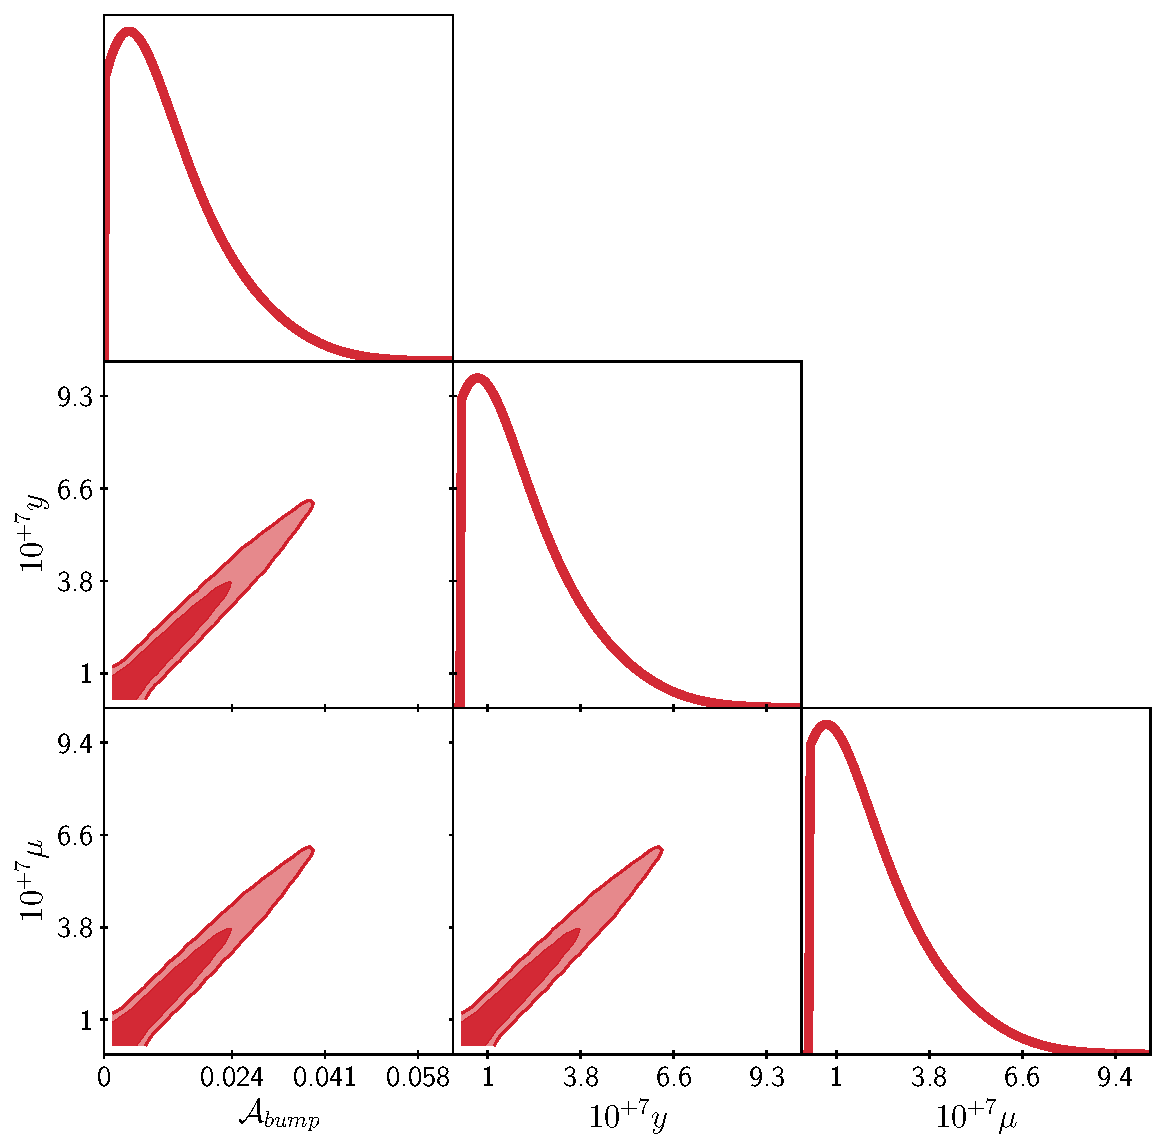
\includegraphics[width=0.7\textwidth]{Constraints/Lognormal.pdf}
        \caption{With nuisance}
        \label{fig:LN}        
    \end{subfigure}
    \hfill
    \begin{subfigure}{0.49\textwidth}
        \centering
        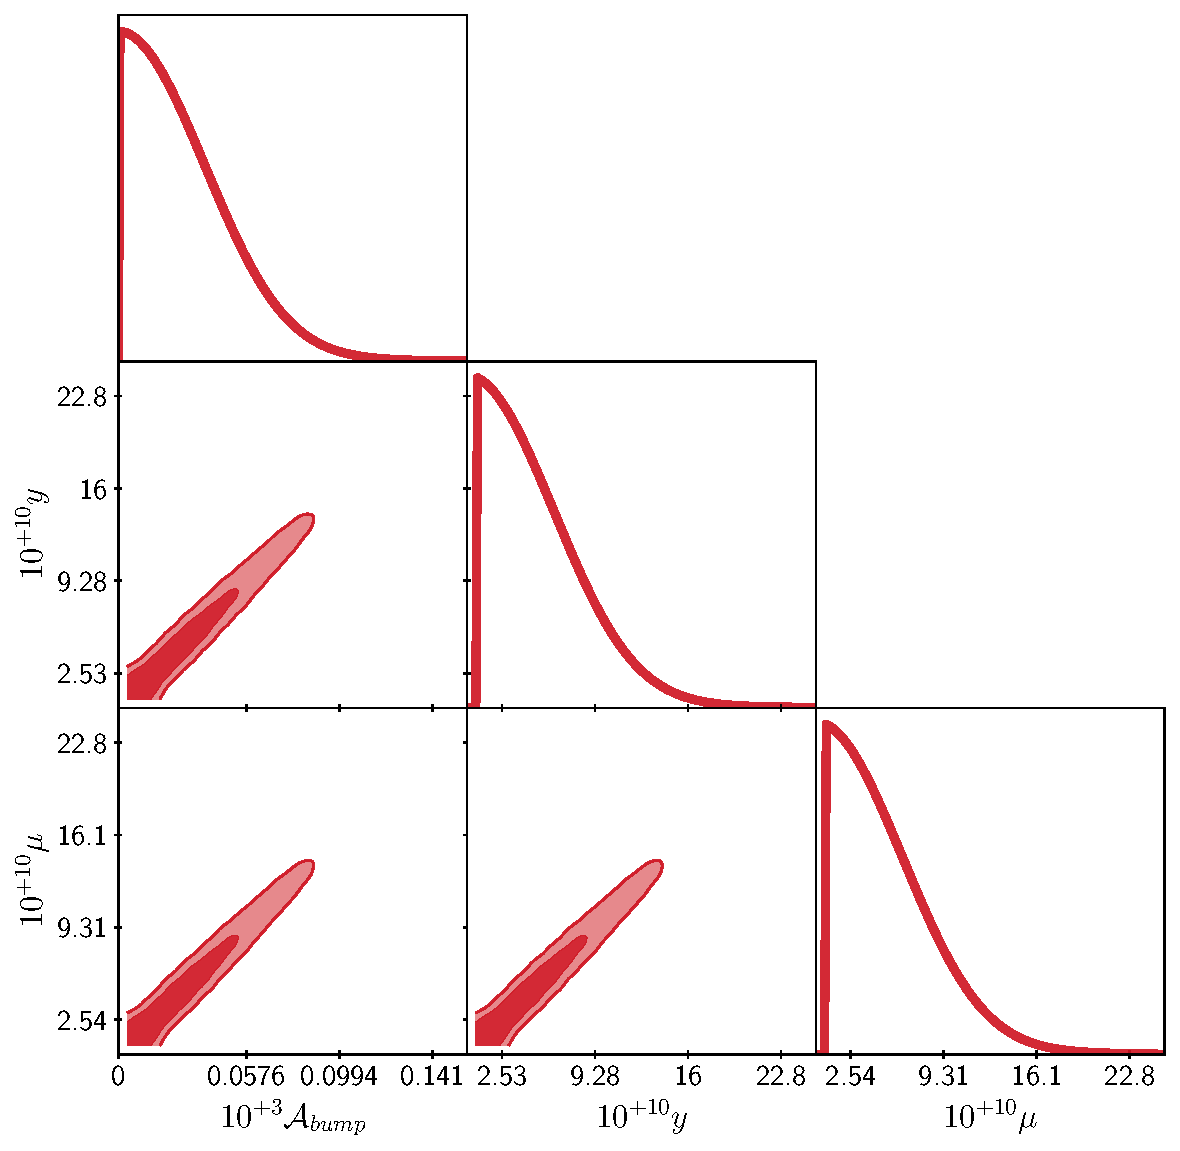
\includegraphics[width=0.7\textwidth]{Constraints/LN_NN.pdf}
        \caption{Without nuisance}
        \label{fig:LN_NN}        
    \end{subfigure}

    \vspace{1em}

    \begin{subfigure}{0.5\textwidth}
        \centering
        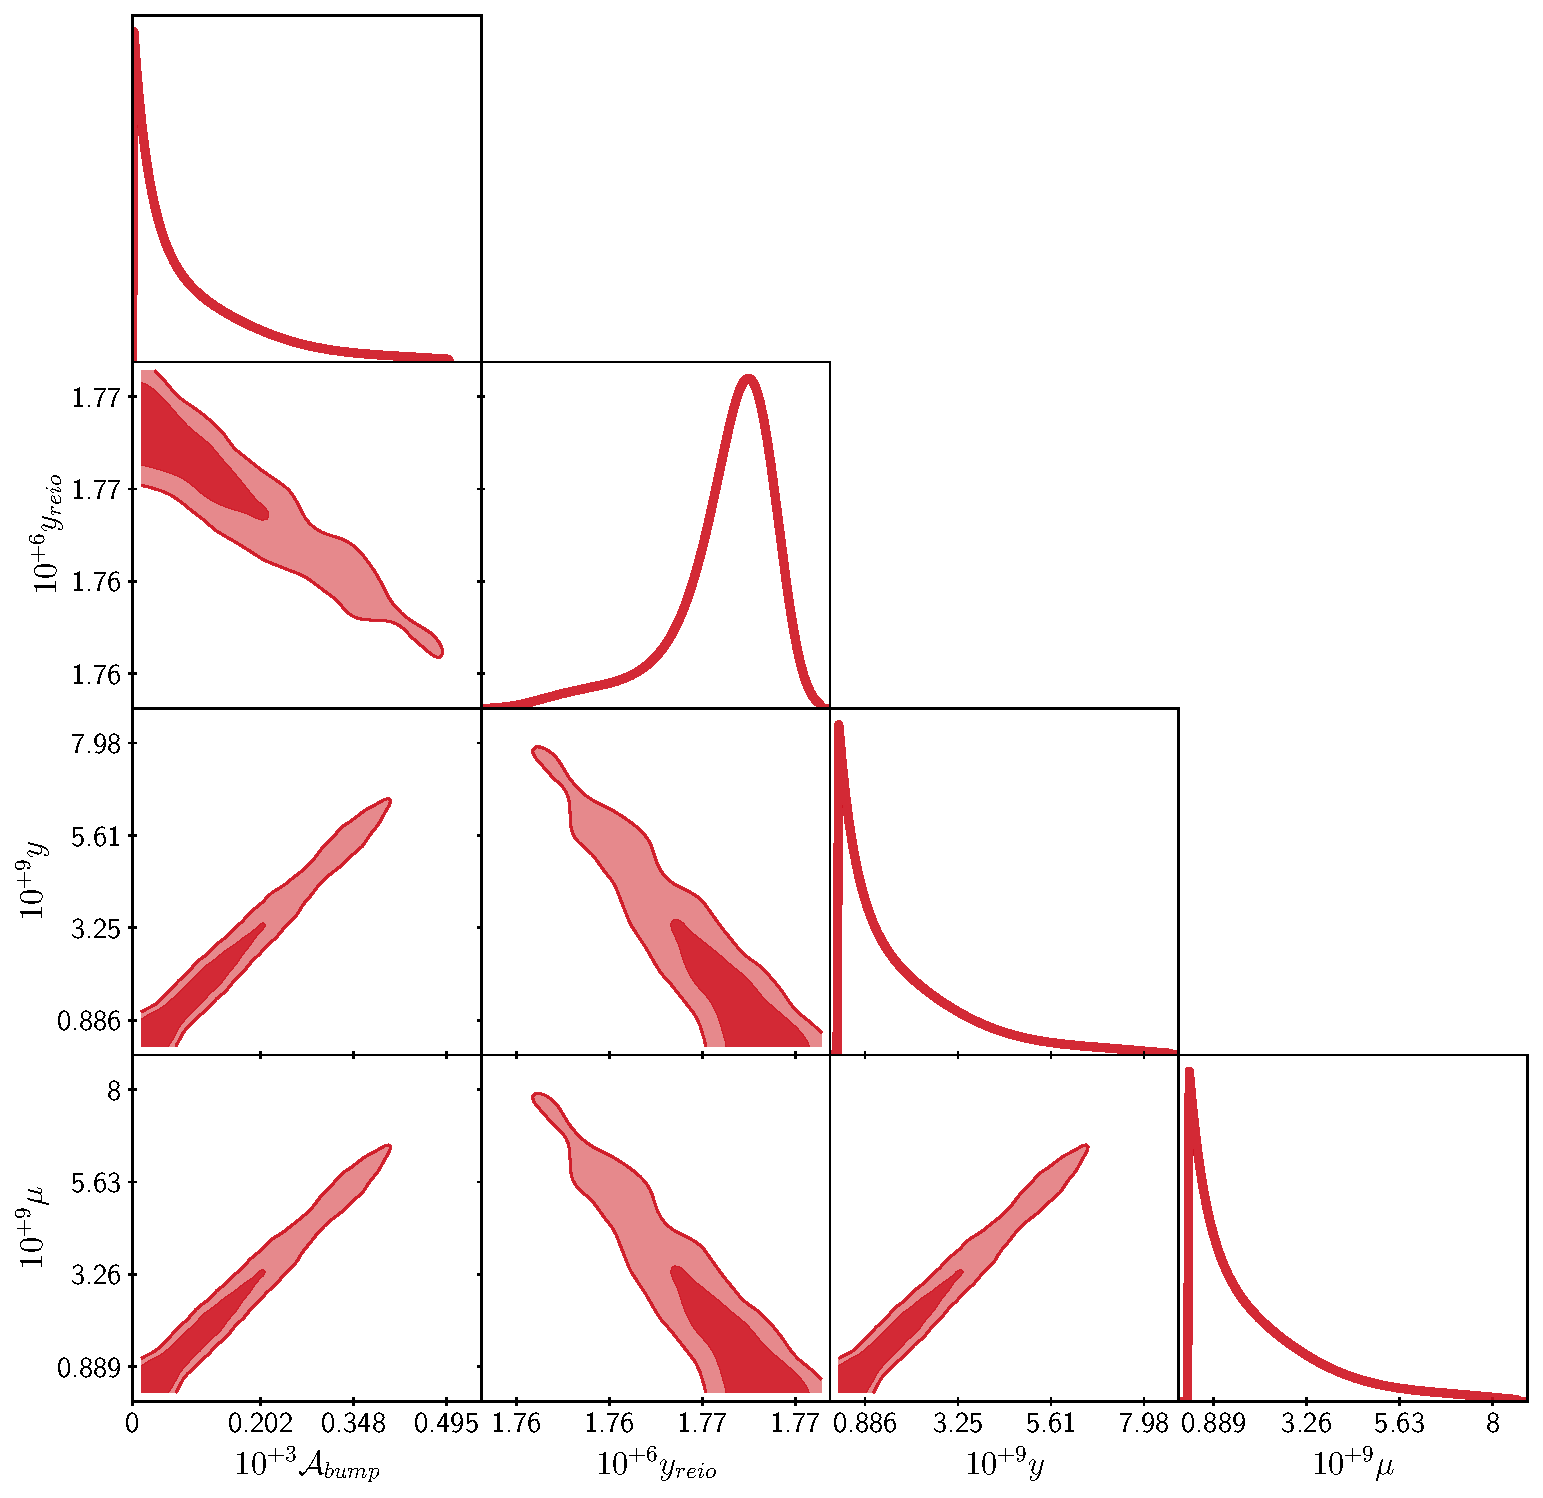
\includegraphics[width=0.7\textwidth]{Constraints/LN_NN_reio.pdf}
        \caption{Only $y_\text{reio}$ nuisance}
        \label{fig:LN_NN_reio}        
    \end{subfigure}
    \caption{Marginalized posterior distributions for the amplitude of a lognormal bump placed at $k_\text{pk}=10$ Mpc$^{-1}$ with width $\sigma_\text{bump}=0.44$. The three panels show the results obtained with different assumptions on the nuisance parameters.}
    \label{fig:LN_all}
\end{figure}




\appendix
\chapter{Differential geometry tools}
\section{Maximally symmetric spaces}\label{app:MaxSymm}
Consider $\mathbb{R}^n$, this space is highly symmetric: it is isotropic and homogeneous, or, in a simpler way, every point and every direction "look" the same.\\
This means that $\mathbb{R}^n$ is symmetric under every rotation and translation: in $n$-dimensions there are $n$ possible translations (along the $n$ axes) and $n\frac{n-1}{2}$ possible rotations (for each axis we can rotate it towards $n-1$ other axes and to avoid double counting $x\rightarrow y$ and $y\rightarrow x$ we divide by $2$), for a total number of symmetries equals to $$n+n\frac{n-1}{2}=n\frac{n+1}{2}.$$ 
An $n$-dimensional manifold is said to be \textbf{maximally symmetric} if it possesses the same number of symmetries of $\mathbb{R}^n$. In the differential geometry language, a symmetry is defined through isometries, that are diffeomorphisms under which the metric tensor is invariant.\\
For each symmetry of the metric we can define a \textbf{Killing vector}, which satisfies the Killing equation 
\begin{equation}
    0=(\pounds_{\vec K}g)_{\mu\nu}=\nabla_\mu K_\nu+\nabla_\nu K_\mu, \label{KillingEq}
\end{equation}
where $\pounds_{\vec{K}}$ is the Lie derivative along $\vec K$, which is the Killing vector.

We now want to show that a maximally symmetric space really possesses the maximum number of symmetries, namely the maximum number of independent\footnote{Linearly independent here means that $\not\exists$ a set of constants $c_n$ such that $$\sum_n c_n K_\mu^{(n)}(P)=0 \qquad \forall P\in\mathcal{M}.$$} Killing vectors.
Consider the defining equation of the Riemann tensor applied to a 1-form
\begin{equation}
    R^{\mu}_{\nu\rho\sigma}K_\mu=-[\nabla_\rho,\nabla_\sigma]K_\nu,\label{RiemannDef}
\end{equation}
this definition, combined with the algebraic Bianchi identity, ($R^\mu_{\nu\rho\sigma}+R^\mu_{\rho\sigma\nu}+R^\mu_{\sigma\nu\rho}=0 $) implies that each Killing vector must satisfy
$$\nabla_\rho\nabla_\sigma K_\nu-\nabla_\sigma\nabla_\rho K_\nu +\nabla_\sigma\nabla_\nu K_\rho-\nabla_\nu\nabla_\sigma K_\rho+\nabla_\nu\nabla_\rho K_\sigma-\nabla_\rho\nabla_\nu K_\sigma=0.$$
This equation can be simplified by the Killing equation \eqref{KillingEq}: using this relation we can sum pairs of terms obtaining $$ 2(\nabla_\rho\nabla_\sigma K_\nu-\nabla_\sigma\nabla_\rho K_\nu -\nabla_\nu\nabla_\sigma K_\rho)=0,$$ that using \eqref{RiemannDef} turns out to be the following
\begin{equation}
    R^\mu_{\nu\rho\sigma}K_\mu=\nabla_\nu\nabla_\sigma K_\rho. \label{RNabla}
\end{equation}
This equation shows that the second covariant derivative acts on Killing vectors just as a linear application. In this way we can determine every derivative of a Killing vector in a specific point, just by knowing its value and the value of its first covariant derivative, at the same point.\\
If we now Taylor expand the Killing vector around a point $P$, we will obtain some kind of expansion that depends on the value in $P$ of all covariant derivatives of all orders, however we showed that we can evaluate those just knowing $K_\mu(P)$ and $\nabla_\nu K_\mu(P)$. This means that we can express the Killing vector field as a combination of two functions that do not depend on the Killing vector itself or on its derivatives:
\begin{equation*}
    K_\mu(x)=A_\mu\phantom{}^\lambda(x,P)K_\lambda(P)+B_\mu\phantom{}^{\lambda\nu}(x,P)\nabla_\nu K_\lambda(P),
\end{equation*}
these functions depend only on $x$, the point $P$, and the metric, through the Riemann tensor. For this reason these must be the same functions for all Killing vectors:
\begin{equation}\label{KillingExp}
    K_\mu^{(n)}(x)=A_\mu\phantom{}^\lambda(x,P)K_\lambda^{(n)}(P)+B_\mu\phantom{}^{\lambda\nu}(x,P)\nabla_\nu K_\lambda^{(n)}(P).
\end{equation}
The above equation tells us that a given Killing vector is determined by $K_\lambda^{(n)}(P)$, which has $N$ possible independent values, and by $\nabla_\nu K_\lambda^{(n)}(P)$, which has $N\frac{N-1}{2}$ independent values, due to its antisymmetry (which is a consequence of the Killing equation \eqref{KillingEq}).\\
In this way we have shown that the maximum number of independent Killing vectors in an $N$-dimensional manifold is exactly the same number that possesses $\mathbb{R}^N$ $$N+N\frac{N-1}{2}=N\frac{N+1}{2}.$$

We want to conclude deriving the form that has the Riemann tensor in a maximally symmetric space.\\
In general, equation \eqref{RNabla} must hold for every Killing vector, furthermore it also must be consistent with the commutator of covariant derivatives \eqref{RiemannDef}. This requirement and the fact that we have the maximum number of linearly independent Killing vectors will determine the form of $R^\mu_{\nu\rho\sigma}$. Consider \eqref{RiemannDef} applied to the two indices tensor $$ [\nabla_\sigma,\nabla_\nu]\nabla_\mu K_\rho=-R^\lambda_{\mu\sigma\nu}\nabla_\lambda K_\rho-R^\lambda _{\rho\sigma\nu}\nabla_\mu K_\lambda,$$ the equation \eqref{RNabla} can be used to obtain 
\begin{align*}
    \nabla&_\sigma(R^\lambda_{\nu\rho\mu}K_\lambda)-\nabla_\nu(R^\lambda_{\sigma\rho\mu}K_\lambda)=\\&=\nabla_\sigma R^\lambda_{\nu\rho\mu}K_\lambda-\nabla_\nu R^\lambda_{\sigma\rho\mu}K_\lambda+\ R^\lambda_{\nu\rho\mu}\nabla_\sigma K_\lambda- R^\lambda_{\sigma\rho\mu}\nabla_\nu K_\lambda=-R^\lambda_{\mu\sigma\nu}\nabla_\lambda K_\rho-R^\lambda _{\rho\sigma\nu}\nabla_\mu K_\lambda.
\end{align*}
Now, Killing equation \eqref{KillingEq} allows us to move the index $\lambda$ to the covariant derivative in each term, then, using a bunch of Kronecker deltas we get $$ (\nabla_\sigma R^\lambda_{\nu\rho\mu}-\nabla_\nu R^\lambda_{\sigma\rho\mu})K_\lambda=(R^\lambda_{\nu\rho\mu}\delta_{\sigma}\phantom{}^\alpha-R^\lambda_{\sigma\rho\mu}\delta_{\nu}\phantom{}^\alpha+R^\lambda_{\mu\sigma\nu}\delta_{\rho}\phantom{}^\alpha-R^\lambda_{\rho\sigma\nu}\delta_{\mu}\phantom{}^\alpha)\nabla_\lambda K_\alpha.$$
This relation must hold for every Killing vector. We have the maximum number of independent Killing vectors, thus we can generate any other Killing vector from a combination of these. The general expansion \eqref{KillingExp} shows that a Killing vector field that vanishes in $P$, while its derivatives does not, can exists, and we surely can obtain it from a linear combination of the others. The above equation holds also for this one in $P$ only if the right-hand side vanishes too, this can happen only if the term in parentheses is symmetric in $\lambda\ \alpha$ (so that it vanishes when contracted with $\nabla_\lambda K_\alpha$ that is antisymmetric)$$R^\lambda_{\nu\rho\mu}\delta_{\sigma}\phantom{}^\alpha-R^\lambda_{\sigma\rho\mu}\delta_{\nu}\phantom{}^\alpha+R^\lambda_{\mu\sigma\nu}\delta_{\rho}\phantom{}^\alpha-R^\lambda_{\rho\sigma\nu}\delta_{\mu}\phantom{}^\alpha=R^\alpha_{\nu\rho\mu}\delta_{\sigma}\phantom{}^\lambda-R^\alpha_{\sigma\rho\mu}\delta_{\nu}\phantom{}^\lambda+R^\alpha_{\mu\sigma\nu}\delta_{\rho}\phantom{}^\lambda-R^\alpha_{\rho\sigma\nu}\delta_{\mu}\phantom{}^\lambda.$$
Contracting $\mu$ and $\alpha$, recalling that $R^\mu_{\nu\mu\rho }=R_{\nu\rho}$ and $R^\mu_{\mu\nu\rho}=0$, we find
$$R^\lambda_{\nu\rho\sigma}-R^\lambda_{\sigma\rho\nu}+R^\lambda_{\rho\sigma\nu}-NR^\lambda_{\rho\sigma\nu}=-R_{\nu\rho}\delta_\sigma\phantom{}^\lambda+R_{\sigma\rho}\delta_\nu\phantom{}^\lambda-R^\lambda_{\rho\sigma\nu},$$
here we recognize that, from the algebraic Bianchi identity, $$R^\lambda_{\sigma\rho\nu}=-R^\lambda_{\sigma\nu\rho}=R^\lambda_{\nu\rho\sigma}+R^\lambda_{\rho\sigma\nu},$$ which cancels two terms in the previous equation, that now reads, after having lowered one index, 
\begin{equation}\label{RN1}
    (N-1)R_{\lambda\rho\sigma\nu}=R_{\nu\rho}g_{\sigma\lambda}-R_{\sigma\rho}g_{\nu\lambda}.
\end{equation}
Notice that the above equation must be antisymmetric in $\lambda\ \rho$ (due to the proprieties of the Riemann tensor),$$
R_{\nu\rho}g_{\sigma\lambda}-R_{\sigma\rho}g_{\nu\lambda}=-R_{\nu\lambda}g_{\sigma\rho}+R_{\sigma\lambda}g_{\nu\rho},
$$ contracting $\lambda\ \nu$, this relation becomes 
\begin{equation}
    R_{\sigma\rho}-NR_{\sigma\rho}=-Rg_{\sigma\rho}+R_{\sigma\rho},\quad \Rightarrow\quad \boxed{R_{\sigma\rho}=\frac{R}{N}g_{\sigma\rho}},
\end{equation}
inserting this one into the \eqref{RN1} we get our final result
\begin{equation}
        \boxed{R_{\lambda\rho\sigma\nu}=\frac{R}{N(N-1)}(g_{\nu\rho}g_{\lambda\sigma}-g_{\sigma\rho}g_{\lambda\nu})}.
\end{equation}
\chapter{Thermodynamics tools}
\section{Small chemical potential approximation}
\label{sec:SmallChemicalPotential}
In this appendix we will show how to approximate the energy and number densities for a gas of photons in the presence of a small chemical potential.
The goal is to obtain corrections to  
$$\rho=a_RT^4,\qquad n=b_RT^3,$$ that are obtained from the Planck distribution.

Let's start from the number density, analogous calculations will then give the result for the energy density. From the definition we have
\begin{align}
    n&=\frac{g_\text{dof}}{(2\pi)^3}\int d^3p\ \frac{1}{\exp(\frac{\nu}{k_BT}+\mu)-1}=\frac{g_\text{dof}}{2\pi^2}\int_0^\infty dp \frac{p^2 }{\exp(\frac{\nu}{k_BT}+\mu)-1}\nonumber\\&\ \bigg\downarrow\qquad p=\nu,\qquad x\defeq\frac{\nu}{k_BT}\nonumber\\
    &=\frac{g_\text{dof}}{2\pi^2}(k_BT)^3\int_0^\infty dx \frac{x^2}{\exp(x+\mu)-1}=\frac{g_\text{dof}}{2\pi^2}(k_BT)^3\int_0^\infty dx \frac{x^2e^{-(x+\mu)}}{1-e^{-(x+\mu)}}\nonumber\\&=\frac{g_\text{dof}}{2\pi^2}(k_BT)^3\int_0^\infty dx\ x^2e^{-(x+\mu)}\sum_{n=0}^{\infty}e^{-n(x+\mu)}=\frac{g_\text{dof}}{2\pi^2}(k_BT)^3\sum_{n=0}^{\infty}\int_0^\infty dx\ x^2e^{-(n+1)(x+\mu)}\nonumber\\&=\frac{g_\text{dof}}{2\pi^2}(k_BT)^3\sum_{n=0}^{\infty}\frac{2}{(n+1)^3}e^{-(n+1)\mu}\approx\frac{g_\text{dof}}{2\pi^2}(k_BT)^3\sum_{n=0}^{\infty}2\frac{1-(n+1)\mu}{(n+1)^3}\nonumber\\&\ \bigg \downarrow\qquad \zeta(z)\defeq\sum_{n=1}^\infty\bigg(\frac{1}{n}\bigg)^z\qquad\text{Riemann zeta function}\nonumber\\
    &=\frac{g_\text{dof}}{\pi^2}(k_BT)^3\big[\zeta(3)-\mu\zeta(2)\big]=b_RT^3\bigg[1-\mu\frac{\zeta(2)}{\zeta(3)}\bigg]\,\label{eq:SmallChemicalPotential_n}
\end{align}
where in the last line we defined $b_R\defeq\frac{g_\text{dof}}{\pi^2}k_B^3\zeta(3)$ with $g_\text{dof}=2$.

The same calculation can be applied to the energy density, we just need to pay attention to the extra $\nu$ factor in the integrand: ultimately this will lead to a different integral inside the series expansion, hence different points of the zeta function will appear. Again from the definition and preceding as before
\begin{align}
    \rho&=\frac{g_\text{dof}}{(2\pi)^3}\int d^3p\ \frac{E}{\exp(\frac{\nu}{k_BT}+\mu)-1}=\frac{g_\text{dof}}{2\pi^2}\int_0^\infty dp \frac{p^3}{\exp(\frac{\nu}{k_BT}+\mu)-1}\nonumber\\
    &=\frac{g_\text{dof}}{2\pi^2}(k_BT)^4\sum_{n=0}^{\infty}\int_0^\infty dx\ x^3e^{-(n+1)(x+\mu)}\nonumber=\frac{g_\text{dof}}{2\pi^2}(k_BT)^4\sum_{n=0}^{\infty}\frac{6}{(n+1)^4}e^{-(n+1)\mu}\\&\approx\frac{g_\text{dof}}{2\pi^2}(k_BT)^4\sum_{n=0}^{\infty}6\frac{1-(n+1)\mu}{(n+1)^4}=\frac{3g_\text{dof}}{\pi^2}(k_BT)^4\big[\zeta(4)-\mu\zeta(3)\big]=a_RT^4\bigg[1-\mu\frac{\zeta(3)}{\zeta(4)}\bigg]\,\label{eq:SmallChemicalPotential_rho}
\end{align}
where we defined $a_R\defeq\frac{3g_\text{dof}}{\pi^2}k_B^4\zeta(4)=\frac{\pi^2}{15}k_B^4$ with $g_\text{dof}=2$.\\
\section{Scalar perturbed Liouville operator}\label{app:scalarPerturbedLiouvilleOperator}
In this appendix we will show how to obtain the perturbed Liouville operator, at first order, for the photon phase space in the presence of scalar perturbations. Since we are interested only in first order perturbations, in the next calculations, we will always neglect higher order contributions by Taylor expanding every function of the perturbations. We will work with the perturbed metric in the conformal Newtonian gauge, which is given by
$$ds^2=a^2(\eta)\left[-(1+2\Psi)d\tau^2+(1-2\Phi)\delta_{ij}dx^idx^j\right].$$
The Liouville operator, defined in , reads
$$\hat{\mathbf{L}}[f]=\frac{df}{d\tau}=\frac{\partial f}{\partial \tau}+\frac{\partial f}{\partial x^i}\frac{d x^i}{d\tau}+\frac{\partial f}{\partial p}\frac{d p}{d\tau}+\frac{\partial f}{\partial \hat p^i}\frac{d \hat p^i}{d\tau},$$
where $p^i=p\ \hat p^i$ (with $\hat p^i\hat p^j\delta_{ij}=1$) is the local 3-momentum of the photon, and we already considered that the local energy and the 3-momentum are not independent due to the mass-shell condition. We also assume that $f$ can also be expanded on a background, which corresponds to the black body radiation, plus a first order perturbation (see section \ref{sec:ThetaTimeEvolution} for more on this expansion). Note that, since the blackbody radiation is isotropic and homogeneous (it does not depend on $x^i$ or $\hat p^i$) the two factors $\frac{\partial f}{\partial x^i}$ and $\frac{\partial f}{\partial \hat p^i}$ are only first order contributions. This observation will simplify our calculations later on since it implies that $\frac{dx^i}{d\tau}$ and $\frac{d\hat p^i}{d\tau}$ are needed only at order zero.

Let's spend some time discussing local energy and momentum. The local energy is defined as the energy of a photon in the local rest frame of an observer, thus for a static observer ($U^\mu=(\frac{1-\Psi}{a},0,0,0)$) it reads
$$E=-U_\mu P^\mu=a(1+2\Psi)P^0(1-\Psi)\approx aP^0(1+\Psi).$$
The local momentum defined in the same way, therefore it must satisfy the usual Minkowskian mass-shell relation $E=\sqrt{p^ip^j\delta_{ij}}$. Using the mass-shell condition for the 4-momentum of the photon $P^\mu P_\mu=0$, we can write
\begin{align*}
    &P^\mu P_\mu=-a^2(1+2\Psi)(P^0)^2+a^2(1+2\Phi)P^iP^j\delta_{ij}=0,\\
    &\Rightarrow\quad P^0=\sqrt{\frac{1+2\Phi}{1+2\Psi}P^iP^j\delta_{ij}}\approx(1+\Phi-\Psi)\sqrt{P^iP^j\delta_{ij}},\\
    &E=\sqrt{p^ip^j\delta_{ij}}=aP^0(1+\Psi)=a(1+\Phi)\sqrt{P^iP^j\delta_{ij}}.
\end{align*}
In this way we identify $p^i=a(1+\Phi)P^i$ as the local 3-momentum. Note that it follows from $E=\sqrt{p^ip^j\delta_{ij}}$ that decomposing $p^i=p\ \hat p^i$ then $p=E$, as we expect in the local reference frame.

We are now ready to determine all the contribution to the Liouville operator. First, from the above discussion on the local energy and momentum, we recognize that 
\begin{equation}\label{eq:B.1}
    \frac{dx^i}{d\tau}=\frac{P^i}{P^0}=\frac{(1-\Phi)p^i}{(1+\Psi)E}\approx \hat p^i(1-\Psi-\Phi).
\end{equation}
Then we have to evaluate $$\frac{dp}{d\tau}=\frac{d}{d\tau}aP^0(1+\Psi)=\mathcal{H}p+a(1+\Psi)\frac{dP^0}{d\tau}+p\Psi',$$
therefore we need to compute $\frac{dP^0}{d\tau}$. This can be accomplished by using the geodesic equation $$ \frac{dP^0}{d\tau}=\frac{dP^0}{d\lambda}\frac{1}{P^0}=-\frac{\Gamma^0_{\mu\nu}}{P^0}P^\mu P^\nu,$$
in the conformal Newtonian gauge the relevant Christoffel symbols are $$\Gamma^0_{00}=\mathcal{H}+\Psi',\quad\Gamma^0_{0i}=\Psi,_i,\quad\Gamma^0_{ij}=\bigg[\mathcal{H}(1+2\Phi-2\Psi)+\Phi' \bigg]\delta_{ij}.$$
In this way we get
\begin{align}\label{eq:B.2}
    \frac{dp}{d\tau}&=(\mathcal{H}+\Psi') p-a(1+\Psi)\times\nonumber\\&\qquad\qquad\qquad\times \bigg[(\mathcal{H} +\Psi')P^0+P^i\Psi,_i+\big(\mathcal{H}(1+2\Phi-2\Psi)+\Phi' \big)\frac{P^iP^j\delta_{ij}}{P^0} \bigg]\nonumber\\
    &\approx\mathcal{H} p-\mathcal{H} p+\Psi'p-\Psi'p-p^i\Psi,_i-\mathcal{H}p-\Phi'p\nonumber\\
    &=-\mathcal{H} p-\Phi' p-p^i\Psi,_i
\end{align}
We now have to obtain
$$\frac{d\hat p^i}{d\tau}=\frac{d}{d\tau}\frac{p^i}{p}=\frac{dp^i}{d\tau}\frac{1}{p}-\frac{dp}{d\tau}\frac{p^i}{p^2},$$
in which we can get $\frac{dp^i}{d\tau}$ by \eqref{eq:B.2} noting
$$\frac{dp}{d\tau}=\frac{d}{d\tau}\sqrt{p^ip^j\delta_{ij}}=\frac{p^j}{p}\frac{dp^i}{d\tau}\delta_{ij}.$$
These two simple calculations, with equation \eqref{eq:B.2}, show that $\frac{d\hat p^i}{d\tau}$ has no zeroth order contributions, but only first order ones. Therefore, when multiplied by $\frac{\partial f}{\partial \hat p^i}$ a second order, in perturbations, term is generated, and for this reason we will neglect its contributions.

Inserting equations \eqref{eq:B.1} and \eqref{eq:B.2} into the Liouville operator we end up with
\begin{align}\label{eq:Liouville_scalar_perturbed}
    \hat{\mathbf{L}}[f]&=\frac{\partial f}{\partial \tau}+\hat p^i\frac{\partial f}{\partial x^i}-p\bigg(\mathcal{H}-\frac{\partial \Phi}{\partial \tau}+\frac{\partial \Phi}{\partial x^i}\hat p^i\bigg)\frac{\partial f}{\partial p},\nonumber\\
    &\bigg\downarrow\quad\text{moving to cosmic time } dt=a\ d\tau,\nonumber\\
    \hat{\mathbf{L}}[f]&=\frac{\partial f}{\partial t}+\frac{\hat p^i}{a}\frac{\partial f}{\partial x^i}-p\bigg(H-\frac{\partial \Phi}{\partial t}+\frac{\partial \Phi}{\partial x^i}\frac{\hat p^i}{a}\bigg)\frac{\partial f}{\partial p}
\end{align}
\section{Tensor perturbed Liouville operator}\label{app:tensorPerturbedLiouvilleOperator}
Previously, we considered how scalar perturbations of the metric (which are in general the most studied) contributes to the evolution of the phase space associated to photons. Now, we are going to follow the same steps to study instead the effects of tensor perturbations. Again keep in mind that we will only consider first order perturbations and higher contributions will be neglected.

Tensor perturbations are described by the transverse traceless tensor $h_{ij}$, which happens to be gauge invariant (section ). At first order in perturbation theory the tensor perturbed metric thus reads 
$$ds^2=a^2(-d\tau^2+(\delta_{ij}+h_{ij})dx^idx^j).$$
The Liouville operator, as usual, is defined as
$$\hat{\mathbf{L}}[f]=\frac{df}{d\tau}=\frac{\partial f}{\partial \tau}+\frac{\partial f}{\partial x^i}\frac{d x^i}{d\tau}+\frac{\partial f}{\partial p}\frac{d p}{d\tau}+\frac{\partial f}{\partial \hat p^i}\frac{d \hat p^i}{d\tau},$$
where $p^i=p\ p^i$ is again the local 3-momentum, note that even though its definition (as the momentum observed by a static observer) won't change, its relation to the 4-momentum is changed due to the different metric considered. Now, indeed the local energy is
$$U^\mu=(a^{-1},0,0,0)\ \Rightarrow\ E=-U_\mu P^\mu= aP^0$$
and then requiring that $E=\sqrt{p^ip^j\delta_{ij}}=p$ we observe that the form of the local 3-momentum should be
\begin{align*}
    P^\mu P_\mu&=-a^2\big(P^0\big)^2+a^2(\delta_{ij}+h_{ij})P^iP^j=0\quad\Rightarrow \quad\big(P^0\big)^2=(\delta_{ij}+h_{ij})P^iP^j\\E^2&=p_ip_j\delta_{ij}=\big(aP^0\big)^2=a^2(\delta_{ij}+h_{ij})P^iP^j\quad\Rightarrow \quad p_i=a(\delta_{ij}+\frac{1}{2}h_{ij})P^j,
\end{align*} 
where we used that there is no difference between covariant e contravariant vectors for the local momentum since in the local reference frame the spatial metric is the identity.

We can now proceed and evaluate the first contribution to the Liouville operator $\frac{dx^i}{d\tau}$, keeping in mind that (as in appendix \ref{app:scalarPerturbedLiouvilleOperator}) we only need order zero contributions.
\begin{equation}\label{eq:B.4}
    \frac{dx^i}{d\tau}=\frac{P^i}{P^0}=\frac{p_j}{E}\bigg(\delta^{ij}-\frac{1}{2}h^{ij}\bigg)\approx\frac{p^i}{E}.
\end{equation}
The second factor is instead needed up to the first order. We start by evaluating
$$\frac{dp}{d\tau}=\frac{d}{d\tau}aP^0=\mathcal{H} p+a\frac{dP^0}{d\tau}=\mathcal{H} p-\frac{a}{P^0}\Gamma^0_{\mu\nu}P^\mu P^\nu,$$
where in the last step we used the geodesic equation. With the metric in consideration the relevant Christoffel symbols read:
$$\Gamma^0_{00}=\mathcal{H},\qquad \Gamma^0_{0i}=0,\qquad\Gamma^{0}_{ij}=\mathcal{H} (\delta_{ij}+h_{ij})+\frac{1}{2}h'_{ij}.$$
With these, recalling that $p^2=a^2(\delta_{ij}+h_{ij})P^i P^j$ and that at order zero $p^\mu=aP^\mu$, we finally get
\begin{equation}\label{eq:B.5}
   \frac{dp}{d\tau}=-\frac{a}{P^0}\bigg[\mathcal{H} (\delta_{ij}+h_{ij})-\frac{1}{2}h'_{ij}\bigg]P^i P^j=-\mathcal{H}p-\frac{1}{2}h'_{ij}\hat p^i\hat p^j.
\end{equation}
We are left with $\frac{d\hat p^i}{d\tau}$ to be evaluated, however as in appendix \ref{app:scalarPerturbedLiouvilleOperator}, we can show that this gives no zeroth order contribution, generating in the Liouville operator a second order term (since $\frac{\partial f}{\partial\hat p^i}$ has to be of first order too since the unperturbed distribution is isotropic) that can be neglected.

Summing all up we get that the Liouville operator now reads
\begin{align}\label{eq:tensorPerturbedLiouvilleOperator}
   \hat{\mathbf{L}}[f]&=\frac{\partial f}{\partial\tau}+\hat p^i\frac{\partial f}{\partial x^i}-\frac{1}{2}\frac{\partial f}{\partial \tau}h'_{ij}\hat p^i\hat p^j\nonumber&&\\
   &\bigg\downarrow\quad\text{moving to cosmic time } dt=a\ d\tau,\nonumber&&\\
   \hat{\mathbf{L}}[f]&=\frac{\partial f}{\partial t}+\frac{\hat p^i}{a}\frac{\partial f}{\partial x^i}-\frac{1}{2}\frac{\partial f}{\partial t}\dot{h}_{ij}\hat p^i\hat p^j.&&
\end{align}
\chapter{Special functions}
\label{app:special-functions}
In this last appendix we recollect all the useful relations and definitions that we used with the many special functions we encountered. More detailed material to use special function can be found in the Abramowitz and Stegun \cite{abramowitz+stegun}.

\section{Spherical harmonics \(Y_{\ell m}(\theta,\varphi)\)}
\label{app:spherical-harmonics}
Spherical harmonics arise naturally when solving problems with spherical symmetry, such as phenomenon in the sky, since they are eigenfunction of the angular part of the Laplacian operator 
$$
\Bigg[\frac{1}{\sin\theta}\frac{\partial}{\partial \theta}\bigg(\sin\theta\frac{\partial}{\partial\theta}\bigg)+\frac{1}{\sin^2\theta}\frac{\partial^2}{\partial\phi^2}\Bigg]Y_{\ell,m}=-\ell(\ell+1)Y_{\ell,m},\qquad \frac{\partial}{\partial\phi}Y_{\ell,m}=im Y_{\ell,m},$$
where $\ell$ is a positive integer and $m$ is an integer with $|m|\leq \ell$.\\
Solving explicitly this equation yields for the first values of $\ell$ and $m$
\begin{align*}
&Y_{00}(\theta,\phi)=\frac{1}{\sqrt{4\pi}}, &Y_{1,0}(\theta,\phi)=i\sqrt\frac{3}{4\pi}\cos{\theta},\\ &Y_{1,\pm1}(\theta,\phi)=\mp i\sqrt\frac{3}{8\pi}\sin\theta e^{\pm i\phi},\quad
&Y_{20}(\theta,\phi)=\sqrt\frac{5}{16\pi}\big(1-3\cos^2\theta\big), \\ &Y_{2,\pm1}(\theta,\phi)=i\sqrt\frac{15}{8\pi}\cos{\theta}\sin\theta e^{\pm i\phi},\quad &Y_{2,\pm2}(\theta,\phi)=-\sqrt\frac{15}{32\pi}\sin^2\theta e^{\pm i2\phi},
\end{align*}
where all the coefficients have been determined by using the orthonormality relation
\[
\int\sin\theta\ d\theta d\phi\ Y_{\ell m}(\theta,\varphi)\,Y^*_{\ell' m'}(\theta,\varphi)
=\delta_{\ell\ell'}\delta_{mm'},
\]
which holds on the sphere since spherical harmonics represent an orthonormal basis of functions on such domain.\\
We conclude our discussion on spherical harmonics by giving the conjugation and parity relations  
\[
Y_{\ell m}^*(\theta,\varphi)=(-1)^m Y_{\ell,-m}(\theta,\varphi),\qquad
Y_{\ell m}(-\versor n)=(-1)^\ell Y_{\ell m}(\versor n),
\]
where the shorthand notation $\versor n$ has been used to indicate the angles associated to such direction.


\section{Legendre polynomials \(P_\ell(x)\)}
\label{app:legendre}
Legendre polynomials can be defined as the eigenfunctions of the Legendre equation 
\[
(1-\mu^2)P_\ell''(\mu)-2xP_\ell'(\mu)+\ell(\ell+1)P_\ell(\mu)=0,\qquad \mu\in[-1,1].
\]
The first three Legendre polynomials are 
$$
P_0(\mu)=1,\qquad P_1(\mu)=\mu,\qquad P_2(\mu)=\frac{3\mu^2-1}{2},
$$
while an explicit expression can be found for higher $\ell$ values by the \emph{Bonnet's formula}
\[
(\ell+1)P_{\ell+1}(\mu)=(2\ell+1)\mu P_\ell(\mu)-\ell P_{\ell-1}(\mu).
\]
We can observe that for $\ell=0,1,2$ (but this proprieties holds for all $\ell$) the polynomials are even or odd functions depending on whether $\ell$ is even or odd, respectively.\\
Note that the differential equation for spherical harmonics, assuming no $\phi$ dependence and defining $x\defeq\cos\theta$, turns into the Legendre equation above. This shows that we can match, up to the normalization factor, Legendre polynomials with $m=0$ spherical harmonics.
\[
Y_{\ell 0}(\theta,\varphi)=\sqrt{\frac{2\ell+1}{4\pi}}\,P_\ell(\cos\theta).
\]
Furthermore, a geometrical meaning can be attributed to the variable $\mu$, which now represents the scalar product between the versor $\versor n$ and the $z$-axis.\\
As for spherical harmonics, Legendre polynomials are an orthogonal basis on their domain $[-1,1]$
\[
\int_{-1}^{1}d\mu\ P_\ell(\mu)P_{m}(\mu)=\frac{2}{2\ell+1}\delta_{\ell m}.
\]
We conclude by giving a really useful formula that allows for Legendre polynomials to be turned in products of spherical harmonics and vice versa.
$$
P_\ell(\versor n\cdot\versor n')=\frac{4\pi}{2\ell+1}\sum_{m=-\ell}^\ell Y_{\ell,m}(\versor n)Y^*_{\ell,m'}(\versor n').$$



\section{Spin-weighted spherical harmonics \({}_sY_{\ell m}(\theta,\varphi)\)}
\label{app:spin-weighted}
A generalization of the spherical harmonics we have previously introduced are the \textbf{spin-weighted spherical harmonics}, which are used to expand the polarization anisotropies of the CMB. 
For our purpose it is not important to enter in the detail of this kind of functions, it is enough to keep in mind that they form na orthogonal set,
\[
\int_{S^2} Y^s_{\ell m}\,Y^{s*}_{\ell' m'}\,d\Omega=\delta_{\ell\ell'}\delta_{mm'},
\]
and the following conjugation proprieties holds
\[
\big(Y^s_{\ell m}(\theta,\varphi)\big)^*=(-1)^{m+s}Y^{-s}_{\ell,-m}(\theta,\varphi).
\]
A more detailed treatment of this kind of functions can be found in the work of Hu and White \cite{HuWhite}. 

\section{Bessel functions \(J_\nu(z), Y_\nu(z)\) and Hankel functions $H_\nu^{(1)}(z), H_\nu^{(2)}(z)$}
\label{app:bessel}
Bessel functions constitute the natural basis for problems with circular or cylindrical symmetry. They are solutions of the Bessel equation
\[
\frac{d^2J_\nu}{dz^2}+\frac{1}{z}\frac{dJ_\nu}{dz}+\bigg(1-\frac{\nu^2}{z^2}\bigg)J_\nu=0,
\]
where the parameter $\nu\in\mathbb C$ determines the specific solution. For non-integer values of $\nu$, $J_\nu$ and $J_{-\nu}$, which are both solutions of the above, are linearly independent, which means that their combination gives the full solution. However, for integer values of $\nu$ they become related by 
$$J_{-n}(z)=(-1)^n J_n(z), \qquad (n\in\mathbb Z) $$
and therefore a new linearly independent solution must be found. The \emph{Bessel function of the second kind}, also sometimes known as \emph{Neumann fucntion}, manages to remain linearly independent for all the values of $\nu$
$$Y_\nu(z)\defeq\frac{J_\nu(z)\cos(\nu\pi)-J_{-\nu}(z)}{\sin(\nu\pi)}.$$
On the other hand $J_\nu(z)$ is usually referred to as the \emph{Bessel function of the first kind}.\\
For small values of $z$ the last term of the Bessel equation dominates and the $z\to0$ limit is found to be
\[
J_\nu(z)\xrightarrow{z\to0}\frac{1}{\Gamma(\nu+1)}\left(\frac{z}{2}\right)^\nu,\qquad
Y_\nu(z)\xrightarrow{z\to0} -\frac{\Gamma(\nu)}{\pi}\left(\frac{2}{z}\right)^\nu,
\]
for which we can see that $J_\nu$ is regular for $z=0$ while $Y_\nu$ diverges. On the other hand, in the limit $z\to \infty$ the Bessel equation reduces to the equation of motion of a simple harmonic oscillator, and indeed the large $z$ asymptotic behavior results in 
\[
J_\nu(z)\xrightarrow{z\to\infty}\sqrt{\frac{2}{\pi z}}\cos\Big(z-\frac{\pi\nu}{2}-\frac{\pi}{4}\Big),\qquad
Y_\nu(z)\xrightarrow{z\to\infty}\sqrt{\frac{2}{\pi z}}\sin\Big(z-\frac{\pi\nu}{2}-\frac{\pi}{4}\Big).
\]
This can be better captured by defining the \emph{Hankel functions}, also known as \emph{Bessel functions of the third kind},
\[
H^{(1)}_\nu(z)=J_\nu(z)+iY_\nu(z),\qquad H^{(2)}_\nu(z)=J_\nu(x)-iY_\nu(z).
\]
From our discussion we immediately obtain the large $z$ limit
\[
H^{(1)}_\nu(z)\xrightarrow{x\to\infty}\sqrt{\frac{2}{\pi z}}\,e^{i\left(z-\frac{\pi\nu}{2}-\frac{\pi}{4}\right)},
\qquad
H^{(2)}_\nu(z)\xrightarrow{x\to\infty}\sqrt{\frac{2}{\pi z}}\,e^{-i\left(z-\frac{\pi\nu}{2}-\frac{\pi}{4}\right)}.
\]
Similarly, for small $z$ we have
\[
H^{(1)}_\nu(z)\xrightarrow{z\to0} -\frac{i}{\pi}\Gamma(\nu)\left(\frac{2}{z}\right)^\nu
\quad H^{(2)}_\nu(z)\xrightarrow{z\to0} \frac{i}{\pi}\Gamma(\nu)\left(\frac{2}{z}\right)^\nu.
\]

\section{Spherical Bessel functions \(j_\ell(z), y_\ell(z)\)}
\label{app:sph_bessel}
Spherical Bessel functions are the generalization of Bessel functions to problems in which spherical symmetry manifests. They are solutions of the following differential equation
$$\frac{d^2j_\ell}{dz^2}+\frac{2}{z}\frac{dj_\ell}{dz}+\bigg(1-\frac{\ell(\ell+1)}{z^2}\bigg)j_\ell=0,$$
and they can also be reconducted to the ordinary Bessel functions by
\[
j_\ell(z)=\sqrt{\frac{\pi}{2z}}\,J_{\ell+1/2}(z),\qquad
y_\ell(x)=\sqrt{\frac{\pi}{2z}}\,Y_{\ell+1/2}(z).
\]
From the above all the proprieties of the Bessel functions can be also applied to their spherical counterparts.\\
A really important relation that we used several times is the recursive relation which allows computing derivatives of these fucntions
$$j'_\ell(z)=j_{\ell-1}(z)-\frac{\ell+1}{z}j_\ell(z)=\frac\ell zj_\ell(z)-j_{\ell+1}(z),$$
which holds also for $y_\ell(z).$\\Finally, the following recursion relation holds
$$j_{\ell+1}(z)=\frac{2\ell+1}{z}j_\ell(z)-j_{\ell-1}(z),$$
which again holds also for $y_\ell(z)$.
 
\section{Gamma function \(\Gamma(z)\)}
\label{app:gamma}
The Euler gamma function is the generalization of the factorial operator over the right part ($\text{Re}(z)>0$) of the complex plane
\[
\Gamma(z)=\int_0^\infty t^{z-1}e^{-t}\,dt,\quad\Rightarrow\quad \Gamma(z+1)=z\Gamma(z).
\]
This implies that half integer arguments can be used in this generalized factorial: indeed by knowing $\Gamma(1/2)$ we can then infer by recursion all the next half integer values 
\[
\Gamma\!\left(1/2\right)=\sqrt{\pi},\qquad
\Gamma\!\left(3/2\right)=\frac{\sqrt{\pi}}{2},\qquad\dots
\]

\section{Riemann zeta function \(\zeta(s)\)}
\label{app:zeta}
Lastly, let's introduce the Riemann zeta function, which we used several times to simplify integrals.
This function is defined by the following integral  
\[
\zeta(z)\defeq\frac{1}{\Gamma(z)}\int dx\frac{x^{z-1}}{e^x-1},\qquad z\in \mathbb C.
\]
When the real part of $z$ is grater then 1, then one can show that the above integral can be written as a series
$$\zeta(z)=\sum_{n=1}^{\infty}\frac{1}{n^z}$$
We conclude by quoting some important values of the zeta function 
\[
\zeta(2)=\frac{\pi^2}{6},\qquad
\zeta(3)\approx 1.202056\ ,\qquad
\zeta(4)=\frac{\pi^4}{90}.
\]





\bibliographystyle{plain} 
\bibliography{references}  

\end{document}